\chapter{Linear Transformations and Matrices} \label{ch 2}

\begin{note}
In this chapter we consider those \emph{functions} defined \emph{on vector spaces} that in some sense ``preserve'' the structure.
These special functions are called \textbf{\LTRAN{}s}.
Some examples of \LTRAN{}:
Differentiation and integration in Calculus;
Rotations, reflections, and projections in geometry.
\end{note}

\begin{remark} \label{remark 2.0.1}
Throughout this chapter, we assume that all vector spaces are over a common field \(F\) unless explicitly stated.
\end{remark}

\section{Linear Transformations, Null Spaces, and Ranges} \label{sec 2.1}

\begin{definition} \label{def 2.1}
Let \(V\) and \(W\) be vector spaces over the same field \(F\).
We call a function \(\T: V \to W\) a \textbf{\LTRAN{} from \(V\) to \(W\)} if, for all \(x, y \in V\) and \(c \in F\), we have
\begin{enumerate}
\item \(\T(x + y) = \T(x) + \T(y)\) and
\item \(\T(cx) = c\T(x)\).
\end{enumerate}
We often simply call \(\T\) \textbf{linear}.
If \(V = W\), then we call \(\T\) a \textbf{linear operator} on \(V\).
\end{definition}

\begin{remark} \label{remark 2.1.1}
If the underlying field \(F\) is the field of \emph{rational} numbers, then \DEF{2.1} (a) implies (b) (see \EXEC{2.1.38}),
but, in general (a) and (b) are \emph{logically} independent.
See \EXEC{2.1.39} and \EXEC{2.1.40}.
\end{remark}

\begin{remark} \label{remark 2.1.2}
Now you can see why \RMK{2.0.1} assume all vector spaces have common field \(F\), because from \DEF{2.1}, we use the scalar \(c \in F\) on both the input vector \(v \in V\) to get scalar multiplication \(c v\), and the output vector \(\T(v) \in W\) to get scalar multiplication \(c \T(v)\).
So \(v, \T(v)\) are in \emph{different} vector space \(V\) and \(W\).
If \(W, V\) are also over different field, then one of these scalar multiplications will not even be well-defined.
\end{remark}

\begin{additional theorem} \label{athm 2.1}
Given any function \(\T : V \to W\) (where \(V, W\) are vector spaces over a command field \(F\)):
\begin{enumerate}
\item If \(\T\) is linear, then \(\T(\OV) = \OW\).
\item \(\T\) is linear if and only if \(\T(cx + y) = c\T(x) + \T(y)\) for all \(x, y \in V\) and \(c \in F\).
\item If \(\T\) is linear, then \(\T(x - y) = \T(x) - \T(y)\) for all \(x, y \in V\).
    (\(x - y\) (or \(\T(x) - \T(y)\)) is just a ``syntactic sugar'' for \(x + (-y)\)(or \(\T(x) + (-\T(y))\)).)
\item \(\T\) is linear if and only if, for \(x_1, x_2, ..., x_n \in V\) and \(a_1, a_2, ..., a_n \in F\), we have
\[
    \T \Big( \sum_{i = 1}^{n} a_i x_i \Big) = \sum_{i = 1}^{n} a_i \T(x_i).
\]
\end{enumerate}
And we generally use (b) to prove that a given function is linear.
\end{additional theorem}

\begin{proof} \ 
\begin{enumerate}
\item
Suppose \(\T\) is linear.
Then
\begin{align*}
    \T(\OV) & = \T(v + (-v)) & \text{for some \(v \in V\)} \\
           & = \T(v) + \T(-v) & \text{by \DEF{2.1}(a)} \\
           & = \T(v) + (-\T(v)) & \text{by \DEF{2.1}(b)} \\
           & = \OW. & \text{by (VS 4) of \(W\)}
\end{align*}

\item
\(\Longrightarrow\): Suppose \(\T\) is linear.
Then given \(x, y \in V\) and \(c \in F\),
\begin{align*}
    \T(cx + y) & = \T(cx) + \T(y) & \text{by \DEF{2.1}(a)} \\
              & = c\T(x) + \T(y) & \text{by \DEF{2.1}(b)}
\end{align*}

\(\Longleftarrow\):
Suppose given \(x, y \in V\) and \(c \in F\), \(\T(cx + y) = c\T(x) + \T(y)\).
Then in particular, let \(y = \OV\),
\begin{align*}
    \T(cx) & = \T(cx + \OV) & \text{by (VS 3) of \(V\)} \\
           & = \T(cx + y) \\
           & = c\T(x) + \T(y) & \text{by assumption} \\
           & = c\T(x) + \T(\OV) \\
           & = c\T(x) + \OW & \text{by part(a)} \\
           & = c\T(x) & \text{by (VS 3) of \(W\)}
\end{align*}
And in particular, let \(c = 1\),
\begin{align*}
    \T(x + y) & = \T(1x + y) & \text{by (VS 5) of \(V\)} \\
              & = \T(cx + y) \\
              & = c\T(x) + \T(y) & \text{by assumption} \\
              & = 1\T(x) + \T(y) \\
              & = \T(x) + \T(y) & \text{by (VS 5) of \(W\)}
\end{align*}
So by \DEF{2.1}, \(\T\) is linear.

\item
Suppose \(\T\) is linear, and \(x, y \in V\).
Then
\begin{align*}
    \T(x - y) & = \T(x + (-y)) & \text{unwrap ``syntactic sugar''} \\
             & = \T(x) + \T(-y) & \text{by \DEF{2.1}(a)} \\
             & = \T(x) + (-\T(y)) & \text{by \DEF{2.1}(b)} \\
             & = \T(x) - \T(y) & \text{add the syntactic sugar back}
\end{align*}

\item
This is immediately true with \DEF{2.1}(a)(b) and induction.
\end{enumerate}
\end{proof}

\begin{example} \label{example 2.1.1}
(Clearly) The function
\[
    \T : \SET{R}^2 \to \SET{R}^2 \text{ by } \T(a_1, a_2) = (2 a_1 + a_2, a_1)
\]
is linear.
\end{example}

\begin{remark} \label{remark 2.1.3}
In general, (informally but trivially,) given \(\T : F^n \to F^m\), if the each component of the output is a linear combination of the components of the input, then \(\T\) is linear.
\end{remark}

\begin{note}
As we will see in \CH{6}, the applications of linear algebra to geometry are wide and varied.
The main reason for this is that \emph{most of the important geometrical transformations are linear}.
Three particular transformations that we now consider are \textbf{rotation, reflection, and projection}.
We leave the proofs of linearity to the reader.
\end{note}

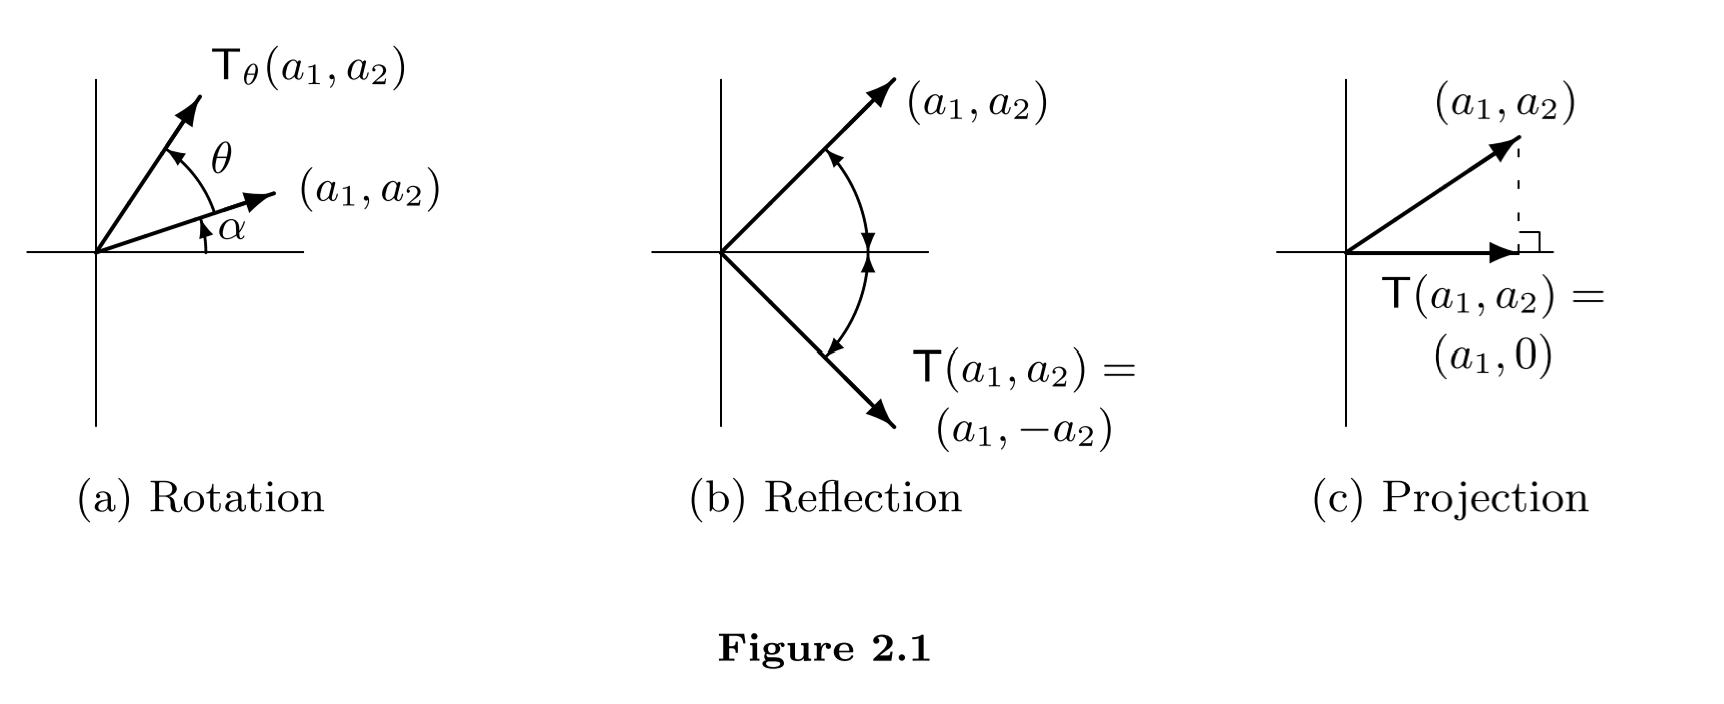
\includegraphics[width=16cm]{images/figure-2-1.png}

\begin{example} \label{example 2.1.2}
For any angle \(\theta\), define \(\T_{\theta} : \SET{R}^2 \to \SET{R}^2\) by the ``rule'':
\(\T_{\theta} (a_1, a_2)\) is the vector obtained by \emph{rotating \((a_1, a_2)\) counterclockwise by \(\theta\)} if \((a_1, a_2) \ne (0, 0)\), and \(\T_{\theta}(0, 0) = (0, 0)\).
Then \(\T_{\theta} : \SET{R}^2 \to \SET{R}^2\) is a \LTRAN{} that is called the \textbf{rotation by \(\theta\)}.

We determine an \emph{explicit formula} for \(\T_{\theta}\).
Fix a nonzero vector \((a_1, a_2) \in \SET{R}^2\).
Let \(\alpha\) be the angle that \((a_1, a_2)\) \emph{makes with the positive \(x\)-axis} (see Figure 2.1(a)),
and let \(r = \sqrt{a_1^2 + a_2^2}\).
Then \(a_1 = r \cos \alpha\) and \(a_2 = r \sin \alpha\).
Also, \(\T_{\theta}(a_1, a_2)\) has length \(r\) and makes an angle \(\alpha + \theta\) with the positive \(x\)-axis.
It follows that
\begin{align*}
    \T_{\theta}(a_1, a_2) & = (r \cos(\alpha + \theta), r \sin(\alpha + \theta)) \\
                         & = (r \cos \alpha \cos \theta - r \sin \alpha \sin \theta,  r \cos \alpha \sin \theta + r \sin \alpha \cos \theta) & \text{by high school algebra} \\
                         & = (a_1 cos \theta - a_2 \sin \theta, a_1 \sin \theta + a_2 \cos \theta). & \text{since \(r \cos \alpha = a_1, r \sin \alpha = a_2\)}
\end{align*}
And by \RMK{2.1.3}, \(\T\) is linear.
\end{example}

\begin{example} \label{example 2.1.3}
Define \(\T : \SET{R}^2 \to \SET{R}^2\) by \(\T(a_1, a_2) = (a_1, -a_2)\).
\(\T\) is called the \textbf{reflection about the \(x\)-axis}.
(See Figure 2.1(b).)
\end{example}

\begin{example} \label{example 2.1.4}
Define \(\T : \SET{R}^2 \to \SET{R}^2\) by \(\T(a_1, a_2) = (a_1, 0)\).
\(\T\) is called the \textbf{projection on the \(x\)-axis} (along \(y\)-axis, see \ADEF{2.2}).
(See Figure 2.1(c).) 
\end{example}

\begin{example} \label{example 2.1.5}
Define \(\T : M_{m \X n}(F) \to M_{n \X m}(F)\) by \(\T(A) = A^\top\), where \(A^\top\) is the transpose of \(A\).
Then \(\T\) is a \LTRAN{} by \EXEC{1.3.3}, since
\begin{align*}
    \T(aA + bB) & = (aA + bB)^\top \\
               & = aA^\top + bB^\top & \text{by \EXEC{1.3.3}} \\
               & = a\T(A) + b\T(B),
\end{align*}
hence \(\T\) is linear by \ATHM{2.1}(b).
\end{example}

\begin{example} \label{example 2.1.6}
Let \(V\) denote the set of all real-valued functions defined on the real line that \emph{have derivatives of every order}.
It is easily shown that \(V\) is a vector space over \(\SET{R}\).
(See \EXEC{1.3.16}.)
Define \(\T : V \to V\) by \(\T(f) = f'\), the derivative of \(f\).
(Note that the input of \(\T\) is itself a function(from \(\SET{R}\) to \(\SET{R}\)); the output of \(\T\) is similar.)
To show that \(\T\) is linear, let \(g, h \in V\) and \(a \in \SET{R}\).
Now
\begin{align*}
    \T(ag + h) & = (ag + h)' \\
              & = ag' + h' & \text{by Calculus} \\
              & = a\T(g) + \T(h).
\end{align*}
So by \ATHM{2.1}(b), \(\T\) is linear.
\end{example}

\begin{example} \label{example 2.1.7}
Let \(V = \mathcal{C}(\SET{R})\), the vector space of all continuous real-valued functions on \(\SET{R}\).
Let \(a, b \in \SET{R}\), \(a < b\).
Define \(\T : V \to \RED{\SET{R}}\) by
\[
    \T(f) = \int_a^b f(t) dt
\]
for all \(f \in V\).
(Note that the input of \(\T\) is a (continuous) function, the output of \(\T\) is the definite integral of that input on the interval \(a, b\).)
Then \(\T\) is a \LTRAN{} because, by Calculus, the definite integral of a linear combination of functions is the same as the linear combination of
the definite integrals of the functions.
\end{example}

\begin{additional definition} \label{adef 2.1}
For vector spaces \(V\) and \(W\) (over common \(F\)), we define the \textbf{identity transformation} \(\ITRANV: V \to \RED{V}\) by \(\ITRANV(x) = x\) for all \(x \in V\) and the \textbf{zero transformation} \(\TZERO: V \to W\) by \(\TZERO(x) = \OW\) for all \(x \in V\).
It is clear that both of these transformations are linear.
We often write \(\mathrm{I}\) instead of \(\ITRANV\).
\end{additional definition}

We now turn our attention \emph{to two very important sets associated with \LTRAN{}s}: the \textbf{range} and \textbf{null space}.
The determination of these sets allows us to examine more closely the \emph{intrinsic} properties of a \LTRAN{}.

\begin{definition} \label{def 2.2}
Let \(V\) and \(W\) be vector spaces, and let \(\T : V \to W\) be linear.
We define the \textbf{null space} (or \textbf{kernel}) \(\NULLT\) of \(\T\) to be the set of all vectors \(x\) in \(V\) such that \(\T(x) = \OW\);
that is, \(\NULLT = \{ x \in V : \T(x) = \OW \}\).

We define the \textbf{range} (or \textbf{image}) \(\RANGET\) of \(\T\) to be the subset of \(W\) consisting of all images (under \(\T\)) of vectors in \(V\);
that is, \(\RANGET = \{ \T(x) : x \in V \}\).
\end{definition}

\begin{example} \label{example 2.1.8}
Let \(V\) and \(W\) be vector spaces, and let \(\ITRANV : V \to V\) and \(\TZERO : V \to W\) be the identity and zero transformations, respectively. Then \(\NULL(\ITRANV) = \{ \OV \}\), \(\RANGE(\ITRANV) = V\), \(\NULL(\TZERO) = V\), and \(\RANGE(\TZERO) = \{ \OW \}\).
\end{example}

\begin{example} \label{example 2.1.9}
Let \(\T : \SET{R}^3 \to \SET{R}^2\) be the \LTRAN{} defined by \(\T(a_1, a_2, a_3) = (a_1 - a_2, 2a_3)\).
It is left as an exercise to verify that
\[
    \NULLT = \{ (a, a, 0) : a \in \SET{R} \} \text{ and } \RANGET = \SET{R}^2.
\].
\end{example}

\begin{remark} \label{remark 2.1.4}
In \EXAMPLE{2.1.8} and \EXAMPLE{2.1.9}, we see that the range and null space of each of the \LTRAN{}s happen to be a \emph{subspace} (of the codomain and domain, respectively).
The next result shows that this is \emph{true in general}.
\end{remark}

\begin{theorem} \label{thm 2.1}
Let \(V\) and \(W\) be vector spaces and \(T : V \to W\) be linear.
Then \(\NULLT\) and \(\RANGET\) are \textbf{subspaces} of \(V\) and \(W\) (over common \(F\)), respectively.
\end{theorem}

\begin{proof}
We prove \(\NULLT\) and \(\RANGET\) are \textbf{subspaces} of \(V\) and \(W\) by showing they satisfy the conditions in \THM{1.3}.

Since by \ATHM{2.1}(a), \(\T(\OV) = \OW\), (by \DEF{2.2}) we have that \(\OV \in \NULLT\).
Let \(x, y \in \NULLT\) and \(c \in F\).
Then
\begin{align*}
    \T(x + y) & = \T(x) + \T(y) & \text{since \(\T\) is linear} \\
              & = \OW + \OW & \text{since \(x, y \in \NULLT\)} \\
              & = \OW,
\end{align*}
so by \DEF{2.2}, \(x + y \in \NULLT\);
and
\begin{align*}
    \T(cx) & = c \T(x) & \text{since \(\T\) is linear} \\
           & = c \OW & \text{since \(x \in \NULLT\)} \\
           & = \OW.
\end{align*}
Hence by \DEF{2.2}, \(cx \in \NULLT\), so that by \THM{1.3} \(\NULLT\) is a subspace of \(V\).

Now for \(\RANGET\), because \(\T(\OV) = \OW\), we have that \(\OV \in \RANGET\).
Now let \(x, y \in \RANGE(T)\) and \(c \in F\).
Then there exist \(u\) and \(w\) in \(V\) such that \(\T(v) = x\) and \(\T(w) = y\).
So \(\T(v + w) = \T(v) + \T(w) = x + y\), and \(\T(cv) = c\T(v) = cx\). Thus \(x + y \in \RANGET\) and \(cx \in \RANGET\), so by \THM{1.3}, \(\RANGET\) is a subspace of \(W\).
\end{proof}

The next theorem provides a method for finding a \emph{spanning set} (\emph{not} necessarily a basis) for the \emph{range} of a \LTRAN{}.
With this accomplished, using the technique of \EXAMPLE{1.6.6} (or \THM{1.9}), it is easy to find a basis, which is a subset of the spanning set, for the \emph{range}.

\begin{theorem} \label{thm 2.2}
Let \(V\) and \(W\) be vector spaces, and let \(\T : V \to W\) be linear.
If \(\beta = \{ v_1, v_2 , ..., v_n \}\) is a \emph{basis} for \(V\), then
\[
    \RANGET = \spann(\T(\beta)) =^{\RED{*}} \spann(\{ \T(v_1), \T(v_2), ..., \T(v_n) \}).
\]
(\RED{*} Note that \(\T(\{ v_1, v_2 , ..., v_n \})\) is just a syntactic sugar for \(\{ \T(v_1), \T(v_2), ..., \T(v_n) \}\).)

Also note that we do \emph{not} say \(\T(\beta)\) is a basis for \(\RANGET\);
we just say it is a generating set for \(\RANGET\).
\end{theorem}

\begin{proof} Clearly (by definition of the ``image'' of an input \(v_i\)) \(\T(v_i) \in \RANGET\) for each \(i\).

So \(\{ \T(v_1), \T(v_2), ..., \T(v_n) \} \subseteq \RANGET\).
Because \(\RANGET\) is a \emph{subspace}, by \THM{1.5}(b), \(\RANGET\) contains \(\spann(\{ \T(v_1 ), \T(v_2), ..., \T(v_n) \}) = \spann(\T(\beta))\).

So we have \(\spann(\T(\beta)) \subseteq \RANGET\).

Now suppose arbitrary \(w \in \RANGET\).
Then \(w = \T(v)\) for some \(v \in V\).
Because \(\beta\) is a basis for \(V\), we have
\[
    v = \sum_{i = 1}^n a_i v_i \text{ for some \(a_1, a_2, ..., a_n \in F\)} \MAROON{(1)}.
\]
Since \(T\) is linear, it follows that
\begin{align*}
    w & = \T(v) \\
      & = \T \bigg(\sum_{i = 1}^n a_i v_i \bigg) & \text{by \MAROON{(1)}} \\
      & = \sum_{i = 1}^n a_i T(v_i), & \text{by \ATHM{2.1}(d)} \\
\end{align*}
which is a linear combination of \(\T(\beta)\), hence \(w \in \spann(\T(\beta))\).
So we have \(\RANGET \subseteq \spann(\T(\beta))\).
Hence \(\RANGET = \spann(\T(\beta))\).
\end{proof}

\begin{remark} \label{remark 2.1.5}
It should be noted that \THM{2.2} is true even if \(\beta\) is infinite, that is, \(\RANGET = \spann(\{ \T(v) : v \in \beta \})\).
(See \EXEC{2.1.34}.)
\end{remark}

\begin{example} \label{example 2.1.10}
Define the linear(need to prove, but trivial) transformation \(T : \mathcal{P}_2(\SET{R}) \to M_{2 \X 2}(\SET{R})\) by
\[
    T(f) = \begin{pmatrix}
        f(1) - f(2) &    0 \\
        0           & f(0)
    \end{pmatrix}.
\]
Since \(\beta = \{1, x, x^2\}\) is a basis for \(\mathcal{P}_2(\SET{R})\), we have
\begin{align*}
    \RANGET & = \spann(\T(\beta)) & \text{by \THM{2.2}} \\
            & = \spann(\{\T(1), \T(x), \T(x^2)\}) & \text{unwrap syntactic sugar} \\
            & = \spann\bigg(\bigg\{
                    \begin{pmatrix}
                        0 & 0 \\
                        0 & 1
                    \end{pmatrix},
                    \begin{pmatrix}
                        -1 & 0 \\
                        0  & 0
                    \end{pmatrix},
                    \begin{pmatrix}
                        -3 & 0 \\
                        0  & 0
                    \end{pmatrix}
                \bigg\}\bigg) \\
            & = \spann\bigg(\bigg\{
                    \begin{pmatrix}
                        0 & 0 \\
                        0 & 1
                    \end{pmatrix},
                    \begin{pmatrix}
                        -1 & 0 \\
                        0  & 0
                    \end{pmatrix}
                \bigg\}\bigg) & \text{by extract subset as basis}
\end{align*}
Thus we have found a basis for \(\RANGET\), and so \(\dim(\RANGET) = 2\).

Now suppose that we want to find a basis for \(\NULLT\).
Note that \(f \in \NULLT\) if and only if \(T(f) = O_{2 \X 2}\), the \(2 \X 2\) zero matrix.
That is, \(f \in \NULLT\) if and only if
\[
    \begin{pmatrix}
        f(1) - f(2) & 0 \\
        0 & f(0)
    \end{pmatrix}
    = \begin{pmatrix}
        0 & 0 \\
        0 & 0
    \end{pmatrix}.
\]
Now express \(f(x) = a + bx + cx^2\) for any \(a, b, c \in \SET{R}\).
If \(f(1) - f(2) = 0\) and \(f(0) = 0\), then we have \(0 = f(1) - f(2) = (a + b + c) - (a + 2b + 4c) = -b - 3c\), or \(b = -3c\);
and \(0 = f(0) = a + 0 + 0 = a\).
So \(f\) must have the form that \(f(x) = 0 + (-3c) x + c x^2 = c(-3x + x^2)\).
Hence \(\NULLT = \{ c(-3x + x^2) : c \in \SET{R} \}\), and trivially the basis is \(\{ -3x + x^2 \}\), hence \(\NULLT\) has dimension \(1\).
\end{example}

\begin{remark} \label{remark 2.1.6}
Note that in \EXAMPLE{2.1.10},
\[
    \dim(\NULLT) + \dim(\RANGET) = 1 + 2 = 3 = \dim(\mathcal{P}_2(\SET{R})).
\]
In \THM{2.3}, we see that a similar result is \emph{true in general}.
\end{remark}

As in \CH{1}, we ``measure the size'' of a subspace by its dimension.
The null space and range are so important that we \emph{attach special names} to their respective dimensions.

\begin{definition} \label{def 2.3}
Let \(V\) and \(W\) be vector spaces, and let \(\T : V \to W\) be linear.
If \(\NULLT\) and \(\RANGET\) are finite-dimensional, then we define the \textbf{nullity} of \(\T\), denoted \(\nullityT\), and the \textbf{rank} of \(\T\), denoted \(\rankT\),
to be the dimensions of \(\NULLT\) -- or \(\dim(\NULLT)\) -- and \(\RANGET\) -- or \(\dim(\RANGET)\) -- respectively.
\end{definition}

\begin{remark} \label{remark 2.1.7}
Reflecting on the action of a \LTRAN{}, we see intuitively that \textbf{the larger the nullity, the smaller the rank}.
In other words, the more vectors that are carried into \(\OW\), the smaller the range.
The same heuristic reasoning tells us that \textbf{the larger the rank, the smaller the nullity}.
This balance between rank and nullity is made precise in the next theorem, appropriately called \textbf{the dimension theorem}.
\end{remark}

\begin{theorem} [Dimension Theorem] \label{thm 2.3}
Let \(V\) and \(W\) be vector spaces, and let \(\T : V \to W\) be linear.
If \(V\) is \emph{finite}-dimensional, then
\[
    \nullityT + \rankT = \dim(V).
\]
\end{theorem}

\begin{proof}
Suppose that \(\dim(V) = n, \nullityT = k\), and \(\{ v_1, v_2, ..., v_k \}\) is a basis for \(\NULLT\).
By \CORO{1.11.1}, (since \(\NULLT\) is a subspace of \(V\),) we may extend \(\{ v_1, v_2, ..., v_k \}\) to a basis \(\beta = \{ v_1, v_2, ..., v_k, v_{k +1}, ..., v_n \}\) for \(V\).
We claim that
\[
    S = \{ \T(v_{k + l}), \T((v_{k + 2}), ..., \T(v_n) \}
\]
is a basis for \(\RANGET\).

But first, we need to show that \(\T(v_{k + 1}), ..., \T(v_n)\) are all \textbf{distinct}. (s.t. \(S\) has \(n - k\) elements.)

For the sake of contradiction, suppose not.
Then there exists \(i \ne j\), \(k + 1 \le i \le n, k + 1 \le j \le n\), s.t. \(\T(v_i) = \T(v_j)\).
And
\begin{align*}
             & \T(v_i) = \T(v_j) \\
    \implies & \T(v_i) - \T(v_j) = \OW \\
    \implies & \T(v_i - v_j) = \OW & \text{by \ATHM{2.1}(c)} \\
    \implies & v_i - v_j \in \NULLT & \text{by \DEF{2.2}} \\
    \implies & v_i - v_j \in \spann(\{ v_1, ..., v_k \}) \\
    \implies & \{ v_1, ..., v_k, v_i - v_j \} \text{ is \LDP{} } & \text{by \THM{1.7}}
\end{align*}
So we have a \emph{nontrivial} combination \(\OV = a_1 v_1 + ... + a_k v_k + a (v_i - v_j)\).
Note that \(a\) cannot be zero, otherwise one of \(a_1, ..., a_k\) must be nonzero and we have nontrivial representation using \(v_1, ..., v_k\), which contradicts that \(v_1, ..., v_k\) is \LID{}.
But then \(\OV = a_1 v_1 + ... + a_k v_k + a (v_i - v_j) = a_1 v_1 + ... + a_k v_k + a v_i - a v_j\), and that still implies \(\{ a_1, a_2, ..., a_k, a_i, a_j \}\) are \LDP{}, which is a contradiction since it is a subset of a basis (hence \LID{}) of \(V\).
So \(\T(v_{k + 1}), \T(v_{k + 2}), ..., \T(v_n)\) must be all distinct, so \(S\) really has \(n - k\) elements.

Go back to the consideration of \(S\).
First we prove that \(S\) generates \(\RANGET\).
Using \THM{2.2} (and \(\beta\) is a basis for \(V\)) and \RED{the fact that} \(\T(v_i) = \OW\) for \(1 \le i \le k\), we have
\begin{align*}
    \RANGET & = \spann(\{ \T(v_1), \T(v_2), ..., \T(v_{k}), \T(v_{k + 1}, ..., T(v_n) \}) & \text{by \THM{2.2}} \\
            & = \spann(\{ \OW, \OW, ..., \OW, \T(v_{k + 1}), ..., \T(v_{n}) \}) & \text{using the fact} \\
            & = \spann(\{ \OW, \T(v_{k + 1}), ..., \T(v_{n}) \}) & \text{equal by set theory} \\
            & = \spann(\{ \T(v_{k + 1}), ..., \T(v_{n}) \}) & \text{of course, by \CH{1}} \\
            & = \spann(S).
\end{align*}

Now we prove that \(S\) is \LID{}.
So suppose that
\[
    \sum_{i = k + 1}^n b_i T(v_i) = \OW \text{ for some scalars \(b_{k + 1}, ..., b_n \in F\)}. \MAROON{(1)}
\]
Using the fact that \(T\) is linear, by \ATHM{2.1}(d), we have
\[
    T\bigg( \sum_{i = k + 1}^n b_i v_i \bigg) = \OW.
\]
So by \DEF{2.2},
\[
    \sum_{i = k + 1}^n b_i v_i \in \NULLT.
\]
Hence \(LHS\) can be represented as a linear combination of the basis of \(\NULLT\), that is,
\[
    \sum_{i = k + 1}^n b_i v_i = \sum_{i = 1}^k c_i v_i,
\]
hence
\[
    \sum_{i = 1}^k (-c_i) v_i + \sum_{i = k + 1}^n b_i v_i = \OV.
\]
But \(\beta = \{ v_1, ..., v_k, v_{k + 1}, ..., v_n \}\) is known to be the basis of \(V\) (hence is \LID{}), so we have \(c_i\) for \(i = 1, ..., k\) and \(b_i\) for \(i = k + 1, ..., n\) are all equal to zero.
And in particular, \(b_{k + 1} = ... = b_n = 0\).
So by \MAROON{(1)}, \(S\) is \LID{}.

Hence we know \(S\) generates \(\RANGET\) and is \LID{}, so \(S\) is a basis for \(\RANGET\).
Therefore \(\rankT = \#S = n - k\), there for \(\nullityT + \rankT = k + (n - k) = n = \dim(V)\).
\end{proof}

\begin{note}
If we apply the dimension theorem to the \LTRAN{} \(\T\) in \EXAMPLE{2.1.9}, we have that \(\nullityT + 2 = 3\), so \(\nullityT = 1\).
\end{note}

\begin{remark} \label{remark 2.1.8}
The reader should review the concepts of \emph{``one-to-one'' and ``onto''}.
Interestingly, for a \LTRAN{}, both of these concepts are \emph{intimately connected} to the rank and nullity of the transformation.
This is demonstrated in the next two theorems.
\end{remark}

\begin{theorem} \label{thm 2.4}
Let \(V\) and \(W\) be vector spaces, and let \(\T : V \to W\) be linear.
Then \(\T\) is one-to-one \emph{if and only if} \(\NULLT = \{ \OV \}\).
\end{theorem}

\begin{proof} \ 

\(\Longrightarrow\): Suppose \(\T\) is one-to-one, we have to show \(\NULLT = \{ \OV \}\).
So let \(x \in \NULLT\), we have to show \(x = \OV\).
By \DEF{2.2}, we have \(\T(x) = \OW\).
But by \ATHM{2.1}(a), \(\T(\OV) = \OW\).
So we have \(\T(x) = \T(\OV)\).
By definition of one-to-one, that implies \(x = \OV\).

\(\Longleftarrow\):
Suppose \(\NULLT = \{ \OV \}\), we have to show \(\T\) is one-to-one.
So suppose arbitrary \(x_1, x_2\) s.t. \(\T(x_1) = \T(x_2)\), we have to show \(x_1 = x_2\).
Then we have
\begin{align*}
             & \T(x_1) = \T(x_2) \\
    \implies & \T(x_1) - \T(x_2) = \OW \\
    \implies & \T(x_1 - x_2) = \OW & \text{by \ATHM{2.1}(c)} \\
    \implies & x_1 - x_2 \in \NULLT & \text{by \DEF{2.2}} \\
    \implies & x_1 - x_2 = \OV & \text{since \(\NULLT = \{ \OV \}\)} \\
    \implies & x_1 = x_2.
\end{align*}
So by definition, \(\T\) is one-to-one.
\end{proof}

\begin{remark} \label{remark 2.1.9}
\THM{2.4} is true even if \(V\) is \emph{infinite}-dimensional.
\end{remark}

\begin{note}
Observe that \THM{2.4} allows us to conclude that the transformation defined in \EXAMPLE{2.1.9} is not one-to-one since \(\NULLT \ne \{ \OV \}\).
\end{note}

Surprisingly, the conditions of one-to-one and onto are \textbf{equivalent} in an important special case; that is, when the domain and codomain of the \LTRAN{} have the same \emph{finite} dimensions.

\begin{theorem} \label{thm 2.5}
Let \(V\) and \(W\) be \emph{finite}-dimensional vector spaces \textbf{of equal dimension}, and let \(\T : V \to W\) be linear.
Then the following are equivalent.
\begin{enumerate}
\item \(\T\) is one-to-one.
\item \(T\) is onto.
\item \(\rankT = \dim(V)\).
\end{enumerate}
\end{theorem}

\begin{proof}
From the dimension theorem \THM{2.3}, we have
\[
    \nullityT + \rankT = \dim(V). \MAROON{(1)}
\]
And we have
\begin{align*}
         & \BLUE{\T \text{ is one-to-one }} \\
    \iff & \NULLT = \{ \OV \} & \text{by \THM{2.4}} \\
    \iff & \nullityT = 0 & \text{by \DEF{2.3}} \\
    \iff & \BLUE{\rankT = \dim(V)} & \text{by \MAROON{(1)}} \\
    \iff & \rankT = \dim(W) & \text{since \(V\) and \(W\) have same finite-dimension} \\
    \iff & \dim(\RANGET) = \dim(W) & \text{by \DEF{2.3}} \\
    \iff & \RED{*} \BLUE{\T \text{ is onto.}}
\end{align*}
So we have shown (a), (b), and (c) are equivalent.

\RED{*}: For the last step, since by \THM{2.1}, \(\RANGET\) is a subspace of \(W\), and has the same dimension with \(W\), by \THM{1.11}, \(\RANGET = W\), which implies \(\T\) is onto.
\end{proof}

\begin{remark} \label{remark 2.1.10}
We note that if \(V\) is \emph{not} finite-dimensional and \(\T : V \to V\) is linear, then \textbf{it does not follow that} one-to-one and onto are equivalent.
(See \EXEC{2.1.15}, \EXEC{2.1.16}, and \EXEC{2.1.21}.)

Note that the \textbf{linearity} of \(\T\) in \THM{2.4} and \THM{2.5} is essential, for it is easy to construct examples of functions from \(\SET{R}\) into \(\SET{R}\) that are not one-to-one, but
are onto, and vice versa.
\end{remark}

\begin{example} \label{example 2.1.11}
Let \(\T : \mathcal{P}_2(\SET{R}) \to \mathcal{P}_3(\SET{R})\) be the \LTRAN{} defined by
\[
    \T(f(x)) = 2f'(x) + \int_0^x 3f(t) dt.
\]
(Note that integration will make the degree increase by \(1\), so the codomain has one more dimension than domain.)

Now
\begin{align*}
    \RANGET & = \spann(\{ \T(1), \T(x), \T(x^2) \}) & \text{by \THM{2.2}} \\
            & = \spann(\{ 3x, 2 + \frac{3}{2} x^2, 4x + x^3 \}).
\end{align*}
Since \(\{ 3x, 2 + \frac{3}{2} x^2, 4x + x^3 \}\) is \LID{}, \(\rankT = 3\).
Since the dimension of the codomain \(\dim(\mathcal{P}_3(\SET{R})) = 4\), \(\T\) is not onto.
From the dimension theorem, \(3 = \dim(\mathcal{P}_2(\SET{R})) = \nullityT + \rankT = \nullityT + 3\).
So \(\nullityT = 0\), and therefore, \(\NULLT = \{ \OV \}\).
We conclude from \THM{2.4} that \(\T\) is one-to-one.
\end{example}

\begin{example} \label{example 2.1.12}
Let \(\T : F^{\RED{2}} \to F^{\RED{2}}\) be the \LTRAN{} defined by
\[
    \T(a_1, a_2) = (a_1 + a_2, a_1).
\]
It is easy to see that \(\NULLT = \{ \OV \}\);
so by \THM{2.4} \(\T\) is one-to-one.
Hence \THM{2.5} tells us that (since domain and codomain of \(\T\) have same finite dimension,) \(\T\) must be onto.
\end{example}

\begin{note}
In \EXEC{2.1.14}, it is stated that if \(\T\) is linear and one-to-one, then a subset \(S\) (of domain of \(\T\)) is \LID{} if and only if \(\T(S)\) (, a subset of codomain of \(\T\),) is \LID{}.
The next example illustrates the use of this result.
\end{note}

\begin{example} \label{example 2.1.13}
Let \(\T : \mathcal{P}_2(\SET{R}) \to \SET{R}^3\) be the \LTRAN{} defined by
\[
    \T(a_0 + a_1 x + a_2 x^2) = (a_0, a_1, a_2).
\]
Clearly \(\T\) is linear and one-to-one(and onto).
Let \(S = \{ 2 - x + 3x^2, x + x^2, 1 - 2x^2 \}\).
Then \(S\) is \LID{} in \(\mathcal{P}_2(\SET{R})\) because (by \EXEC{2.1.14} and)
\[
    \T(S) = \{ (2, -1, 3), (0, 1, 1), (1, 0, -2) \}
\]
is \LID{} in \(\SET{R}^3\).
\end{example}

\begin{remark} \label{remark 2.1.11}
In \EXAMPLE{2.1.13}, we \emph{transferred a property} from the vector space of polynomials (with dimension \(3\)) to a property in the vector space of \(3\)-tuples (also with dimension \(3\)).
This technique is exploited more fully later.
(See \SEC{2.4}).
\end{remark}

\begin{note}
\EXEC{2.1.14} 的用意是,你想看一坨向量是否線性獨立,但(可能)很難算,於是你把它們用一個符合一對一的線性函數\ \(\T\) 變換成另一個空間的一坨向量,並且在該空間計算向量是否線性獨立(可能)比較好算;算完後再根據\ \EXEC{2.1.14} 就可知道原本那陀向量是否線性獨立了。
\end{note}

One of the most important properties of a \LTRAN{} is that \textbf{it is completely determined by its action on a basis}.
This result, which follows from the next theorem and corollary, is used frequently throughout the book.

\begin{theorem} \label{thm 2.6}
Let \(V\) and \(W\) be vector spaces over \(F\), and suppose that \(\{ v_1, v_2, ..., v_n \}\) is a basis for \(V\).
Then given any \(n\) vectors \(w_1, w_2, ..., w_n \in W\), there \textbf{exists exactly one} \LTRAN{} \(\T : V \to W\) such that \(\T(v_i) = w_i\) for \(i= 1, 2, ..., n\).
\end{theorem}

\begin{remark} \label{remark 2.1.12}
The purpose of \THM{2.6} is that, if \(V\) and \(W\) are finite vector spaces, and given any \emph{basis} \(\{ v_1, v_2, ..., v_n \}\) for \(V\), and the ``wanted'' corresponding output \(\{ w_1, w_2, ..., w_n \}\) in \(W\), we \emph{can always find} a \LTRAN{} from \(V\) to \(W\) that satisfies the requirement.
Furthermore, the found \LTRAN{} \emph{is unique}.

Hence we can just use a ``mapping'' \(v_1 \to w_1, v_1 \to w_2, ..., v_n \to w_n\) to \emph{identify} the one and only one \LTRAN{}, so this identification is \emph{well-defined}.
And in later sections, we will learn that the ``mapping'' can be represented using \textbf{matrix}!
And that ultimately implies that every \LTRAN{} corresponds to a unique matrix.
\end{remark}

\begin{proof}
Let \(\{ v_1, v_2, ..., v_n \}\) be a basis for \(V\), and let \(w_1, w_2, ..., w_n\) be vectors in \(W\).

We first prove the existence of \(\T\) such that \(\T\) is linear and \(\T(v_i) = w_i\) for \(i = 1, 2, ..., n\).

So suppose arbitrary \(x \in V\).
Then (since \(\{ v_1, ..., v_n \}\) is a basis for \(V\),)
\[
    x = \sum_{i = 1}^n a_i v_i,
\]
where \(a_1, ..., a_n\) are \textbf{unique} scalars.
Now we prove by construction by defining \(\T\), using this scalars \emph{that depend on \(x\)}:
\[
    \T : V \to W \text{ by } \T(x) = \T\bigg(\sum_{i = 1}^n a_i v_i\bigg) = \sum_{i = 1}^n a_i w_i. \MAROON{(1)}
\]
Then of course \(\T\) is really a \emph{well-defined} function, since
\BLUE{(1)} it's output is a linear combination of \(W\)'s vectors, which must be in \(W\);
\BLUE{(2)} And since for any \(x\) in \(V\), the corresponding scalars \(a_1, ..., a_n\) are \emph{unique}, hence the output of \(\T\) is also unique.
Also note that \MAROON{(1)} is \textbf{not} actually a ``formula'' with ``constant scalars'' \(a_1, ..., a_n\), since \(a_1, ..., a_n\) are determined by (or dependent on) the given \(x\), so they are ``dynamic''.

Then we have to show (a) \(\T\) is linear; (b) \(\T(v_i) = w_i\) for all \(i = 1, ..., n\):
\begin{enumerate}
\item
We will use \ATHM{2.1}(b) to show \(\T\) is linear.
So suppose \(u, v \in V\), and \(d \in F\).
Then (similarly as \(x \in V\),) we may write
\[
    u = \sum_{i = 1}^n b_i v_i \text{ and } v = \sum_{i = 1}^n c_i v_i \MAROON{(2)}
\]
for some (unique) scalars \(b_1, b_2, ..., b_n\) and \(c_1, c_2, ..., c_n\).
Thus
\begin{align*}
    d u + v & = d \sum_{i = 1}^n b_i v_i + \sum_{i = 1}^n c_i v_i \\
            & = \sum_{i = 1}^n (db_i + c_i) v_i \MAROON{(3)} & \text{by rules of finite summation}
\end{align*}
So
\begin{align*}
    \T(du + v) & = \T\bigg( \sum_{i = 1}^n (db_i + c_i) v_i \bigg) & \text{by \MAROON{(3)}} \\
               & = \sum_{i = 1}^n (db_i + c_i) w_i \\
               & \text{\ \ \ \ \ \ (by \MAROON{(1)}; note that now the corresponding} \\
               & \text{\ \ \ \ \ \ \ \ scalars \(a_1, ..., a_n\) in \MAROON{(1)}} \\
               & \text{\ \ \ \ \ \ \ \ are \(d b_1 + c_1, ..., d b_n + c_n\))} \\
               & = d \sum_{i = 1}^n b_i w_i + \sum_{i = 1}^n c_i w_i & \text{by rules of finite summation} \\
               & = d \T\bigg( \sum_{i = 1}^n b_i v_i \bigg) + \T\bigg( \sum_{i = 1}^n c_i v_i \bigg) & \text{again by \MAROON{(1)}} \\
               & = d \T(u) + \T(v), & \text{by \MAROON{(2)}}
\end{align*}
hence \(\T\) is linear.

\item
For \(v_i\) where \(i = 1, ..., n\):
\begin{align*}
    \T(v_i) & = \T(0 v_1 + ... + 1 v_i + ... + 0 v_n) & \text{in particular} \\
            & = 0 w_1 + ... + 1 w_i + ... + 0 w_n & \text{by \MAROON{(1)}, and expand summation} \\
            & = w_i.
\end{align*}
\end{enumerate}
Hence \(\T\) satisfies the two requirements, so the existent part is proved.

Now we have to show \(\T\) is unique.
So suppose \(\U\) is also linear s.t. \(\U(v_i) = w_i\) for \(i = 1, ..., n\).
We have to show \(\U = \T\);
that is, (by definition of function equality,) we have to show \(\forall x \in V, \U(x) = \T(x)\).

But for each \(x \in V\), where again we represent \(x = \sum_{i = 1}^n a_i v_i\) for unique scalars \(a_1, ..., a_n\) \MAROON{(4)},
\begin{align*}
    \U(x) & = \U\bigg(\sum_{i = 1}^n a_i v_i\bigg) & \text{by \MAROON{(4)}}\\
           & = \sum_{i = 1}^n a_i \U(v_i) & \text{since \(\U\) is linear} \\
           & = \sum_{i = 1}^n a_i w_i & \text{since also \(\U(v_i) = w_i\)} \\
           & = \T\bigg(\sum_{i = 1}^n a_i v_i\bigg) & \text{by \MAROON{(1)}} \\
           & = \T(x). & \text{by \MAROON{(4)}}
\end{align*}
So \(\U = \T\), as desired.
\end{proof}

\begin{note}
There is \href{https://www.youtube.com/watch?v=gAlUekIYKLA&ab_channel=DrPeyam}{another proof} for \THM{2.6}.
\end{note}

\begin{corollary} \label{corollary 2.6.1}
\sloppy Let \(V\) and \(W\) be vector spaces, and suppose that \(V\) has a finite basis \(\{ v_1, v_2, ..., v_n \}\).
If \(\U, \T : V \to W\) are linear and \(\U(v_i) = \T(v_i)\) for \(i = 1, 2, ..., n\), then \(\U = \T\).
\end{corollary}

\begin{proof}
Well, since by \THM{2.6} \emph{the} \LTRAN{} that satisfies the mapping \(v_i \to w_i\) for \(i = 1, 2, ... n\) is unique,
and both \(\U, \T\) are linear and satisfy the mapping, hence they are equal to that unique \LTRAN{} hence are equal to each other.
\end{proof}

\begin{example} \label{example 2.1.14}
Let \(\T : \SET{R}^2 \to \SET{R}^2\) be the \LTRAN{} defined by
\[
    \T(a_1, a_2) = (2 a_2 - a_1, 3 a_1),
\]
Then \(\T(1, 2) = (3, 3)\) and \(\T(1, 1) = (1, 3)\), where \(\{ (1, 2), (1, 1) \}\) is a basis for \(\SET{R}^2\).
Now suppose that \(\U : \SET{R}^2 \to \SET{R}^2\) is linear.
If we know that \(\U(1, 2) = (3, 3)\) and \(\U(1, 1) = (1, 3)\), then by \CORO{2.6.1}, \(\U = \T\).
\end{example}

\exercisesection

\begin{exercise} \label{exercise 2.1.1}
Label the following statements as true or false.
In each part, \(V\) and \(W\) are \textbf{finite}-dimensional vector spaces (over common \(F\)), and \(\T\) is a function from \(V\) to \(W\).
\begin{enumerate}
\item If \(\T\) is linear, then \(\T\) preserves sums and scalar products.
\item If \(\T(x + y) = \T(x) + \T(y)\). then \(\T\) is linear.
\item \(\T\) is one-to-one if and only if the only vector \(x\) such that \(\T(x) = \OW\) is \(x = \OV\).
\item If \(\T\) is linear, then \(\T(\OV) = \OW\).
\item If \(\T\) is linear, then \(\nullityT + \rankT = \dim(W)\).
\item If \(\T\) is linear, then \(\T\) carries \LID{} subsets of \(V\) onto \LID{} subsets of \(W\).
\item If \(\T, \U : V \to W\) are both linear and agree on a basis for \(V\), then \(\T = \U\).
\item Given \(x_1, x_2 \in V\) and \(y_1, y_2 \in W\), there exists a \LTRAN{} \(\T : V \to W\) such that \(\T(x_1) = y_1\) and \(\T(x_2) = y_2\).
\end{enumerate}
\end{exercise}

\begin{proof} \ 
\begin{enumerate}
\item I really don't know what does the problem want to say, but others say it's true.
\item No, \(\T\) must also need to satisfy \DEF{2.1}(b).
\item False, that is true (by \THM{2.4}) only when we know \(\T\) is linear.
\item True by \ATHM{2.1}(a).
\item False, by \THM{2.3}, \(\nullityT + \rankT = \dim(V)\).
\item False, zero transformation, which is linear, carries all vectors into \(\OW\), which is itself \LDP{}.
    But this is true if \(\T\) is also one-to-one, see \EXEC{2.1.14}.
\item True by \THM{2.6}(or \CORO{2.6.1}).
\item False.
    We can easily find a counterexample when \(x_1, x_2\) are \LDP{}: Let \(V = W = \SET{R}^2\) and \(x_1 = (1, 0), x_2 = (2, 0), y_1 = (1, 0), y_2 = (0, 1)\).
    Then suppose arbitrary \(\T : V \to W\) s.t. \(\T\) is linear, and suppose \(\T(1, 0) = (1, 0)\), that is, \(\T(x_1) = y_1\).
    Then
    \begin{align*}
        \T(x_2) & = \T(2, 0) \\
                & = \T(2(1, 0)) \\
                & = 2\T(1, 0) & \text{since \(\T\) is linear} \\
                & = 2(1, 0) & \text{by supposition} \\
                & = (2, 0) \ne (0, 1) = y_2,    
    \end{align*}
    so any linear \(\T\) can never satisfy the requirement.
\end{enumerate}
\end{proof}

\begin{note}
Exercises 2 - 5 are calculation problems, it's good practice, but it's painful using \LaTeX, skip.
\end{note}

\setcounter{exercise}{5}

\begin{exercise} \label{exercise 2.1.6}
\(\T : M_{n \X n}(F) \to F\) defined by
\[
    \T(A) = \TRACE(A) = \sum_{i = 1}^n A_{ii}.
\]
\end{exercise}

\begin{proof}
\(\NULLT\) is the set of all \(n \X n\) matrices with trace equal to \(0\).
By \ATHM{1.19}(a), \(\nullityT = n^2 - 1\).
And it's trivial that \(\rankT = 1\).
So \(\dim(M_{n \X n}(F)) = n^2 = (n^2 - 1) + 1 = \nullityT + \rankT\), as desired.
And since \(\NULLT \ne \{ \OV \}\), by \THM{2.4}, \(\T\) is not one-to-one.
And since \(\rankT = \dim(W)\), which implies \(\RANGET = W\), \(\T\) is onto.
\end{proof}

\begin{exercise} \label{exercise 2.1.7}
Prove properties 1, 2, 3, and 4 on page 65.
\end{exercise}

\begin{proof}
See \ATHM{2.1}.
\end{proof}

\begin{exercise} \label{exercise 2.1.8}
Prove rotation, reflection, and projection on \EXAMPLE{2.1.2}, \EXAMPLE{2.1.3} are linear.
\end{exercise}

\begin{proof} \ 

\begin{enumerate}
\item
By \EXAMPLE{2.1.2}, given any \(\theta\), we have rotation formula
\[
    \T_{\theta}(a_1, a_2) = (a_1 \cos \theta - a_2 \sin \theta, a_1 \sin \theta + a_2 \cos \theta).
\]
And
\begin{align*}
    & \ \T_{\theta}(c(a_1, a_2) + (b_1, b_2)) \\
    & = \T_{\theta}(ca_1 + b_1, ca_2 + b_2) \\
    & \text{\ \ \ \ \ \ (combining coordinates)} \\
    & = \big( (ca_1 + b_1) \cos \theta - (ca_2 + b_2) \sin \theta, (ca_1 + b_1) \sin \theta + (ca_2 + b_2) \cos \theta \big) \\
    & \text{\ \ \ \ \ \ (by def of \(\T_{\theta}\))} \\
    & = c(a_1 \cos \theta - a_2 \sin \theta, a_1 \sin \theta + a_2 \cos \theta) + (b_1 \cos \theta - b_2 \sin \theta, b_1 \sin \theta + b_2 \cos \theta) \\
    & \text{\ \ \ \ \ \ (splitting coordinates)} \\
    & = c\T(a_1, a_2) + \T(b_1, b_2) \\
    & \text{\ \ \ \ \ \ (by def of \(\T_{\theta}\))}
\end{align*}
So by \ATHM{2.1}(b), \(\T\) is linear.


\item
By \EXAMPLE{2.1.3}, the reflection (about \(x\)-axis) is
\[
    \T(a_1, a_2) = (a_1, -a_2).
\]
Then
\begin{align*}
    & \ \T(c(a_1, a_2) + (b_1, b_2)) \\
    & = \T(ca_1 + b_1, ca_2 + b_2) \\
    & = (ca_1 + b_1, -(ca_2 + b_2)) & \text{by def of \(\T\)} \\
    & = c(a_1, -a_2) + (b_1, -b_2) & \text{splitting coordinates} \\
    & = c\T(a_1, a_2) + \T(b_1, b_2), & \text{by def of \(T\)}
\end{align*}
So by \ATHM{2.1}(b), \(\T\) is linear.

\item
By \EXAMPLE{2.1.4}, the projection (on \(x\)-axis) is
\[
    \T(a_1, a_2) = (a_1, 0).
\]
Then
\begin{align*}
    & \ \T(c(a_1, a_2) + (b_1, b_2)) \\
    & = \T(ca_1 + b_1, ca_2 + b_2) \\
    & = (ca_1 + b_1, 0) & \text{by def of \(\T\)} \\
    & = c(a_1, 0) + (b_1, 0) & \text{splitting coordinates} \\
    & = c\T(a_1, a_2) + \T(b_1, b_2), & \text{by def of \(T\)}
\end{align*}
So by \ATHM{2.1}(b), \(\T\) is linear.
\end{enumerate}
\end{proof}

\begin{exercise} \label{exercise 2.1.9}
In this exercise, \(\T : \SET{R}^2 \to \SET{R}^2\) is a \emph{function}.
For each of the following parts, state why \(\T\) is \emph{not} linear.
\begin{enumerate}
\item \(\T(a_1 , a_2) = (1, a_2)\)
\item \(\T(a_1, a_2) = (a_1, a_1^2)\)
\item \(\T(a_1, a_2) = (\sin a_1, 0)\)
\item \(\T(a_1, a_2) = (\abs{a_1}, a_2)\)
\item \(T(a_1, a_2) = (a_1 + 1, a_2)\)
\end{enumerate}
\end{exercise}

\begin{proof}
By \RMK{2.1.3}, it is immediately seen that all of them are \emph{not} linear.
The particular reasons are:
\begin{enumerate}
\item \(T(0, 0) = (1, 0) \ne \OW\), violating \ATHM{2.1}(a) hence is not linear.
\item \(\T((1, 0) + (1, 0)) = \T(2, 0) = (2, 4)\), but \(\T(1, 0) + \T(1, 0) = (1, 1) + (1, 1) = (2, 2) \ne (2, 4)\), violating \DEF{2.1}(a).
\item \(\T((x, 0) + (y, 0)) = \T(x + y, 0) = (\sin (x + y), 0) = (\sin x \cos y + \cos x \sin y, 0)\) \MAROON{(1)},
    but \(\T(x, 0) + \T(y, 0) = (\sin x, 0) + (\sin y, 0) = (\sin x + \sin y, 0)\),
    which is not necessarily equal to \MAROON{(1)}, so \DEF{2.1}(a) is violated.
\item \(\T(-1(-5, 0)) = \T(5, 0) = (5, 0)\) but \(-1\T(-5, 0) = -1(5, 0) = (-5, 0)\), so \DEF{2.1}(b) is violated.
\item \(\T(0, 0) = (1, 0) \ne \OW\), violating \ATHM{2.1}(a), hence is not linear.
\end{enumerate}
\end{proof}

\begin{exercise} \label{exercise 2.1.10}
Suppose that \(\T : \SET{R}^2 \to \SET{R}^2\) is \emph{linear}, \(\T(1, 0) = (1, 4)\), and \(\T(1, 1) = (2, 5)\).
What is \(\T(2, 3)\)?
Is \(\T\) one-to-one?
\end{exercise}

\begin{proof}
Since \(\{ (1, 0), (1, 1) \}\) is (trivially) a basis for \(\SET{R}^2\), by \THM{2.6} the \(\T\) is \emph{already uniquely determined}.
And
\begin{align*}
    \T(2, 3) & = \T(-1(1, 0) + 3(1, 1)) & \text{of course} \\
             & = -1\T(1, 0) + 3\T(1, 1) & \text{since \(\T\) is linear} \\
             & = -1(1, 4) + 3(2, 5) \\
             & = (5, 11).
\end{align*}
Now by \THM{2.2}, \(\RANGET = \spann(\{ \T(1, 0), \T(1, 1) \}) = \spann(\{ (1, 4), (2, 5) \}\).
Since \(\{ (1, 4), (2, 5) \}\) is \LID{}, it is a basis for \(\RANGET\), hence \(\rankT = 2\).
By \THM{2.3}, \(\nullityT = \dim(V) - \rankT = 2 - 2 = 0\), so \(\NULLT = \{ \OV \}\);
by \THM{2.4}, \(\T\) is one-to-one.
(Also since domain and codomain of \(\T\) have same finite dimension, by \THM{2.5} \(\T\) is also onto.)
\end{proof}

\begin{exercise} \label{exercise 2.1.11}
Prove that there exists a \LTRAN{} \(\T : \SET{R}^2 \to \SET{R}^3\) such that \(\T(1, 1) = (1, 0, 2)\) and \(\T(2, 3) = (1, -1, 4)\).
What is \(\T(8, 11)\)?
\end{exercise}

\begin{proof}
Similar to previous exercise, \(\{ (1, 1), (2, 3) \}\) is a basis for domain \(\SET{R}^2\) hence by \THM{2.6}, \(\T\) is uniquely determined.
And \(\T(8, 11) = \T(2(1, 1) + 3(2, 3)) = 2\T(1, 1) + 3\T(2, 3) = 2(1, 0, 2) + 3(1, -1, 4) = (5, -3, 16)\).
\end{proof}

\begin{exercise} \label{exercise 2.1.12}
Is there a \LTRAN{} \(\T : \SET{R}^3 \to \SET{R}^2\) such that \(\T(1, 0, 3) = (1, 1)\) and \(\T(-2, 0, -6) = (2, 1)\)?
\end{exercise}

\begin{proof}
No.
Suppose \(\T\) is linear and \(\T(1, 0, 3) = (1, 1)\).
Then
\begin{align*}
    \T(-2, 0, -6) & = -2\T(1, 0, 3) & \text{since \(\T\) is linear} \\
                  & = -2(1, 1) & \text{by supposition} \\
                  & = (-2, -2) \ne (2, 1).
\end{align*}
So any liner \(\T\) cannot meet the requirements.
\end{proof}

\begin{exercise} \label{exercise 2.1.13}
Let \(V\) and \(W\) be vector spaces, let \(\T : V \to W\) be linear, and let \(\{ w_1, w_2, ..., w_k \}\) be a \emph{\LID{}} set of \(k\) vectors from \(\RANGET\).
Prove that if \(S = \{ v_1, v_2, ..., v_k \}\) is \emph{chosen} so that \(\T(v_i) = w_i\) for \(i = 1, 2, ..., k\), then \(S\) is \emph{\LID{}}.
\end{exercise}

\begin{proof}
Suppose \(a_1 v_1 + a_2 v_2 + ... + a_k v_k = \OV\), we have to show \(a_1 = a_2 = ... = a_k = 0\).
Then
\begin{align*}
    \T(\OV) & = \T(a_1 v_1 + a_2 v_2 + ... + a_k v_k) & \text{by assumption} \\
            & = a_1\T(a_1) + a_2\T(a_2) + ... + a_k\T(a_k) & \text{since \(T\) is linear} \\
            & = a_1 w_1 + a_2 w_2 + ... + a_k w_k & \text{by assumption} \\
            & = \OW, & \text{since \(\T(\OV) = \OW\)}
\end{align*}
which implies \(a_1 = a_2 = ... = a_k\) since \(\{ w_1, w_2, ..., w_k \}\) is \LID{}.
\end{proof}

\begin{exercise} \label{exercise 2.1.14}
Let \(V\) and \(W\) be vector spaces and \(\T : V \to W\) be linear.
\begin{enumerate}
\item Prove that \(\T\) is one-to-one if and only if \(\T\) carries \LID{} subsets of \(V\) onto \LID{} subsets of \(W\).
\item Suppose that \(\T\) is one-to-one and that \(S\) is a subset of \(V\).
    Prove that \(S\) is \LID{} if and only if \(\T(S)\) is \LID{}.
\item Suppose \(\beta = \{ v_1, v_2, ..., v_n \}\) is a basis for \(V\) and \(\T\) is one-to-one \emph{and onto}.
    Prove that \(\T(\beta) = \{ \T(v_1), \T(v_2), ..., \T(v_n) \}\) is a basis for \(W\).
\end{enumerate}
\end{exercise}

\begin{proof} \ 
\begin{enumerate}
\item
\(\Longrightarrow\): Suppose \(\T\) is one-to-one, we have to show \(\T\) carries \LID{} subsets of \(V\) onto \LID{} subsets of \(W\).
So let \(\beta = \{ v_1, v_2, ..., v_k \}\) be arbitrary subset of \(V\) s.t. \(\beta\) is \LID{}.
Then suppose \(a_1\T(v_1) + a_2\T(v_2) + ... + a_k\T(v_k) = \OW\), it suffices to show \(a_1 = a_2 = .. = a_k\) to show the corresponding subset \(\{ \T(v_1), \T(v_2), ..., \T(v_k) \}\) is \LID{}.
Then
\begin{align*}
             & a_1\T(v_1) + a_2\T(v_2) + ... + a_k\T(v_k) = \OW \\
    \implies & \T(a_1 v_1 + a_2 v_2 + ... + a_k v_k) = \OW & \text{since \(\T\) is linear} \\
    \implies & a_1 v_1 + a_2 v_2 + ... + a_k v_k \in \NULLT & \text{by \DEF{2.2}} \\
    \implies & a_1 v_1 + a_2 v_2 + ... + a_k v_k \in \{ \OV \} & \text{since \(\T\) is one-to-one, and by \THM{2.4}} \\
    \implies & a_1 v_1 + a_2 v_2 + ... + a_k v_k = \OV \\
    \implies & a_1 = a_2 = ... = a_k = 0, & \text{since \(\beta\) is \LID{}}
\end{align*}
as desired.

\(\Longleftarrow\): Suppose \(\T\) carries \LID{} subsets of \(V\) onto \LID{} subsets of \(W\), we have to show \(\T\) is one-to-one.
So by definition of one-to-one, suppose \(\T(x) = \T(y)\) for arbitrary \(x, y \in V\), we have to show \(x = y\).
And let \(\beta' = \{ u_1, u_2, ..., u_n \}\) be a basis for \(V\).
In particular, \(\beta'\) is \LID{}.
Then we have \(x = c_1 u_1 + ... + c_n u_n\) and \(y = d_1 u_1 + ... + d_n u_n\) for some unique scalars \(c_1, ..., c_n, d_1, ..., d_n\), and
\begin{align*}
             & \T(x) = \T(y) \\
             & \T(x) - \T(y) = \OW \\
    \implies & \T(x - y) = \OW \\
             & \text{(by \ATHM{2.1}(c))} \\
    \implies & \T(c_1 u_1 + ... + c_n u_n - d_1 u_1 - ... - d_n u_n) = \OW \\
    \implies & c_1\T(u_1) + ... + c_n\T(u_n) - d_1\T(u_1) - ... - d_n\T(u_n) = \OW & \text{since \(\T\) is linear} \\
    \implies & (c_1 - d_1)\T(u_1) + ... + (c_n - d_n)\T(u_n) = \OW & \text{combine same terms} \\
    \implies & c_1 - d_1 = c_2 - d_2 = ... = c_n - d_n = 0 & \\
             & \text{(since by assumption, \(\{ \T(v_1), ..., \T(v_n) \}\) is \LID{})} \\
    \implies & c_1 = d_1, c_2 = d_2, ..., c_n = d_n \\
    \implies & x = y,
\end{align*}
So \(\T\) is one-to-one.

\item Note that this is related but \emph{different} with part(a);
    We do not say \(S\) is \LID{}.

\(\Longrightarrow\): Suppose \(S\) \LID{}.
    Then since \(\T\) is one-to-one, by part(a), \(\T(S)\) is also \LID{}.

\(\Longleftarrow\): Suppose \(\T(S)\) is \LID{}.
    Then in particular, \(\T(S)\) is of course a subset of \(\RANGET\), so by \EXEC{2.1.13}, \(S\) is \LID{}.
    
    \RED{CAUTION}: we can only use \EXEC{2.1.13} when \(S\) is finite.
    I don't know how to solve this when \(S\) is infinite.

\item First, since \(\beta\) (in particular) is \LID{} and \(\T\) is one-to-one, by part(a) \(\T(\beta)\) is \LID{}.
Since \(\T\) is onto, by definition \(\RANGET = W\).
And by \THM{2.2}, \(\spann(\T(\beta)) = \RANGET\), so \(\spann(\T(\beta)) = W\).
So \(\T(\beta))\) is a spanning set of \(W\) and is \LID{}, hence is a basis for \(W\).
\end{enumerate}
\end{proof}

\begin{exercise} \label{exercise 2.1.15}
Define
\[
    \T : \mathcal{P}(\SET{R}) \to \mathcal{P}(\SET{R}) \text{ by } \T(f(x)) = \int_0^x f(t) dt.
\]
Prove that \(\T\) is linear and one-to-one, but \emph{not} onto.
\end{exercise}

\begin{proof}
Note that now the domain(and codomain) of \(\T\) are \emph{infinite}-dimensional, hence \THM{2.5} is not applicable.

\(\T\) is linear since by Calculus, the integration is linear.
And \(\T\) is one-to-one, since only the zero polynomial has the integration that is still zero polynomial.
So \(\NULLT = \{ \OV \}\), hence by \THM{2.4} \(\T\) is one-to-one.
But \(\T\) is not onto since no zero-degree polynomial(i.e. a constant function) can be obtained by integrating any polynomial.
\end{proof}

\begin{exercise} \label{exercise 2.1.16}
Let \(\T : \mathcal{P}(\SET{R}) \to \mathcal{P}(\SET{R})\) be defined by \(\T(f) = f'\).
Recall that \(\T\) is linear.
Prove that \(\T\) is onto, but not one-to-one.
\end{exercise}

\begin{proof}
Again note that now the domain(and codomain) of \(\T\) are infinite-dimensional, hence \THM{2.5} is not applicable.

For some zero degree polynomial \(g(x) = 1\) and \(h(x) = 2\) where \(g \ne h\), the derivative of \(g\) and \(h\) is the zero function, so \(\T\) is not one-to-one.

Now let \(p(x) = a_0 + a_1 x + ... + a_n x^n\) be an arbitrary polynomial in (the codomain of \(\T\)) \(\mathcal{P}(\SET{R})\).
We can find a function in (the domain of \(\T\)) \(\mathcal{P}(\SET{R})\), \(q(x) = a_0 x + \frac{a_1}{2} x^2 + ... + \frac{a_n}{n + 1} x^{n + 1}\) s.t. \(\T(q) = q' = p\).
Hence \(\T\) is onto.
\end{proof}

\begin{note}
Compare \EXEC{2.1.15} and \EXEC{2.1.16}, they are somewhat ``dual'' to each other.
\end{note}

\begin{exercise} \label{exercise 2.1.17}
Let \(V\) and \(W\) be \emph{finite}-dimensional vector spaces and \(\T: V \to W\) be linear.
\begin{enumerate}
\item Prove that if \(\dim(V) < \dim(W)\), then \(\T\) cannot be onto.
\item Prove that if \(\dim(V) > \dim(W)\), then \(\T\) cannot be one-to-one.
\end{enumerate}
\end{exercise}

\begin{proof} \ 
\begin{enumerate}
\item
\begin{align*}
             & \nullityT + \rankT = \dim(V) & \text{by \THM{2.3}} \\
    \implies & \nullityT + \rankT < \dim(W) & \text{by assumption} \\
    \implies & \rankT < \dim(W) & \text{since \(\nullityT \ge 0\)} \\
    \implies & \RANGET \ne W, & \text{of course}
\end{align*}
which implies \(\T\) is not onto.

\item
\begin{align*}
             & \nullityT + \rankT = \dim(V) & \text{by \THM{2.3}} \\
    \implies & \nullityT + \rankT > \dim(W) & \text{by assumption} \\
    \implies & \nullityT > \dim(W) - \rankT \\
    \implies & \nullityT > \dim(W) - \rankT \ge 0 & \text{by \THM{1.11}} \\
    \implies & \nullityT > 0 & \text{in particular} \\
    \implies & \NULLT \ne \{ \OV \}, & \text{since \(\nullityT > 0 = \dim(\{ \OV \})\)}
\end{align*}
which by \THM{2.4} implies \(\T\) is not one-to-one.
\end{enumerate}
\end{proof}


\begin{exercise} \label{exercise 2.1.18}
Give an example of a \LTRAN{} \(\T: \SET{R}^2 \to \SET{R}^2\) such that \(\NULLT = \RANGET\).
\end{exercise}

\begin{proof}
Let \(\T(a, b) = (a - b, a - b)\).
Then clearly both \(\NULLT\) and \(\RANGET\) have a basis \(\{ (1, 1) \}\) hence are equal to each other.
\end{proof}

\begin{exercise} \label{exercise 2.1.19}
Give an example of vector spaces \(V\) and \(W\) and \emph{distinct} \LTRAN{}s \(\T\) and \(\U\) from \(V\) to \(W\) such that \(\NULLT = \NULL(\U)\) and \(\RANGET = \RANGE(\U)\).
\end{exercise}

\begin{proof}
Let \(V = W = \SET{R}^2\) and \(\T(a, b) = (a, b)\), \(\U(a, b) = (2a, 2b)\).
Then clearly both \(\T, \U\) are one-to-one and (by \THM{2.5}) onto, so \(\NULLT = \{ \OV \} = \NULL(\U)\) and \(\RANGET = \SET{R}^2 = \RANGE(\U)\);
but \(\T \ne \U\) since in particular \(\T(1, 1) = (1, 1) \ne (2, 2) = \U(1, 1)\).
\end{proof}

\begin{note}
So by \EXEC{2.1.19}, different \LTRAN{}s can have the same null space and range.
\end{note}

\begin{exercise} \label{exercise 2.1.20}
Let \(V\) and \(W\) be vector spaces (over a common field \(F\)) with subspaces \(V_1\) and \(W_1\), respectively.
If \(\T : V \to W\) is linear, prove that \(\T(V_1)\) is a subspace of \(W\) and that \(\{ x \in V: \T(x) \in W_1 \}\) is a subspace of \(V\).
\end{exercise}

\begin{note}
\(V\) 的\ subspace 被\ \(\T\) 打到\ \(W\) 還是\ subspace;
反之,給定\ \(W\) 的某\ subspace,蒐集所有可以被\ \(\T\) 打到該\ subspace 的\ element,也會形成一個\ \(V\) 的\ subspace。
\end{note}

\begin{proof}
We first show \(\T(V_1)\) is a subspace of \(W\).
Since \(V_1\) is a subspace of \(V\), \(\OV \in V_1\), hence \(\T(\OV) \in \T(V_1)\);
that is, by \ATHM{2.1}(a), \(\OW \in \T(V_1)\).

Now suppose \(w_1, w_2 \in \T(V_1)\).
Then there exist \(v_1, v_2 \in V_1\) s.t. \(\T(v_1) = w_1\) and \(\T(v_2) = w_2\), and
\begin{align*}
             & \T(v_1) = w_1 \land \T(v_2) = w_2 \\
    \implies & \T(v_1) + \T(v_2) = w_1 + w_2 & \text{in particular} \\
    \implies & \T(v_1 + v_2) = w_1 + w_2. & \text{since \(\T\) is linear}
\end{align*}
But since \(V_1\) is a subspace, \(v_1 + v_2 \in V_1\), which implies \(\T(v_1 + v_2) \in \T(V_1)\), that is, \(w_1 + w_2 \in \T(V_1)\).

Now suppose \(w \in \T(V_1)\) and \(c \in F\).
Then there exists \(v \in V_1\) s.t. \(\T(v) = w\) and
\begin{align*}
             & \T(v) = w \\
    \implies & c\T(v) = cw & \text{in particular} \\
    \implies & \T(cv) = cw. & \text{since \(\T\) is linear}
\end{align*}
But since \(V_1\) is a subspace, \(cv \in V_1\), which implies \(\T(cv) \in \T(V_1)\), that is, \(cw \in \T(V_1)\).

So by \THM{1.3}, all conditions are met, hence \(\T(V_1)\) is a subspace of \(W\).

Now we show that \(X = \{ x \in V: \T(x) \in W_1 \}\) is a subspace of \(V\).

Since \(W_1\) is a subspace of \(W\), \(\OW \in W_1\), and by \ATHM{2.1}(a), \(\T(\OV) = \OW\), hence by definition of \(X\), \(\OV \in X\).

Now suppose \(x_1, x_2 \in X\).
Then by definition of \(X\) there exist \(w_1, w_2 \in W_1\) s.t. \(\T(x_1) = w_1\) and \(\T(x_2) = w_2\), and
\begin{align*}
             & \T(x_1) = w_1 \land \T(x_2) = w_2 \\
    \implies & \T(x_1) + \T(x_2) = w_1 + w_2 & \text{in particular} \\
    \implies & \T(x_1 + x_2) = w_1 + w_2. & \text{since \(\T\) is linear}
\end{align*}
But since \(W_1\) is a subspace, \(w_1 + w_2 \in W_1\), and we have found \(x_1 + x_2\) s.t. \(\T(x_1 + x_2) = w_1 + w_2\), so by definition of \(X\), \(x_1 + x_2 \in X\).

Now suppose \(x \in X\) and \(c \in F\).
Then by definition of \(X\), there exists \(w \in W_1\) s.t. \(\T(x) = w\) and
\begin{align*}
             & \T(x) = w \\
    \implies & c\T(x) = cw & \text{in particular} \\
    \implies & \T(cx) = cw. & \text{since \(\T\) is linear}
\end{align*}
But since \(W_1\) is a subspace, \(cw \in W_1\), and we have found \(cx\) s.t. \(\T(cx) = cw\), so by definition of \(X\), \(cx \in X\).

So by \THM{1.3}, all conditions are met, hence \(X = \{ x \in V: \T(x) \in W_1 \}\) is a subspace of \(V\).
\end{proof}

\begin{exercise} \label{exercise 2.1.21}
Let \(V\) be the vector space of sequences(defined in \EXAMPLE{1.2.5}).
Note that \(V\) is \emph{infinite}-dimensional.
Define the functions \(\T, \U: V \to V\) by
\[
    \T(a_1, a_2, ...) = (a_2, a_3, ...) \text{ and } \U(a_1, a_2, ...) = (0, a_l, a_2, ...).
\]
\(\T\) and \(\U\) are called the \textbf{left shift} and \textbf{right shift} operators on \(V\), respectively.
\begin{enumerate}
\item Prove that \(\T\) and \(\U\) are linear.
\item Prove that \(\T\) is onto, but not one-to-one.
\item Prove that \(\U\) is one-to-one, but not onto.
\end{enumerate}
\end{exercise}

\begin{proof} \ 
\begin{enumerate}
\item
\begin{align*}
    \T(c(a_n) + (b_n)) & = \T((c a_n + b_n)) & \text{by sequences' \(+\) and \(\cdot\)} \\
                       & = (c a_1 + b_1, c a_2 + b_2, ...) & \text{by def of \(\T\)} \\
                       & = c(a_1, a_2, ...) + (b_1, b_2, ...) & \text{by sequences' \(+\) and \(\cdot\)} \\
                       & = c\T((a_n)) + \T((b_n)). & \text{by def of \(\T\)}
\end{align*}
Hence by \ATHM{2.1}(b) \(\T\) is linear.

\begin{align*}
    \U(c(a_n) + (b_n)) & = \U((c a_n + b_n)) & \text{by sequences' \(+\) and \(\cdot\)} \\
                       & = (0, c a_1 + b_1, c a_2 + b_2, ...) & \text{by def of \(\U\)} \\
                       & = c(0, a_1, a_2, ...) + (0, b_1, b_2, ...) & \text{by sequences' \(+\) and \(\cdot\)} \\
                       & = c\U((a_n)) + \U((b_n)). & \text{by def of \(\U\)}
\end{align*}
Hence by \ATHM{2.1}(b) \(\U\) is linear.

\item
Given any \((a_1, a_2, ...)\) in codomain of \(\T\), we can find \((0, a_1, a_2, ...)\) in domain of \(\T\) s.t. \\ 
\(\T((0, a_1, a_2, ...)) = (a_1, a_2, ...)\), so \(\T\) is onto.

But we have \(\T((1, a_1, a_2, ...)) = (a_1, a_2, ...) = \T((2, a_1, a_2, ...))\) but \\
\((1, a_1, a_2, ...) \ne (2, a_1, a_2, ...)\), hence \(\T\) is not one-to-one.

\item
It's of course that any sequence \((a_1, a_2, ...)\) where \(a_1 \ne 0\) cannot be mapped by \(\U\), hence \(\U\) is not onto.

But if we have \(\U((a_1, a_2, ...)) = \U((b_1, a_2, ...))\), then \((0, a_1, a_2, ...) = (0, b_1, b_2, ...)\), which implies \(a_1 = b_1, a_2 = b_2, ...\), which implies \((a_1, a_2, ...) = (b_1, a_2, ...)\), hence \(\U\) is one-to-one.
\end{enumerate}
\end{proof}

\begin{exercise} \label{exercise 2.1.22}
Let \(\T: \SET{R}^3 \to \SET{R}\) be linear.
Show that there exist scalars \(a, b\), and \(c\) such that \(\T(x, y, z) = ax + by + cz\) for all \((x, y, z) \in \SET{R}^3\).
Can you generalize this result for \(\T: F_n \to F\)?
State and prove an analogous result for \(\T: F_n \to F^m\).
\end{exercise}

\begin{proof}
First since \(\T\) is given, in particular we can acquire the output of \(\T\) given input of each vector of the standard basis of \(\SET{R}^3\).
That is, suppose \(\T(1, 0, 0) = r_1\), \(\T(0, 1, 0) = r_2\), \(\T(0, 0, 1) = r_3\) \MAROON{(1)}.
Then for any \((x, y, z) \in \SET{R}^3\),
\begin{align*}
    \T(x, y, z) & = \T(x(1, 0, 0) + y(0, 1, 0) + z(0, 0, 1)) & \text{in particular} \\
                & = x\T(1, 0, 0) + y\T(0, 1, 0) + z\T(0, 0, 1) & \text{since \(\T\) is linear} \\
                & = x r_1 + y r_2 + z r_3 & \text{by \MAROON{(1)}} \\
                & = r_1 x + r_2 y + r_3 z, & \text{of course}
\end{align*}
so we have found \(a = r_1, b = r_2, c = r_3\) s.t. \(\T(x, y, z) = ax + by + cz\) for all \((x, y, z) \in \SET{R}^3\).

And in general, for \(\T: F_n \to F\), we again have \(\T(e_1) = r_1\), \(\T(e_2) = r_2\), ..., \(\T(e_n) = r_n\) \MAROON{(2)}.
And for any \((x_1, x_2, ..., x_n) \in F^n\),
\begin{align*}
    \T(x_1, x_2, ..., x_n) & = \T(x_1 e_1 + x_2 e_2 + ... + z_n e_n) & \text{in particular} \\
                & = x_1\T(e_1) + x_2\T(e_2) + ... + x_n\T(e_n) & \text{since \(\T\) is linear} \\
                & = x_1 r_1 + x_2 r_2 + ... + x_n r_n & \text{by \MAROON{(2)}} \\
                & = r_1 x_1 + r_2 x_2 + ... + r_n x_n, & \text{of course}
\end{align*}

For the generalization, given \(\T : F^n \to F^m\), (I think) we should find \(a_{ij}\) for \(1 \le i \le m\) and \(1 \le j \le n\) s.t.
\[
    \T(x_1, x_2, ..., x_n) = \bigg(\sum_{j = 1}^n a_{1 j} x_{j}, \sum_{j = 1}^n a_{2 j} x_{j}, ..., \sum_{j = 1}^n a_{m j} x_{j} \bigg)
\]
But again since \(\T\) is given, we know the output of \(\T(e_1), \T(e_2), ..., \T(e_n)\).
Now we \emph{just declare these \(a_{ij}\) as}:
\[
    \T(e_j) = (a_{1j}, a_{2j}, ..., a_{mj}). \MAROON{(3)}
\]
Then for any \((x_1, x_2, ..., x_n) \in F^n\),
\begin{align*}
    \T(x_1, x_2, ..., x_n) & = \T(x_1 e_1 + x_2 e_2 + ... + x_n e_n) & \text{in particular} \\
                           & = x_1 \T(e_1) + x_2 \T(e_2) + ... + x_n \T(e_n) & \text{since \(\T\) is linear} \\
                           & = x_1 (a_{11}, a_{21}, ..., a_{m1}) \\
                           & \ \ \ + x_2 (a_{12}, a_{22}, ..., a_{m2}) \\
                           & \ \ \ + ... \\
                           & \ \ \ + x_n (a_{1n}, a_{2n}, ..., a_{mn}) & \text{by \MAROON{(3)}} \\
                           & = (x_1 a_{11} + x_2 a_{12} + ... + x_n a_{1n}, \\
                           & \ \ \ \ \ x_1 a_{21} + x_2 a_{22} + ... + x_n a_{2n}, \\
                           & \ \ \ \ \ ..., \\
                           & \ \ \ \ \ x_1 a_{m1} + x_2 a_{m2} + ... + x_n a_{mn}) & \text{of course} \\
                           & = \bigg(\sum_{j=1}^n a_{1 j} x_{j}, \sum_{j=1}^n a_{2 j} x_{j}, \ldots, \sum_{j=1}^n a_{m j} x_{j} \bigg),
\end{align*}
as desired.
\end{proof}

\begin{note}
The remaining sections in \CH{2} explain the \emph{matrix representation} of \(\T\), which is highly related to the second generalization of \(\T: F^n \to F^m\) of \EXEC{2.1.22}.
\end{note}

\begin{exercise} \label{exercise 2.1.23}
Let \(\T: \SET{R}^3 \to \SET{R}\) be linear.
Describe \emph{geometrically} the possibilities for the null space of \(\T\).
Hint: Use \EXEC{2.1.22}.
\end{exercise}

\begin{proof}
The null space of \(\T\) can only be a plane passing the origin, or the whole \(\SET{R}^3\): by \EXEC{2.1.22}, \(\T\) can be represented by scalars \(a, b, c\);
that is
\[
    \T(x, y, z) = ax + by + cz. \MAROON{(1)}
\]
Hence by definition the null space is \(\{ v : \T(v) = \OW \}\);
that is, by \MAROON{(1)},
\[
    \NULLT = \{(x, y, z): ax + by + cz = 0\}
\]
Then geometrically, \(ax + by + cz\) is a plane.
But if \(a, b, c\) are all zeros -- that is, if \(\T\) is in fact the zero transformation -- then \(ax + by + cz\) becomes the whole \(\SET{R}^3\).
\end{proof}

\begin{exercise} \label{exercise 2.1.24}
Let \(\T : V \to W\) be linear, \(b \in W\), and \(K = \{ x \in V : \T(x) = b \}\) be \emph{nonempty}.
Prove that if \(s \in K\), then \(K = \{ s \} + \NULLT\). (Note that this is a \emph{sum} of subsets.)
\end{exercise}

\begin{note}
Intuitively, \(K\) is the solution set of \(\T(x) = b\).
The exercise says that given a solution \(s\), then the solution set can be represented as \(\{ s \} + \NULLT\).
\end{note}

\begin{proof}
Let \(K = \{ x \in V : \T(x) = b \}\) be \emph{nonempty} (so we can find \(s \in K\) s.t. \(\T(s) = b\).
Let \(s\) be a solution of \(\T(x) = b\), that is, \(\T(s) = b\) \MAROON{(1)}.
We have to show that \(K = \{ s \} + \NULLT\).

We first show \(K \subseteq \{ s \} + \NULLT\).
So let arbitrary \(k \in K\) (so \(\T(k) = b\)), we have to show \(k \in \{ s \} + \NULLT\).
For the sake of contradiction, suppose \(k \notin \{ s \} + \NULLT\).
That is, \(k \notin \{ s + x : x \in \NULLT \}\).
\emph{That is}, for all \(x \in \NULLT\), \(k \ne s + x\).
Then
\begin{align*}
             & \forall x \in \NULLT, k \ne s + x \\
    \implies & \forall x \in \NULLT, k - s \ne x,
\end{align*}
which implies \(k - s \notin \NULLT\).
So by definition, \(\T(k - s) \ne \OW\), which implies 
\begin{align*}
             & \T(k) - \T(s) \ne \OW & \text{by \ATHM{2.1}(c)} \\
    \implies & b - b \ne \OW & \text{since both \(\T(k) = b\) and \(\T(s) = b\)} \\
    \implies & \OW \ne \OW,
\end{align*}
which is impossible.
Hence \(k \in \{ s \} + \NULLT\).
Since \(k\) is arbitrary, we have \(K \subseteq \{ s \} + \NULLT\).

Now suppose arbitrary \(k \in \{ s \} + \NULLT\), we have to show \(k \in K\).
Then
\begin{align*}
             & k \in \{ s \} + \NULLT \\
    \implies & k = s + v \text{ for some \(v\) where } v \in \NULLT.
\end{align*}
So
\begin{align*}
    \T(k) & = \T(s + v) \\
          & = \T(s) + \T(v) & \text{since \(\T\) is linear} \\
          & = b + \OW \\
          & = b.
\end{align*}
Then by definition of \(K\), \(k \in K\).
Since \(k\) is arbitrary, we have \(\{ s \} + \NULLT \subseteq K\).

So we have \(K = \{ s \} + \NULLT\), as desired.
\end{proof}

\begin{additional definition} \label{adef 2.2}
Let \(V\) be a vector space and \(W_1\) and \(W_2\) be subspaces of \(V\) such that \(V = W_1 \oplus W_2\).
The function \(\T : V \to V\) defined by \(\T(x) = x_1\) where \(x = x_1 + x_2\) with \(x_1 \in W_1\) and \(x_2 \in W_2\), is called the \textbf{projection of \(V\) on \(W_1\)} or the \textbf{projection on \(W_1\) along \(W_2\)}.
\end{additional definition}

\begin{note}
We need to prove that the function in \ADEF{2.2} is actually a \LTRAN{}.
See \EXEC{2.1.27}(a).
\end{note}

\begin{note}
It seems that saying \(\T\) is the projection on \(W_1\) along \(W_2\) is more precise than just saying \(\T\) is the projection of \(V\) on \(W_1\), since you can use different subspaces \(W_2\) and \(W_2'\) s.t. both \(W_1 \oplus W_2\) and \(W_1 \oplus W_2'\) are equal to \(V\).
\EXEC{2.1.25} is a particular example.
\end{note}

\begin{exercise} \label{exercise 2.1.25}
Let \(\T : \SET{R}^2 \to \SET{R}^2\).
Include figures for each of the following parts.
\begin{enumerate}
\item Find a formula for \(\T(a, b)\), where \(\T\) represents the projection on the \(y\)-axis along the \(x\)-axis.
\item Find a formula for \(\T(a, b)\), where \(\T\) represents the projection on the \(y\)-axis along the line \(L = \{(s, s): s \in \SET{R} \}\).
\end{enumerate} 
\end{exercise}

\begin{proof} \ 

\begin{enumerate}
\item The subspace of \(y\)-axis is \(W_1 = \{ (0, r) : r \in \SET{R} \}\).
    It's trivial that the \(x\)-axis and \(y\)-axis is a direct sum of \(\SET{R}^2\).
    And given \((a, b) \in \SET{R}^2\), \((a, b) = (0, b) + (a, 0)\), where \((0, b)\) is in \(y\)-axis, and \((a, 0)\) is in \(x\)-axis.
    Hence by \ADEF{2.2}, \(\T(a, b) = (0, b)\) is the projection on \(y\)-axis along \(x\)-axis.

\item Similarly, it can be shown that the subspace \(y\)-axis and \(L\) is a direct sum of \(\SET{R}^2\).
    And given \((a, b) \in \SET{R}^2\), \((a, b) = (0, b - a) + (a, a)\), where \((0, b - a)\) is in the \(y\)-axis, and \((a, a) \in L\).
    Hence by \ADEF{2.2}, \(\T(a, b) = (0, b - a)\) is the projection on \(y\)-axis along \(L\)..
\end{enumerate}
\end{proof}

\begin{exercise} \label{exercise 2.1.26}
Let \(\T: \SET{R}^3 \to \SET{R}^3\)
\begin{enumerate}
\item If \(\T(a, b, c) = (a, b, 0)\), show that \(\T\) is the projection on the \(xy\)-plane along the \(z\)-axis.
\item Find a formula for \(\T(a, b, c)\), where \(\T\) represents the projection on the \(z\)-axis along the \(xy\)-plane.
\item If \(\T(a, b, c) = (a - c, b, 0)\), show that \(\T\) is the projection on the \(xy\)-plane along the line \(L = \{ (a, 0, a) : a \in \SET{R} \}\).
\end{enumerate}
\end{exercise}

\begin{proof} \ 
\begin{enumerate}
\item Again, it's trivial that \(xy\)-plan \(\oplus\) \(z\)-axis is \(\SET{R}^3\).
And since \((a, b, c) = (a, b, 0) + (0, 0, c)\) where \((a, b, 0)\) in \(xy\)-plane and \((0, 0, c)\) in \(z\)-axis, by \ADEF{2.2}, \(\T(a, b, c) = (a, b, 0)\) is the projection on \(xy\)-plane along \(z\)-axis.

\item Of course, \(z\)-axis \(\oplus\) \(xy\)-plane is \(\SET{R}^3\).
And for any \((a, b, c) \in \SET{R}^3\), \((a, b, c) = (0, 0, c) + (a, b, 0)\), where \((0, 0, c)\) in \(z\)-axis, \((a, b, 0)\) in \(xy\)-plane.
Then just let \(\T(a, b, c) = (0, 0, c)\), by \ADEF{2.2}, \(\T\) is the projection on \(z\)-axis along \(xy\)-plane.

\item Of course, \(xy\)-plan \(\oplus L\) is \(\SET{R}^3\).
And for any \((a, b, c) \in \SET{R}^3\), \((a, b, c) = (a - c, b, 0) + (c, 0, c)\), where \((a - c, b, 0)\) in \(xy\)-plane, \((c, 0, c)\) in \(L\),
by \ADEF{2.2}, \(\T(a, b, c) = (a - c, b, 0)\) is the projection on \(xy\)-plane along \(L\).
\end{enumerate}
\end{proof}

\begin{exercise} \label{exercise 2.1.27}
Using the notation in the definition above, assume that \(\T : V \to V\) is the projection on \(W_1\) along \(W_2\)
(So by definition we also know \(W_1 \oplus W_2 = V\)).
\begin{enumerate}
\item Prove that \(\T\) is linear and \(W_1 = \{ x \in V: \T(x) = x \}\).
\item Prove that \(W_1 = \RANGET\) and \(W_2 = \NULLT\).
\item Describe \(\T\) if \(W_1 = V\).
\item Describe \(\T\) if \(W_1\) is the zero subspace.
\end{enumerate}
\end{exercise}

\begin{proof} \ 
\begin{enumerate}
\item
Let arbitrary \(u, v \in V\) and \(c\) be scalar.
Since \(V = W_1 \oplus W_2\), We can let \(u = u_1 + u_2, v = v_1 + v_2\), where \(v_1, u_1 \in W_1\) and \(v_2, u_2 \in W_2\).
Then of course \(c u_1 + v_1 \in W_1\) and \(c u_2 + v_2 \in W_2\) \MAROON{(1)}, and
\begin{align*}
    \T(cu + v) & = \T(c(u_1 + u_2) + (v_1 + v_2)) \\
               & = \T((c u_1 + v_1) + (c u_2 + v_2)) & \text{of course} \\
               & = c u_1 + v_1 & \text{by def of \(\T\) and \MAROON{(1)}} \\
               & = c \T(u_1 + u_2) + \T(v_1 + v_2) & \text{by def of \(\T\)} \\
               & = c \T(u) + \T(v),
\end{align*}
hence by \ATHM{2.1}(b), \(\T\) is linear.

Now we have to show \(W_1 = \{ x \in V : \T(x) = x \}\).
So let arbitrary \(w_1 \in W_1\), then
\begin{align*}
             & w_1 \in W_1 \\
    \implies & w_1 + \OV \in W_1 + W_2 \text{ where } w_1 \in W_1, \OV \in W_2 & \text{in particular} \\
    \implies & \T(w_1) = \T(w_1 + \OV) = w_1 & \text{by def of \(\T\)} \\
    \implies & w_1 \in \{ x \in V : \T(x) = x \},
\end{align*}
so \(W_1 \subseteq \{ x \in V : \T(x) = x \}\).

Now let arbitrary \(x \in \{ x \in V : \T(x) = x \}\).
Then we have \(\T(x) = x\) \MAROON{(2)}.
And since \(V = W_1 \oplus W_2\), we can let \(x = w_1 + w_2\) where \(w_1 \in W_1, w_2 \in W_2\);
and by def of \(\T\), \(\T(x) = w_1\) \MAROON{(3)}.
So by \MAROON{(2)(3)}, we have \(x = w_1\); so \(x \in W_1\).
So \(\{ x \in V : \T(x) = x \} \subseteq W_1\).

So \(W_1 = \{ x \in V : \T(x) = x\}\), as desired.

\item
First we show \(W_1 = \RANGET\).
So suppose arbitrary \(x \in W_1\).
But by part(a), that means \(x \in \{x \in V : \T(x) = x\}\);
In particular, \(\T(\BLUE{x}) = \GREEN{x}\).
Then by def of \(\RANGET\), \(\GREEN{x} \in \RANGET\).
So \(W_1 \subseteq \RANGET\).

Now let arbitrary \(x \in \RANGET\).
Then there exists \(v \in V\) s.t. \(\T(v) = x\).
But by definition of \(\T\), that implies \(x \in W_1\).
So we have \(\RANGET \subseteq W_1\).

So \(W_1 = \RANGET\), as desired.

Now we show \(W_2 = \NULLT\).
So let arbitrary \(x \in W_2\).
In particular, \(x = \OV + \BLUE{x}\), where \(\OV \in W_1\), \(\BLUE{x} \in W_2\).
So by definition of \(\T\), \(\T(x) = \T(\OV + \BLUE{x}) = \OV\), hence \(x \in \NULLT\).
So \(W_2 \in \NULLT\).

Now let arbitrary \(x \in \NULLT\).
Then we have \(\T(x) = \OV\). \MAROON{(4)}
And since \(V = W_1 \oplus W_2\), we can let \(x = w_1 + w_2\) where \(w_1 \in W_1, w_2 \in W_2\);
And by definition of \(\T\), \(\T(x) = \T(w_1 + w_2) = w_1\).
So by \MAROON{(4)}, \(w_1 = \OV\).
So \(x = w_1 + w_2 = \OV + w_2 = w_2\), hence \(x \in W_2\).
So \(\NULLT \subseteq W_2\).

So \(W_2 = \NULLT\).

\item
If \(W_1 = V\), then by part(b), \(\RANGET = W_1 = V\), which means \(\T\) is onto.
And (since domain and codomain have same dimension,) by \THM{2.5} \(\T\) is one-to-one.
And by \THM{2.4}, \(\NULLT = \{ \OV \}\), which again by part(b), \(W_1 = \NULLT = \{ \OV \}\).

So given arbitrary \(x \in V\), since \(V = W_1 \oplus W_2\), we can let \(x = w_1 + w_2\) where \(w_1 \in W_1\) and \(w_2 \in W_2\).
But since \(W_2 = \{ \OV \}\), that implies \(w_2 = \OV\).
So \(x = w_1 + w_2 = w_1 + \OV = w_1\).
And by definition of \(\T\), \(\T(x) = w_1\);
that is, \(\T(x) = x\).
So \(\T\) is equal to the identity transformation.

\item
If \(W_1 = \{ \OV \}\), then by part(b), \(\RANGET = W_1 = \{ \OV \}\).
But that just implies for arbitrary \(x \in V\), the output of \(\T\) is always equal to \(\OV\).
So \(\T\) is equal to the zero transformation.
\end{enumerate}
\end{proof}

\begin{exercise} \label{exercise 2.1.28}
Suppose that \(W\) is a subspace of a \emph{finite}-dimensional vector space \(V\).
\begin{enumerate}
\item Prove that there exists a subspace \(W'\) and a function \(\T : V \to V\) such that \(\T\) is a projection on \(W\) along \(W'\).
\item Give an example of a subspace \(W\) of a vector space \(V\) such that \emph{there are two projections} (in fact, many) on \(W\) along two (distinct) subspaces.
\end{enumerate}
\end{exercise}

\begin{proof} \ 
\begin{enumerate}
\item First, by \ATHM{1.27}(4), there exists a subspace \(W'\) s.t. \(V = W \oplus W'\).
Since \(V = W \oplus W'\), for any \(v \in V\) we can let \(v = w + w'\) where \(w \in W\) and \(w' \in W'\).
And let \(\T : V \to V\) s.t. \(\T(v) = w'\).
Then by \ADEF{2.2}, \(\T\) is a projection on \(W\) along \(W'\).

\item \EXEC{2.1.15}(a)(b) is a particular example.
\end{enumerate}
\end{proof}

\begin{additional definition} \label{adef 2.3}
Let \(V\) be a vector space, and let \(\T : V \to V\) be linear.

\BLUE{(1)} A subspace \(W\) of \(V\) is said to be \textbf{\(\T\)-invariant} if \(\T(x) \in \BLUE{W}\) for every \(x \in \GREEN{W}\)
(just use colors to represent \BLUE{\(W\)} as codomain and \GREEN{\(W\)} as domain);
that is, \(\T(W) \subseteq W\).

\BLUE{(2)} If \(W\) is \(\T\)-invariant, we define the \textbf{restriction of \(\T\) on \(W\)} to
be the function \(\T_W : \GREEN{W} \to \BLUE{W}\) defined by \(\T_W(x) = \T(x)\) for all \(x \in \GREEN{W}\).
\end{additional definition}

\begin{note}
Only if \(W\) is \(\T\)-is invariant makes the definition of \(\T\)-restriction well-defined.
Otherwise there exists \(w \in \GREEN{W}\) s.t. \(\T(w) \notin \BLUE{W}\), which makes \(\T_W\) not well-defined(\(\T_W(w) = \T(w)\) does not exist in the codomain \(\BLUE{W}\)).
\end{note}

\begin{note}
\EXEC{2.1.29} to \EXEC{2.1.33} assume that \(W\) is a subspace of a vector space \(V\) and that \(\T : V \to V\) is linear.

\RED{Warning}: Do not assume that \(W\) is \(\T\)-invariant or that \(\T\) is a projection unless explicitly stated.
Also note that we also do not say \(V\) or \(W\) is \emph{finite}-dimensional unless explicitly stated.
\end{note}

\begin{exercise} \label{exercise 2.1.29}
Prove that the subspaces \(\{ \OV \}, V, \RANGET\), and \(\NULLT\) are all \(\T\)-invariant.
\end{exercise}

\begin{proof} \ 

\begin{enumerate}
\item[\(\{ \OV \}\)]:
    \begin{align*}
        \T(\{ \OV \}) & = \{ \T(\OV) \} \\
                      & = \{ \OV \} & \text{by \ATHM{2.1}(a)} \\
                      & \subseteq \{ \OV \}, & \text{in particular}
    \end{align*}
    so \(\{ \OV \}\) is \(\T\)-invariant.
\item[\(V\)]:
    \begin{align*}
        \T(V) & = \RANGET & \text{by definition of function range} \\
              & \subseteq V, & \text{since range is a subset of codomain}
    \end{align*}
    so \(V\) is \(\T\)-invariant.
\item[\(\RANGET\)]:
    Again \(\RANGET \subseteq \GREEN{V}\), where \(\BLUE{V}\) is treated as the \emph{codomain} of \(\T\);
    but that just implies \(\RANGET \subseteq \GREEN{V}\), where \(\GREEN{V}\) is treated as the \emph{domain} of \(\T\), so we have \(\T(\RANGET) \subseteq \T(\GREEN{V})\).
    But by definition of range, \(\T(\GREEN{V}) = \RANGET\), then we have \(\T(\RANGET) \subseteq \RANGET\).
    Hence \(\RANGET\) is \(\T\)-invariant.
\item[\(\NULLT\)]:
    It is of course that \(\T(\NULLT) = \{ \OV \}\), which is also of course a subset of \(\NULLT\), so we have \(\T(\NULLT) \subseteq \NULLT\).
    Hence \(\NULLT\) is \(\T\)-invariant.
\end{enumerate}
\end{proof}

\begin{exercise} \label{exercise 2.1.30}
If \(W\) is \(\T\)-invariant, prove that \(\T_W\) is linear.
\end{exercise}

\begin{note}
If \(W\) is not \(\T\)-invariant, then \(\T_W\) is not even well-defined.
What the exercise wants to say is, if \(W\) is \(\T\)-invariant, then \(\T_W\) is not only well-defined function, but also linear.
\end{note}

\begin{proof}
Suppose \(W\) is \(\T\)-invariant.
Then for any \(u, v \in W\) and scalar \(c\), of course \(cu + v \in W\), and
\begin{align*}
    \T_W(cu + v) & = \T(cu + v) & \text{by \ADEF{2.3}(2)} \\
                 & = c\T(u) + \T(v) & \text{since \(\T\) is linear} \\
                 & = c\T_W(u) + \T_W(v) & \text{by \ADEF{2.3}(2)}
\end{align*}
Hence by \ATHM{2.1}(b), \(\T_W\) is linear.
\end{proof}

\begin{exercise} \label{exercise 2.1.31}
Suppose that \(\T\) is the projection on \(W\) along some subspace \(W'\).
Prove that \(W\) is \(\T\)-invariant and that \(\T_W = \ITRANW\).
\end{exercise}

\begin{proof}
By \EXEC{2.1.27}(b), \(W = \RANGET\), and by \EXEC{2.1.29}, \(\RANGET\) is \(\T\)-invariant, so \(W\) is \(\T\)-invariant.

And for arbitrary \(w \in W\), \(w = \BLUE{w} + \OV\) \MAROON{(1)} where \(\BLUE{w} \in W\) and \(\OV \in W'\), and
\begin{align*}
    \T_W(w) & = \T(w) & \text{by \ADEF{2.3}(b)} \\
            & = \T(\BLUE{w} + \OV) & \text{by \MAROON{(1)}} \\
            & = \BLUE{w} & \text{since \(\T\) is a projection on \(W\) along \(W'\)}
\end{align*}
Hence \(\T_W\) is equal to the identity transformation (from \(W\) to \(W\)), \(\ITRANW\).
\end{proof}

\begin{exercise} \label{exercise 2.1.32}
Suppose that \(V = \RANGET \oplus W\) and \(W\) is \(\T\)-invariant.
\begin{enumerate}
\item Prove that \(W \subseteq \NULLT\).
\item Show that if \(V\) is finite-dimensional, then \(W = \NULLT\).
\item Show by example that the conclusion of (b) is not necessarily true if \(V\) is not finite-dimensional.
\end{enumerate}

\RED{Warning}: we do not say \(\T\) is a projection.
\end{exercise}

\begin{proof} \ 
\begin{enumerate}
\item Since \(W\) is \(\T\)-invariant, \(\T(W) \subseteq W\) \MAROON{(1)}.

    And since \(V = \RANGET \oplus W\), we have \(\RANGET{} \cap W = \{ \OV \}\) \MAROON{(2)}.

    In particular, from \MAROON{(1)} (and basic set theory), \(\RANGET{} \cap \T(W) \subseteq \RANGET{} \cap W\);
    and in particular, from \MAROON{(2)}, \(\RANGET{} \cap \T(W) \subseteq \{ \OV \}\).
    But LHS is a subspace, so it contains \(\{ \OV \}\), so we have \(\RANGET{} \cap \T(W) = \{ \OV \}\) \MAROON{(3)}.

    But since \(\T(W)\) is of course a subset of \(\RANGET\), so in particular \(\RANGET{} \cap \T(W) = \T(W)\), so from \MAROON{(3)} we have \(\T(W) = \{ \OV \}\).
    But that implies for any \(w \in W\), \(\T(w) = \OV\), which implies \(w \in \NULLT\), so we have \(W \subseteq \NULLT\).

\item Suppose \(V\) is finite-dimensional.
    From part(a), we know \(W\) is (a subset of \(\NULLT\) and is also a vector space, hence) a subspace of \(\NULLT\).
    And by \THM{2.3}, \(\dim(V) = \nullityT + \rankT\) \MAROON{(4)}.

    But by \ATHM{1.27}(1.2), since \(V = \RANGET \oplus W\), we have \(\dim(V) = \dim(\RANGET) + \dim(W)\), or \(\dim(V) = \rankT + \dim(W)\).
    But by \MAROON{(4)}, that implies \(\dim(W) = \nullityT\)
    So we have \(W\) is a subspace of \(\NULLT\) and \(\dim(W) = \nullityT\), by \THM{1.11}, \(W = \NULLT\).

\item Let \(V = \mathcal{P}(\SET{R})\), so \(V\) is infinite-dimensional.
    And let \(\T(f) = f'\) (See \EXEC{2.1.16}).

    Then \(\NULLT = \{ \text{ arbitrary constant functions } \}\).
    Now let \(W = \{ \OV \}\) \MAROON{(5)}, then of course \(W \subseteq \NULLT\), and \(W \ne \NULLT\), and by \EXEC{2.1.29}, \(W = \{ \OV \}\) is \(\T\)-invariant.
    Furthermore, by \EXEC{2.1.16}, \(\T\) is onto, so \(\RANGET = V\).
    Then we have
    \begin{align*}
        \RANGET + W & = \RANGET + \{ \OV \} & \text{by \MAROON{(5)}} \\
                    & = \RANGET & \text{of course} \\
                    & = V, & \text{since \(\T\) is onto} 
    \end{align*}
    and
    \begin{align*}
        \RANGET \cap W & = \RANGET \cap \{ \OV \} & \text{by \MAROON{(5)}} \\
                       & = \{ \OV \}, & \text{of course}
    \end{align*}
    so by definition of direct sum, \(V = \RANGET \oplus W\).

    So now we have \(V = \RANGET \oplus W\) and \(W\) is \(\T\)-invariant, but \(W \ne \NULLT\), hence part(b) is false.
\end{enumerate}
\end{proof}

\begin{exercise} \label{exercise 2.1.33}
Suppose that \(W\) is \(\T\)-invariant.
Prove that \(\NULL(\T_W) = \NULLT \cap W\) and \(\RANGE(\T_W) = \T(W)\).
\end{exercise}

\begin{note}
This exercise shows that we can represent the null space and the range of the restriction using the original transformation.
\end{note}

\begin{proof} We prove the two set equalities by splitting into four set inclusions:

\(\NULL(\T_W) \subseteq \NULLT \cap W\):
Suppose arbitrary \(w \in \NULL(\T_W)\), we have to show \(w \in \NULLT \cap W\).
Since \(w \in \NULL(\T_W)\), that just implies \(w\) is an element of the domain of \(\T_W\), that is, \(w \in W\).
And
\begin{align*}
             & w \in \NULL(\T_W) \\
    \implies & \T_W(w) = \OV & \text{by def of null space} \\
    \implies & \T(w) = \OV & \text{since \(\T_W(w) = \T(w)\)} \\
    \implies & w \in \NULLT. & \text{by def of null space}
\end{align*}
So we have \(w \in W\) and \(w \in \NULLT\), in particular \(w \in W \cap \NULLT\), as desired.

\(\NULLT \cap W \subseteq \NULL(\T_W)\):
Suppose arbitrary \(w \in \NULLT \cap W\), we have to show \(w \in \NULL(\T_W)\).
In particular \(w \in \NULLT\), so \(\T(w) = \OV\).
And in particular, \(w \in W\), so \(\T_W(w) = \T(w)\), that is \(\T_W(w) = \OV\).
So by definition of null space, \(w \in \NULL(\T_W)\), as desired.

\(\RANGE(\T_W) \subseteq \T(W)\):
Suppose arbitrary \(w \in \RANGE(\T_W)\), we have to show \(w \in \T(W)\).
Then
\begin{align*}
             & w \in \RANGE(\T_W) \\
    \implies & \exists v \in W, \T_W(v) = w & \text{by def of range} \\
    \implies & \exists v \in W, \T(v) = w & \text{since \(\T_W(v) = \T(v)\)},
\end{align*}
so we have found \(v \in W\) s.t. \(\T(v) = w\), hence \(w \in \T(W)\), as desired.

\(\T(W) \subseteq \RANGE(\T_W)\):
Suppose arbitrary \(w \in \T(W)\), we have to show \(w \in \RANGE(\T_W)\).
Then
\begin{align*}
             & w \in \T(W) \\
    \implies & \exists v \in W, \T(v) = w & \text{by def of \(\T(W)\)} \\
    \implies & \exists v \in W, \T_W(v) = w & \text{since \(v \in W\) and \(\T_W(v) = \T(v)\)} \\
    \implies & w \in \RANGE(\T_W) & \text{by def of range}
\end{align*}
as desired.
\end{proof}

\begin{exercise} \label{exercise 2.1.34}
Prove \THM{2.2} for the case that (the basis for \(V\)) \(\beta\) is infinite,
that is, \(\RANGET = \spann(\{ \T(v) : v \in \beta \})\).
\end{exercise}

\begin{proof}
One direction is easy, \(\spann(\{ \T(v) : v \in \beta \}) \subseteq \RANGET\), since any set of images, \(\{ \T(v) : v \in \beta \}\), of \(\T\) is a subset of \(\RANGET\), and by \THM{1.5}, the span of that set is a subset of \(\RANGET\).

So it remains to show \(\RANGET \subseteq \spann(\{ \T(v) : v \in \beta \})\).
So suppose arbitrary \(y \in \RANGET\).
Then there exists \(x \in V\) s.t. \(\T(x) = y\).
But \(x\) is a linear combination of \textbf{finite}\RED{*} vectors in \(\beta\),
That is, \(x = \sum_{i = 1}^k a_i v_i\) for some \(v_i \in \beta\).
So we have
\begin{align*}
    y & = \T(x) \\
      & = \T\bigg(\sum_{i = 1}^k a_i v_i\bigg) \\
      & = \sum_{i = 1}^k a_i \T(v_i) & \text{since \(\T\) is linear} \\
      & \in \spann(\{ \T(v_1), \T(v_2), ..., \T(v_k) \}) & \text{of course} \\
      & \subseteq \spann(\{ \T(v) : v \in \beta \}) & \text{of course}
\end{align*}
Hence \(y \in \spann(\{ \T(v) : v \in \beta \})\), so \(\RANGET \subseteq \spann(\{ \T(v) : v \in \beta \})\), as desired.

\RED{*}: You can refer to the \href{https://www.wikiwand.com/en/Linear_combination#/Generalizations}{generalization} of \emph{infinite} linear combination, but that requires the vector space to be ``\href{https://www.wikiwand.com/en/Topological_vector_space}{Topological vector space}'', which is far beyond the scope.
\end{proof}

\begin{exercise} \label{exercise 2.1.35}
Prove the following \emph{generalization} of \THM{2.6}:
Let \(V\) and \(W\) be vector spaces over a common field, and let \(\beta\) be a basis for \(V\).
Then for any function \(f: \beta \to W\) there exists \emph{exactly one} \LTRAN{} \(\T: V \to W\) such that \(\T(x) = f(x)\) for all \(x \in \beta\).

\RED{Note that} \(\beta\) can be infinite.
\end{exercise}

\begin{proof}
If \(\beta = \{ v_1, v_2, ..., v_n \}\) is finite, then from the function \(f\) we can just find the corresponding vectors \(w_1, w_2, ..., w_n\) in \(W\),
and this falls back to the case of \THM{2.6}, because there exists unique \LTRAN{} \(\T\) s.t. \(\T(v_i) = w_i\) for \(i = 1, ..., n\),
that is, \(\T(v_i) = f(w_i)\) for all \(w_i \in \beta\).

So let \(\beta\) be an \emph{infinite} basis for \(V\), and let \(f\) be arbitrary function \(f: \beta \to W\).

We first prove the existence of \(\T\) such that \(\T\) is linear and \(\T(x) = f(x)\) for all \(x \in \beta\).

So suppose arbitrary \(x \in V\).
Then since \(\beta\) is a basis for \(V\), \(x\) can be represented as \textbf{finite} linear combination of vectors in \(\beta\)
\[
    x = \sum_{i = 1}^k a_i v_i,
\]
for \emph{some} \(v_1, v_2, ..., v_k \in \beta\), and \emph{unique} scalars \(a_1, ..., a_k\).
Now we prove by construction by defining \(\T\), using this scalars \emph{that depend on \(x\)}:
\[
    \T : V \to W \text{ by } \T(x) = \T\bigg(\sum_{i = 1}^k a_i v_i\bigg) = \sum_{i = 1}^k a_i f(v_i). \MAROON{(1)}
\]
Then of course \(T\) is really a function, since
\BLUE{(1)} it's output is a linear combination of \(f(v_i)\)'s, which belong to \(W\), so the combination must be in \(W\);
\BLUE{(2)} And since for any \(x\) in \(V\), the corresponding scalars \(a_1, ..., a_n\) are unique, and the corresponding \(f(v_1), ..., f(v_i)\) are unique since \(f\) is a function, hence the output of \(T\) is also unique.
Also note that \MAROON{(1)} is not actually a ``formula'' with ``constant scalars'' \(a_1, ..., a_k\), since \(a_1, ..., a_k\) are determined by (or dependent on) the given \(x\), so they are ``dynamic''.

Then we have to show (a) \(\T\) is linear; (b) \(\T(v) = f(v)\) for all \(v \in \beta\):
\begin{enumerate}
\item
We will use \ATHM{2.1}(b) to show \(\T\) is linear.
So suppose \(u, v \in V\), and \(d \in F\).
Then (similarly as \(x \in V\),) we may write \textbf{finite} combination
\[
    u = \sum_{i = 1}^{k} b_i v_i \text{ and } v = \sum_{i = 1}^{k} c_i v_i \MAROON{(2)}
\]
for some (unique) scalars \(b_1, b_2, ..., b_k\) and \(c_1, c_2, ..., c_k\) and \(v_1, v_2, ... v_k \in \beta\).

Note that in fact we should write \(u, v\) as \textbf{finite} combinations
\[
    u = \sum_{i = 1}^{k_1} d_i u_i \text{ and } v = \sum_{i = 1}^{k_2} e_i w_i
\]
for some (unique) scalars \(d_1, d_2, ..., d_{k_1}\) and \(e_1, e_2, ..., e_{k_2}\) and \(u_1, u_2, ... u_{k_1} \in \beta\), and \(w_1, w_2, ..., w_{k_2} \in \beta\).
But WLOG, we can first just \emph{relabel} all these variables to get \MAROON{(2)}.
That is, let \(k = k_1 + k_2\), and
\begin{align*}
    v_1 = u_1, v_2 = u_2, ..., v_{k_1} = u_{k_1}, \\
    v_{k_1 + 1} = w_1, v_{k_1 + 2} = w_2, ..., v_{k_1 + k_2} = w_{k_2} \\
    b_1 = d_1, b_2 = d_2, ..., b_{k_1} = d_{k_1}, \\
    b_{k_1 + 1} = b_{k_1 + 2} = ... = b_{k_1 + k_2} = 0, \\
    c_1 = c_2 = ... = c_{k_1} = 0, \\
    c_{k_1 + 1} = e_1, c_{k_1 + 2} = e_2, ..., c_{k_1 + k_2} = e_{k_2}.
\end{align*}
And then \emph{combine} some \(u_i\) and \(w_i\) if in fact they are equal.
And then just relabel again.

Thus
\begin{align*}
    d u + v & = d \sum_{i = 1}^{k} b_i v_i + \sum_{i = 1}^{k} c_i v_i & \text{by \MAROON{(2)}} \\
            & = \sum_{i = 1}^k (db_i + c_i) v_i \MAROON{(3)} & \text{by rules of finite summation}
\end{align*}
So
\begin{align*}
    \T(du + v) & = \T\bigg( \sum_{i = 1}^k (db_i + c_i) v_i \bigg) & \text{by \MAROON{(3)}} \\
               & = \sum_{i = 1}^k (db_i + c_i) f(v_i) & \text{by \MAROON{(1)};} \\
               & \text{\ \ \ \ \ \ (note that now the corresponding scalars} \\
               & \text{\ \ \ \ \ \ \ \(a_1, ..., a_k\) are \(d b_1 + c_1, ..., d b_k + c_k\))} \\
               & = d \sum_{i = 1}^k b_i f(v_i) + \sum_{i = 1}^k c_i f(v_i) & \text{by rules of finite summation} \\
               & = d \T\bigg( \sum_{i = 1}^k b_i v_i \bigg) + \T\bigg( \sum_{i = 1}^k c_i v_i \bigg) & \text{again by \MAROON{(1)}} \\
               & = d \T(u) + \T(v), & \text{by \MAROON{(2)}}
\end{align*}
hence \(\T\) is linear.

\item
For \(v \in \beta\):
\begin{align*}
    \T(v) & = \T(1 v) & \text{in particular, \(1v\) is a finite linear combination (of single vector) of \(\beta\)} \\
            & = 1 f(v) & \text{by \MAROON{(1)}} \\
            & = f(v).
\end{align*}
\end{enumerate}
Hence \(\T\) satisfies the two requirements, so the existence part is proved.

Now we have to show \(\T\) is unique.
So suppose \(\U\) is also linear s.t. \(\U(v) = f(v)\) for \(v \in \beta\).
We have to show \(\U = \T\);
that is, (by definition of function equality,) we have to show \(\forall x \in V, \U(x) = \T(x)\).

But for each \(x \in V\), where again we represent \(x = \sum_{i = 1}^k a_i v_i\) for some \(v_i \in \beta\) and unique scalars \(a_1, ..., a_k\) \MAROON{(4)},
\begin{align*}
    \U(x) & = \U\bigg(\sum_{i = 1}^k a_i v_i\bigg) & \text{by \MAROON{(4)}}\\
           & = \sum_{i = 1}^k a_i \U(v_i) & \text{since \(\U\) is linear} \\
           & = \sum_{i = 1}^k a_i f(v_i) & \text{since also \(\U(v_i) = f(v_i)\)} \\
           & = \T\bigg(\sum_{i = 1}^k a_i v_i\bigg) & \text{by \MAROON{(1)}} \\
           & = \T(x). & \text{by \MAROON{(4)}}
\end{align*}
So \(\U = \T\), as desired.
\end{proof}

\begin{exercise} \label{exercise 2.1.36}
Let \(V\) be a \emph{finite}-dimensional vector space and \(\T : V \to V\) be linear.
\begin{enumerate}
\item Suppose that \(V = \RANGET + \NULLT\).
    Prove that \(V = \RANGET \oplus \NULLT\).
\item Suppose that \(\RANGET \cap \NULLT = \{ \OV \}\).
    Prove that \(V = \RANGET \oplus \NULLT\).
\end{enumerate}

Be careful to say in each part where finite-dimensionality is used.

Also \RED{note that} \(\RANGET + \NULLT\) is \emph{not necessarily equal} to \(V\), a counterexample is \EXEC{2.1.18}.
\end{exercise}

\begin{proof} \ 
\begin{enumerate}
\item Suppose that \(V = \RANGET + \NULLT\), we have to show that \(V = \RANGET \oplus \NULLT\).
Now since \(V\) is finite-dimensional, the subspace \(\NULLT\) and \(\RANGET\) are also finite;
and by \ATHM{1.27}(1.2), it suffices to show \(\dim(V) = \dim(\RANGET) + \dim(\NULLT)\).
But since \(V\) is finite-dimensional, the equality is true by \THM{2.3}, as desired.

\item Suppose that \(\RANGET \cap \NULLT = \{ \OV \}\), we have to show that \(V = \RANGET \oplus \NULLT\).
And it suffices to show \(V = \RANGET + \NULLT\).
But since \(\RANGET + \NULLT\) is a subspace of \(V\), by \THM{1.11} we can show \(V = \RANGET + \NULLT\) by showing \(\dim(\RANGET + \NULLT) = \dim(V)\).
But
\begin{align*}
    \dim(\RANGET + \NULLT) & = \dim(\RANGET) + \dim(\NULLT) - \dim(\RANGET \cap \NULLT) \\
                           & \text{\ \ \ \ \ \ (by \ATHM{1.27}(1.1))} \\
                           & = \dim(\RANGET) + \dim(\NULLT) + 0 \\
                           & \text{\ \ \ \ \ \ (since \(\RANGET \cap \NULLT = \{ \OV \}\))} \\
                           & = \dim(\RANGET) + \dim(\NULLT).
\end{align*}
And since \(V\) is finite-dimensional, by \THM{2.3}, \(\dim(\RANGET) + \dim(\NULLT) = \dim(V)\), as desired.
\end{enumerate}
\end{proof}

\begin{exercise} \label{exercise 2.1.37}
Let \(V\) and \(\T\) be as defined in \EXEC{2.1.21}.
(\(\T\) is left-shit.)
\begin{enumerate}
\item Prove that \(V = \RANGET + \NULLT\), but \(V\) is not a direct sum of these two spaces.
    Thus the result of \EXEC{2.1.36} above \emph{cannot} be proved without assuming that \(V\) is finite-dimensional.
\item Find a linear operator \(\T_1\) on \(V\) such that \(\RANGE(\T_1) \cap \NULL(\T_1) = \{ \OV \}\) but \(V\) is not a direct sum of \(\RANGE(\T_1)\) and \(\NULL(\T_1)\).
    Conclude that \(V\) being finite-dimensional is also essential in \EXEC{2.1.36}(b).
\end{enumerate}
\end{exercise}

\begin{proof} \ 
\begin{enumerate}
\item It's obvious that \(\NULLT\) is the set of all sequences of the form \((a, 0, 0, ...)\) where \(a\) is not necessarily zero.
And \(V = \RANGET + \NULLT\), since by \EXEC{2.1.21}, \(\T\) is onto, so \(\RANGET = V\), so of course \(\RANGET + \NULLT = V\).
But now we have \(\RANGET \cap \NULLT = \{ (a, 0, 0, ...) : a \in F \} \ne \{ (0, 0, 0, ...) \}\),
so \(V\) is not the direct sum of \(\NULLT\) and \(\RANGET\).

\item The \(\U\) in \EXEC{2.1.21} is an example;
    \(\NULL(\U) = \{ (0, 0, ...) \}\), and the sequences of \(\RANGE(\U)\) always have zero as first entry,
    so the sequences of \(\NULL(\U) + \RANGE(\U)\) also always have zero as first entry, and \(\NULL(\U) + \RANGE(\U) \ne V\),
    hence \(V\) is not the direct sum of \(\NULL(\U) + \RANGE(\U)\).
\end{enumerate}
\end{proof}

\begin{exercise} \label{exercise 2.1.38}
A function \(\T: V \to W\) between vector spaces \(V\) and \(W\) is called \textbf{additive} if \(\T(x + y) = \T(x) + \T(y)\) for all \(x, y \in V\).
Prove that if \(V\) and \(W\) are vector spaces over the field of \textbf{rational} numbers, then any additive
function from \(V\) into \(W\) is a \LTRAN{}.

That is, when the field is rational, then \DEF{2.1}(a) implies \DEF{2.1}(b).
\end{exercise}

\begin{proof}
Suppose \(\T : V \to W\) over \(\SET{Q}\) is additive.
We have to show \(\T(cv) = c\T(v)\) \MAROON{(1)} for all \(v \in V\) and any \emph{rational} scalar \(c\).

We show \MAROON{(1)} by each kind of numbers in the rational numbers;
that is, natural numbers, negative integers, \(1/m\) for some integer \(m\), and ultimately show \MAROON{(1)} is true for any rational numbers \(n/m\).

So let arbitrary \(v \in V\).

First we show \(\T(cx) = c\T(x)\) for all positive integers \(c\).
We prove by induction on \(c\), with the base case \(c = 0\).
So for \(c = 0\),
\begin{align*}
    \T(0x) + \OW & = \T(0x) & \text{by (VS 3) of \(W\)} \\
                 & = \T(0x + \OV) & \text{by (VS 3) of \(V\)} \\
                 & = \T(0x) + \T(\OV) & \text{since \(\T\) is additive}
\end{align*}
So by cancellation law, \(\T(\OV) = \OW\).

Now of course \(\OW = 0\T(x)\), and since \(0x = \OV\), we have \(\T(0x) = \T(\OV) = \OW\).
So both \(0\T(x)\) and \(\T(0x)\) are equal to \(\OW\) hence are equal to each other, so the base case is true.

Now suppose \(\T(cx) = c\T(x)\) for some positive integer \(c \ge 0\), we have to show \(\T((c + 1)x) = (c + 1)\T(x)\).
Then
\begin{align*}
    \T((c + 1)x) & = \T(cx + 1x) & \text{by (VS 8) of \(V\)} \\
                 & = \T(cx + x) & \text{by (VS 5) of \(V\)} \\
                 & = \T(cx) + \T(x) & \text{since \(\T\) is additive} \\
                 & = c\T(x) + \T(x) & \text{by inductive hypothesis} \\
                 & = (c + 1)\T(x). & \text{by (VS 8) of \(W\)}
\end{align*}
This closes the induction.

Now we consider the case that \(c\) is arbitrary negative integer.
But we first consider \(c = -1\), that is, \((-1)\T(x) = \T((-1)x)\), or \(-\T(x) = \T(-x)\).
Then
\begin{align*}
    \T(x) & = \T(2x + (-x)) & \text{of course} \\
          & = \T(2x) + \T(-x) & \text{since \(\T\) is additive} \\
          & = 2\T(x) + \T(-x), & \text{we have shown the case for natural numbers}
\end{align*}
which implies \(\T(x) - 2\T(x) = \T(-x)\), that is \(-\T(x) = \T(-x)\).

Then we consider that \(c\) is any negative integer.
Then
\begin{align*}
    \T(cx) & = \T\Big( \big( (-c)(-1) \big) x \Big) & \text{of course by field \(\SET{Q}\)} \\
           & = \T\Big( (-c) \big( (-1)x \big) \Big) & \text{by (VS 6) of \(V\)} \\
           & = (-c)\T((-1)x) & \text{we have show the case for positive integer;} \\
           & & \text{note that \(-c\) is positive integer} \\
           & = (-c)(-1)\T(x) & \text{we have shown the case for \(c = -1\)} \\
           & = c\T(x).
\end{align*}

Now we show the case for \(c = 1/m\) for some nonzero integer \(m\).
Then
\begin{align*}
    \T(x) & = \T((m \cdot \frac{1}{m})x) & \text{of course by field \(\SET{Q}\)} \\
          & = \T(m(\frac{1}{m}x)) & \text{of (VS 6) of \(V\)} \\
          & = m\T(\frac{1}{m}x) & \text{we have shown the case for integer},
\end{align*}
which implies \(\frac{1}{m} \T(x) = \T(\frac{1}{m}x)\), that is, \(c \T(x) = \T(c x)\).

Finally we show the case for \(c = n/m\) for some integers \(n, m\) where \(m \ne 0\).
Then
\begin{align*}
    \T(cx) & = \T(\frac{n}{m} x) \\
           & = \T((n\frac{1}{m}) x) & \text{of course}\\
           & = \T(n(\frac{1}{m}x)) & \text{by (VS 6) of \(V\)} \\
           & = n\T(\frac{1}{m}x) & \text{we have shown the case for integer} \\
           & = n (\frac{1}{m}\T(x)) & \text{we have shown the case for rational \(1/m\)} \\
           & = (n\frac{1}{m}) \T(x) & \text{by (VS 6) of \(W\)} \\
           & = \frac{n}{m} \T(x) & \text{of course} \\
           & = c \T(x)
\end{align*}

So we have show \(\T(cx) = c\T(x)\) for any scalar \(c\) in the field of \emph{rationals}.
\end{proof}

\begin{exercise} \label{exercise 2.1.39}
Let \(\T : \SET{C} \to \SET{C}\) be the function defined by \(\T(z) = \conjugatet{z}\).
Prove that \(\T\) is additive but not linear.
\end{exercise}

\begin{proof}
For any complex number \(z_1, z_2 \in \SET{C}\), let \(z_1 = a_1 + b_1 \iu\) and \(z_2 = a_2 + b_2 \iu\), then
\begin{align*}
    \T(z_1 + z_2) & = \T((a_1 + b_1 \iu) + (a_2 + b_2 \iu) \\
                  & = \T((a_1 + a_2) + (b_1 + b_2) \iu) & \text{by def of \(+\) of complex} \\
                  & = \conjugatet{(a_1 + a_2) + (b_1 + b_2) \iu} & \text{by def of \(\T\)} \\
                  & = (a_1 + a_2) - (b_1 + b_2) \iu & \text{by def of conjugate} \\
                  & = (a_1 - b_1 \iu) + (a_2 - b_2 \iu) & \text{by def of \(+\) of complex} \\
                  & = \conjugatet{a_1 + b_1 \iu} + \conjugatet{a_2 + b_2 \iu} & \text{by def of conjugate} \\
                  & = \T(a_1 + b_1 \iu) + \T(a_2 + b_2 \iu) & \text{by def of \(\T\)} \\
                  & = \T(z_1) + \T(z_2),
\end{align*}
hence \(\T\) is additive.

But let \(z = a + b \iu \in \SET{C}\), then for scalar \(\iu \in \SET{C}\),
\begin{align*}
    \T(\iu z) & = \T(\iu (a + b \iu)) \\
              & = \T(-b + a \iu) & \text{by operation of complex number} \\
              & = - b - a \iu,
\end{align*}
But
\begin{align*}
    \iu \T(z) & = \iu \T(a + b \iu) \\
           & = \iu (a - b \iu) \\
           & = b - a \iu \\
           & \ne \T(\iu z).
\end{align*}
So \(T\) is not linear.
\end{proof}

\begin{exercise} \label{exercise 2.1.40}
Prove that there is an additive function \(\T : \SET{R} \to \SET{R}\) that is not linear.
\end{exercise}

\begin{proof}
\TODOREF{} \RED{Skip}, this need section 1.7.
\end{proof}

\begin{exercise} \label{exercise 2.1.41}
Prove that \THM{2.6} and \CORO{2.6.1} are true when \(V\) is infinite dimensional.
\end{exercise}

\begin{proof}
In fact I have proved the case when \(V\) is infinite-dimensional in \EXEC{2.1.35}.
In seems that maybe I can just assume \EXEC{2.1.35} only cares the case when \(V\) is finite dimensional?
\end{proof}

\begin{exercise} \label{exercise 2.1.42}
Let \(V\) be a vector space and \(W\) be a subspace of \(V\).
Define the mapping \(\eta: V \to V/W\) by \(\eta(v) = v + W\) for \(v \in V\).
(\(\eta\) is somewhat has the concept of ``identity mapping'' in spirit.)
\begin{enumerate}
\item Prove that \(\eta\) is a \LTRAN{} from \(V\) onto \(V/W\) and that \(\NULL(\eta) = W\).
\item Suppose that \(V\) is \emph{finite}-dimensional.
    Use (a) and the dimension theorem \THM{2.3} to derive a formula relating \(\dim(V), \dim(W)\), and \(\dim(V/W)\).
\item Read the proof of the dimension theorem.
    Compare the method of solving (b) with the method of deriving the same result as outlined in \EXEC{1.6.35}.
\end{enumerate}
\end{exercise}

\begin{proof}
First, if \(v \in W\), then \(v + W = \OV + W\) \MAROON{(1)};
the proof is similar to \EXEC{1.6.35}'s \RED{(*)}.
\begin{enumerate}
\item For any \(v_1, v_2 \in V\) and scalar \(c \in F\),
\begin{align*}
    \eta(c v_1 + v_2) & = (c v_1 + v_2) + W & \text{by def of \(\eta\)} \\
                      & = c(v_1 + W) + (v_2 + W) & \text{by def of \(+\) and \(\cdot\) of \(V/W\)} \\
                      & = c\eta(v_1) + \eta(v_2), & \text{by def of \(\eta\)}
\end{align*}
hence by \ATHM{2.1}(b), \(\eta\) is linear.

Now we have to show \(\NULL(\eta) = W\).
So suppose \(v \in \NULL(\eta)\), then we have \(\eta(v) = \OV + W\), the zero vector of \(V/W\).
But in particular, by definition of \(\eta\), \(\eta(v) = v + W\).
So we have \(\OV + W = v + W\).
But LHS, \(\OV + W\), trivially is equal to \(W\), which is a subspace of \(V\), so RHS, \(v + W\), is a subspace of \(V\).
Then by \EXEC{1.3.31}(a), \(v \in W\).
So we have \(\NULL(\eta) \subseteq W\).

Now suppose \(v \in W\), we have to show \(v \in \NULL(\eta)\).
But
\begin{align*}
    \eta(v) & = v + W \\
            & = \OV + W & \text{since \(v \in W\) and by \MAROON{(1)}}
\end{align*}

So \(v \in \NULL(\eta)\).
So we have \(W \subseteq \NULL(\eta)\).
So \(\NULL(\eta) = W\).

\item
Since \(V\) is finite-dimensional, By \THM{2.3} We have \(\rank(\eta) = \dim(V) - \nullity(\eta)\), or \(\dim(\RANGE(\eta)) = \dim(V) - \dim(\MAROON{\NULL(\eta)})\), which implies, by part(a), \(\dim(\RANGE(\eta)) = \dim(V) - \dim(\MAROON{W})\) \MAROON{(2)}.

But it's of course that \(\eta\) is \emph{onto} (given any \(v + W \in V/W\), we can just use that \(v\) s.t. \(\eta(v) = v + W\), hence \(\eta\) is onto),
hence \(\dim(\RANGE(\eta)) = \dim(V/W)\), so \MAROON{(2)} becomes \(\dim(V/W) = \dim(V) - \dim(W)\).

\item Skip.
\end{enumerate}
\end{proof}


\begin{additional theorem} \label{athm 2.2}
This is the placeholder theorem for

\EXEC{2.1.13}: 

\BLUE{(1)}: Given \(\T : V \to W\), and any \LID{} subset \(\{ w_1, w_2, ..., w_k \}\) of \(\RANGET\), then any subset \(\{ v_1, v_2, ..., v_k \} \in V\) s.t. \(\T(v_1) = w_1, ..., \T(v_k) = w_k\) is also \LID{}.

\EXEC{2.1.14}: Given linear \(\T : V \to W\),

\BLUE{(2.a)}: \(\T\) is one-to-one if and only if \(\T\) carries \LID{} subsets of \(V\) onto \LID{} subsets of \(W\).

\BLUE{(2.b)}: If \(\T\) is one-to-one and \(S\) is a subset of \(V\), then \(S\) is \LID{} if and only if \(\T(S)\) is \LID{}.

\BLUE{(2.c)}: Given one-to-one and onto \(\T : V \to W\), \(\beta = \{ v_1, v_2, ..., v_n \}\) a basis for \(V\), then\\
\(\T(\beta) = \{ \T(v_1), \T(v_2), ..., \T(v_n) \}\) is a basis for \(W\).
\end{additional theorem}

\begin{additional theorem} \label{athm 2.3}
This is a placeholder theorem for \EXEC{2.1.17}:

\BLUE{(1)}: If \(\dim(V) < \dim(W)\) then \(\T\) cannot be onto.

\BLUE{(2)}: If \(\dim(V) > \dim(W)\) then \(\T\) cannot be one-to-one.
\end{additional theorem}

\begin{additional theorem} \label{athm 2.4}
This is a placeholder theorem for \EXEC{2.1.20}:

Given linear \(\T : V \to W\)

\BLUE{(1)}: Given any subspace of \(V\), the corresponding range is a subspace of \(W\).

\BLUE{(2)}: Given any subspace of codomain, the set of all vectors mapped by \(\T\) into that subspace is also a subspace of \(V\).
\end{additional theorem}

\begin{additional theorem} \label{athm 2.5}
This is a placeholder theorem for \EXEC{2.1.22}.

The important result is the second generalization of \(\T : F^n \to F^m\), which in fact corresponds to the matrix representation of \(\T\).
\end{additional theorem}

\begin{additional theorem} \label{athm 2.6}
This is a placeholder theorem for \EXEC{2.1.24}:

Intuitively, \(K\) is the solution set of \(\T(x) = b\).
The exercise says that if \(K\) is nonempty, then given a solution \(s\), the solution set can be represented as \(\{ s \} + \NULLT\).
\end{additional theorem}

\begin{additional theorem} \label{athm 2.7}
This is a placeholder theorem for \EXEC{2.1.27}:

Given the projection \(\T : V \to V\) on \(W_1\) along \(W_2\):

\BLUE{(1)}: Projection is linear, and \(W_1 = \{ x \in V: \T(x) = x \}\).

\BLUE{(2)}: \(W_1 = \RANGET, W_2 = \NULLT\).

\BLUE{(3)}: If \(W_1 = V\), then \(\T\) is identity transformation.
If \(W_1 = \{ \OV \}\), then \(\T\) is zero transformation.
\end{additional theorem}

\begin{additional theorem} \label{athm 2.8}
This is a placeholder theorem for \EXEC{2.1.28}:
Given any subspace \(W\) of \emph{finite} space \(V\):

\BLUE{(1)} We can find \(W'\) and a function \(\T\) s.t. \(\T\) is the projection on \(W\) along \(W'\).

\BLUE{(2)} We can find \emph{different} \(W'\) and \(W''\) s.t. \(T_1\) is the projection on \(W\) along \(W'\) and \(\T_2\) is the projection on \(W\) along \(W''\).
\end{additional theorem}

\begin{additional theorem} \label{athm 2.9}
Suppose \(\T : V \to V\) is linear, and \(W\) is a subspace of \(V\).
Then

\BLUE{(1)}: \EXEC{2.1.29}: \(\{ \OV \}, V, \RANGET, \NULLT\) are all \(\T\)-invariant.

\BLUE{(2)}: \EXEC{2.1.30}: If \(W\) is \(\T\)-invariant, then \(\T_W\) is linear.

\BLUE{(3)} \EXEC{2.1.31}: If \(\T\) is the projection on \(W\) along some subspace \(W'\), then \(W\) is \(\T\)-invariant and that \(\T_W = \ITRANW\).

\EXEC{2.1.32}: (\RED{Warning}: we do not say \(\T\) is a projection.)
If \(V = \RANGET \oplus W\) and \(W\) is \(\T\)-invariant, then

\BLUE{(3.1)}: \(W \subseteq \NULLT\).

\BLUE{(3.1)}: Show that if \(V\) is \emph{finite}-dimensional, then \(W = \NULLT\).

\BLUE{(3.2)}: Show by example that the conclusion of \BLUE{(3.1)} is not necessarily true if \(V\) is not finite-dimensional.

\EXEC{2.1.33}

\BLUE{(4)}:
If \(W\) is \(\T\)-invariant, then \(\NULL(\T_W) = \NULLT \cap W\) and \(\RANGE(\T_W) = \T(W)\).
\end{additional theorem}

\begin{additional theorem} \label{athm 2.10}
This is a placeholder theorem for

\BLUE{(1)} \EXEC{2.1.34}: The generalization of \THM{2.2} that if (the basis for \(V\)) \(\beta\) is infinite, and we still have \(\RANGET = \spann(\{ \T(v) : v \in \beta \})\).

\BLUE{(2)} \EXEC{2.1.35}: The generalization of \THM{2.6}.
\end{additional theorem}

\begin{additional theorem} \label{athm 2.11}

\EXEC{2.1.36}:
Let \(V\) be a finite-dimensional vector space and \(\T : V \to V\) be linear.

\BLUE{(1.1)}: If that \(V = \RANGET + \NULLT\), then in fact
\(V = \RANGET \oplus \NULLT\).

\BLUE{(1.2)}: If \(\RANGET \cap \NULLT = \{ \OV \}\), then in fact \(V = \RANGET \oplus \NULLT\).

\BLUE{(2)} But with \EXEC{2.1.37}, the \(V\) being finite-dimensional is essential for \BLUE{(1.1)} and \BLUE{(1.2)}
\end{additional theorem}

\begin{additional theorem} \label{athm 2.12}
This is a placeholder theorem for

\BLUE{(1)} \EXEC{2.1.38}: If field is \(\SET{Q}\), then any additive function is also linear.

\BLUE{(2)}: \EXEC{2.1.39}: Just a case that additive is not linear when the field is not \(\SET{Q}\).
\end{additional theorem}

\begin{additional theorem} \label{athm 2.13}
This is a placeholder theorem for \EXEC{2.1.40}:
But I skipped the exercise because it requires section 1.7.
\end{additional theorem}

\begin{additional theorem} \label{athm 2.14}
This is a placeholder theorem for \EXEC{2.1.41}:
It is also the generalization for \THM{2.6}, but I can tell the difference between this exercise and \EXEC{2.1.35}.
\end{additional theorem}

\begin{additional theorem} \label{athm 2.15}
This is a placeholder theorem for \EXEC{2.1.42}:
This is some exercise related to linear transformation on quotient space.
\end{additional theorem}

\section{The Matrix Representation of a Linear Transformation} \label{sec 2.2}

Until now, we have studied \LTRAN{}s by examining their ranges and null spaces.
In this section, we embark on one of the most useful approaches to the analysis of a \LTRAN{} on a \emph{finite}-dimensional vector space:
the representation of a \LTRAN{} \emph{by a matrix}.
In fact, we develop a \textbf{one-to-one correspondence between matrices and \LTRAN{}s} that allows us to utilize properties of one to study properties of the other.
We first need the concept of an \emph{ordered basis} for a vector space.

\begin{definition} \label{def 2.4}
Let \(\V\) be a \emph{finite}-dimensional vector space.
An \textbf{ordered basis} for \(\V\) is a basis for \(\V\) endowed \emph{with a specific order};
that is, an ordered basis for \(\V\) is a \emph{finite sequence} of \LID{} vectors in \(\V\) that generates \(\V\).
\end{definition}

\begin{example} \label{example 2.2.1}
In \(F^3\), \(\beta = \{ e_1, e_2, e_3 \}\) can be considered an ordered basis.
Also \(\gamma = \{ e_2, e_1, e_3 \}\) is an ordered basis, but \(\beta \ne \gamma\) as ordered bases.
\end{example}

\begin{additional definition} \label{adef 2.4}
For the vector space \(F^n\), we call \(\{ e_1, e_2, ..., e_n \}\) the \textbf{standard ordered basis} for \(F^n\).
Similarly, for the vector space \(\POLYNF\), we call \(\{ 1, x, ..., x^n \}\) the \textbf{standard ordered basis} for \(\POLYNF\).
\end{additional definition}

\begin{remark} \label{remark 2.2.1}
Now that we have the concept of ordered basis, we can \emph{identify} abstract vectors in an \(n\)-dimensional vector space \emph{with \(n\)-tuples}.
This identification is provided through the use of \emph{coordinate vectors}, as introduced next.
\end{remark}

\begin{definition} \label{def 2.5}
Let \(\beta = \{ u_1, u_2, ..., u_n \}\) be an ordered basis for a \emph{finite}-dimensional vector space \(\V\).
For \(x \in \V\), let \(a_1, a_2, ..., a_n\) be the \emph{unique} scalars such that
\[
    x = \sum_{i = 1}^n a_i u_i.
\]
(Uniqueness is guaranteed by \THM{1.8}.)
We define the \textbf{coordinate vector of \(x\) relative to \(\beta\)}, denoted \([x]_{\beta}\), by
\[
    [x]_{\beta} = \begin{pmatrix} a_1 \\ a_2 \\ \vdots \\ a_n \end{pmatrix}.
\]
\end{definition}

\begin{note}
Since \(u_i = 0 u_1 + ... + 0 u_{i - 1} + 1 u_i + 0 u_{i + 1} + ... + 0 u_n\), \([u_i]_{\beta} = e_i\), where \(e_i\) is the \(i\)th vector in the standard ordered basis of \(F^{n}\).
It is left as an exercise to show that the \emph{correspondence} \(x \to [x]_{\beta}\) provides us with a \LTRAN{} from \(\V\) to \(F^n\).
(Also notice that it's a \emph{bijection} from \(\V\) to \(F^n\).)
We study this transformation in \SEC{2.4} in more
detail.
\end{note}

\begin{example} \label{example 2.2.2}
Let \(\V = \POLYRR\), and let \(\beta = \{ 1, x , x^2 \}\) be the standard ordered basis for \(\V\).
If \(f(x) = 4 + 6x - 7x^2\), then
\[
    [f]_{\beta} = \begin{pmatrix} 4 \\ 6 \\ 7 \end{pmatrix}.
\]
\end{example}

Let us now proceed with the promised \emph{matrix representation} of a \LTRAN{}.
Suppose that \(\V\) and \(\W\) are \emph{finite}-dimensional vector spaces with ordered bases \(\beta = \{ v_1, v_2, ..., v_n \}\) and \(\gamma = \{ w_1, w_2, ..., w_m \}\), respectively.
Let \(\T : \V \to \W\) be linear.
Then for each \(j = 1, 2, ..., n\), the output of \(\T(v_j)\) can be represented as a linear combination using \(\gamma = \{ w_1, w_2, ..., w_m \}\), with the \emph{unique} scalars \(a_{1j}, a_{2j}, ..., a_{mj}\);
that is,
\[
    \T(v_j) = a_{1j} w_1 + a_{2j} w_2 + ... + a_{mj} w_m = \sum_{i = 1}^m a_{ij} w_i, \text{ for } j = 1, 2, ..., n.
\]
And we can use these \(a_{ij}\) for \(1 \le i \le m\), \(1 \le j \le n\), to define a matrix:

\begin{definition} \label{def 2.6}
Continuing from the discussion above, we call the \(m \X n\) matrix \(A\) defined by \(A_{ij} = a_{ij}\) the \textbf{matrix representation of \(\T\) in the ordered bases \(\beta\)
and \(\gamma\)} and write \(A = [\T]_{\beta}^{\gamma}\).
If \(\V = \W\) and \(\beta = \gamma\), then we write \(A = [\T]_{\beta}\).
\end{definition}

\begin{remark} \label{remark 2.2.2}
Notice that the \(j\)th column of \(A\) is
\[
    \begin{pmatrix} a_{1j} \\ a_{2j} \\ \vdots \\ a_{mj} \end{pmatrix},
\]
by the discussion above we know \(\T(v_j) = a_{1j} w_1 + a_{2j} w_2 + ... + a_{mj} w_m\),
so indeed the \(j\)th columns of \(A\), by \DEF{2.5}, is equal to \([\T(v_j)]_{\gamma}\).

\RED{Also observe that} if \(\U: \V \to \W\) is a \LTRAN{} such that \([\U]_{\beta}^{\gamma} = [\T]_{\beta}^{\gamma}\),
then in particular for \(j = 1, 2, ..., n\), the \(j\)th column of \([\U]_{\beta}^{\gamma}\) is equal to the \(j\)th column of \([\T]_{\beta}^{\gamma}\),
which (by what we have shown) implies \([\U(v_j)]_{\gamma} = [\T(v_j)]_{\gamma}\),
which implies \(\U(v_j) = \T(v_j)\).
Then by \CORO{2.6.1}, \(\U = \T\).
\end{remark}

\begin{example} \label{example 2.2.3}
Let \(\T : \SET{R}^2 \to \SET{R}^3\) be the \LTRAN{} defined by
\[
    \T(a_1, a_2) = (a_1 + 3a_2, 0, 2a_1 - 4a_2).
\]
Let \(\beta\) and \(\gamma\) be the standard ordered bases for \(\SET{R}^2\) and \(\SET{R}^3\), respectively.
Now
\[
    \T(1, 0) = (1, 0, 2) = 1(1, 0, 0) + 0(0, 1, 0) + 2(0, 0, 1)
\]
and
\[
    \T(0, 1) = (3, 0, -4) = 3(1, 0, 0) + 0(0, 1, 0) + -4(0, 0, 1)
\]
Hence
\[
    [\T(1, 0)]_{\gamma} = \begin{pmatrix} 1 \\ 0 \\ 2 \end{pmatrix},
    [\T(0, 1)]_{\gamma} = \begin{pmatrix} 3 \\ 0 \\ -4 \end{pmatrix},
\]
hence
\[
    [\T]_{\beta}^{\gamma} = \begin{pmatrix} [\T(1, 0)]_{\gamma} & [\T(0, 1)]_{\gamma} \end{pmatrix}
    = \begin{pmatrix} 1 & 3 \\ 0 & 0 \\ 2 & -4 \end{pmatrix}.
\]
If we let \(\MAROON{\gamma'} = \{ e_3, e_2, e_1 \}\) be another ordered basis for \(\SET{R}^3\), then similarly,
\[
    [\T]_{\beta}^{\MAROON{\gamma'}} = \begin{pmatrix} 2 & -4 \\ 0 & 0 \\ 1 & 3 \end{pmatrix}.
\]
This implies the matrix representation of \(\T\) under \emph{different} ordered basis can be distinct.
\end{example}

\begin{example} \label{example 2.2.4}
Let \(\T : \POLYRRR \to \POLYRR\) be the \LTRAN{} defined by \(\T(f) = f'\).
Let \(\beta = \{ 1, x, x^2, x^3 \}\) and \(\gamma = \{ 1, x, x^2 \}\) be the standard ordered bases for \(\POLYRRR\) and \(\POLYRR\)
respectively.
Then
\begin{align*}
         \T(1) = 0 & = \BLUE{0} \cdot 1 + \BLUE{0} \cdot x + \BLUE{0} \cdot x^2 \\
         \T(x) = 1 & = \GREEN{1} \cdot 1 + \GREEN{0} \cdot x + \GREEN{0} \cdot x^2 \\
      \T(x^2) = 2x & = \MAROON{0} \cdot 1 + \MAROON{2} \cdot x + \MAROON{0} \cdot x^2 \\
    \T(x^3) = 3x^2 & = \RED{0} \cdot 1 + \RED{0} \cdot x + \RED{3} \cdot x^2
\end{align*}
So
\[
    [\T]_{\beta}^{\gamma}
    = \begin{pmatrix}
     [\T(1)]_{\gamma} & [\T(x)]_{\gamma} & [\T(x^2)]_{\gamma} & [\T(x^3)]_{\gamma}
    \end{pmatrix}
    = \begin{pmatrix}
        \BLUE{0} & \GREEN{1} & \MAROON{0} & \RED{0} \\
        \BLUE{0} & \GREEN{0} & \MAROON{2} & \RED{0} \\
        \BLUE{0} & \GREEN{0} & \MAROON{0} & \RED{3}
    \end{pmatrix}
\]
\end{example}

\begin{additional definition} \label{adef}
Let \(\V\) and \(\W\) be finite-dimensional vector spaces with ordered bases \(\beta = \{ v_1, v_2, ..., v_n \}\) and \(\gamma = \{ w_1, w_2, ..., w_m \}\), respectively.
Then for the \emph{zero transformation},
\[
    \TZERO(v_j) = \OW = 0 w_1 + 0 w_2 + ... + 0 w_m.
\]
Hence (clearly) \([\T]_{\beta}^{\gamma} = O_{m \X n}\), the \(m \X n\) zero matrix.
Also, for the \emph{identity transformation},
\[
\ITRANV(v_j) = v_j = 0v_1 + 0v_2 + ... + 0v_{j - 1} + 1 v_j + 0 v_{j + 1} + ... + 0v_n.
\]
Hence (clearly) the \(j\)th column of \([\ITRANV]_{\beta}\) is \(e_j\), that is,
\[
    [\ITRANV]_{\beta} = \begin{pmatrix}
        1 & 0 & ... & 0 \\
        0 & 1 & ... & 0 \\
        \vdots & \vdots & & \vdots \\
        0 & 0 & ... & 1
    \end{pmatrix}.
\]
The preceding matrix is called the \(n \X n\) \emph{identity matrix} and is defined next, along with a very useful notation, the \emph{Kronecker delta}.
\end{additional definition}

\begin{definition} \label{def 2.7}
We define the \textbf{Kronecker delta} \(\delta_{ij}\) by \(\delta_{ij} = 1\) if \(i = j\) and \(\delta_{ij} = 0\) if \(i \ne j\).
The \(n \X n\) \textbf{identity matrix} \(I_n\) is defined by \((I_n)_{ij} = \delta_{ij}\).
When the context is clear, we sometimes omit the subscript \(n\) from \(I_n\).

For example,
\[
    I_1 = (1), I_2 = \begin{pmatrix} 1 & 0 \\ 0 & 1 \end{pmatrix}, 
    \text{ and } I_3 = \begin{pmatrix} 1 & 0 & 0 \\ 0 & 1 & 0 \\ 0 & 0 & 1 \end{pmatrix}.
\]
\end{definition}

Now that we have defined a procedure for \emph{associating} matrices with \LTRAN{}s, we show in \THM{2.8} that \emph{this association ``preserves'' addition and scalar multiplication}.
To make this more explicit, we need some preliminary discussion about the \emph{addition and scalar multiplication of \LTRAN{}s}.

\begin{definition} \label{def 2.8}
Let \(\T, \U: \V \to \W\) be arbitrary \emph{functions}, where \(\V\) and \(\W\) are vector spaces over \(F\), and let \(a \in F\).
We define

\BLUE{(1)} \(\T + \U : \V \to \W\) by \((\T + \U)(x) = \T(x) + \U(x)\) for all \(x \in \V\), and

\BLUE{(2)} \(a\T: \V \to \W\) by \((a\T)(x) = a\T(x)\) for all \(x \in \V\).
\end{definition}

\begin{note}
Of course, these are \emph{just the usual definitions of addition and scalar multiplication of functions}.
We are fortunate, however, to have the result that \emph{both sums and scalar multiples of \LTRAN{}s are also linear}.
\end{note}

\begin{theorem} \label{thm 2.7}
Let \(\V\) and \(\W\) be vector spaces over a field \(F\), and let \(\T, \U: \V \to \W\) be \emph{linear}.
\begin{enumerate}
\item For all \(a \in F\), \(a\T + \U\) is linear.
\item Using the operations of addition and scalar multiplication in the preceding definition, \textbf{the collection of all \LTRAN{}s from \(\V\) to \(\W\) is a vector space over F}.
\end{enumerate}
\end{theorem}

\begin{proof} \ 
\begin{enumerate}
\item We need to show \(a\T + \U\) is still a \LTRAN{}.
So let \(x, y \in \V\) and \(a \in F\).
Then
\begin{align*}
    (a\T + \U)(cx + y) & = (a\T)(cx + y) + \U(cx + y) & \text{by \DEF{2.8}(1)} \\
                       & = a\T(cx + y) + \U(cx + y) & \text{by \DEF{2.8}(2)} \\
                       & = a\Big( c\T(x) + \T(y) \Big) + \Big( c\U(x) + \U(y) \Big) & \text{since \(\T, \U\) are linear} \\
                       & = ac\T(x) + a\T(y) + c\U(x) + \U(y) & \text{by algebra on \(\W\)} \\
                       & = ca\T(x) + c\U(x) + a\T(y) + \U(y) & \text{same as above} \\
                       & = c(a\T(x) + \U(x)) + (a\T(y) + \U(y)) &
                       \text{same as above} \\
                       & = c((a\T)(x) + \U(x)) + ((a\T)(y) + \U(y)) & \text{by \DEF{2.8}(2)} \\
                       & = c((a\T + \U)(x)) + (a\T + \U)(y), & \text{by \DEF{2.8}(1)}
\end{align*}
Hence by \ATHM{2.1}(b), \(a\T + \U\) is linear.

\item
Noting that \(\TZERO\), the zero transformation, plays the role of the zero vector, it is easy to verify that the axioms of a vector space are satisfied, and hence that the collection of all \LTRAN{}s from \(\V\) into \(\W\) is a vector space over \(F\).
(See \EXEC{2.1.6}.)
\end{enumerate}
\end{proof}

\begin{definition} \label{def 2.9}
Let \(\V\) and \(\W\) be vector spaces over \(F\).
We denote the vector space of all \LTRAN{}s from \(\V\) into \(\W\) by \(\mathcal{L}(\V, \W)\).
In the case that \(\V = \W\), we write \(\mathcal{L}(\V)\) instead of \(\mathcal{L}(\V, \V)\).
\end{definition}

\begin{remark} \label{remark 2.2.3}
In \SEC{2.4}, we see a \emph{complete identification} of \(\mathcal{L}(\V, \W)\) with the vector space \(M_{m \X n}(F)\), where \(n\) and \(m\) are the dimensions of \(\V\) and \(\W\), respectively.
(``identification'' just means a one-to-one correspondence, that is, any \(m \X n\) matrix corresponds to one and only one \LTRAN{} from \(\V\) to \(\W\).)
This identification is easily established by the use of the next theorem.
\end{remark}

\begin{theorem} \label{thm 2.8}
Let \(\V\) and \(\W\) be \emph{finite}-dimensional vector spaces with ordered bases \(\beta\) and \(\gamma\), respectively, and let \(\T, \U: \V \to \W\) be \LTRAN{}s.
Then
\begin{enumerate}
\item \([\T + \U]_{\beta}^{\gamma} = [\T]_{\beta}^{\gamma} + [\U]_{\beta}^{\gamma}\)
\item \([a\T]_{\beta}^{\gamma} = a[\T]_{\beta}^{\gamma}\) for all scalars \(a\).
\end{enumerate}
\end{theorem}

\begin{proof}
Let \(\beta = \{ v_1, v_2, ..., v_n \}\) and \(\gamma = \{ w_1, w_2, ..., w_m \}\).
Then (from the discussion before \DEF{2.6},) there exist unique scalars \(a_{ij}\) and \(b_{ij}\) for \(1 \le i \le m, 1 \le j \le n\), such that
\[
    \T(v_j) = \sum_{i = 1}^m a_{ij} w_i \text{ and } \U(v_j) = \sum_{i = 1}^m b_{ij} w_i \MAROON{(1)}
\]
Hence (by \DEF{2.6},) \(([\T]_{\beta}^{\gamma})_{ij} = a_{ij}\) and \(([\U]_{\beta}^{\gamma})_{ij} = b_{ij}\) \MAROON{(2)}.

And
\begin{align*}
    (\T + \U)(v_j) & = \T(v_j) + \U(v_j) & \text{by \DEF{2.8}(1)} \\
                   & = \sum_{i = 1}^m a_{ij} w_i + \sum_{i = 1}^m b_{ij} w_i & \text{by \MAROON{(1)}} \\
                   & = \sum_{i = 1}^m (a_{ij} + b_{ij}) w_i \MAROON{(3)} & \text{by rules of finite summation}
\end{align*}
Thus for all \(i, j\) such that \(1 \le i \le m\) and \(1 \le j \le n\),
\begin{align*}
    ([\T + \U]_{\beta}^{\gamma})_{ij} & = a_{ij} + b_{ij} & \text{by \MAROON{(3)}} \\
                                      & = ([\T]_{\beta}^{\gamma})_{ij} + ([\U]_{\beta}^{\gamma})_{ij} & \text{by \MAROON{(2)}} \\
                                      & = ([\T]_{\beta}^{\gamma} + [\U]_{\beta}^{\gamma})_{ij} & \text{by \(+\) of matrices, in \EXAMPLE{1.2.2}}
\end{align*}
So (by \ADEF{1.3}(6),) \([\T + \U]_{\beta}^{\gamma} = [\T]_{\beta}^{\gamma} + [\U]_{\beta}^{\gamma}\).

Now given arbitrary scalar \(a\),
\begin{align*}
    (a\T)(v_j) & = a\T(v_j) & \text{by \DEF{2.8}(1)} \\
                   & = a\sum_{i = 1}^m a_{ij} w_i & \text{by \MAROON{(1)}} \\
                   & = \sum_{i = 1}^m (a a_{ij}) w_i \MAROON{(4)} & \text{by rules of finite summation}
\end{align*}
Thus for all \(i, j\) such that \(1 \le i \le m\) and \(1 \le j \le n\),
\begin{align*}
    ([a\T]_{\beta}^{\gamma})_{ij} & = a a_{ij} & \text{by \MAROON{(4)}} \\
                                  & = a([\T]_{\beta}^{\gamma})_{ij} & \text{by \MAROON{(2)}} \\
                                      & = (a[\T]_{\beta}^{\gamma})_{ij} & \text{by scalar \(\cdot\) of matrices, in \EXAMPLE{1.2.2}}
\end{align*}
So (by \ADEF{1.3}(6),) \([a\T]_{\beta}^{\gamma} = a[\T]_{\beta}^{\gamma}\).
\end{proof}

\begin{note}
注意\ \THM{2.8} 內一堆符號的意思,把它們唸出來就會是

(a): \(\T + \U\) 這個線性變換的(以\ \(\beta\) 跟\ \(\gamma\) 為基底的)矩陣表示法,等於\ \(\T\) 這個線性變換的(以\ \(\beta\) 跟\ \(\gamma\) 為基底的)矩陣表示法,加上\ \(\U\) 這個線性變換的(以\ \(\beta\) 跟\ \(\gamma\) 為基底的)矩陣表示法。

(b): \(a\T\) 這個線性變換的(以\ \(\beta\) 跟\ \(\gamma\) 為基底的)矩陣表示法,等於\ scalar \(a\),乘以\ \(\T\) 這個線性變換的(以\ \(\beta\) 跟\ \(\gamma\) 為基底的)矩陣表示法。

實際上就跟線性變換這個概念(也就是\ \DEF{2.1}) 本身有一樣的感覺,先相加再取矩陣代表,等於先取完矩陣代表後再相加;先乘\ scalar 再取矩陣代表,等於先舉完矩陣代表後再乘以\ scalar。
\end{note}

\begin{example} \label{example 2.2.5}
Let \(\T : \SET{R}^2 \to \SET{R}^3\) and \(\U : \SET{R}^2 \to \SET{R}^3\) be the \LTRAN{}s respectively defined by
\[
    \T(a_1, a_2) = (a_1 + 3a_2, 0, 2a_1 - 4a_2) \text{ and } \U(a_1, a_2) = (a_1 - a_2, 2a_1, 3a_1 + 2a_2).
\]
Let \(\beta\) and \(\gamma\) be the standard ordered bases of \(\SET{R}^2\) and \(\SET{R}^3\), respectively.
Then
\[
    [\T]_{\beta}^{\gamma} = \begin{pmatrix} 1 & 3 \\ 0 & 0 \\ 2 & -4 \end{pmatrix},
\]
(as computed in \EXAMPLE{2.2.3}), and
\[
    [\U]_{\beta}^{\gamma} = \begin{pmatrix} 1 & -1 \\ 2 & 0 \\ 3 & 2 \end{pmatrix},
\]
If we compute \(\T + \U\) using the preceding definitions, we obtain
\[
    (\T + \U)(a_1, a_2) = (2a_1 + 2a_2, 2a_1, 5a_1 - a_2).
\]
So
\[
    [\T + \U]_{\beta}^{\gamma} = \begin{pmatrix} 2 & 2 \\ 2 & 0 \\ 5 & -2 \end{pmatrix},
\]
and by \THM{2.8}, this is simply equal to \([\T]_{\beta}^{\gamma} + [\U]_{\beta}^{\gamma}\).
\end{example}

\exercisesection

\begin{exercise} \label{exercise 2.2.1}
Label the following statements as true or false.
Assume that \(\V\) and \(\W\) are \emph{finite}-dimensional vector spaces with ordered bases \(\beta\) and \(\gamma\), respectively, and \(\T, \U : \V \to \W\) are \LTRAN{}s.
\begin{enumerate}
\item For any scalar \(a\), \(a\T + \U\) is a \LTRAN{} from \(\V\) to \(\W\).
\item \([\T]_{\beta}^{\gamma} = [\U]_{\beta}^{\gamma}\) implies that \(\T = \U\).
\item If \(m = \dim(\V)\) and \(n = \dim(\W)\), then \([\T]_{\beta}^{\gamma}\) is an \(m \X n\) matrix.
\item \([\T + \U]_{\beta}^{\gamma} = [\T]_{\beta}^{\gamma} + [\U]_{\beta}^{\gamma}\).
\item \(\mathcal{L}(\V, \W)\) is a vector space.
\item \(\mathcal{L}(\V, \W) = \mathcal{L}(\W, \V)\).
\end{enumerate}
\end{exercise}

\begin{proof} \ 
\begin{enumerate}
\item True by \THM{2.7}(a).
\item True by \RMK{2.2.2}.
\item True by \DEF{2.6}.
\item True by \THM{2.8}(a).
\item True by \THM{2.7}(b).
\item False, the elements in \(\mathcal{L}(\V, \W)\) is \LTRAN{}s from \(\V\) into \(\W\), but the elements in \(\mathcal{L}(\W, \V)\) is \LTRAN{}s from \(\W\) into \(\V\).
\end{enumerate}
\end{proof}

\begin{exercise} \label{exercise 2.2.2}
Let \(\beta\) and \(\gamma\) be the standard ordered bases for \(\SET{R}^n\) and \(\SET{R}^m\), respectively.
For each \LTRAN{} \(\T: \SET{R}^n \to \SET{R}^m\), compute \([\T]_{\beta}^{\gamma}\).
\end{exercise}

\begin{proof} \ 

\begin{enumerate}
\item[(a)] \(\T: \SET{R}^2 \to \SET{R}^3\) defined by \(\T(a_1, a_2) = (2a_1 - a_2, 3a_1 + 4a_2, a_1)\).

\(\T(1, 0) = (2, 3, 1), \T(0, 1) = (-1, 4, 0)\), hence
\[
    [\T]_{\beta}^{\gamma} = \begin{pmatrix} 2 & -1 \\ 3 & 4 \\ 1 & 0 \end{pmatrix}
\]

\item[(e)] \(\T: \SET{R}^n \to \SET{R}^m\) defined by \(\T(a_1, a_2, ..., a_n) = (a_1, a_1, ..., a_1)\).

\(\T(e_1) = (1, 1, ..., 1)\),
\(\T(e_2) = \T(e_3) = ... = \T(e_n) = (0, 0, ..., 0)\), hence
\[
    [\T]_{\beta}^{\gamma} = \begin{pmatrix}
        1 & 0 & 0 & ... & 0 \\
        1 & 0 & 0 & ... & 0 \\
        \vdots & \vdots & \vdots & & \vdots \\
        1 & 0 & 0 & ... & 0
    \end{pmatrix}
\]

\item[(f)] \(\T: \SET{R}^n \to \SET{R}^m\) defined by \(\T(a_1, a_2, ..., a_n) = (a_n, a_{n - 1}, ..., a_1)\).

\(\T(e_1) = (0, 0, ..., 0, 1)\), \(\T(e_2) = (0, 0, ..., 1, 0)\), ..., \(\T(e_n) = (1, 0, 0, ..., 0)\)
hence
\[
    [\T]_{\beta}^{\gamma} = \begin{pmatrix}
        0 & 0 & 0 & ... & 0 & 1 \\
        0 & 0 & 0 & ... & 1 & 0 \\
        \vdots & \vdots & \vdots & & \vdots & \vdots \\
        0 & 1 & 0 & ... & 0 & 0 \\
        1 & 0 & 0 & ... & 0 & 0
    \end{pmatrix}
\]
which is an \href{https://www.wikiwand.com/en/Anti-diagonal_matrix}{anti-diagonal} matrix having \(1\) on the anti-diagonal and \(0\) otherwise.

\item[(g)] \(\T: \SET{R}^n \to \SET{R}\) defined by \(\T(a_1, a_2, ..., a_n) = a_1 + a_n\).

\(\T(e_1) = 1 + 0 = 1, \T(e_2) = 0 + 0 = 0, \T(e_3) = 0 + 0 = 0, ..., \T(e_{n - 1}) = 0 + 0 = 0, \T(e_n) = 0 + 1 = 1\),
hence
\[
    [\T]_{\beta}^{\gamma} = \begin{pmatrix} 1 & 0 & 0 & ... & 0 & 1 \\ \end{pmatrix}
\]
\end{enumerate}
Skip others.
\end{proof}

\begin{exercise} \label{exercise 2.2.3}
Let \(\T : \SET{R}^2 \to \SET{R}^3\) be defined by \(\T(a_1, a_2) = (a_1 - a_2, a_1, 2a_1 + a_2)\).
Let \(\beta\) be the standard ordered basis for \(\SET{R}^2\) and \(\gamma = \{ (1, 1, 0), (0, 1, 1) , (2, 2, 3) \}\).
Compute \([\T]_{\beta}^{\gamma}\).
If \(\alpha = \{ (1, 2), (2, 3) \}\), compute \([\T]_{\alpha}^{\gamma}\).
\end{exercise}

\begin{note}
In this exercise we give a matrix representation of \LTRAN{} in \textbf{non-standard} ordered basis.
\end{note}

\begin{proof} \ 

(By calculation,)
\begin{align*}
    \T(1, 0) & = (1, 1, 2) = -\frac{1}{3}(1, 1, 0) + 0(0, 1, 1) + \frac{2}{3}(2, 2, 3) \\
    \T(0, 1) & = (-1, 0, 1) = -1(1, 1, 0) + 1(0, 1, 1) + 0(2, 2, 3).
\end{align*}
Hence
\[
    [\T]_{\beta}^{\gamma} = \begin{pmatrix} -\frac{1}{3} & -1 \\ 0 & 1 \\ \frac{2}{3} & 0 \end{pmatrix}
\]

For ordered basis \(\alpha\),
\begin{align*}
    \T(1, 2) & = (-1, 1, 4) = -\frac{7}{3}(1, 1, 0) + 2(0, 1, 1) + \frac{2}{3}(2, 2, 3) \\
    \T(2, 3) & = (-1, 2, 7) = -\frac{11}{3}(1, 1, 0) + 3(0, 1, 1) + \frac{4}{3}(2, 2, 3) \\
\end{align*}

Hence
\[
    [\T]_{\alpha}^{\gamma} = \begin{pmatrix} -\frac{7}{3} & -\frac{11}{3} \\ 2 & 3 \\ \frac{2}{3} & \frac{4}{3} \end{pmatrix}
\]
\end{proof}

\begin{exercise} \label{exercise 2.2.4}
Define
\[
\T: M_{2 \X 2}(\SET{R}) \to \mathcal{P}_{2}(\SET{R}) \text { by }
    \T \begin{pmatrix} a & b \\ c & d \end{pmatrix} = (a + b) + (2d)x + bx^{2}.
\]
Let
\[
    \beta = \bigg\{
                \begin{pmatrix} 1 & 0 \\ 0 & 0 \end{pmatrix},
                \begin{pmatrix} 0 & 1 \\ 0 & 0 \end{pmatrix},
                \begin{pmatrix} 0 & 0 \\ 1 & 0 \end{pmatrix},
                \begin{pmatrix} 0 & 0 \\ 0 & 1 \end{pmatrix}
            \bigg\}
    \text { and }
    \gamma = \{ 1, x, x^{2} \}.
\]
Compute \([\T]_{\beta}^{\gamma}\).
\end{exercise}

\begin{proof}
\begin{align*}
    \T \begin{pmatrix} 1 & 0 \\ 0 & 0 \end{pmatrix} = (1 + 0) + (2 \X 0)x + 0x^{2} = 1 + 0x + 0x^2 \\
    \T \begin{pmatrix} 0 & 1 \\ 0 & 0 \end{pmatrix} = (0 + 1) + (2 \X 0)x + 1x^{2} = 1 + 0x + 1x^2 \\
    \T \begin{pmatrix} 0 & 0 \\ 1 & 0 \end{pmatrix} = (0 + 0) + (2 \X 0)x + 0x^{2} = 0 + 0x + 0x^2 \\
    \T \begin{pmatrix} 0 & 0 \\ 0 & 1 \end{pmatrix} = (0 + 0) + (2 \X 1)x + 0x^{2} = 0 + 2x + 0x^2
\end{align*}
Hence
\[
    [\T]_{\beta}^{\gamma} = \begin{pmatrix}
        1 & 1 & 0 & 0 \\
        0 & 0 & 0 & 2 \\
        0 & 1 & 0 & 0
    \end{pmatrix}
\]
\end{proof}

\begin{exercise} \label{exercise 2.2.5}
Let
\[
    \alpha = \bigg\{
                \begin{pmatrix} 1 & 0 \\ 0 & 0 \end{pmatrix},
                \begin{pmatrix} 0 & 1 \\ 0 & 0 \end{pmatrix},
                \begin{pmatrix} 0 & 0 \\ 1 & 0 \end{pmatrix},
                \begin{pmatrix} 0 & 0 \\ 0 & 1 \end{pmatrix}
            \bigg\},
    \beta = \{ 1, x, x^{2} \},
    \text { and }
    \gamma = \{ 1 \}.
\]
\begin{enumerate}
\item Define \(\T : M_{2 \X 2}(F) \to M_{2 \X 2}(F)\) by \(\T(A) = A^\top\).
Compute \([\T]_{\alpha}\).
\item Define
\[
    \T: \POLYRR \to M_{2 \X 2}(\SET{R}) \text{ by }
    \T(f) = \begin{pmatrix} f'(0) & 2f(1) \\ 0 & f''(3) \end{pmatrix},
\]
where \('\) denotes differentiation.
Compute \([\T]_{\beta}^{\alpha}\).
\item Define \(\T: M_{2 \X 2}(F) \to F\) by \(\T(A) = \TRACE(A)\).
Compute \([\T]_{\alpha}^{\gamma}\).
\item Define \(\T: \POLYRR \to \SET{R}\) by \(\T(f) = f(2)\). 
Compute \([\T]_{\beta}^{\gamma}\).
\item If
\[
    A = \begin{pmatrix} 1 & -2 \\ 0 & 4 \end{pmatrix}.
\]
compute \([A]_{\alpha}\)·
\item If \(f(x) = 3 - 6x + x^2\) , compute \([f]_{\beta}\).
\item For \(a \in F\), compute \([a]_{\gamma}\).
\end{enumerate}
\end{exercise}

\begin{proof} \ 
\begin{enumerate}
\item
\begin{align*}
    \T \begin{pmatrix} 1 & 0 \\ 0 & 0 \end{pmatrix}
        = \begin{pmatrix} 1 & 0 \\ 0 & 0 \end{pmatrix}^\top
        = \begin{pmatrix} 1 & 0 \\ 0 & 0 \end{pmatrix}
        = \MAROON{1} \begin{pmatrix} 1 & 0 \\ 0 & 0 \end{pmatrix}
        + \MAROON{0} \begin{pmatrix} 0 & 1 \\ 0 & 0 \end{pmatrix}
        + \MAROON{0} \begin{pmatrix} 0 & 0 \\ 1 & 0 \end{pmatrix}
        + \MAROON{0} \begin{pmatrix} 0 & 0 \\ 0 & 1 \end{pmatrix} \\
    \T \begin{pmatrix} 0 & 1 \\ 0 & 0 \end{pmatrix}
        = \begin{pmatrix} 0 & 1 \\ 0 & 0 \end{pmatrix}^\top
        = \begin{pmatrix} 0 & 0 \\ 1 & 0 \end{pmatrix}
        = \BLUE{0} \begin{pmatrix} 1 & 0 \\ 0 & 0 \end{pmatrix}
        + \BLUE{0} \begin{pmatrix} 0 & 1 \\ 0 & 0 \end{pmatrix}
        + \BLUE{1} \begin{pmatrix} 0 & 0 \\ 1 & 0 \end{pmatrix}
        + \BLUE{0} \begin{pmatrix} 0 & 0 \\ 0 & 1 \end{pmatrix} \\
    \T \begin{pmatrix} 0 & 0 \\ 1 & 0 \end{pmatrix}
        = \begin{pmatrix} 0 & 0 \\ 1 & 0 \end{pmatrix}^\top
        = \begin{pmatrix} 0 & 1 \\ 0 & 0 \end{pmatrix}
        = \RED{0} \begin{pmatrix} 1 & 0 \\ 0 & 0 \end{pmatrix}
        + \RED{1} \begin{pmatrix} 0 & 1 \\ 0 & 0 \end{pmatrix}
        + \RED{0} \begin{pmatrix} 0 & 0 \\ 1 & 0 \end{pmatrix}
        + \RED{0} \begin{pmatrix} 0 & 0 \\ 0 & 1 \end{pmatrix} \\
    \T \begin{pmatrix} 0 & 0 \\ 0 & 1 \end{pmatrix}
        = \begin{pmatrix} 0 & 0 \\ 0 & 1 \end{pmatrix}^\top
        = \begin{pmatrix} 0 & 0 \\ 0 & 1 \end{pmatrix}
        = \GREEN{0} \begin{pmatrix} 1 & 0 \\ 0 & 0 \end{pmatrix}
        + \GREEN{0} \begin{pmatrix} 0 & 1 \\ 0 & 0 \end{pmatrix}
        + \GREEN{0} \begin{pmatrix} 0 & 0 \\ 1 & 0 \end{pmatrix}
        + \GREEN{1} \begin{pmatrix} 0 & 0 \\ 0 & 1 \end{pmatrix} \\
\end{align*}
Hence
\[
    [\T]_{\alpha}
    = \begin{pmatrix}
        \MAROON{1} & \BLUE{0} & \RED{0} & \GREEN{0} \\
        \MAROON{0} & \BLUE{0} & \RED{1} & \GREEN{0} \\
        \MAROON{0} & \BLUE{1} & \RED{0} & \GREEN{0} \\
        \MAROON{0} & \BLUE{0} & \RED{0} & \GREEN{1}
    \end{pmatrix}
\]

\item (By calculation,)
\begin{align*}
    \T(1) = \begin{pmatrix} 0 & 2 \\ 0 & 0 \end{pmatrix}
          = 0 \begin{pmatrix} 1 & 0 \\ 0 & 0 \end{pmatrix}
          + 2 \begin{pmatrix} 0 & 1 \\ 0 & 0 \end{pmatrix}
          + 0 \begin{pmatrix} 0 & 0 \\ 1 & 0 \end{pmatrix}
          + 0 \begin{pmatrix} 0 & 0 \\ 0 & 1 \end{pmatrix} \\
    \T(x) = \begin{pmatrix} 1 & 2 \\ 0 & 0 \end{pmatrix}
          = 1 \begin{pmatrix} 1 & 0 \\ 0 & 0 \end{pmatrix}
          + 2 \begin{pmatrix} 0 & 1 \\ 0 & 0 \end{pmatrix}
          + 0 \begin{pmatrix} 0 & 0 \\ 1 & 0 \end{pmatrix}
          + 0 \begin{pmatrix} 0 & 0 \\ 0 & 1 \end{pmatrix} \\
    \T(x^2) = \begin{pmatrix} 0 & 2 \\ 0 & 2 \end{pmatrix}
          = 0 \begin{pmatrix} 1 & 0 \\ 0 & 0 \end{pmatrix}
          + 2 \begin{pmatrix} 0 & 1 \\ 0 & 0 \end{pmatrix}
          + 0 \begin{pmatrix} 0 & 0 \\ 1 & 0 \end{pmatrix}
          + 2 \begin{pmatrix} 0 & 0 \\ 0 & 1 \end{pmatrix} \\
\end{align*}

Hence
\[
    [\T]_{\beta}^{\alpha}
    = \begin{pmatrix} 0 & 1 & 0 \\ 2 & 2 & 2 \\ 0 & 0 & 0 \\ 0 & 0 & 2 \end{pmatrix}
\]

\item
\begin{align*}
    \T \begin{pmatrix} 1 & 0 \\ 0 & 0 \end{pmatrix}
        = \TRACE \begin{pmatrix} 1 & 0 \\ 0 & 0 \end{pmatrix} = 1 \\
    \T \begin{pmatrix} 0 & 1 \\ 0 & 0 \end{pmatrix}
        = \TRACE \begin{pmatrix} 0 & 1 \\ 0 & 0 \end{pmatrix} = 0 \\
    \T \begin{pmatrix} 0 & 0 \\ 1 & 0 \end{pmatrix}
        = \TRACE \begin{pmatrix} 0 & 0 \\ 1 & 0 \end{pmatrix} = 0 \\
    \T \begin{pmatrix} 0 & 0 \\ 0 & 1 \end{pmatrix}
        = \TRACE \begin{pmatrix} 0 & 0 \\ 0 & 1 \end{pmatrix} = 1
\end{align*}
Hence
\[
    [\T]_{\alpha}^{\gamma} = \begin{pmatrix} 1 & 0 & 0 & 1 \end{pmatrix}
\]

\item
\begin{align*}
    \T(1) = 1 \\
    \T(x) = 2 \\
    \T(x^2 = 4
\end{align*}
Hence
\[
    [\T]_{\beta}^{\gamma} = \begin{pmatrix} 1 & 2 & 4 \end{pmatrix}
\]

\item
\[
    A = \begin{pmatrix} 1 & -2 \\ 0 & 4 \end{pmatrix}
          = 1 \begin{pmatrix} 1 & 0 \\ 0 & 0 \end{pmatrix}
          + -2 \begin{pmatrix} 0 & 1 \\ 0 & 0 \end{pmatrix}
          + 0 \begin{pmatrix} 0 & 0 \\ 1 & 0 \end{pmatrix}
          + 4 \begin{pmatrix} 0 & 0 \\ 0 & 1 \end{pmatrix} \\
\]
Hence
\[
    [A]_{\alpha} = \begin{pmatrix} 1 \\ -2 \\ 0 \\ 4 \end{pmatrix}
\]

\item
\begin{align*}
    f(x) = 3 - 6x + x^2 = 3(1) + (-6)(x) + 1(x^2)
\end{align*}
Hence
\[
    [f]_{\beta} = \begin{pmatrix}
        3 \\ -6 \\ 1
    \end{pmatrix}
\]

\item
\begin{align*}
    a = a \cdot 1 \implies [a]_{\gamma} = (a),
\end{align*}
which is a coordinate vector with only one component.

\end{enumerate}
\end{proof}

\begin{exercise} \label{exercise 2.2.6}
Complete the proof of part (b) of \THM{2.7}.
\end{exercise}

\begin{proof}
By \THM{2.7}(a), the addition and scalar multiplication in \DEF{2.8} is closed.

Now let \(\T, \U, \U' \in \mathcal{L}(\V, \W)\) where \(\V\) and \(\W\) are \(n\)-dimensional and \(m\)-dimensional vector spaces, respectively.

(VS 1): For all \(x \in \V\),
\begin{align*}
    (\T + \U)(x) & = \T(x) + \U(x) & \text{by \DEF{2.8}(1)} \\
                 & = \U(x) + \T(x) & \text{by (VS 1) of \(\W\)} \\
                 & = (\U + \T)(x), & \text{by \DEF{2.8}(1)}
\end{align*}
hence \(\T + \U = \U + \T\).

(VS 2): For all \(x \in \V\),
\begin{align*}
    ((\T + \U) + \U')(x) & = (\T + \U)(x) + \U(x') & \text{by \DEF{2.8}(1)} \\
                         & = (\T(x) + \U(x)) + \U'(x) & \text{by \DEF{2.8}(1)} \\
                         & = \T(x) + (\U(x) + \U'(x)) & \text{by (VS 2) of \(\W\)} \\
                         & = \T(x) + (\U +\U')(x) & \text{by \DEF{2.8}(1)} \\
                         & = (\T + (\U +\U'))(x) & \text{by \DEF{2.8}(1)}
\end{align*}
hence \((\T + \U) + \U' = \T + (\U + \U')\).

(VS 3): We claim the zero transformation \(\TZERO\) is the zero vector of \(\mathcal{L}(\V, \W)\) since for all \(x \in \V\),
\begin{align*}
    (\T + \TZERO)(x) & = \T(x) + \TZERO(x) & \text{by \DEF{2.8}(1)} \\
                     & = \T(x), & \text{by (VS 3) of \(\W\)}
\end{align*}
Hence \(\T = \T + \TZERO\).

(VS 4): Given \(\T \in \mathcal{L}(\V, \W)\) we claim that \(-1 \cdot \T\) is the inverse of \(\T\) since for all \(x \in \V\),
\begin{align*}
    (\T + (-1 \cdot \T))(x) & = \T(x) + (-1 \cdot \T)(x) & \text{by \DEF{2.8}(1)} \\
                            & = \T(x) + (-1)\T(x) & \text{by \DEF{2.8}(2)} \\
                            & = \OW & \text{by (VS 4) of \(\W\)}
\end{align*}
Hence \(\T + (-1 \cdot \T) = \TZERO\).

(VS 5) For all \(x \in \V\),
\begin{align*}
    (1 \cdot \T)(x) & = 1 \T(x) & \text{by \DEF{2.8}(2)} \\
                    & = \T(x) & \text{by (VS 5) of \(\W\)}
\end{align*}
Hence \(1 \cdot \T = \T\).

(VS 6) For all \(x \in \V\),
\begin{align*}
    ((ab)\T)(x) & = (ab)\T(x) & \text{by \DEF{2.8}(2)} \\
                & = a(b\T(x)) & \text{by (VS 6) of \(\W\)} \\
                & = a\Big( (b\T)(x) \Big) & \text{by \DEF{2.8}(2)} \\
                & = \Big( a(b\T) \Big)(x) & \text{by \DEF{2.8}(2)}
\end{align*}
Hence \((ab)\T = a(b\T)\).

(VS 7) For all \(x \in \V\),
\begin{align*}
    (a(\T + \U))(x) & = a((\T + \U)(x)) & \text{by \DEF{2.8}(2)} \\
                    & = a(\T(x) + \U(x)) & \text{by \DEF{2.8}(1)} \\
                    & = a\T(x) + a\U(x) & \text{by (VS 7) of \(\W\)} \\
                    & = (a\T)(x) + (a\U)(x) & \text{by \DEF{2.8}(2)} \\
                    & = (a\T + a\U)(x) & \text{by \DEF{2.8}(1)}
\end{align*}
Hence \(a(\T + \U) = a\T + a\U\).

(VS 8) For all \(x \in \V\),
\begin{align*}
    ((a + b)\T)(x) & = (a + b)\big( (\T)(x) \big) & \text{by \DEF{2.8}(2)} \\
                    & = a\T(x) + b\T(x) & \text{by (VS 8) of \(\W\)} \\
                    & = (a\T)(x) + (b\T)(x) & \text{by \DEF{2.8}(2)} \\
                    & = (a\T + b\T)(x) & \text{by \DEF{2.8}(1)}
\end{align*}
Hence \((a + b)\T = a\T + b\T\).

Hence \(\mathcal{L}(\V, \W)\) with addition and scalar multiplication in \DEF{2.8} is a vector space.
\end{proof}

\begin{exercise} \label{exercise 2.2.7}
Prove part (b) of \THM{2.8}.
\end{exercise}

\begin{proof}
See \THM{2.8}.
\end{proof}

\begin{exercise} \label{exercise 2.2.8}
Let \(\V\) be an \(n\)-dimensional vector space with an ordered basis \(\beta\).
Define \(\T : \V \to F^n\) by \(\T(x) = [x]_{\beta}\).
Prove that \(\T\) is linear.
\end{exercise}

\begin{proof}
USEDINSEC2.4.

Let arbitrary \(x, y \in \V\), \(\beta = \{ v_1, v_2, ..., v_n \}\) be a basis for \(\V\), and scalar \(c\).
Then (by discussion before \DEF{2.6}) there exist unique scalars \(a_1, a_2, ..., a_n\), \(b_1, b_2, ..., b_n\) such that
\[
    x = \sum_{i = 1}^n a_i v_i \text{ and } y = \sum_{i = 1}^n b_i v_i.
\]
And
\begin{align*}
    cx + y & = c\sum_{i = 1}^n a_i v_i + \sum_{i = 1}^n b_i v_i \\
           & = \sum_{i = 1}^n (ca_i + b_i) v_i \MAROON{(1)} & \text{by rule of summation}.
\end{align*}
So
\begin{align*}
    \T(cx + y) & = [cx + y]_{\beta} & \text{by def of \(\T\)} \\
               & = \begin{pmatrix} ca_1 + b_1 \\ ca_2 + b_2 \\ \vdots \\ ca_n + b_n \end{pmatrix} & \text{by \MAROON{(1)}}
\end{align*}
And
\begin{align*}
    c\T(x) + \T(y) & = c[x]_{\beta} + [y]_{\beta} & \text{by def of \(\T\)} \\
                   & = c \begin{pmatrix}
                        a_1 \\ a_2 \\ \vdots \\ a_n
                    \end{pmatrix}
                    + \begin{pmatrix}
                        b_1 \\ b_2 \\ \vdots \\ b_n
                    \end{pmatrix} \\
                   & = \begin{pmatrix} ca_1 + b_1 \\ ca_2 + b_2 \\ \vdots \\ ca_n + b_n \end{pmatrix} & \text{by \(+\) and scalar \(\cdot\) of coordinate vectors}
\end{align*}
Hence \(\T(cx + y) = c\T(x) + \T(y)\), so by \ATHM{2.1}(b), \(\T\) is linear.
\end{proof}

\begin{exercise} \label{exercise 2.2.9}
Let \(\V\) be the vector space of complex numbers \textbf{over the field} \(\SET{R}\).
Define \(\T : \V \to \V\) by \(\T(z) = \conjugatet{z}\), where \(\conjugatet{z}\) is the complex conjugate of \(z\).
Prove that \(\T\) \emph{is} linear, and compute \([\T]_{\beta}\), where \(\beta = \{ 1, \iu \}\).
(Recall by \EXEC{2.1.39} that \(\T\) is \textbf{not linear} if \(\V\) is regarded as a vector space \textbf{over the field} \(\SET{C}\).)
\end{exercise}

\begin{proof}
From \EXEC{2.1.39}, we only have to prove \(\T\) also satisfies \DEF{2.1}(b).
So for any \emph{real number} scalar \(c\), given arbitrary complex number \(z \in \SET{C}\), let \(z = a + b\iu\) where \(a, b \in \SET{R}\), then
\begin{align*}
    \T(cz) & = \T(c(a + b\iu)) \\
           & = \T(ca + cb\iu) & \text{by rule of operations of complex number} \\
           & = \conjugatet{ca + cb\iu} & \text{by def of \(\T\)} \\
           & = ca - cb\iu & \text{by def of conjugate} \\
           & = c(a - b\iu) & \text{by rule of operations of complex number} \\
           & = c(\conjugatet{a + b\iu}) & \text{by def of conjugate} \\
           & = c\T(a + b\iu) & \text{by def of \(\T\)} \\
           & = c\T(z).
\end{align*}
Hence \DEF{2.1}(b) is satisfied, hence \(\T\) is linear.

Now
\begin{align*}
    \T(1) & = \conjugatet{1} = 1 = \MAROON{1} \cdot 1 + \MAROON{0} \cdot \iu \\
    \T(\iu) & = \conjugatet{\iu} = -\iu = \BLUE{0} \cdot 1 + \BLUE{(-1)} \cdot \iu \\
\end{align*}
Hence
\[
    [\T]_{\beta} = \begin{pmatrix}
        \MAROON{1} & \BLUE{0} \\
        \MAROON{0} & \BLUE{-1} \\
    \end{pmatrix}
\]
\end{proof}

\begin{exercise} \label{exercise 2.2.10}
Let \(\V\) be a vector space with the ordered basis \(\beta = \{ v_1, v_2, ..., v_n \}\).
Define \(v_0 = \OV\).
By \THM{2.6}, there exists a \LTRAN{} \(\T: \V \to \V\) such that \(\T(v_j) = v_j + v_{j - 1}\) for \(j = 1, 2, ..., n\).
Compute \([\T]_{\beta}\).
\end{exercise}

\begin{proof}
\begin{align*}
    \T(v_1) & = v_1 + v_0 = v_1 + \OV = v_1 = \MAROON{1} v_1 + \MAROON{0} v_2 + ... + \MAROON{0} v_n \\
    \T(v_2) & = v_2 + v_1 = 1 v_1 + 1 v_2 + 0 v_3 + ... + 0 v_n \\
    \T(v_3) & = v_3 + v_2 = 0 v_1 + 1 v_2 + 1 v_3 + 0 v_4 + ... + 0 v_n \\
    ... \\
    \T(v_n) & = v_n + v_{n - 1} = \BLUE{0} v_1 + \BLUE{0} v_2 + ... + \BLUE{0} v_{n - 2} + \BLUE{1} v_{n - 1} + \BLUE{1} v_n \\
\end{align*}
Hence
\[
    [\T]_{\beta} = \begin{pmatrix}
        \MAROON{1} & 1 & 0 & 0 & 0 & ... & 0 & 0 & \BLUE{0}\\
        \MAROON{0} & 1 & 1 & 0 & 0 & ... & 0 & 0 & \BLUE{0} \\
        \MAROON{0} & 0 & 1 & 1 & 0 & ... & 0 & 0 & \BLUE{0} \\
        \MAROON{\vdots} & \vdots & \vdots & \vdots & \vdots & & \vdots & \vdots & \BLUE{\vdots} \\
        \MAROON{0} & 0 & 0 & 0 & 0 & ... & 1 & 1 & \BLUE{0} \\
        \MAROON{0} & 0 & 0 & 0 & 0 & ... & 0 & 1 & \BLUE{1} \\
        \MAROON{0} & 0 & 0 & 0 & 0 & ... & 0 & 0 & \BLUE{1}
    \end{pmatrix}
\]
\end{proof}

\begin{exercise} \label{exercise 2.2.11}
Let \(\V\) be an \(n\)-dimensional vector space, and let \(\T : \V \to \V\) be a \LTRAN{}.
Suppose that \(\W\) is a \(\T\)-invariant subspace of \(\V\) (see \ADEF{2.3}) having dimension \(k\).
Show that there is an ordered basis \(\beta\) for \(\V\) such that \([\T]_{\beta}\) has the form
\[
    \begin{pmatrix} A & B \\ O & C \end{pmatrix},
\]
where \(A\) is a \(k \X k\) matrix and \(O\) is the \((n - k) \X k\) zero matrix.
\end{exercise}

\begin{proof}
Let \(\beta' = \{ v_1, v_2, ..., v_k \}\) be an ordered basis for \(\W\).
Then (by \CORO{1.11.1}) we can extend \(\beta'\) to get \(\beta = \{ v_1, v_2, ..., v_k, v_{k + 1}, ..., v_n \}\) to get a basis for \(\V\).
Since \(\W\) is \(\T\)-invariant, we have \(\T(v_1), \T(v_2), ..., \T(v_k) \in \W\).
So for \(j = 1, ..., k\), \(\T(v_j)\) can be represented using \(\beta'\), that is,
\[
    \T(v_j) = \sum_{i = 1}^k a_{ij} v_i.
\]
We also can of course using \(\beta\) to represent \(\T(v_j)\) for \(j = 1, ..., k\), but
\begin{align*}
    \T(v_j) & = \sum_{i = 1}^k a_{ij} v_i \\
            & = \sum_{i = 1}^k a_{ij} v_i + \OV \\
            & = \sum_{i = 1}^k a_{ij} v_i + \sum_{i = k + 1}^n \RED{0} \cdot v_i.
\end{align*}
And for \(j = k + 1, ..., n\), we just compute \([\T(v_j)]_{\beta}\) as usual.
Then
\begin{align*}
    [\T]_{\beta} & = \bigg[ [\T(v_1)]_{\beta} \ [\T(v_2)]_{\beta}\ ...\ [\T(v_k)]_{\beta}\ [\T(v_{k + 1})]_{\beta}\ ...\ [\T(v_n)]_{\beta} \bigg] \\
                 & =
    \left[\begin{array}{cccccccc}
        a_{11} & a_{12} & \ldots & a_{1k} & a_{1,k+1} & a_{1,k+2} & \ldots & a_{1n} \\
        a_{21} & a_{22} & \ldots & a_{2k} & a_{2,k+1} & a_{2,k+2} & \ldots & a_{2n} \\
        \vdots & \vdots & \vdots & \vdots & \vdots & \vdots & \vdots & \vdots \\
        a_{k 1} & a_{k 2} & \ldots & a_{kk} & a_{k,k+1} & a_{k,k+2} & \ldots & a_{kn} \\
        \RED{0} & \RED{0} & \RED{\ldots} & \RED{0} & a_{k+1,k+1} & a_{k+1,k+2} & \ldots & a_{k+1,n} \\
        \RED{0} & \RED{0} & \RED{\ldots} & \RED{0} & a_{k+2,k+1} & a_{k+2,k+2} & \ldots & a_{k+2,n} \\
        \RED{\vdots} & \RED{\vdots} & \RED{\vdots} & \RED{\vdots} & \vdots & \vdots & \vdots & \vdots \\
        \RED{0} & \RED{0} & \RED{\ldots} & \RED{0} & a_{n,k+1} & a_{n,k+2} & \ldots & a_{nn}
    \end{array}\right]
\end{align*}
which has the form
\(\left[\begin{array}{cc}
    A & B \\
    O & C
\end{array}\right]\), where \(A\) is a \(k \X k\) matrix and \(O\) is the \((n - k) \X k\) zero matrix.
\end{proof}

\begin{exercise} \label{exercise 2.2.12}
Let \(\beta = \{ v_1, v_2, ..., v_n \}\) be a basis for a vector space \(\V\) and \(\T : \V \to \V\) be a \LTRAN{}.
Prove that \([\T]_{\beta}\) is \textbf{upper triangular} if and only if \(\T(v_j) \in \spann(\{ v_1, v_2, ..., v_j \})\) for \(j = 1, 2, ..., n\).
\end{exercise}

\begin{proof} \ 

\(\Longleftarrow\): Suppose \(\T(v_j) \in \spann(v_1, v_2, ..., v_j)\) for \(j = 1, 2, ..., n\).
Then clearly we have
\begin{align*}
    \T(v_1) & = \sum_{i = 1}^1 a_{i1} v_i = a_{11} v_1. \\
    \T(v_2) & = \sum_{i = 1}^2 a_{i2} v_i = a_{12} v_1 + a_{22} v_2. \\
    \T(v_3) & = \sum_{i = 1}^3 a_{i3} v_i = a_{13} v_1 + a_{23} v_2 + a_{33} v_3 . \\
    ... \\
    \T(v_n) & = \sum_{i = 1}^n a_{in} v_i,
\end{align*}
for unique scalars \(a_{ij}\) where \(1 \le i \le j \le n\).
But that also implies
\begin{align*}
    \T(v_1) & = a_{11} v_1 + \sum_{i = 2}^n \RED{0} v_i. \\
    \T(v_2) & = a_{12} v_1 + a_{22} v_2 + \sum_{i = 3}^n \RED{0} v_i. \\
    \T(v_3) & = a_{13} v_1 + a_{23} v_2 + a_{33} v_3 + \sum_{i = 4}^n \RED{0} v_i. \\
    ... \\
    \T(v_n) & = a_{1n} v_1 + a_{2n} v_2 + a_{3n} v_3 + ... + a_{nn} v_n.
\end{align*}
So
\begin{align*}
    [\T]_{\beta} & = \bigg[ [\T(v_1)]_{\beta}\ [\T(v_2)]_{\beta}\ [\T(v_3)]_{\beta}\ ...\ [\T(v_n)]_{\beta} \bigg] \\
    & = \begin{pmatrix}
        a_{11} & a_{12} & a_{13} & ... & a_{1n} \\
        0      & a_{22} & a_{23} & ... & a_{2n} \\
        0      & 0      & a_{33} & ... & a_{3n} \\
        \vdots & \vdots & \vdots &     & \vdots \\
        0      &      0 &      0 & ... & a_{n-1,n} \\
        0      &      0 &      0 & ... & a_{nn}
    \end{pmatrix} \MAROON{(1)}
\end{align*}
which is an upper triangular matrix.

\(\Longrightarrow\): Suppose \([\T]_{\beta}\) is upper triangular.
Then \([\T]_{\beta}\) has the form like \MAROON{(1)}, and that representation just implies \(\T(v_j) \in \spann(\{ v_1, v_2, ..., v_j \})\) for \(j = 1, 2, ..., n\), as desired.
\end{proof}

\begin{exercise} \label{exercise 2.2.13}
Let \(\V\) be a finite-dimensional vector space and \(\T\) be the \textbf{projection} on \(\W\) along \(\W'\), where \(\W\) and \(\W'\) are subspaces of \(\V\). (See \ADEF{2.2}.)
Find an ordered basis \(\beta\) for \(\V\) such that \([\T]_{\beta}\) is a \emph{diagonal} matrix.
\end{exercise}

\begin{proof}
\(\T\) is a projection on \(\W\) along \(\W'\) implies \(\V = \W \oplus \W'\).
Now let \(\alpha = \{ v_1, v_2, ..., v_k \}\) be a basis for \(\W\), \(\beta = \{ v_{k + 1}, v_{k + 2}, ..., v_n \}\) be a basis for \(\W'\).
Then from \ATHM{1.27}(3.1), \(\alpha \cup \beta\) is a basis for \(\V\).

Now for \(i = \RED{1, ..., k}\),
\begin{align*}
    \T(v_i) & = \T(v_i + \OV) & \text{where \(v_i \in \W, \OV \in \W'\)} \\
            & = v_i & \text{by def of projection} \\
            & = \RED{0} v_1 + ... + \RED{0} v_{i - 1} + \RED{1} v_i + \RED{0} v_{i + 1} + ... + \RED{0} v_n
\end{align*}
and for \(i = k + 1, ..., n\),
\begin{align*}
    \T(v_i) & = \T(\OV + v_i) & \text{where \(\OV \in \W, v_i \in \W'\)} \\
            & = \OV & \text{by def of projection} \\
            & = 0 v_1 + ... + 0 v_i + ... + 0 v_n
\end{align*}
Then clearly,
\[
    [\T]_{\beta} = \begin{pmatrix}
    \RED{1} & \RED{0} & \RED{...} & \RED{0} & ... & 0 \\
    \RED{0} & \RED{1} & \RED{...} & \RED{0} & ... & 0 \\
    \RED{\vdots} & \RED{\vdots} & \RED{\ddots} & \RED{\vdots} & & \vdots \\
    \RED{0} & \RED{0} & \RED{...} & \RED{1} & ... & 0 \\
    0 & 0 & ... & 0 & ... & 0 \\
    \vdots & \vdots & & \vdots & & \vdots \\
    0 & 0 & ... & 0 & ... & 0
    \end{pmatrix}
\]
where the red part is \(k \X k\) identity matrix, and other entries are zero;
in particular \([\T]_{\beta}\) is diagonal.
\end{proof}

\begin{exercise} \label{exercise 2.2.14}
Let \(\V\) and \(\W\) be vector spaces, and let \(\T\) and \(\U\) be \emph{nonzero} \LTRAN{}s from \(\V\) into \(\W\).
If \(\RANGET \cap \RANGE(\U) = \{ \OW \}\), prove that
\(\{ \T, \U \}\) is a \emph{linearly independent} subset of \(\mathcal{L}(\V, \W)\).
\end{exercise}

\begin{proof}
For the sake of contradiction, suppose \(\T, \U\) are not \LID{}.
Then (by \ATHM{1.16}) we have \(\T = c\U\) for \(c \in F\).
Since both \(\T, \U\) are not equal to \(\TZERO\), that implies \(c \ne 0\), and there exists \(v \in \V\) such that \(\U(v) \ne \OW\).
Let \(w = \U(v)\).
Then
\begin{align*}
    \T(v) & = (c\U)(v) & \text{since \(\T = c\U\)} \\
          & = c\U(v) & \text{by \DEF{2.8}(2)} \\
          & = cw \\
    \implies & \T(\frac{v}{c}) = w & \text{since \(\T\) is linear}
\end{align*}
So the nonzero vector \(w\) is both in the range of \(\T\) and \(\U\), hence \(\RANGET \cap \RANGE(\U) \ne \{ \OW \}\), which is a contradiction.

So \(\T, \U\) are \LID{}.
\end{proof}

\begin{exercise} \label{exercise 2.2.15}
Let \(\V = \mathcal{P}(\SET{R})\), and for \(j \ge 1\) define \(\T_j(f) = f^{(j)}\), where \(f^{(j)}\) is the \(j\)th derivative of \(f\).
Prove that the set \(\{ \T_1, \T_2, ..., \T_n \}\) is a
linearly independent subset of \(\mathcal{L}(\V)\) for any positive integer \(n\).
\end{exercise}

\begin{proof}
Given positive integer \(n\), suppose
\[
    a_1\T_1 + a_2\T_2 + ... + a_n\T_n = \TZERO \MAROON{(1)},
\]
where \(\TZERO\) is the zero transformation (from \(\V\) to \(\V\)).
we have to show \(a_1 = a_2 = ... = a_n\) to show \(\T_1, \T_2, ..., \T_n\) are \LID{}.

So in particular given a polynomial \(x^n \in \mathcal{P}(\SET{R})\), from \MAROON{(1)}
\begin{align*}
      & a_1 \T_1(x^n) + a_2 \T_2(x^n) + ... + a_n \T_n(x^n) \\
    = & \TZERO(x^n) \\
    = & \RED{0}, \MAROON{\ \ \ \ \ \ \ (2)} & \text{by def of zero transformation}
\end{align*}
where \(\RED{0} \in \mathcal{P}(\SET{R})\) is the zero polynomial.
But,
\begin{align*}
    \T_i(x^n) & = (x^n)^{(i)} & \text{by definition of \(\T_i\)} \\
              & = \frac{n!}{(n-i)!}x^{n - i} & \text{by Calculus}
\end{align*}
So from \MAROON{(2)},
\begin{align*}
    \RED{0} & = a_1 \T_1(x^n) + a_2 \T_2(x^n) + ... + a_n \T_n(x^n) \\
            & = a_1 n x^{n - 1} + a_2 n(n-1) x^{n - 2} + ... + a_n n! 1.
\end{align*}
But by \EXEC{1.5.18}, since no two of \(x^{n - 1}, x^{n - 2}, ... x, 1\) have the same degree, they are \LID{} subset of \(\mathcal{P}(\SET{R})\),
which implies \(a_1 n = a_2 n(n - 1) = ... = a_n n! = 0\),
which trivially implies \(a_1 = a_2 = ... = a_n = 0\) since any factorial is not equal to zero.

Hence from \MAROON{(1)}, \(\T_1, \T_2, ..., \T_n\) is \LID{}.
\end{proof}

\begin{exercise} \label{exercise 2.2.16}
Let \(\V\) and \(\W\) be vector spaces, and let \(S\) be a \emph{subset} of \(\V\).
Define
\[
    S^0 = \{ \T \in \mathcal{L}(V, W) : \T(x) = \OW \text{ for all } x \in S \}.
\]
Prove the following statements.
\begin{enumerate}
\item \(S^0\) is a subspace of \(\mathcal{L}(\V, \W)\).
\item If \(S_1\) and \(S_2\) are \emph{subsets} of \(\V\) and \(S_1 \subseteq S_2\), then \(S_2^0 \subseteq S_1^0\).
\item If \(\V_1\) and \(\V_2\) are \emph{subspaces} of \(\V\), then \((\V_1 \cup \V_2)^0 = (\V_1 + \V_2)^0 = \V_1^0 \cap \V_2^0\).
\end{enumerate}
\end{exercise}

\begin{proof} \ 
\begin{enumerate}
\item Since \(\TZERO(x) = \OW\) for all \(x \in \V\), in particular \(\TZERO(x) = \OW\) for all \(x \in S \subseteq \V\), so \(\TZERO \in S^0\).
    Now suppose \(\T, \U \in S^0\).
    So \(\T(x) = \OW\) and \(\U(x) = \OW\) for all \(x \in S\).
    And for all \(x \in S\),
    \begin{align*}
        (\T + \U)(x) & = \T(x) + \U(x) & \text{by \DEF{2.8}(1)} \\
                     & = \OW + \OW \\
                     & = \OW,
    \end{align*}
    hence \(\T + \U \in S^0\).
    And given arbitrary scalar \(c\), for all \(x \in S\),
    \begin{align*}
        (c\T)(x) & = c\T(x) & \text{by \DEF{2.8}(2)} \\
                     & = c\OW
                     & = \OW,
    \end{align*}
    hence \(c\T\in S^0\).
    So by \THM{1.3}, \(S^0\) is a subspace of \(\mathcal{L}(\V, \W)\).

\item Suppose arbitrary \(\T \in S^0_2\), we have to show \(\T \in S^0_1\) to show \(S^0_2 \subseteq S^0_1\).
Then by definition of \(S^0_2\), for all \(x \in S_2\), \(\T(x) = \OW\).
But since \(S_1 \subseteq S_2\), in particular for all \(x \in S_1\), \(\T(x) = \OW\).
So by definition of \(S^0_1\), \(\T \in S^0_1\), as desired.

\item Note that now \(\V_1, \V_2\) are not only subsets but also subspaces of \(\V\).
So we have some set inclusion:
\begin{itemize}
    \item \(\V_1 \cup \V_2 \subseteq \V_1 + \V_2\).
    \item \(\V_1 \subseteq \V_1 + \V_2\).
    \item \(\V_2 \subseteq \V_1 + \V_2\).
\end{itemize}

Now we prove the equation by showing four set inclusions:
\begin{itemize}
    \item \((\V_1 \cup \V_2)^0 \subseteq (\V_1 + \V_2)^0\):
        Suppose arbitrary \(\T \in (\V_1 \cup \V_2)^0\),
        Then for all \(x \in \V_1 \cup \V_2\) \(\T(x) = \OW\) \BLUE{(1)}.
        
        Now we show that for all \(v \in \V_1 + \V_2\), \(\T(v) = \OW\), to conclude that \(\T \in (\V_1 + \V_2)^0\).
        So let arbitrary \(v \in \V_1 + \V_2\).
        Then \(v = v_1 + v_2\) for some \(v_1 \in \V_1\) and \(v_2 \in \V_2\).
        Since \(v_1 \in \V_1\), in particular \(v_1 \in \V_1 \cup \V_2\), so by \BLUE{(1)}, \(\T(v_1) = \OW\).
        Similarly, since \(v_2 \in \V_2\), in particular \(v_2 \in \V_1 \cup \V_2\), so by \BLUE{(1)}, \(\T(v_2) = \OW\).
        Hence
        \begin{align*}
                     & \T(v_1) + \T(v_2) = \OW + \OW = \OW \\
            \implies & \T(v_1 + v_2) = \OW & \text{since \(\T\) is linear} \\
            \implies & \T(v) = \OW.
        \end{align*}
        Since \(v\) is arbitrary, for all \(v \in \V_1 + \V_2\), \(\T(v) = \OW\), so \(\T \in (\V_1 + \V_2)^0\);
        and since \(\T\) is also arbitrary, \((\V_1 \cup \V_2)^0 \subseteq (\V_1 + \V_2)^0\).
    \item \((\V_1 + \V_2)^0 \subseteq (\V_1 \cup \V_2)^0\):
        Since \(\V_1 \cup \V_2 \subseteq \V_1 + \V_2\), by part(b), \((\V_1 + \V_2)^0 \subseteq (\V_1 \cup \V_2)^0\).
    \item \((\V_1 + \V_2)^0 \subseteq \V_1^0 \cap \V_2^0\):
        Since \(\V_1 \subseteq \V_1 + \V_2\), by part(b), \((\V_1 + \V_2)^0 \subseteq \V_1^0\).
        Similarly since \(\V_2 \subseteq \V_1 + \V_2\), by part(b), \((\V_1 + \V_2)^0 \subseteq \V_2^0\).
        So we have \((\V_1 + \V_2)^0 \subseteq \V_1^0\) and \((\V_1 + \V_2)^0 \subseteq \V_2^0\);
        in particular by set theory, \((\V_1 + \V_2)^0 \subseteq \V_1^0 \cap \V_2^0\).
    \item \(\V_1^0 \cap \V_2^0 \subseteq (\V_1 + \V_2)^0\):
        Now suppose arbitrary \(\T \in \V_1^0 \cap \V_2^0\).
        Then in particular \(\T \in \V_1^0\) and \(\T \in \V_2^0\).
        So by definition, for all \(x \in \V_1\), \(\T(x) = \OW\), and for all \(y \in \V_2\), \(\T(y) = \OW\).
        But then
        \begin{align*}
                     & \forall x \in V_1, y \in V_2, \T(x) = \OW \land \T(y) = \OW \\
            \implies & \forall x \in V_1, y \in V_2, \T(x) + \T(y) = \OW + \OW = \OW \\
            \implies & \forall x \in \V_1, y \in \V_2, \T(x + y) = \OW & \text{since \(\T\) is linear}
        \end{align*}
        which implies for all \(v \in \V_1 + \V_2\) where \(v = x + y\) with \(x \in \V_1\) and \(y \in \V_2\), \(\T(v) = \T(x + y) = \OW\).
        Then by definition, \(\T \in (\V_1 + \V_2)^0\).
        Since \(\T\) is arbitrary, \(\V_1^0 \cap \V_2^0 \subseteq (\V_1 + \V_2)^0\).
\end{itemize}

With these four set inclusions, we have \((\V_1 \cup \V_2)^0 = (\V_1 + \V_2)^0 = \V_1^0 \cap \V_2^0\), as desired.
\end{enumerate}
\end{proof}

\begin{exercise} \label{exercise 2.2.17}
Let \(\V\) and \(\W\) be vector spaces such that \(\dim(\V) = \dim(\W)\), and let \(\T : \V \to \W\) be linear.
(And by \DEF{1.9}, using notation \(\dim\) implies \(\V, \W\) have \emph{finite} dimensions.)
Show that there exist ordered bases \(\beta\) and \(\gamma\) for
\(\V\) and \(\W\), respectively, such that \([T]_{\beta}^{\gamma}\) is a \emph{diagonal} matrix.
\end{exercise}

\begin{proof}
Let \(\{ v_1, ..., v_n \}\) be a basis of \(\NULLT\) in \(\V\).
By \CORO{1.11.1}, we extend it to an ordered basis \(\beta = \{ v_1, ..., v_n, w_1, ..., w_m \}\) for \(\V\).

By the proof in \THM{2.3} we have shown that \(\{ \T(w_1), ..., \T(w_m) \}\) is an (ordered) basis for \(\RANGET\) in \(\W\).
Again we extend it to an ordered basis \(\gamma = \{ u_1, ..., u_n, \T(w_1), ..., \T(w_m) \}\) for \(\W\).

Then for the vectors \(v_1, ..., v_n, w_1, ..., w_m\) in the ordered basis \(\beta\) for \(\V\), we have
\begin{align*}
         \T(v_1) = \OW & = 0 u_1 + ... + 0 u_n + 0 \T(w_1) + 0 \T(w_2) + ... + 0 \T(w_m) \\
         \T(v_2) = \OW & = 0 u_1 + ... + 0 u_n + 0 \T(w_1) + 0 \T(w_2) + ... + 0 \T(w_m) \\
                       & \vdots \\
         \T(v_n) = \OW & = 0 u_1 + ... + 0 u_n + 0 \T(w_1) + 0 \T(w_2) + ... + 0 \T(w_m) \\
    \T(w_1) = 1\T(w_1) & = 0 u_1 + ... + 0 u_n + 1 \T(w_1) + 0 \T(w_2) + ... + 0 \T(w_m) \\
    \T(w_2) = 1\T(w_2) & = 0 u_1 + ... + 0 u_n + 0 \T(w_1) + 1 \T(w_2) + ... + 0 \T(w_m) \\
                       & \vdots \\
    \T(w_m) = 1\T(w_m) & = 0 u_1 + ... + 0 u_n + 0 \T(w_1) + 0 \T(w_2) + ... + 1 \T(w_m) \\
\end{align*}

Then from the equations above it's clear that \([\T]_{\beta}^{\gamma}\) is diagonal, and in fact simply has lower right block \(I_m\), and \(0\) elsewhere.

In particular, if \(\T\) is one-to-one, then \(m\) is equal to \(\dim(\V) = \dim(\W)\), and \([\T]_{\beta}^{\gamma}\) is equal to \(I_m\);
that is, \([\T]_{\beta}^{\gamma}\) is the identity matrix.
\end{proof}

\begin{note}
\EXEC{2.2.17} in fact has concept related to \emph{diagonalization}, see \CH{5}.
\end{note}

\begin{additional theorem} \label{athm 2.16}
This is the placeholder theorem for \EXEC{2.2.8}: Given \(n\)-dimensional \(\V\), \(\T : \V \to F^n\) by \(\T(v) = [v]_{\beta}\), where \(\beta\) is a basis for \(\V\), is linear.
\end{additional theorem}

\begin{additional theorem} \label{athm 2.17}
This is the placeholder theorem for \EXEC{2.2.9}:
If \(\V\) be the vector space of complex numbers \textbf{over the field} \(\SET{R}\).
Then \(\T : \V \to \V\) by \(\T(z) = \conjugatet{z}\), then \(\T\) \emph{is} linear.
But by \EXEC{2.1.39}, that \(\T\) is \textbf{not linear} if \(\V\) is regarded as a vector space \textbf{over the field} \(\SET{C}\).

\end{additional theorem}

\begin{additional theorem} \label{athm 2.18}
This is the placeholder theorem for \EXEC{2.2.11}:

Let \(\V\) be an \(n\)-dimensional vector space, and let \(\T : \V \to \V\) be a \LTRAN{}.
If \(\W\) is a \(\T\)-invariant subspace of \(\V\) (see \ADEF{2.3}) having dimension \(k\), then there is an ordered basis \(\beta\) for \(\V\) such that \([\T]_{\beta}\) has the form
\[
    \begin{pmatrix} A & B \\ O & C \end{pmatrix},
\]
where \(A\) is a \(k \X k\) matrix and \(O\) is the \((n - k) \X k\) zero matrix.
\end{additional theorem}

\begin{additional theorem} \label{athm 2.19}
This is the placeholder theorem for

\BLUE{(1)}: \EXEC{2.2.12}: 
Let \(\beta = \{ v_1, v_2, ..., v_n \}\) be a basis for a vector space \(\V\) and \(\T : \V \to \V\) be a \LTRAN{}.
Then \([\T]_{\beta}\) is \textbf{upper triangular} if and only if \(\T(v_j) \in \spann(\{ v_1, v_2, ..., v_j \})\) for \(j = 1, 2, ..., n\).

\BLUE{(2)}: \EXEC{2.2.13}:
Let \(\V\) be a finite-dimensional vector space and \(\T\) be the \textbf{projection} on \(\W\) along \(\W'\), where \(\W\) and \(\W'\) are subspaces of \(\V\).
Then we can find an ordered basis \(\beta\) for \(\V\) such that \([\T]_{\beta}\) is a \emph{diagonal} matrix.
\end{additional theorem}

\begin{additional theorem} \label{athm 2.20}
This is the placeholder theorem for \EXEC{2.2.14}:

Let \(\V\) and \(\W\) be vector spaces, and let \(\T\) and \(\U\) be \emph{nonzero} \LTRAN{}s from \(\V\) into \(\W\).
If \(\RANGET \cap \RANGE(\U) = \{ \OW \}\), then
\(\{ \T, \U \}\) is a \emph{linearly independent} subset of \(\mathcal{L}(\V, \W)\).
\end{additional theorem}

\begin{additional theorem} \label{athm 2.21}
This is the placeholder theorem for \EXEC{2.2.15}:

Let \(\V = \mathcal{P}(\SET{R})\), and for \(j \ge 1\) define \(\T_j(f) = f^{(j)}\), where \(f^{(j)}\) is the \(j\)th derivative of \(f\).
Then \(\{ \T_1, \T_2, ..., \T_n \}\) is a
linearly independent subset of \(\mathcal{L}(\V)\) for any positive integer \(n\).
\end{additional theorem}

\begin{additional theorem} \label{athm 2.22}
This is the placeholder theorem for \EXEC{2.2.16}:

Some properties of \(S^0\) of \(\mathcal{L}(\V, \W)\).
\end{additional theorem}

\begin{additional theorem} \label{athm 2.23}
This is the placeholder theorem for \EXEC{2.2.17}:

Given \(\V, \W\) having same finite-dimensions, and given any linear \(\T : \V \to \W\), we can find ordered bases \(\beta, \gamma\) of \(\V, \W\) respectively, such that any \([\T]_{\beta}^{\gamma}\) is diagonal. 
\end{additional theorem}
\section{Composition of Linear Transformations and Matrix Multiplication} \label{sec 2.3}

In \SEC{2.2}, we learned how to associate a matrix with a linear transformation in such a way that both sums and scalar multiples of matrices are associated with the corresponding sums and scalar multiples of the transformations.
(See \THM{2.8}.)
The question now arises as to how the matrix representation of a \textbf{composite of linear transformations} is related to the matrix representation of each of the associated linear transformations.
The attempt to answer this question leads to \emph{a definition of matrix multiplication}.
We use the more convenient notation of \(\U\T\) rather than \(\U \circ \T\) for the composite of linear transformations \(\U\) and \(T\).

\begin{remark} \label{remark 2.3.1}
In the textbook (and maybe other textbooks also) we encounter some expression like \(\U\T(x)\);
this really means \((\U\T)(x)\), not \(\U(\T(x))\).
This is because \(\U\T\) really is \(\U \circ \T\), and function composition ``\textbf{has higher precedence}'' than function ``input''.

But I am stupid, I may just write \((\U\T)(x)\) in the proof to make the proof more... \emph{clear} (to me).
\end{remark}

\begin{note}
暴雷,我們希望\ \(\U \circ \T\) 這個線性變換的合成的矩陣代表可以表示成\ \(\U\) 的矩陣代表跟\ \(\T\) 的矩陣代表的「相乘」。
但我們還沒定義矩陣相乘;但實際上定義就是以前高中學的那個定義。
\end{note}

Our first result shows that \emph{the composite of linear transformations is linear}.

\begin{theorem} \label{thm 2.9}
Let \(\V, \W\), and \(Z\) be vector spaces over the same field \(F\), and let \(\T: \V \to \W\) and \(\U : \W \to Z\) be linear.
Then \(\U\T : \V \to Z\) is linear.
\end{theorem}

\begin{proof}
Let \(x, y \in \V\) and \(a \in F\).
Then
\begin{align*}
    \U\T(ax + y) & = \U(\T(ax + y)) & \text{by def of function composition} \\
                 & = \U(a\T(x) + \T(y)) & \text{since \(\T\) is linear} \\
                & = a\U(\T(x)) + \U(\T(y)) & \text{since \(\U\) is linear} \\
                & = a\big( \U\T(x) \big) + \U\T(y). & \text{by def of function composition}
\end{align*}
Hence by \ATHM{2.1}(b), \(\U\T\) is linear.
\end{proof}

\begin{theorem} \label{thm 2.10}
Let \(\V\) be a vector space. Let \(\T, \U_1, \U_2 \in \mathcal{L}(\V)\).
Then
\begin{enumerate}
\item \(\T(\U_1 + \U_2) = \T\U_1 + \T\U_2\) and \((\U_1 + \U_2)\T = \U_1\T + \U_2\T\)
\item \(\T(\U_1 \U_2) = (\T\U_1)\U_2\)
\item \(\T \ITRANV = \ITRANV \T = \T\) (where \(I\) is identity transformation from \(\V\) to \(\V\))
\item \(a(\U_1\U_2) = (a\U_1)\U_2 = \U_1(a\U_2)\) for all scalars \(a\).
\end{enumerate}
\sloppy A more general result holds for linear transformations that have domains unequal to their codomains. (See \EXEC{2.3.8}.)
\end{theorem}

\begin{note}
In fact, some statements do \emph{not} require the linearity.
See the proof below.
\end{note}

\begin{proof} \ 

\begin{enumerate}
\item For all \(x \in \V\),
\begin{align*}
    \Big( \T(\U_1 + \U_2) \Big)(x) & = \T \Big( (\U_1 + \U_2)(x) \Big) & \text{by def of function composition} \\
                                   & = \T\Big( \U_1(x) + \U_2(x) \Big) & \text{by \DEF{2.8}(1)} \\
                                   & = \T(\U_1(x)) + \T(\U_2(x)) & \text{\RED{since \(\T\) is linear}} \\
                                   & = (\T\U_1)(x) + (\T\U_2)(x) & \text{by def of function composition} \\
                                   & = \Big( \T\U_1 + \T\U_2 \Big)(x), & \text{by \DEF{2.8}(1)}
\end{align*}
hence \(\T(\U_1 + \U_2) = \T\U_1 + \T\U_2\);

and
\begin{align*}
    \Big( (\U_1 + \U_2)\T \Big)(x) & = (\U_1 + \U_2)(\T(x)) & \text{by def of function composition} \\
                                   & = \U_1(\T(x)) + \U_2(\T(x)) & \text{by \DEF{2.8}(1)} \\
                                   & = (\U_1\T)(x) + (\U_2\T)(x) & \text{by def of function composition} \\
                                   & = (\U_1\T + \U_2\T)(x), & \text{by \DEF{2.8}(1)}
\end{align*}
hence \((\U_1 + \U_2)\T = \U_1\T + \U_2\T\).

\item For all \(x \in \V\),
\begin{align*}
    \Big( \T(\U_1\U_2) \Big)(x) & = \T \Big((\U_1\U_2)(x) \Big) & \text{by def of function composition} \\
                                & = \T(\U_1(\U_2(x))) & \text{by def of function composition} \\
                                & = (\T\U_1)(\U_2(x)) & \text{by def of function composition} \\
                                & = \Big( (\T\U_1)\U_2 \Big)(x), & \text{by def of function composition}
\end{align*}
hence \(\T(\U_1\U_2) = (\T\U_1)\U_2\).

\item For all \(x \in \V\),
\begin{align*}
    \BLUE{(\T I)(x)} & = \T(I(x)) & \text{by def of function composition} \\
                     & \BLUE{= \T(x)} & \text{since \(I(x) = x\)} \\
                     & = I(\T(x)) & \text{since \(\T(x) = I(\T(x))\)} \\
                     & \BLUE{= (I\T)(x)}
\end{align*}
hence (by blue part), \(\T I = I \T = \T\).

\item For all \(x \in \V\),
\begin{align*}
    \Big( a(\U_1 \U_2) \Big)(x) & = a\Big( (\U_1\U_2)(x) \Big) & \text{by \DEF{2.8}(2)} \\
                                & = a\Big( \U_1(\U_2(x)) \Big) & \text{by def of function composition} \\
                                & = \Big( \U_1(a\U_2(x)) ) & \text{\RED{since \(\U_1\) is linear}} \\
                                & = \U_1 \Big( (a\U_2)(x) \Big) & \text{by \DEF{2.8}(2)} \\
                                & = \Big( \U_1(a\U_2) \Big)(x), & \text{by def of function composition}
\end{align*}
Hence \(a(\U_1\U_2) = \U_1(a\U_2)\).

And for all \(x \in \V\):
\begin{align*}
    \Big( \U_1(a\U_2) \Big)(x) & = \U_1 \Big( (a\U_2)(x) \Big) & \text{by def of function composition} \\
                               & = \U_1 \Big( a\U_2(x) \Big) & \text{by \DEF{2.8}(2)} \\
                               & = a\U_1(\U_2(x)) & \text{\RED{since \(\U_1\) is linear}} \\
                               & = (a\U_1)(\U_2(x)) & \text{by \DEF{2.8}(2)} \\
                               & = \Big( (a\U_1)\U_2 \Big)(x) & \text{by def of function composition}
\end{align*}
Hence \(\U_1(a\U_2) = (a\U_1)\U_2\).

Hence all of \(a(\U_1\U_2), (a\U_1)\U_2, \U_1(a\U_2)\) are equal to each other.
\end{enumerate}
\end{proof}

If \(\T \in \mathcal{L}(\V)\), there are circumstances where \emph{it is natural (and \textbf{valid}) to compose \(\T\) with itself} one or more times.
In \EXAMPLE{2.1.6}, for instance, we considered the \LTRAN{} \(\T : \V \to \V\) defined by \(\T(f) = f'\),
where \(\V\) denotes the set of all real-valued functions on the real line that have derivatives of every order.
In this context, \(\T\T(f) = \T(\T(f)) = \T(f') = (f')' = f''\) is the second derivative of \(f\), and \(\T\T\T(f) = f'''\) is the third derivative of \(f\).
In this type of situation, the following notation is useful.

\begin{additional definition} \label{adef 2.6}
If \(\T \in \mathcal{L}(\V)\), that is, \(\T\) is a linear transformation having the same domain and codomain, we define \(\T^1 = \T, \T^2 = \T\T, T^3 = \T^2\T\),
and, in general, \(\T^k = \T^{k - 1}\T\), for \(k = 2,3, ...\).
For convenience, we also define \(\T^0 = \ITRANV\).
\end{additional definition}

We now turn our attention to the \textbf{multiplication of matrices}.
Let \(\V, \W\), and \(Z\) be \emph{finite}-dimensional vector spaces and \(\T : \V \to \W\) and \(\U: \W \to Z\) be linear transformations.
Suppose that
\[
    A = [\U]_{\beta}^{\gamma} \MAROON{(1.1)} \text{\ \  and \ \ } B = [\T]_{\alpha}^{\beta} \MAROON{(1.2)},
\]
where \(\alpha = \{v_1, v_2, ... , v_p\}\), \(\beta = \{ w_1, w_2, ..., w_n \}\), and \(\gamma = \{ z_1, z_2, ..., z_m \}\) are ordered bases for \(\V, \W\), and \(Z\), respectively.

(\RED{Warning}: I use the index \(p, n, m\) with the \textbf{different} order in the textbook, to match \DEF{2.10} below.)

We would like to \textbf{define the product \(AB\) of two matrices} \textbf{so that \(AB = [\U\T]_{\alpha}^{\gamma}\)}.
That is, we want the equation \([\U]_{\beta}^{\gamma}[\T]_{\alpha}^{\beta} = [\U\T]_{\alpha}^{\gamma}\) holds.

So we first consider the matrix \([\U\T]_{\alpha}^{\gamma}\), and then think how to define the matrix product to make the equation hold.

So given vector \(v_j\) in the \(\V\)'s basis \(\alpha\), for \(j = 1, 2, ..., p\), we want to know how \(\U\T\) sends \(v_j\) into \(Z\), that is, we want to know \([\U\T(v_j)]_{\gamma}\).
Then we just compute \(\U\T(v_j)\) directly:
\begin{align*}
    (\U\T)(v_j) & = \U(\T(v_j)) & \text{by def of function composition} \\
                & = \U \bigg( \sum_{k = 1}^{n} B_{kj} w_k \bigg) & \text{by \MAROON{(1.2)}, and the basis \(\beta\) of \(\W\)} \\
                & = \sum_{k = 1}^n B_{kj} \U(w_k) & \text{\textbf{since \(\U\) is linear}} \\
                & = \sum_{k = 1}^n B_{kj} \bigg( \sum_{i = 1}^m A_{ik} z_i \bigg) & \text{by \MAROON{(1.1)}, and the basis \(\gamma\) of \(Z\)} \\
                & = \sum_{k = 1}^n \bigg( \sum_{i = 1}^m B_{kj} A_{ik} z_i \bigg) & \text{move constant \(B_{kj}\) into the nested summation} \\
                & = \sum_{k = 1}^n \bigg( \sum_{i = 1}^m A_{ik} B_{kj} z_i \bigg) & \text{of course} \\
                & = \sum_{i = 1}^m \bigg( \sum_{k = 1}^n A_{ik} B_{kj} z_i \bigg) & \text{nested finite summation can change order} \\
                & = \sum_{i = 1}^m \bigg( \sum_{k = 1}^n A_{ik} B_{kj} \bigg) z_i & \text{\(z_i\) does not depend on nested summation} \\
                & = \sum_{i = 1}^p C_{ij} z_i,
\end{align*}
where
\[
    C_{ij} = \sum_{k = 1}^n A_{ik} B_{kj} \text{ for } 1 \le i \le m, 1 \le j \le p.
\]
which means the \(ij\)th component of \([\U\T]_{\alpha}^{\gamma}\) is \(\sum_{k = 1}^n A_{ik} B_{kj}\).

This computation motivates the following definition of matrix multiplication. \begin{definition} \label{def 2.10}
Let \(A\) be an \(m \X n\) matrix and \(B\) be an \(n \X p\) matrix. 
We define the \textbf{product} of \(A\) and \(B\), denoted \(AB\), to be the \(m \X p\) matrix such that
\[
    (AB)_{ij} = \sum_{k = 1}^n A_{ik} B_{kj} \text{ for } 1 \le i \le m, 1 \le j \le p.
\]
\end{definition}

\begin{remark} \label{remark 2.3.2}
Note that \((AB)_{ij}\) is the \textbf{sum of products of corresponding entries from the \(i\)th row of \(A\) and the \(j\)th column of \(B\)}.
This is just a rule of thumb for memorizing the definition of matrix multiplication in high school.

The reader should observe that in order for the product \(AB\) to be defined, there are restrictions regarding the relative sizes of \(A\) and \(B\).
The following mnemonic device is helpful: ``\((\RED{m} \X \GREEN{n}) \cdot (\GREEN{n} \X \BLUE{p}) = (\RED{m} \X \BLUE{p})\)'';
that is, in order for the product \(AB\) to be defined, the two ``inner'' dimensions must be equal, and the two ``outer'' dimensions yield the size of the product.
\end{remark}

\begin{example} \label{example 2.3.1}
We have
\[
    \left(\begin{array}{rrr}
        1 & 2 & 1 \\
        0 & 4 & -1
    \end{array}\right)
    \left(\begin{array}{l}
        4 \\
        2 \\
        5
    \end{array}\right)
    =\left(\begin{array}{c}
        1 \cdot 4+2 \cdot 2+1 \cdot 5 \\
        0 \cdot 4+4 \cdot 2+(-1) \cdot 5
    \end{array}\right)
    =\left(\begin{array}{r}
        13 \\
        3
    \end{array}\right).
\]

Notice again the symbolic relationship of the dimension of the product is \((2 \times 3) \cdot (3 \times 1) = 2 \times 1\).
\end{example}

\begin{remark} \label{remark 2.3.3}
As in the case with composition of functions, we have that matrix multiplication is \textbf{not} commutative.
Consider the following two products:
\[
    \left(\begin{array}{ll}
        1 & 1 \\
        0 & 0
    \end{array}\right)
    \left(\begin{array}{ll}
        0 & 1 \\
        1 & 0
    \end{array}\right)
    =\left(\begin{array}{ll}
        1 & 1 \\
        0 & 0
    \end{array}\right)
    \text { and }
    \left(\begin{array}{ll}
        0 & 1 \\
        1 & 0
    \end{array}\right)
    \left(\begin{array}{ll}
        1 & 1 \\
        0 & 0
    \end{array}\right)
    =\left(\begin{array}{ll}
        0 & 0 \\
        1 & 1
    \end{array}\right).
\]
\end{remark}

\begin{additional theorem} \label{athm 2.24}
Recalling the definition of the transpose of a matrix, we show that if \(A\) is an \(m \X n\) matrix and \(B\) is an \(n \X p\) matrix, then \((AB)^\top = B^\top A^\top\), since for all \(1 \le i \le m\), \(1 \le j \le p\),
\begin{align*}
    (AB)^\top_{ij} & = (AB)_{ji} & \text{by def of transpose} \\
                   & = \sum_{k = 1}^n A_{jk} B_{ki} & \text{by \DEF{2.10}}
\end{align*}
And (note that \(B^\top\) is \(p \X n\) matrix, \(A^\top\) is \(n \X m\) matrix),
\begin{align*}
    (B^\top A^\top)_{ij} & = \sum_{k = 1}^n B^\top_{ik} A^\top_{kj} & \text{by \DEF{2.10}} \\
                         & = \sum_{k = 1}^n B_{ki} A_{jk} & \text{by def of transpose} \\
                         & = \sum_{k = 1}^n A_{jk} B_{ki}. & \text{of course}
\end{align*}
\end{additional theorem}

Our definition of matrix multiplication was chosen so that the next theorem is true.
\begin{theorem} \label{thm 2.11}
Let \(\V, \W\), and \(Z\) be finite-dimensional vector spaces with ordered bases \(\alpha\), \(\beta\), and \(\gamma\), respectively.
Let \(\T : \V \to \W\) and \(\U : \W \to Z\) be linear transformations.
Then
\[
    [\U\T]_{\alpha}^{\gamma} = [\U]_{\beta}^{\gamma}[\T]_{\alpha}^{\beta}.
\]
\end{theorem}

\begin{corollary} \label{corollary 2.11.1}
Let \(\V\) be a finite-dimensional vector space with an ordered
basis \(\beta\).
Let \(\T, \U \in \mathcal{L}(\V)\).
Then \([\U\T]_{\beta} = [\U]_{\beta}[\T]_{\beta}\).

This is just a particular case of \THM{2.11} where \(\V = \W = Z\) and \(\alpha = \beta = \gamma\).
\end{corollary}

\begin{example} \label{example 2.3.2}
Let \(\U: \POLYRRR \to \POLYRR\) and \(\T: \POLYRR \to \POLYRRR\) be the linear transformations respectively defined by
\[
    \U(f(x)) = f'(x) \text{ and } \T(f(x)) = \int_0^x f(t) dt.
\]
Let \(\alpha\) and \(\beta\) be the standard ordered bases of \(\POLYRRR\) and \(\POLYRR\), respectively.
From Calculus(fundamental theorem of calculus), it follows that \(\U\T = \mathrm{I}\), the \emph{identity transformation} on \(\POLYRR\).

To illustrate \THM{2.11}, observe that

\[
    [\U\T]_{\beta} = [\U]_{\alpha}^{\beta}[\T]_{\beta}^{\alpha}
    =\left(\begin{array}{cccc}
        0 & 1 & 0 & 0 \\
        0 & 0 & 2 & 0 \\
        0 & 0 & 0 & 3
    \end{array}\right)
    \left(\begin{array}{ccc}
        0 & 0 & 0 \\
        1 & 0 & 0 \\
        0 & \frac{1}{2} & 0 \\
        0 & 0 & \frac{1}{3}
    \end{array}\right)
    =\left(\begin{array}{ccc}
        1 & 0 & 0 \\
        0 & 1 & 0 \\
        0 & 0 & 1
    \end{array}\right)
    =[\mathrm{I}]_{\beta}
\]
\end{example}

The next theorem provides analogs of (a), (c), and (d) of \THM{2.10}.
\THM{2.10}(b) (associativity of composition of linear transformations) has its analog in \THM{2.16}.
Observe also that part (c) of the \THM{2.12} illustrates that the identity matrix \(I_n\) \emph{acts as a multiplicative identity} in \(M_{n \X n}(F)\).
When the context is clear, we sometimes omit the subscript \(n\) from \(I_n\).

\begin{note}
這邊的論述讓人覺得有點可笑,怎麼可能會「現在」才知道\ identity matrix 是乘法單位元素? 這在\ \EXAMPLE{1.2.2} 就已經需要知道了才對。
\end{note}

\begin{theorem} \label{thm 2.12}
Let \(A\) be an \(m \X n\) matrix, \(B\) and \(C\) be \(n \X p\) matrices, and \(D\) and \(E\) be \(q \X m\) matrices.
Then
\begin{enumerate}
\item \(A(B + C) = AB + AC\) and \((D + E)A = DA + EA\).
\item \(a(AB) = (aA)B = A(aB)\) for any scalar \(a\).
\item \(I_{\RED{m}}A = A = AI_{\RED{n}}\).
\end{enumerate}
\end{theorem}

\begin{proof} \ 
\begin{enumerate}
\item
We have
\begin{align*}
    [A(B + C)]_{ij} & = \sum_{k = 1}^{\RED{n}} A_{ik} (B + C)_{kj} & \text{by \DEF{2.10}} \\
                    & = \sum_{k = 1}^n A_{ik} (B_{kj} + C_{kj}) & \text{by def of matrix addition} \\
                    & = \sum_{k = 1}^n (A_{ik} B_{kj} + A_{ik} C_{kj}) & \text{by field distributive law} \\
                    & = \sum_{k = 1}^n A_{ik} B_{kj} + \sum_{k = 1}^n A_{ik} C_{kj} & \text{by splitting summation} \\
                    & = (AB)_{ij} + (AC)_{ij} & \text{by \DEF{2.10}} \\
                    & = (AB + AC)_{ij}, & \text{by def of matrix addition}
\end{align*}
hence \(A(B + C) = AB + AC\).

And we have
\begin{align*}
    [(D + E)A]_{ij} & = \sum_{k = 1}^{\RED{m}} (D + E)_{ik} A_{kj} & \text{by \DEF{2.10}} \\
                    & = \sum_{k = 1}^m (D_{ik} + E_{ik}) A_{kj} & \text{by def of matrix addition} \\
                    & = \sum_{k = 1}^m (D_{ik} A_{kj} + E_{ik} A_{kj}) & \text{by field distributive law} \\
                    & = \sum_{k = 1}^m D_{ik} A_{kj} + \sum_{k = 1}^m E_{ik} A_{kj} & \text{by splitting summation} \\
                    & = (DA)_{ij} + (EA)_{ij} & \text{by \DEF{2.10}} \\
                    & = (DA + EA)_{ij}, & \text{by def of matrix addition}
\end{align*}
hence \((D + E)A = DA + EA\).

\item
We have
\begin{align*}
    [a(AB)]_{ij} & = a[(AB)_{ij}] & \text{by def of matrix scalar mul.} \\
                 & = a\bigg( \sum_{k = 1}^{\RED{n}} A_{ik} B_{kj} \bigg) & \text{by \DEF{2.10}} \\
                 & = \sum_{k = 1}^n a (A_{ik} B_{kj}) \MAROON{(1)} & \text{moving constant into summation} \\
                 & = \sum_{k = 1}^n (a A_{ik}) B_{kj} & \text{of course} \\
                 & = \sum_{k = 1}^n (aA)_{ik} B_{kj} & \text{by def of matrix scalar multiplication} \\
                 & = [(aA)B]_{ij}, & \text{by \DEF{2.10}}
\end{align*}
hence \(a(AB) = (aA)B\).

And continuing from \MAROON{(1)},
\begin{align*}
    & \sum_{k = 1}^n a (A_{ik} B_{kj}) \\
    & = \sum_{k = 1}^n A_{ik} (a B_{kj}) & \text{of course} \\
    & = \sum_{k = 1}^n A_{ik} (a B)_{kj} & \text{by def of matrix scalar multiplication} \\
    & = [A(aB)]_{ij}, & \text{by \DEF{2.10}}
\end{align*}
hence \(a(AB) = A(aB)\).

Hence \(a(AB) = (aA)B = A(aB)\).

\item
We have
\begin{align*}
    (I_mA)_{ij} & = \sum_{k = 1}^{\RED{m}} (I_m)_{ik} A_{kj} & \text{by \DEF{2.10}} \\
                & = \sum_{k = 1}^m \delta_{ik} A_{kj} & \text{by \DEF{2.7}} \\
                & = \delta_{ii} A_{ij} & \text{other terms equal to \(0\) since \(\delta_{ik} = 0\) when \(i \ne k\)} \\
                & = 1 A_{ij} = A_{ij},
\end{align*}
hence \(I_mA = A\).

And
\begin{align*}
    A_{ij} & = A_{ij} 1 \\
           & = A_{ij} \delta_{jj} \\
           & = \sum_{k = 1}^{\RED{n}} A_{ik} \delta_{kj} & \text{similar to previous case} \\
           & = \sum_{k = 1}^n A_{ik} (I_n)_{kj} & \text{by \DEF{2.7}} \\
           & = (AI_n)_{ij}, & \text{by \DEF{2.10}}
\end{align*}
hence \(A = AI_n\).
\end{enumerate}
\end{proof}

\begin{corollary} \label{corollary 2.12.1}
Let \(A\) be an \(m \X n\) matrix, \(B_1 B_2, ..., B_k\) be \(n \X p\) matrices, \(C_1, C_2, ..., C_k\) be \(q \X m\) matrices, and \(a_1, a_2, ..., a_k\) be scalars.
Then
\[
    A\bigg( \sum_{i = 1}^k a_i B_i \bigg) = \sum_{i = 1}^k a_i A B_i
\]
and
\[
    \bigg( \sum_{i = 1}^k a_i C_i \bigg) A = \sum_{i = 1}^k a_i C_i A.
\]
This is immediately true by \THM{2.12}(a),(b) and induction.
\end{corollary}

\begin{additional definition} \label{adef 2.7}
For an \(n \X n\) matrix \(A\), we define \(A^1 = A\), \(A^2 = AA\), \(A^3 = A^2A\), and, in general, \(A^k = A^{k - 1} A\) for \(k = 2, 3, ...\).
We define \(A^0 = I_n\).
\end{additional definition}

\begin{remark} \label{remark 2.3.4}
Compare \ADEF{2.6} and \ADEF{2.7}.
Also, with this notation, we see that if
\[
    A = \begin{pmatrix} 0 & 0 \\ 1 & 0 \end{pmatrix}
\]
then \(A^0 = O_{2 \X 2}\), the zero matrix, \textbf{even though} \(A \ne O_{2 \X 2}\).
Thus \emph{the cancellation property is not valid} for matrices, because if cancellation law works, then
\begin{align*}
    AA & = O_{2 \X 2} & \text{by what we have shown} \\
       & = O_{2 \X 2} A, & \text{of course}
\end{align*}
which by cancellation law implies \(A = O_{2 \X 2}\), which is false.
\end{remark} 

\begin{theorem} \label{thm 2.13}
Let \(A\) be an \(m \X n\) matrix and \(B\) be an \(n \X p\) matrix.
For each \(j\), \(j = 1, 2, ..., p\), let \(u_j\) and \(v_j\) denote \emph{the \(j\)th columns of} \(AB\) and \(B\), respectively.
Then
\begin{enumerate}
\item \(u_j = A v_j\)
\item \(v_j = B e_j\), where \(e_i\) is the \(j\)th standard vector of \(F^p\).
\end{enumerate}
\end{theorem}

\begin{proof} \ 
\begin{enumerate}
\item We have
\begin{align*}
    u_j & = \begin{pmatrix}
            (AB)_{1j} \\
            (AB)_{2j} \\
            \vdots \\
            (AB)_{mj}
        \end{pmatrix} & \text{by \DEF{2.6}} \\
        & = \begin{pmatrix}
            \sum_{k = 1}^{n} A_{1k} B_{kj} \\
            \sum_{k = 1}^{n} A_{2k} B_{kj} \\
            \vdots \\
            \sum_{k = 1}^{n} A_{mk} B_{kj} \\
        \end{pmatrix} & \text{by \DEF{2.10}} \\
        & = A \begin{pmatrix}
            B_{1j} \\
            B_{2j} \\
            \vdots \\
            B_{nj}
        \end{pmatrix} & \text{well, it's really true,} \\
        & & \text{but it's more intuitive from RHS to LHS} \\
        & = A v_j
\end{align*}

\item
We have
\begin{align*}
    v_j & = \begin{pmatrix}
            B_{1j} \\
            B_{2j} \\
            \vdots \\
            B_{nj}
        \end{pmatrix}
        = \begin{pmatrix}
            B_{1j} \delta_{jj} \\
            B_{2j} \delta_{jj} \\
            \vdots \\
            B_{nj} \delta_{jj}
        \end{pmatrix} & \text{nasty but of course} \\
        & = \begin{pmatrix}
            \sum_{k = 1}^p B_{1k} \delta_{kj} \\
            \sum_{k = 1}^p B_{2k} \delta_{kj} \\
            \vdots \\
            \sum_{k = 1}^p B_{nk} \delta_{kj}
        \end{pmatrix} & \text{nasty but of course!} \\
        & & \text{similar to the proof of second-half of \THM{2.12}(c)} \\
        & = B \begin{pmatrix}
            \delta_{1j} \\
            \delta_{2j} \\
            \vdots \\
            \delta_{pj} \\
        \end{pmatrix} & \text{well, it's really true,} \\
        & & \text{but it's more intuitive from RHS to LHS} \\
        & = B e_j
\end{align*}
\end{enumerate}
\end{proof}

\begin{remark} \label{remark 2.3.5}
For \THM{2.13},
(a) means the product of \(A\) and the \(j\)th column of \(B\) is equal to the \(j\)th column of \(AB\);
(b) means the product of \(B\) and the \(j\)th standard vector is equal to the \(j\)th column of \(B\) itself.
\end{remark}

\begin{remark} \label{remark 2.3.6}
It follows (see \EXEC{2.3.14}) from \THM{2.13} that the column \(j\) of \(AB\) is a linear combination of the columns of \(A\), with the coefficients being the entries of column \(j\) of \(B\).
An analogous result holds for rows; that is, the row \(i\) of \(AB\) is a linear combination of the rows of \(B\) with
the coefficients being the entries of row \(i\) of \(A\).
\end{remark}

The next result justifies much of our past work.
It utilizes both the matrix representation of a linear transformation and matrix multiplication in order
to \emph{evaluate the transformation} at any given vector.
That is, we can use the corresponding matrix representation of the transformation to calculate the transformation itself.

\begin{theorem} \label{thm 2.14}
Let \(\V\) and \(\W\) be \emph{finite}-dimensional vector spaces (over common \(F\)) having ordered bases \(\beta\) and \(\gamma\), respectively, and let \(\T : \V \to \W\) be linear.
Then, for each \(u \in \V\), we have
\[
    [\T(u)]_{\gamma} = [\T]_{\beta}^{\gamma}[u]_{\beta}.
\]
\end{theorem}

\begin{note}
\THM{2.14} means, the coordinate vector of the transformation output (on the codomain's basis) is equal to the product of the matrix representation of the linear transformation (with the specified bases) and the coordinate vector of the transformation input (on the domain's basis).
\end{note}

\begin{proof}
Let arbitrary \(u \in \V\).
Then we define the linear(trivial to prove linear) transformations depending on \(u\):
\begin{center}
    \(f : F \to \V\) by \(f(a) = au\) and \(g : F \to \W\) by \(g(a) = a\T(u)\).
\end{center}
And let \(\alpha = \{ 1 \}\) be the standard basis for \(F\).
Notice that \(g = \T f\) since for all \(a \in F\),
\begin{align*}
    g(a) & = a\T(u) & \text{by def of \(g\)} \\
         & = \T(au) & \text{since \(\T\) is linear} \\
         & = \T(f(u)) & \text{by def of \(f\)} \\
         & = (\T f)(u).
\end{align*}

If we identify an \(m\)-dimension column vector as a \(m \X 1\) matrix, then
\begin{align*}
    [\T(u)]_{\gamma} & = [1\T(u)]_{\gamma} & \text{of course} \\
                     & = [g(1)]_{\gamma} & \text{by def of \(g\)} \\
                     & \RED{*}= [g]_{\alpha}^{\gamma} & \text{identify column vector as matrix, but see blow} \\
                     & = [\T f]_{\alpha}^{\gamma} & \text{since \(g = \T f\)} \\
                     & = [\T]_{\beta}^{\gamma} [f]_{\alpha}^{\beta} & \text{by \THM{2.11}} \\
                     & \RED{**}= [\T]_{\beta}^{\gamma} [f(1)]_{\beta} & \text{identify column vector as matrix, but see blow}\\
                     & = [\T]_{\beta}^{\gamma} [1u]_{\beta} & \text{by def of \(f\)} \\
                     & = [\T]_{\beta}^{\gamma}[u]_{\beta}. & \text{of course}
\end{align*}
Since \(u\) is arbitrary, we have \([\T(u)]_{\gamma} = [\T]_{\beta}^{\gamma}[u]_{\beta}\) for all \(u \in \V\).

BTW, this proof is really tricky, and some steps in the proof just make little sense without explanation, so I list them below.
\begin{itemize}
\item[\RED{*}]: The meaning of \([g(1)]_{\gamma}\) is the coordinate vector of \(g(1)\) on the basis \(\gamma\).
\textbf{But}, \(1\) is the \textbf{single} vector in the basis \(\alpha\) of \(F\), hence \([g(1)]_{\gamma}\) is actually the \emph{first column} of the matrix representation \([g]_{\alpha}^{\gamma}\).
But again, since \(\alpha\) only have a single vector, that implies the matrix representation \([g]_{\alpha}^{\gamma}\) only has one column, hence \([g(1)]_{\gamma}\) in fact is equal to the whole \([g]_{\alpha}^{\gamma}\).
\item[\RED{**}]: The meaning of \([f(1)]_{\beta}\) is the coordinate vector  of \(f(1)\) on the basis \(\beta\).
\textbf{But}, \(1\) is the \textbf{single} vector in the basis \(\alpha\) of \(F\), hence \([f(1)]_{\beta}\) is actually the \emph{first column} of the matrix representation \([f]_{\alpha}^{\beta}\).
But again, since \(\alpha\) only have a single vector, that implies the matrix representation \([f]_{\alpha}^{\beta}\) only has one column, hence \([f(1)]_{\beta}\) in fact is equal to the whole \([f]_{\alpha}^{\beta}\).
\end{itemize}
These two steps has some ``type mismatch'', but the ``format`` of the objects on each side of the equation is the same(since we identify column vectors as matrices).

But the \(\RED{*}, \RED{**}\) above give the heuristic that \THM{2.14} is somewhat like a \emph{special case} of \THM{2.11}, where the second matrix of \THM{2.11} is a \(m \X 1\) ``matrix''.
\end{proof}

You can of course prove the theorem using more normal method, which we give below.

\begin{proof}
Suppose arbitrary \(u \in \V\), Let \(\beta = \{ v_1, v_2, ..., v_n \}\) and \(\gamma = \{ w_1, w_2, ..., w_m \}\).
Now we let \(A = [\T]_{\beta}^{\gamma}\) \MAROON{(1)}, \(u = a_1 v_1 + a_2 v_2 + ... + a_n v_n\), hence
\[
    [u]_{\beta} = \begin{pmatrix}
        a_1 \\ a_2 \\ \vdots \\ a_n
    \end{pmatrix} \MAROON{(2)}
\]
Then
\begin{align*}
    [\T(u)]_{\gamma} & = [\T(a_1 v_1 + a_2 v_2 + ... + a_n v_n)]_{\gamma} \\
                     & = [a_1\T(v_1) + a_2\T(v_2) + ... + a_n\T(v_n)]_{\gamma} & \text{since \(\T\) is linear} \\
                     & = \bigg[
                            a_1 \Big(\sum_{i = 1}^m A_{i1} w_i \Big)
                            + a_2 \Big(\sum_{i = 1}^m A_{i2} w_i \Big)
                            + ...
                            + a_n \Big(\sum_{i = 1}^m A_{in} \Big) w_i
                         \bigg]_{\gamma} & \text{since \MAROON{(1)}} \\
                     & = \bigg[
                            \sum_{j = 1}^n a_j A_{1j} w_1
                            + \sum_{j = 1}^n a_j A_{2j} w_2
                            + ...
                            + \sum_{j = 1}^n a_j A_{mj} w_m
                         \bigg]_{\gamma} \\
                     & \text{\ \ \ \ \ (need to prove but trivially true)} \\
                     & = \begin{pmatrix}
                            \sum_{j = 1}^n a_j A_{1j} \\
                            \sum_{j = 1}^n a_j A_{2j} \\
                            \vdots \\
                            \sum_{j = 1}^n a_j A_{mj}
                     \end{pmatrix} & \text{by \DEF{2.5}} \\
                     & = A \begin{pmatrix}
                        a_1 \\
                        a_2 \\
                        \vdots \\
                        a_n
                     \end{pmatrix} & \\
                     & \text{\ \ \ \ \ (well, it's really true,)} \\
                     & \text{\ \ \ \ \ (but it's more intuitive from RHS to LHS)} \\
                     & = [\T]_{\beta}^{\gamma} [u]_{\beta} & \text{by \MAROON{(1)(2)}}
\end{align*}
So again we have \([\T(u)]_{\gamma} = [\T]_{\beta}^{\gamma}[u]_{\beta}\) for all \(u \in \V\).
\end{proof}

\begin{example} \label{example 2.3.3}
Let \(\T: \POLYRRR \to \POLYRR\) be the linear transformation defined by \(\T(f(x)) = f'(x)\),
and let \(\beta\) and \(\gamma\) be the standard ordered bases for \(\POLYRRR\) and \(\POLYRR\), respectively.
If \(A = [\T]_{\beta}^{\gamma}\), then, from \EXAMPLE{2.2.4}, we have
\[
    A = \begin{pmatrix}
        0 & 1 & 0 & 0 \\
        0 & 0 & 2 & 0 \\
        0 & 0 & 0 & 3
    \end{pmatrix}.
\]
We illustrate \THM{2.14} by verifying that \([\T(p(x))_{\gamma} = [\T]_{\beta}^{\gamma}[p(x)]_{\beta}\),
where \(p(x) \in \POLYRRR\) is the polynomial \(p(x) = 2 - 4x + x^2 + 3x^3\).
Let \(q(x) = \T(p(x))\);
then \(q(x) = p'(x) = -4 + 2x + 9x^2\).
Hence
\[
    [\T(p(x))]_{\gamma} = [q(x)]_{\gamma} = \begin{pmatrix}
        -4 \\ 2 \\ 9
    \end{pmatrix},
\]
but also
\[
    [\T]_{\beta}^{\gamma}[p(x)]_{\beta} = A [p(x)]_{\beta} = \begin{pmatrix}
        0 & 1 & 0 & 0 \\
        0 & 0 & 2 & 0 \\
        0 & 0 & 0 & 3
    \end{pmatrix}
    \begin{pmatrix}
        2 \\ -4 \\ 1 \\ 3
    \end{pmatrix}
    = \begin{pmatrix}
        -4 \\ 2 \\ 9
    \end{pmatrix}.
\]
\end{example}

\begin{note}
\EXAMPLE{2.3.3} 的可能情境是,直接算\ \(\T(u)\) 還是很慢,但你知道\ \(\T\) 是\ linear,所以你把\ \(\T\) 跟\ \(u\) 都轉成矩陣(或座標向量)然後做矩陣運算。
算完後把(codomain 的)座標再轉回\ codomain 的向量,就可以得到\ \(\T(u)\) 了。
\end{note}

We complete this section with the introduction of the \emph{left-multiplication} transformation \(\LMTRAN_A\), where \(A\) is an \(m \X n\) matrix.
This transformation is probably the most important tool for \emph{transferring properties} about \emph{transformations} to analogous properties about \emph{matrices} and vice versa.
For example, we use it to \emph{prove that matrix multiplication is associative}.

\begin{definition} \label{def 2.11}
Let \(A\) be an \(\RED{m} \X \BLUE{n}\) matrix with entries from a field \(F\).
We denote by \(\LMTRAN_A\) the mapping \(\LMTRAN_A: F^{\BLUE{n}} \to F^{\RED{m}}\) defined by \(\LMTRAN_A(x) = Ax\) (the matrix product of \(A\) and \(x\)) for each column vector \(x \in F^{\BLUE{n}}\).
We call \(\LMTRAN_A\) a \textbf{left-multiplication transformation}.
\end{definition}

\begin{note}
\DEF{2.11} 跟比它前面的內容的目的有點倒過來;
前面是想講線性變換怎麼用矩陣來表示或運算;
\DEF{2.11} 則是給定一個矩陣,想辦法兜出一個跟該矩陣有關的線性變換。
\end{note}

\begin{example} \label{example 2.3.4}
Let
\[
    A=\left(\begin{array}{lll}
        1 & 2 & 1 \\
        0 & 1 & 2
    \end{array}\right)
\]

Then \(A \in M_{2 \X 3}(\SET{R})\) and \(\LMTRAN_A: \SET{R}^{3} \to \SET{R}^{2}\).
If
\[
    x=\left(\begin{array}{r}
        1 \\ 3 \\ -1
    \end{array}\right)
\]
then
\[
    \LMTRAN_{A}(x)=A x=\left(\begin{array}{lll}
        1 & 2 & 1 \\ 0 & 1 & 2
    \end{array}\right)\left(\begin{array}{r}
        1 \\ 3 \\ -1
    \end{array}\right)
    =\left(\begin{array}{l}
        6 \\ 1
    \end{array}\right)
\]
\end{example}

We see in the next theorem that not only is \(\LMTRAN\) \emph{linear}, but, in fact, it has a great many other useful properties.
These properties are all quite natural and so are easy to remember.

\begin{theorem} \label{thm 2.15}
Let \(A\) be an \(m \X n\) matrix with entries from \(F\).
Then the left-multiplication transformation \(\LMTRAN : F^n \to F^m\) \emph{is linear}.
Furthermore, if \(B\) is any other \(m \X n\) matrix (with entries from \(F\)) and \(\beta\) and \(\gamma\) are the \textbf{standard ordered bases} for \(F^n\) and \(F^m\), respectively, then we have the following properties.

\begin{enumerate}
\item \([\LMTRAN_A]_{\beta}^{\gamma} = A\).
\item \(\LMTRAN_A = \LMTRAN_B\) if and only if \(A = B\).
\item \(\LMTRAN_{A + B} = \LMTRAN_A + \LMTRAN_B\) and \(\LMTRAN_{aA} = a\LMTRAN_A\) for all \(a \in F\).
\item If \(\T : F^n \to F^m\) is linear, then there exists a \emph{unique} \(m \X n\) matrix \(C\) such that \(\T = \LMTRAN_C\).
    In fact, \(C = [\T]_{\beta}^{\gamma}\).
\item If \(E\) is an \(n \X p\) matrix, then \(\LMTRAN_{AE} = \LMTRAN_A\LMTRAN_E\).
\item If \(m = n\), then \(\LMTRAN_{I_n} = \ITRAN{F^n}\), where \(\ITRAN{F^n}\) is the identity transformation from \(F^n\) to \(F^n\).
\end{enumerate}
\end{theorem}

\begin{note}
For (a), only when we use the standard ordered bases does the matrix representation of \(\LMTRAN_A\) (under these standard bases) equal to \(A\).
Similarly, for (d), \(C\) is unique, and it is equal to the matrix representation of \(\T\) using the standard ordered bases.
If we use some nonstandard ordered bases to represent \(\T\), than that representation will not equal to \(C\).
\end{note}

\begin{proof} \ 

For linearity:
\begin{align*}
    \LMTRAN_A(ax + y) & = A(ax + y) & \text{by \DEF{2.11}} \\
                      & = A(ax) + Ay & \text{by \THM{2.12}(a)} \\
                      & = a(Ax) + Ay & \text{by \THM{2.12}(b)} \\
                      & = a\LMTRAN_A(x) + \LMTRAN_A(y), & \text{by \DEF{2.11}}
\end{align*}
so \(\LMTRAN_A\) is linear.

\begin{enumerate}
\item
For \(j = 1, 2, ..., n\), (by \DEF{2.6}) the \(j\)th column of \([\LMTRAN_A]_{\beta}^{\gamma}\) is equal to \(\LMTRAN_A(e_j)\). (where \(e_j\) is the \(j\)th standard vector in \(\beta\).)
However (by \DEF{2.11}) \(\LMTRAN_A(e_j) = A e_j\), which is also the \(j\)th column of \(A\) by \THM{2.13}(b).
So \([\LMTRAN_A]_{\beta}^{\gamma} = A\).

\item
\(\Longrightarrow\):
If \(\LMTRAN_A = \LMTRAN_B\), then we may use (a) to write
\begin{align*}
    A & = [\LMTRAN_A]_{\beta}^{\gamma} & \text{by part(a)} \\
      & = [\LMTRAN_B]_{\beta}^{\gamma} & \text{two same transformation have the same representation;} \\
      & & \text{or \RMK{2.2.2}} \\
      & = B. & \text{by part(a)}
\end{align*}
Hence \(A = B\).

Now if \(A = B\), then for all \(x \in F^n\),
\begin{align*}
    \LMTRAN_A(x) & = Ax & \text{by \DEF{2.11}} \\
                 & = Bx & \text{since \(A = B\)} \\
                 & = \LMTRAN_B(x). & \text{by \DEF{2.11}}
\end{align*}
Hence \(\LMTRAN_A = \LMTRAN_B\).

\item For all \(x \in F^n\),
\begin{align*}
    \LMTRAN_{A + B}(x) & = (A + B)x & \text{by \DEF{2.11}} \\
                       & = Ax + Bx & \text{by \THM{2.12}(a)} \\
                       & = \LMTRAN_A(x) + \LMTRAN_B(x) & \text{by \DEF{2.11}} \\
                       & = (\LMTRAN_A + \LMTRAN_B)(x) & \text{by def of function addition}
\end{align*}
Hence \(\LMTRAN_{A + B} = \LMTRAN_A + \LMTRAN_B\).

And for any scalar \(a\),
\begin{align*}
    \LMTRAN_{aA}(x) & = (aA)x & \text{by \DEF{2.11}} \\
                       & = aAx & \text{by \THM{2.12}(b)} \\
                       & = a\LMTRAN_A(x) & \text{by \DEF{2.11}} \\
                       & = (a\LMTRAN_A)(x) & \text{by def of function scalar multiplication}
\end{align*}
Hence \(\LMTRAN_{aA} = a\LMTRAN_A\).

\item
Let \(C = [\T]_{\beta}^{\gamma}\).
Then for all \(x \in F^n\), note that \([x]_{\beta} = x\) since \(x\) itself is coordinate vector (of \(\beta\)), and
\begin{align*}
    [\T(x)]_{\gamma} & = [\T]_{\beta}^{\gamma}[x]_{\beta} & \text{by \THM{2.14}} \\
                     & = C [x]_{\beta} \\
                     & = C x \\
                     & = \LMTRAN_C(x) & \text{by \DEF{2.11}}
\end{align*}
So \(\T = \LMTRAN_C\), hence we prove that existence part.

Now suppose we have \(\T = \LMTRAN_D\) for some matrix \(D\), then we have \(\LMTRAN_C = \LMTRAN_D\), which by part(b) implies \(C = D\), hence we prove the uniqueness.

\item
Let \(\alpha\) be the standard basis for \(F^p\).
For any \(j\) (\(1 \le j \le p\)), given \(e_j\), the \(j\)th vector in \(\alpha\), we may apply \THM{2.13} several times to note that (by \THM{2.13}(b)) \BLUE{\((AE)e_j\)} is the \(j\)th column of \(AE\) and that (by \THM{2.13}(a)) the \(j\)th column of \(AE\) is also equal to the product of \(A\) and the \(j\) column of \(E\), which again by \THM{2.13}(b) is equal to \(Ee_j\), so \(j\)th column of \(AE\) is equal to \MAROON{\(A(Eej)\)}.
So \(\BLUE{(AE)e_j} = \MAROON{A(Ee_j)}\) \MAROON{(e.1)}.
Thus
\begin{align*}
    \LMTRAN_{AE}(e_j) & = (AE)ej & \text{by \DEF{2.11}} \\
                      & = A(Ee_j) & \text{by \MAROON{(e.1)}} \\
                      & = \LMTRAN_A(Ee_j) & \text{by \DEF{2.11}} \\
                      & = \LMTRAN_A(\LMTRAN_E(e_j)) & \text{by \DEF{2.11}} \\
                      & = (\LMTRAN_A \LMTRAN_E)(e_j) & \text{by def of function composition}
\end{align*}
Hence \(\LMTRAN_{AE}\) and \(\LMTRAN_A \LMTRAN_E\) sends each vector in the basis \(\alpha\) to the same output.
So by \CORO{2.6.1}, \(\LMTRAN_{AE} = \LMTRAN_A \LMTRAN_E\)

\item For all \(x \in F^n\),
\begin{align*}
    \LMTRAN_{I_n} & = I_n x & \text{by \DEF{2.11}} \\
                  & = x & \text{by \THM{2.12}(c) (treat \(x\) as \(1 \X n\) matrix)} \\
                  & = \ITRAN{F^n}(x) & \text{by definition of identity transformation}
\end{align*}
Hence \(\LMTRAN_{I_n} = \ITRAN{F^n}\).
\end{enumerate}
\end{proof}

We now use left-multiplication transformations to establish the associativity of matrix multiplication.

\begin{theorem} \label{thm 2.16}
Let \(A\), \(B\), and \(C\) be matrices such that \(A(BC)\) is defined.
Then \((AB)C\) is also defined and \(A(BC) = (AB)C\);
that is, matrix multiplication is associative.
\end{theorem}

\begin{proof}
Since \(A(BC)\) is defined, that means: (1) the columns of \(A\) is equal to the rows of \(BC\) (hence \(A \X (BC)\) is defined), and (2) the columns of \(B\) is equal to the rows of \(C\) (hence \(B \X C\) is defined).

So in particular, we can just label the dimension of \(A, B, C\) as \(m \X n, n \X p, p \X q\),
such that (1) \(AB\) is defined since the columns of \(A\) is equal to the rows of \(B\), which is \(n\),
and the dimension of \(AB\) is \(m \X p\);
(2) \((AB)C\) is defined since the columns of \(AB\) is equal to the rows of \(C\), which is \(p\), and the dimension of \((AB)C\) is \(m \X q\).

Now we have
\begin{align*}
    \LMTRAN_{A(BC)} & = \LMTRAN_A \LMTRAN_{BC} & \text{by \THM{2.15}(e)} \\
                    & = \LMTRAN_A (\LMTRAN_B \LMTRAN_C) & \text{by \THM{2.15}(e)} \\
                    & = (\LMTRAN_A \LMTRAN_B) \LMTRAN_C & \text{by associativity of function composition} \\
                    & = \LMTRAN_{AB} \LMTRAN_C & \text{by \THM{2.15}(e)} \\
                    & = \LMTRAN_{(AB)C} & \text{by \THM{2.15}(e)}
\end{align*}
So from \THM{2.15}(b), it follows that \(A(BC) = (AB)C\).
\end{proof}

\begin{remark} \label{remark 2.3.7}
Needless to say, \THM{2.16} could be proved directly from the definition of matrix multiplication (see \EXEC{2.3.19}).
The proof above, however, provides \emph{a prototype of} many of the arguments that \textbf{utilize the relationships between
linear transformations and matrices}.
\end{remark}

\subsection{Applications*}

A large and varied collection of interesting applications arises in connection with special matrices called \emph{incidence matrices}.

\begin{additional definition} \label{adef 2.8}
An \textbf{incidence matrix} is a square matrix in which all the entries are either zero or one and,
for convenience, all the diagonal entries are zero.
\end{additional definition}

If we have a relationship on a set of \(n\) objects that we denote by \(1, 2, ..., n\),
then we define the associated incidence matrix \(A\) by \(A_{ij} = 1\) if \(i\) \textbf{is related to} \(j\), and \(A_{ij} = 0\) otherwise.
To make things concrete, suppose that we have four people, each of whom owns a communication device.
If the relationship on this group is ``can transmit to,'' then \(A_{ij} = 1\) if \(i\) can send a message to \(j\), and \(A_{ij} = 0\) otherwise.
Suppose that
\[
    A = \begin{pmatrix}
        0 & 1 & 0 & 0 \\
        1 & 0 & 0 & 1 \\
        0 & 1 & 0 & 1 \\
        1 & 1 & 0 & 0
    \end{pmatrix}
\]
Then since \(A_{34} = 1\) and \(A_{14} = 0\), we see that person \(3\) can send to \(4\) but \(1\) cannot send to \(4\).

We obtain an \emph{interesting interpretation} of the entries of \(A^2\).
Consider, for instance,
\begin{align*}
    (A^2)_{31} & = (AA)_{31} & \text{by \ADEF{2.7}} \\
               & = \sum_{k = 1}^4 A_{3k} A_{k1} & \text{by \DEF{2.10}} \\
               & = A_{31} A_{11} + A_{32} A_{21} + A_{33} A_{31} + A_{34} A_{41}
\end{align*}
Note that any term \(A_{3k} A_{k1}\) equals \(1\) \emph{if and only if} (by zero product property) both \(A_{3k}\) and \(A_{k1}\) equal 1,
that is, \textbf{if and only if \(3\) can send to \(k\) and \(k\) can send to \(1\)}.
Thus \((A^2)_{31}\) gives the number of ways in which \(3\) can send to \(1\) in \emph{two stages}.

Since
\[
    A^2 = \begin{pmatrix}
        1 & 0 & 0 & 1 \\
        1 & 2 & 0 & 0 \\
        \RED{2} & 1 & 0 & 1 \\
        1 & 1 & 0 & 1
    \end{pmatrix}
\]
we see that there are two ways \(3\) can send to \(1\) in two stages.
In general, \((A + A^2 + ... + A^m)_{ij}\) is the number of ways in which \(i\) can send to \(j\) in \textbf{at most} \(m\) stages.
In this case the maximal ways is 2, i.e. \(3 \to 2 \to 1\) and \(3 \to 4 \to 1\).
We cannot have the path like \(\RED{3} \to \RED{3} \to 1\) since (trivially) the diagonal entries of \(A\) is \(0\), that is, any one have no relation to itself.

In particular, A (maximal) collection of three or more people (of all people) with the property that any two can send to each other is called a \textbf{clique}.

The problem of determining cliques of maximal size is \emph{difficult}(that is, \href{https://www.wikiwand.com/en/NP-completeness}{NP-complete}), but there is a simple method for determining if someone belongs to a clique.

If we define a new matrix \(B\) by \(B_{ij} = 1\) if \(i\) and \(j\) can send to \textit{each other}, and \(B_{ij} = 0\) otherwise,
then it can be shown (see \EXEC{2.3.20}) that person \(i\) belongs to a clique if and only if \((B^3)_{ii} > 0\). (where \({B^3}_{ii}\) is diagonal entry.)

For example, suppose that the incidence matrix associated with some relationship is
\[
    A = \begin{pmatrix}
        0 & 1 & 0 & 1 \\
        1 & 0 & 1 & 0 \\
        1 & 1 & 0 & 1 \\
        1 & 1 & 1 & 0
    \end{pmatrix}
\]

To determine which people belong to cliques, we form the matrix \(B\), described earlier, and compute \(B^3\).
In this case,
\[
    B = \begin{pmatrix}
        0 & 1 & 0 & 1 \\
        1 & 0 & 1 & 0 \\
        0 & 1 & 0 & 1 \\
        1 & 0 & 1 & 0
    \end{pmatrix}
    \text{ and }
    B^3 = \begin{pmatrix}
        0 & 4 & 0 & 4 \\
        4 & 0 & 4 & 0 \\
        0 & 4 & 0 & 4 \\
        4 & 0 & 4 & 0
    \end{pmatrix}
\]

Since all the diagonal entries of \(B^3\) are zero, (anyone does not belong to a clique so) we conclude that there are \emph{no cliques} in this relationship.

Our final example of the use of incidence matrices is concerned with the \emph{concept of dominance}.

\begin{additional definition} \label{adef 2.9}
A relation among a group of people is called a \textbf{dominance relation} if the associated incidence matrix \(A\) has the property that \emph{for all} distinct pairs \(i\) and \(j\), \(A_{ij} = 1\) if and only if \(A_{ji} = 0\),
that is, given any two people, \textbf{exactly one of them dominates} (or, using the terminology of our first example, can send a message to) the other.
Since \(A\) is an incidence matrix, \(A_{ii} = 0\) for all \(i\).
\end{additional definition}

For such a relation, it can be shown (see \EXEC{2.3.22}) that the matrix \(A + A^2\) has a row [column] in which each entry is positive except for the diagonal entry.
In other words, there is at least one person who dominates [is dominated by) \emph{all others} in one or two stages.
In fact, it can be shown that any person who dominates [is dominated by] the greatest number of people in the first stage has this property.
(But this is just a sufficient condition;
a person can still have this property even though he/she does not dominate the greatest number of people in the first stage.)
Consider, for example, the matrix
\[
    A = \begin{pmatrix}
        0 & 1 & 0 & 1 & 0 \\
        0 & 0 & 1 & 0 & 0 \\
        1 & 0 & 0 & 1 & 0 \\
        0 & 1 & 0 & 0 & 1 \\
        1 & 1 & 1 & 0 & 0
    \end{pmatrix}
\]
The reader should verify that this matrix corresponds to a dominance relation.

Now
\[
    A + A^2 = A = \begin{pmatrix}
        0 & 2 & 1 & 1 & 1 \\
        1 & 0 & 1 & 1 & \RED{0} \\
        1 & 2 & 0 & 2 & 1 \\
        1 & 2 & 2 & 0 & 1 \\
        2 & 2 & 2 & 2 & 0
    \end{pmatrix}
\]

Thus persons \(1, 3, 4\), and \(5\) dominate (can send messages to) all the others in at most two stages,
while persons \(1, 2, 3\), and \(4\) are dominated by (can
receive messages from) all the others in at most two stages.
\exercisesection

\begin{exercise} \label{exercise 2.3.1}
Label the following statements as true or false.
In each part, \(\V, \W\), and \(Z\) denote vector spaces with ordered (finite) bases \(\alpha, \beta\), and \(\gamma\), respectively;
\(\T : \V \to \W\) and \(\U : \W \to Z\) denote linear transformations;
and \(A\) and \(B\) denote matrices.

\begin{enumerate}
\item \([\U\T]_{\alpha}^{\gamma} = [\T]_{\alpha}^{\beta}[\U]_{\beta}^{\gamma}\).
\item \([\T(v)]_{\beta} = [\T]_{\alpha}^{\beta}[v]_{\alpha}\) for all \(v \in \V\).
\item \([\U(w)]_{\beta} = [\U]_{\alpha}^{\beta}[w]_{\beta}\) for all \(w \in \W\).
\item \([\ITRANV]_{\alpha} = I\).
    Notice that LHS is the matrix representation (under the basis \(\alpha\)) of the identity transformation,
    and RHS is identity matrix.
\item \([\T^2]_{\alpha}^{\beta} = ([\T]_{\alpha}^{\beta})^2\).
\item \(A^2 = I\) implies that \(A = I\) or \(A = -I\).
\item \(\T = \LMTRAN_A\) for some matrix \(A\).
\item \(A^2 = O\) implies that \(A = O\), where \(O\) denotes the zero matrix.
\item \(\LMTRAN_{A + B} = \LMTRAN_A + \LMTRAN_B\).
\item If \(A\) is square and \(A_{ij} = \delta_{ij}\) for all \(i\) and \(j\), then \(A = I\).
\end{enumerate}
\end{exercise}

\begin{proof} \ 
\begin{enumerate}
\item False, RHS is not necessarily defined, and by \THM{2.11}, \([\U\T]_{\alpha}^{\gamma} = [\U]_{\beta}^{\gamma}[\T]_{\alpha}^{\beta}\).
\item True by \THM{2.14}.
\item False, both sides of the equation are not necessarily defined.
\item True, need to prove, but trivial.
\item False, \(\T^2\) is not necessarily defined, hence \([\T^2]_{\alpha}^{\beta}\) is not necessarily defined;
    similarly for RHS.
\item False.
    Counter example: \(A = \begin{pmatrix} 1 & 0 \\ 0 & -1 \end{pmatrix}\), then \(A \ne I\) and \(A \ne -I\), but \(A^2 = I\).
\item False. \(\T\)'s domain and codomain are not necessarily equal to \(F^m\) for some \(m\), hence \(\T\) is not necessarily equal to some left-multiplication transformation.
\item False, see \RMK{2.3.3}.
\item True by \THM{2.15}(c), but of course we need that \(A, B\) have same dimensions.
\item True by \DEF{2.7}.
\end{enumerate}
\end{proof}

\begin{exercise} \label{exercise 2.3.2} \ 

\begin{enumerate}
\item Let
\[
    \begin{array}{l}
        A=\left(\begin{array}{rr}
            1 & 3 \\
            2 & -1
        \end{array}\right),
        B=\left(\begin{array}{rrr}
            1 & 0 & -3 \\
            4 & 1 & 2
        \end{array}\right) \\
        C=\left(\begin{array}{rrr}
            1 & 1 & 4 \\
            -1 & -2 & 0
        \end{array}\right),
        \text { and }
        D=\left(\begin{array}{r}
            2 \\
            -2 \\
            3
        \end{array}\right).
    \end{array}
\]
Compute  \(A(2B + 3C), (AB)D, and A(BD)\).

\item Let
\[
    A=\left(\begin{array}{rr}
        2 & 5 \\
        -3 & 1 \\
        4 & 2
    \end{array}\right),
    B=\left(\begin{array}{rrr}
        3 & -2 & 0 \\
        1 & -1 & 4 \\
        5 & 5 & 3
    \end{array}\right),
    \text { and }
    C=\left(\begin{array}{lll}
        4 & 0 & 3
    \end{array}\right)
\]
Compute \(A^\top, A^\top B, B C^\top, CB,\) and \(CA\).
\end{enumerate}
\end{exercise}

\begin{proof}
Pure matrix calculation problem, skip.
\end{proof}

\begin{exercise} \label{exercise 2.3.3}
Let \(g(x) = 3 + x\).
Let \(\T: \mathcal{P}_{2}(\SET{R}) \to \mathcal{P}_{2}(\SET{R})\)  and \(\U: \mathcal{P}_{2}(\SET{R}) \to \SET{R}^3\) be the linear transformations respectively defined by
\[
    \T(f(x)) = f'(x) g(x) + 2 f(x) \text{ and } \U(a + bx + cx^2) = (a + b, c, a - b). 
\]
Let  \(\beta\) and \(\gamma\) be the standard ordered bases of  \(\mathcal{P}_{2}(\SET{R})\) and \(\SET{R}^3\), respectively.
\begin{enumerate}
\item Compute \([\U]_{\beta}^{\gamma}, [\T]_{\beta}\), and \([\U\T]_{\beta}^{\gamma}\) \emph{directly}.
    Then use \THM{2.11} to verify your result.
\item Let \(h(x) = 3 - 2x + x^2\).
    Compute \([h(x)]_{\beta}\) and \([\U(h(x))]_{\gamma}\).
    Then use \([\U]_{\beta}^{\gamma}\) from (a) and \THM{2.14} to verify your result.
\end{enumerate}
\end{exercise}

\begin{proof} \ 
\begin{enumerate}
\item
First we calculate the formula for \(\U\T\).
Given \(f(x) = a + bx + cx^2 \in \POLYRR\),
\begin{align*}
    (\U\T)(f(x)) & = \U(\T(a + bx + cx^2)) \\
                 & = \U((a + bx + cx^2)'(3 + x) + 2(a + bx + cx^2)) \\
                 & = \U((b + 2cx)(3 + x) + 2a + 2bx + 2cx^2) \\
                 & = \U(3b + 6cx + bx + 2cx^2 + 2a + 2bx + 2cx^2) \\
                 & = \U((3b + 2a) + (3b + 6c)x + 4cx^2) \\
                 & = ((3b + 2a) + (3b + 6c), 4c, (3b + 2a) - (3b + 6c)) \\
                 & = (2a + 6b + 6c, 4c, 2a - 6c)
\end{align*}
Then
\begin{align*}
    \U\T(1 + 0x + 0x^2) & = (2 + 0 + 0, 0, 2 - 0) = (2, 0, 2) \\
    \U\T(0 + 1x + 0x^2) & = (0 + 6 + 0, 0, 0 - 0) = (6, 0, 0) \\
    \U\T(0 + 0x + 1x^2) & = (0 + 0 + 6, 4, 0 - 6) = (6, 4, -6)
\end{align*}
So
\[
    [\U\T]_{\beta}^{\gamma} = \begin{pmatrix} 2 & 6 & 6 \\ 0 & 0 & 4 \\ 2 & 0 & -6 \end{pmatrix}.
\]
And
\begin{align*}
    \U(1 + 0x + 0x^2) & = (1 + 0, 0, 1 - 0) = (1, 0, 1) \\
    \U(0 + 1x + 0x^2) & = (0 + 1, 0, 0 - 1) = (1, 0, -1) \\
    \U(0 + 0x + 1x^2) & = (0 + 0, 1, 0 - 0) = (0, 1, 0)
\end{align*}
so
\[
    [\U]_{\beta}^{\gamma} = \begin{pmatrix} 1 & 1 & 0 \\ 0 & 0 & 1 \\ 1 & -1 & 0 \end{pmatrix},
\]
and
\begin{align*}
    \T(1 + 0x + 0x^2) & = 0(3 + x) + 2(1) = 2 + 0x + 0x^2 \\
    \T(0 + 1x + 0x^2) & = 1(3 + x) + 2(x) = 3 + 3x + 0x^2 \\
    \T(0 + 0x + 1x^2) & = (2x)(3 + x) + 2(x^2) = 0 + 6x + 4x^2
\end{align*}
so
\[
    [\T]_{\beta} = \begin{pmatrix} 2 & 3 & 0 \\ 0 & 3 & 6 \\ 0 & 0 & 4 \end{pmatrix}
\]
So
\[
    [\U]_{\beta}^{\gamma} [\T]_{\beta}
    = \begin{pmatrix} 1 & 1 & 0 \\ 0 & 0 & 1 \\ 1 & -1 & 0 \end{pmatrix}
      \begin{pmatrix} 2 & 3 & 0 \\ 0 & 3 & 6 \\ 0 & 0 & 4 \end{pmatrix}
    = \begin{pmatrix} 2 & 6 & 6 \\ 0 & 0 & 4 \\ 2 & 0 & -6 \end{pmatrix}
\]
which is equal to \([\U\T]_{\beta}^{\gamma}\).

\item
\[
    [h(x)]_{\beta} = \begin{pmatrix} 3 \\ -2 \\ 1 \end{pmatrix}
\]
And \(\U(h(x)) = (3 + (-2), 1, 3 - (-2)) = (1, 1, 5)\), hence
\[
    [\U(h(x))]_{\gamma} = \begin{pmatrix} 1 \\ 1 \\ 5 \end{pmatrix}
\]
Now
\[
    [\U]_{\beta}^{\gamma} [h(x)]_{\beta} =
    \begin{pmatrix} 1 & 1 & 0 \\ 0 & 0 & 1 \\ 1 & -1 & 0 \end{pmatrix} \begin{pmatrix} 3 \\ -2 \\ 1 \end{pmatrix}
    = \begin{pmatrix} 1 \\ 1 \\ 5 \end{pmatrix}
\]
which is equal to \([\U(h(x))]_{\gamma}\).
\end{enumerate}
\end{proof}

\begin{exercise} \label{exercise 2.3.4}
For each of the following parts, let \(\T\) be the \LTRAN{} defined in the corresponding part of \EXEC{2.2.5}.
Use \THM{2.14} to compute the following vectors:

\begin{enumerate}
\item \([\T(A)]_{\alpha}\), where \(A = \begin{pmatrix} 1 & 4 \\ -1 & 6 \end{pmatrix}\).
\item \([\T(f(x))]_{\alpha}\), where \(f(x) = 4 - 6x + 3x^2\).
\item \([\T(A)]_{\gamma}\), where \(A = \begin{pmatrix} 1 & 3 \\ 2 & 4 \end{pmatrix}\).
\item \([\T(f(x))]_{\gamma}\), where \(f(x) = 6 - x + 2x^2\).
\end{enumerate}

\end{exercise}

\begin{note}
Preventing from flipping pages back and forth, we list \EXEC{2.2.5} below:

Let
\[
    \alpha = \bigg\{
                \begin{pmatrix} 1 & 0 \\ 0 & 0 \end{pmatrix},
                \begin{pmatrix} 0 & 1 \\ 0 & 0 \end{pmatrix},
                \begin{pmatrix} 0 & 0 \\ 1 & 0 \end{pmatrix},
                \begin{pmatrix} 0 & 0 \\ 0 & 1 \end{pmatrix}
            \bigg\},
    \beta = \{ 1, x, x^{2} \},
    \text { and }
    \gamma = \{ 1 \}.
\]
\begin{enumerate}
\item Define \(\T : M_{2 \X 2}(F) \to M_{2 \X 2}(F)\) by \(\T(A) = A^\top\).
Compute \([\T]_{\alpha}\).
\item Define
\[
    \T: \POLYRR \to M_{2 \X 2}(\SET{R}) \text{ by }
    \T(f) = \begin{pmatrix} f'(0) & 2f(1) \\ 0 & f''(3) \end{pmatrix},
\]
where \('\) denotes differentiation.
Compute \([\T]_{\beta}^{\alpha}\).
\item Define \(\T: M_{2 \X 2}(F) \to F\) by \(\T(A) = \TRACE(A)\).
Compute \([\T]_{\alpha}^{\gamma}\).
\item Define \(\T: \POLYRR \to \SET{R}\) by \(\T(f) = f(2)\). 
Compute \([\T]_{\beta}^{\gamma}\).
\end{enumerate}
\end{note}

\begin{proof} \ 
\begin{enumerate}
\item
\[
    [\T]_{\alpha}
    = \begin{pmatrix}
        1 & 0 & 0 & 0 \\
        0 & 0 & 1 & 0 \\
        0 & 1 & 0 & 0 \\
        0 & 0 & 0 & 1
    \end{pmatrix}
    \text{ and }
    [A]_{\alpha} = \begin{pmatrix} 1 \\ 4 \\ -1 \\ 6 \end{pmatrix}
    \text{, hence by \THM{2.14},}
\]
\[
    [\T(A)]_{\alpha} = [\T]_{\alpha} [A]_{\alpha}
    = \begin{pmatrix}
        1 & 0 & 0 & 0 \\
        0 & 0 & 1 & 0 \\
        0 & 1 & 0 & 0 \\
        0 & 0 & 0 & 1
    \end{pmatrix}
    \begin{pmatrix} 1 \\ 4 \\ -1 \\ 6 \end{pmatrix}
    = \begin{pmatrix} 1 \\ -1 \\ 4 \\ 6 \end{pmatrix}
\]

\item
\[
    [\T]_{\beta}^{\alpha} = \begin{pmatrix} 0 & 1 & 0 \\ 2 & 2 & 2 \\ 0 & 0 & 0 \\ 0 & 0 & 2 \end{pmatrix}
    \text{ and  }
    [f(x)]_{\beta} = \begin{pmatrix} 4 \\ -6 \\ 3 \end{pmatrix}
    \text{, hence by \THM{2.14},}
\]
\[
    [\T(f(x))]_{\alpha} = [\T]_{\beta}^{\alpha} [f(x)]_{\beta}
    = \begin{pmatrix} 0 & 1 & 0 \\ 2 & 2 & 2 \\ 0 & 0 & 0 \\ 0 & 0 & 2 \end{pmatrix}
    \begin{pmatrix} 4 \\ -6 \\ 3 \end{pmatrix}
    = \begin{pmatrix} -6 \\ 2 \\ 0 \\ 6 \end{pmatrix}
\]

\item
\[
    [\T]_{\alpha}^{\gamma} = \begin{pmatrix} 1 & 0 & 0 & 1 \end{pmatrix}
    \text{ and  }
    [A]_{\alpha} = \begin{pmatrix} 1 \\ 2 \\ 3 \\ 4 \end{pmatrix}
    \text{, hence by \THM{2.14},}
\]
\[
    [\T(A)]_{\gamma} = [\T]_{\alpha}^{\gamma} [A]_{\alpha}
    = \begin{pmatrix} 1 & 0 & 0 & 1 \end{pmatrix}
    \begin{pmatrix} 1 \\ 2 \\ 3 \\ 4 \end{pmatrix}
    = \begin{pmatrix} 5 \end{pmatrix}
\]

\item
\[
    [\T]_{\beta}^{\gamma} = \begin{pmatrix} 1 & 2 & 4 \end{pmatrix}
    \text{ and  }
    [f(x)]_{\beta} = \begin{pmatrix} 6 \\ -1 \\ 2 \end{pmatrix}
    \text{, hence by \THM{2.14},}
\]
\[
    [\T(f(x))]_{\gamma} = [\T]_{\beta}^{\gamma} [f]_{\beta}
    = \begin{pmatrix} 1 & 2 & 4 \end{pmatrix}
    \begin{pmatrix} 6 \\ -1 \\ 2 \end{pmatrix}
    = \begin{pmatrix} 12 \end{pmatrix}
\]
\end{enumerate}
\end{proof}

\begin{exercise} \label{exercise 2.3.5}
Complete the proof of \THM{2.12} and \CORO{2.12.1}.
\end{exercise}

\begin{proof}
See \THM{2.12} and \CORO{2.12.1}.
\end{proof}

\begin{exercise} \label{exercise 2.3.6}
Prove \THM{2.13}(b).
\end{exercise}

\begin{proof}
See \THM{2.13}.
\end{proof}

\begin{exercise} \label{exercise 2.3.7}
Prove \THM{2.15}(c)(f).
\end{exercise}

\begin{proof}
See \THM{2.15}.
\end{proof}

\begin{exercise} \label{exercise 2.3.8}
Prove \THM{2.10}.
Now state and prove a more general result involving linear transformations with domains unequal to their codomains.
\end{exercise}

\begin{proof}
See \THM{2.10}.

Now for the general result, they are immediately true since by the ``nature'' of the proof, the structure of the proof in \THM{2.10} does not depend on the domain and codomain, so the proof can also be used in the general case.
But you need to specify appropriate domain and codomain to make the function composition well defined.
\end{proof}

\begin{exercise} \label{exercise 2.3.9}
Find linear transformations \(\U, \T: F^2 \to F^2\) such that \(\U\T = \TZERO\) (the zero transformation) but \(\T\U \ne \TZERO\).
Use your answer to find matrices \(A\) and \(B\) such that \(AB = O_{2 \X 2}\) but \(BA \ne O_{2 \X 2}\).
\end{exercise}

\begin{proof}
Let \(\U(a, b) = (a, a), \T(a, b) = (0, b)\).
Then \(\U\T(a, b) = \U(\T(a, b)) = \U(0, b) = (0, 0)\), hence \(\U\T = \TZERO\).
But \(\T\U(a, b) = \T(\U(a, b)) = \T(a, a) = (0, a)\), hence \(\T\U \ne \TZERO\).
Now from \THM{2.15}(d), we know \(\U = \LMTRAN_A\) and \(\T = \LMTRAN_B\) where \(A = [\U]_{\beta}\), \(B = [\T]_{\beta}\) and \(\beta\) is the standard basis of \(F^2\).
And (trivially) \(A = \begin{pmatrix} 1 & 0 \\ 1 & 0 \end{pmatrix}, B = \begin{pmatrix} 0 & 0 \\ 0 & 1 \end{pmatrix}\), and \(AB = O_{2 \X 2}\) but \(BA \ne O_{2 \X 2}\).
\end{proof}

\begin{exercise} \label{exercise 2.3.10}
Let \(A\) be an \(n \X n\) matrix.
Prove that \(A\) is a diagonal matrix if and only if \(A_{ij} = \delta_{ij} A_{ij}\) for all \(i\) and \(j\).
\end{exercise}

\begin{proof} \ 

\(\Longrightarrow\):
Suppose \(A\) is diagonal, then
\begin{equation*}
    A_{ij} = \begin{cases}
        A_{ij} & \text{(of course) if } i = j \\
        0 & \text{ if } i \ne j
    \end{cases}
\end{equation*}
But in particular,
\begin{equation*}
    A_{ij} = \begin{cases}
        A_{ij} = 1 A_{ij} = \delta_{ij} A_{ij} & \text{ if } i = j \\
        0 = 0 A_{ij} = \delta_{ij} A_{ij} & \text{ if } i \ne j
    \end{cases}
\end{equation*}
So for all \(i\) and \(j\), \(A_{ij} = \delta_{ij} A_{ij}\).

\(\Longleftarrow\):
For all \(i\) and \(j\),
\begin{equation*}
    A_{ij} = \begin{cases}
        \delta_{ij} A_{ij} = 1 A_{ij} = A_{ij} & \text{ if } i = j \\
        \delta_{ij} A_{ij} = 0 A_{ij} = 0 & \text{ if } i \ne j
    \end{cases}
\end{equation*}
Hence \(A\) has zero on non-diagonal entries, hence by definition \(A\) is a diagonal matrix.
\end{proof}

\begin{exercise} \label{exercise 2.3.11}
Let \(\V\) be a vector space, and let \(\T : \V \to \V\) be linear.
Prove that \(\T^2 = \TZERO\) if and only if \(\RANGET \subseteq \NULLT\).
\end{exercise}

\begin{proof} \ 
\(\Longrightarrow\): Suppose \(\T^2 = \TZERO\), we have to show \(\RANGET \subseteq \NULLT\).
So suppose arbitrary \(x \in \RANGET\).
Then by definition of range, we can find \(v \in \V\) such that \(\T(v) = x\).
And in particular, \(\T(\T(v)) = \T(x)\).
But LHS \(= \T(\T(v)) = \T^2(v) = \OV\) by supposition, so we have RHS \(= \T(x) = \OV\).
So by definition of null space, \(x \in \NULLT\).
Since \(x\) is arbitrary, we have \(\RANGET \in \NULLT\).

\(\Longleftarrow\): Suppose \(\RANGET \subseteq \NULLT\), we have to show \(\T^2 = \TZERO\).
Then for all \(x \in \V\), of course \(\BLUE{\T(x)} \in \RANGET\). but since \(\RANGET \subseteq \NULLT\), we have \(\BLUE{\T(x)} \in \NULLT\).
Then by definition, \(\T(\BLUE{\T(x)}) = \OV\), that is, \(\T^2(x) = \OV\).

So for all \(x \in \V\), \(\T^2(x) = \OV\), hence \(\T^2 = \TZERO\).
\end{proof}

\begin{exercise} \label{exercise 2.3.12}
Let \(\V, \W\), and \(Z\) be vector spaces, and let \(\T : \V \to \W\) and \(\U: \W \to Z\) be linear.
\begin{enumerate}
\item Prove that if \(\U\T\) is one-to-one. then \(\T\) is one-to-one.
    Must \(\U\) also be one-to-one?
\item Prove that if \(\U\T\) is onto, then \(\U\) is onto.
    Must \(\T\) also be onto?
\item Prove that if \(\U\) and \(\T\) are one-to-one and onto, then \(\U\T\) is also.
\end{enumerate}
\end{exercise}

\begin{note}
All these statements \textbf{do not require linearity} and are true for normal functions.
\end{note}

\begin{proof} \ 
\begin{enumerate}
\item Suppose \(\U\T\) is one-to-one, we have to show \(\T\) is also.
So suppose \(x, y \in \T\) such that \(\T(x) = \T(y)\) we have to show \(x = y\).
Then
\begin{align*}
             & \T(x) = \T(y) \\
    \implies & \U(\T(x)) = \U(\T(y)) & \text{of course} \\
    \implies & (\U\T)(x) = (\U\T)(y) & \text{by def of function composition} \\
    \implies & x = y, & \text{since \(\U\T\) is one-to-one}
\end{align*}
as desired.

Note that \(\U\) is not necessarily one-to-one.
Let \(\T : \SET{R}^2 \to \SET{R}^3\) by \(\T(a, b) = (a, b, 0)\), \(\U : \SET{R}^3 \to \SET{R}^3\) be projection on \(xy\)-plane along \(z\)-axis, that is \(\U(a, b, c) = (a, b, 0)\).
Then \((\U\T)(a, b) = \U(a, b, 0) = (a, b, 0)\), trivially \(\U\T\) is one-to-one, but \(\U(a, b, 1) = \U(a, b, 2) = (a, b, 0)\) and \((a, b, 1) \ne (a, b, 2)\), so \(\U\) is not one-to-one.

\item
Suppose \(\U\T\) is onto, we have to show \(\U\) is onto.
So let arbitrary \(z \in Z\), we have to find a vector \(w \in \W\) such that \(\U(w) = z\).

But in particular, since \(\U\T\) is onto, we can find a vector \(v \in \V\) such that \((\U\T)(v) = z\).
By definition of function composition, \(\U(\T(v)) = z\).
But \(\T(v)\) is in \(\W\), so we have found a vector \(w = \T(v) \in \W\) such that \(\U(w) = z\).
Since \(z\) is arbitrary, we have \(\U\) is onto.

Note that \(\T\) is not necessarily onto.
Let \(\T : \SET{R}^2 \to \SET{R}^3\) by \(\T(a, b) = (a, b, 0)\), \(\U : \SET{R}^3 \to \SET{R}^2\) by \(\U(a, b, c) = (a, b)\).
Then \((\U\T)(a, b) = \U(a, b, 0) = (a, b)\), trivially \(\U\T\) is onto, but \((0, 0, 1)\) cannot by mapped by \(\T\) since the output of \(\T\) must have nonzero in the third component, hence \(\T\) is not onto.

\item Suppose \(\U, \T\) are one-to-one and onto.
First we show \(\U\T\) is one-to-one.
So suppose \((\U\T)(x) = (\U\T)(y)\), we have to show \(x = y\).
Then
\begin{align*}
             & (\U\T)(x) = (\U\T)(y) \\
    \implies & \U(\T(x)) = \U(\T(y)) & \text{by definition of function composition} \\
    \implies & \T(x) = \T(y) & \text{since \(\U\) is one-to-one} \\
    \implies & x = y & \text{since \(\T\) is one-to-one}
\end{align*}
So \(\U\T\) is one-to-one.

Now we show \(\U\T\) is onto.
So suppose \(z \in Z\), we have to find \(v \in \V\) such that \((\U\T)(v) = z\).
But since \(\U\) is onto, we can find \(w \in \W\) such that \(\U(w) = z\).
And since \(\T\) is onto, we can find \(v \in \V\) such that \(\T(v) = w\).
Then \((\U\T)(v) = \U(\T(v)) = \U(w) = z\),
hence we have found \(v \in \V\) such that \((\U\T)(v) = z\).
So \(\U\T\) is onto.
\end{enumerate}
\end{proof}

\begin{exercise} \label{exercise 2.3.13}
Let \(A\) and \(B\) be \(n \X n\) matrices.
Prove that \(\TRACE(AB) = \TRACE(BA)\) and \(\TRACE(A) = \TRACE(A^\top)\).
\end{exercise}

\begin{proof}
\begin{align*}
    \TRACE(AB) & = \sum_{i = 1}^n (AB)_{ii} & \text{by def of trace} \\
               & = \sum_{i = 1}^n \bigg( \sum_{k = 1}^n A_{ik} B_{ki} \bigg) & \text{by \DEF{2.10}} \\
               & = \sum_{k = 1}^n \bigg( \sum_{i = 1}^n A_{ik} B_{ki} \bigg) & \text{finite summation can change order} \\
               & = \sum_{k = 1}^n \bigg( \sum_{i = 1}^n B_{ki} A_{ik} \bigg) & \text{of course} \\
               & = \sum_{k = 1}^n (BA)_{kk} & \text{by \DEF{2.10}} \\
               & = \TRACE(BA) & \text{by def of trace}
\end{align*}

And
\begin{align*}
    \TRACE(A) & = \sum_{i = 1}^n A_{ii} & \text{by def of trace} \\
              & = \sum_{i = 1}^n (A^\top)_{ii} & \text{since \((A^\top)_{ij} = A_{ji}\), and in particular \((A^\top)_{ii} = A_{ii}\)} \\
              & = \TRACE(A^\top).
\end{align*}
\end{proof}

\begin{exercise} \label{exercise 2.3.14}
Assume the notation in \THM{2.13}, that is,
let \(A\) be an \(m \X n\) matrix and \(B\) be an \(n \X p\) matrix.
For each \(j\), \(j = 1, 2, ..., p\), let \(u_j\) and \(v_j\) denote \emph{the \(j\)th columns of} \(AB\) and \(B\), respectively.
\begin{enumerate}
\item Suppose that \(z\) is a (column) vector in \(F^P\).
    Use \THM{2.13}(b) to prove that \(Bz\) is a \textbf{linear combination of the columns of} \(B\).
    In particular, if \(z = (a_1, a_2, ..., a_p)^\top\), then show that
    \[
        Bz = \sum_{j = 1}^p a_j v_j.
    \]

\item Extend (a) to prove that column \(j\) of \(AB\) is a linear combination of the columns of \(A\) with the coefficients being the entries of column \(j\) of \(B\).

\item For any row vector \(w \in F^m\), prove that \(wA\) is a linear combination of the \textbf{rows of} \(A\) with the coefficients being the coordinates of \(w\).
    Hint: Use properties of the \textit{transpose operation} applied to (a).
\item Prove the analogous result to (b) about rows:
    Row \(i\) of \(AB\) is a linear combination of the rows of \(B\) with the coefficients being the entries of row \(i\) of \(A\).
\end{enumerate}
\end{exercise}

\begin{proof} \ 
\begin{enumerate}
\item First given \(z = (a_1, a_2, ..., a_p) \in F^p\), \(z = a_1 e_1 + a_2 e_2 + ... + a_p e_p\) where \(\{ e_1, e_2, ..., e_p \}\) is the standard basis for \(F^p\).
And
\begin{align*}
    Bz & = B(a_1 e_1 + a_2 e_2 + ... + a_p e_p) \\
       & = a_1 B e_1 + a_2 B e_2 + ... + a_p B e_p & \text{by \THM{2.12}(a)(b)} \\
       & = a_1 v_1 + a_2 v_2 + ... + a_p v_p, & \text{by \THM{2.13}(b)}
\end{align*}
which is a linear combination of columns of \(B\) with the coefficients being the components of \(z\).

\item for the column \(j\), \(u_j\), of \(AB\),
\begin{align*}
    u_j & = A v_j & \text{by \THM{2.13}(a)} \\
        & = A \begin{pmatrix}
              B_{1j} \\ B_{2j} \\ \vdots \\ B_{nj}
          \end{pmatrix} \\
        & = A (B_{1j} e_1 + B_{2j} e_2 + ... + B_{nj} e_n) & \text{where \(e_1, ..., e_n\) is the standard basis of \(F^n\)} \\
        & = B_{1j} A e_1 + B_{2j} A e_2 + ... + B_{nj} A e_n \MAROON{\ \ \ (b.1)} & \text{by \THM{2.12}(a)(b)}.
\end{align*}
But similar to \THM{2.13}(b), \(A e_j\) is equal to the \(j\)th column of \(A\) for \(j = 1, ..., n\), hence by \MAROON{(b.1)}, \(u_j\), the column \(j\) of \(AB\), is a linear combination of columns of \(A\) with the coefficients from the column \(j\) of \(B\).

\item
Let \(w = (w_1, w_2, ..., w_m) \in F^m\).
First, by \ATHM{2.24}, \((wA)^\top = A^\top w^\top\), with \(A^\top\) being \(n \X m\) and \(w^\top\) being \(m \X 1\).
And by part(a), let \(q_j\) be the \(j\)th column of \(A^\top\), then
\[
    A^\top w^\top = \sum_{j = 1}^m w_j q_j
\]
So,
\begin{align*}
             & (wA)^\top = w_1 q_1 + w_2 q_2 + ... + w_m q_m \\
    \implies & ((wA)^\top)^\top = (w_1 q_1 + w_2 q_2 + ... + w_m q_m)^\top \\
    \implies & wA = (w_1 q_1 + w_2 q_2 + ... + w_m q_m)^\top & \text{by \ATHM{1.2}(2)} \\
    \implies & wA = w_1 q_1^\top + w_2 q_2^\top + ... + w_m q_m^\top, \MAROON{(c.1)} & \text{by \ATHM{1.2}(1)}
\end{align*}
But since \(q_j\) is the \(j\)th column of \(A^\top\), that means \(q_j^\top\) is the \(j\)th row of \(A\).
Hence by \MAROON{(c.1)}, \(wA\) is the linear combination of rows of \(A\) with the coefficients being the coordinates of \(w\).

\item Again, \((AB)^\top = B^\top A^\top\).
And by part(b), column \(i\) of \(B^\top A^\top\) is a linear combination of columns of \(B^\top\) with the coefficients being the entries of column \(i\) of \(A^\top\).

But that means \RED{row} \(i\) of \((B^\top A^\top)^{\RED{\top}}\) (which is equal to \(((AB)^\top)^\top = AB\)) is a linear combinations of \RED{rows} of \((B^\top)^{\RED{\top}}\) with the coefficients being the entries of \RED{row} \(i\) of \((A^\top)^{\RED{\top}}\).

Simplifying, we have row \(i\) of \(AB\) is a linear combinations of rows of \(B\) with the coefficients being the entries of row \(i\) of \(A\), as desired.

\end{enumerate}
\end{proof}

\begin{exercise} \label{exercise 2.3.15}
Let \(A\) and \(B\) be matrices for which the product matrix \(AB\) is defined, and let \(u_j\) and \(v_j\) denote the \(j\)th columns of \(AB\) and \(B\), respectively.
If \(v_p = c_1 v_{j_{1}} + c_2 v_{j_{2}} + ... + c_k v_{j_{k}}\) for some scalars \(c_1, c_2, ..., c_k\), prove that \(u_p = c_1 u_{j_{1}} + c_2 u_{j_{2}} + ... + c_k u_{j_{k}}\).
\end{exercise}

\begin{note}
That is, if the \(p\)th column of \(B\), \(v_p\), is the linear combination of \(v_{j_{1}}, v_{j_{2}}, ..., v_{j_{k}}\), where
\[
    v_{j_{1}}, v_{j_{2}}, ..., v_{j_{k}}, \text{ are the \(j_1\)th, \(j_2\)th, ..., \(j_k\)th columns of \(B\)}, 
\]
with the coefficients \(c_1, c_2, ..., c_k\),
then the \(p\)th column of \(AB\), \(u_p\), is the linear combination of \(u_{j_{1}}, u_{j_{2}}, ..., u_{j_{k}}\), where
\[
    u_{j_{1}}, u_{j_{2}}, ..., u_{j_{k}} \text{ are (also) the \(j_1\)th, \(j_2\)th, ..., \(j_k\)th columns of \(AB\)}
\]
and \textbf{also with the same} coefficients \(c_1, c_2, ..., c_k\).
\end{note}

\begin{proof}
\begin{align*}
             & v_p = c_1 v_{j_{1}} + c_2 v_{j_{2}} + ... + c_k v_{j_{k}} \\
    \implies & A v_p = A(c_1 v_{j_{1}} + c_2 v_{j_{2}} + ... + c_k v_{j_{k}}) & \text{in particular} \\
    \implies & A v_p = c_1 A v_{j_{1}} + c_2 A v_{j_{2}} + ... + c_k A v_{j_{k}} & \text{by \THM{2.12}(a)(b)} \\
    \implies & u_p = c_1 u_{j_1} + c_2 u_{j_2} + ... + c_k u_{j_k} & \text{by \THM{2.13}(a), \(A v_p = u_p\), and so on}
\end{align*}
\end{proof}

\begin{note}
注意,雖然我們有說\ \(v_p\) 可用\ \(v_{j_1}, ..., v_{j_k}\) 加上\ \(c_1, ..., c_k\) 這些係數組出來,\textbf{但我們沒有說\ \(c_1, ..., c_k\) 是唯一的}。我們只有說\ \(u_p\) 也可以用\ \(u_{j_1}, ..., u_{j_k}\) 加上\ \(c_1, ..., c_k\) 這些係數組出來。
\(v_{j_1}, ..., v_{j_k}\) 是線性獨立才會保證\ \(c_1, ..., c_k\) 是唯一的。
這種例子會用在\ \EXEC{3.4.15}。
\end{note}

\begin{exercise} \label{exercise 2.3.16}
Let \(\V\) be a \emph{finite}-dimensional vector space, and let \(\T : \V \to \V\) be linear.
\begin{enumerate}
\item If \(\rankT = \rank(\T^2)\), prove that \(\RANGET \cap \NULLT = \{ \OV \}\).
    Deduce that \(\V = \RANGET \oplus \NULLT\).
\item Prove that \(\V = \RANGE(\T^k) \oplus \NULL(\T^k)\) for some positive integer \(k\).
\end{enumerate}
\end{exercise}

\begin{proof} \ 

\begin{enumerate}
\item Suppose \(\rankT = \rank(\T^2)\).
That is, \(\dim(\RANGET) = \dim(\RANGE(\T^2))\) \MAROON{(a.1)}.

We first do some pre-work.
We first show that \(\NULLT = \NULL(\T^2)\) by showing that (by \THM{1.11},) \(\NULLT \subseteq \NULL(\T^2)\) and \(\dim(\NULLT) = \dim(\NULL(\T^2))\).

So suppose arbitrary \(v \in \NULLT\).
Then
\begin{align*}
             & \BLUE{\T(v)} = \OV & \text{since \(v \in \NULLT\)} \\
    \implies & \T(\BLUE{\T(v)}) = \T(\OV) & \text{same as above} \\
             & = \OV & \text{since \(\T\) is linear} \\
    \implies & (\T^2)(v) = \OV & \text{by \ADEF{2.6}} \\
    \implies & v \in \NULL(\T^2) & \text{by def of null space}
\end{align*}
Since \(v\) is arbitrary, \(\NULLT \subseteq \NULL(\T^2)\).

Now we show that \(\dim(\NULLT) = \dim(\NULL(\T^2))\).
And
\begin{align*}
    \dim(\NULLT) & = \dim(\V) - \dim(\RANGET) & \text{since \(\V\) is finite, and by \THM{2.3}} \\
                 & = \dim(\V) - \dim(\RANGE(\T^2)) & \text{by \MAROON{(a.1)}} \\
                 & = \dim(\NULL(\T^2)) & \text{by \THM{2.3} again}
\end{align*}
Hence (by \THM{1.11},) we have shown that \(\NULLT = \NULL(\T^2)\) \MAROON{(a.2)}.

Now we first show that \(\RANGET \cap \NULLT = \{ \OV \}\).
So let arbitrary \(w \in \RANGET \cap \NULLT\), we have to show that \(w = \OV\).
So in particular, \(w \in \RANGET\) and \(w \in \NULLT\).
Since \(w \in \RANGET\), we have some \(v \in \V\) such that \(\T(v) = w\) \MAROON{(a.3)}.
Since \(w \in \NULLT\), we have \(\T(w) = \OV\).
Together, we have \(\T(\T(v)) = \T(w) = \OV\), hence \((\T^2)(v) = \OV\), hence \(v \in \NULL(\T^2)\).
But by \MAROON{(a.2)}, \(v\) is also in \(\NULLT\), so \(\T(v) = \OV\), hence by \MAROON{(a.3)} we have \(w = \OV\), as desired.

Now we show \(\V = \RANGET \oplus \NULLT\).
Since we have shown \(\RANGET \cap \NULLT = \{ \OV \}\), by \ATHM{2.11}(1.2), \(\V = \RANGET \oplus \NULLT\) is true as desired.

\item
First we show that given any linear \(\T : \V \to \V\), \(\RANGE(\T^{k + 1}) \subseteq \RANGE(\T^k)\) for some nonnegative integer \(k\).
Suppose arbitrary \(v \in \RANGE(\T^{k + 1})\), then exists \(x \in \V\) such that \(\T^{k + 1}(x) = v\);
that is, \(\T^k(\BLUE{\T(x)}) = v\);
so we have found \(\BLUE{\T(x)} \in \V\) such that \(\T^k(\BLUE{\T(x)}) = v\), so \(v \in \RANGE(\T^k)\).
Hence \(\RANGE(\T^{k + 1}) \subseteq \RANGE(\T^k)\).

Now given arbitrary nonnegative integer \(k\), we have two cases:
\begin{itemize}
    \item \(\RANGE(\T^{k + 1}) = \RANGE(\T^k)\): Then by definition we have \(\T^{k + 1}(\V) = \T^k(\V)\) \MAROON{(b.1)}.
    
    And furthermore,
    \begin{align*}
        \T^{k + 2}(\V) & = (\T \T^{k+1})(\V) & \text{of course} \\
                      & = \T(\T^{k + 1}(\V)) & \text{of course} \\
                      & = \T(\T^k(\V)) & \text{by \MAROON{(b.1)}} \\
                      & = \T^{k + 1}(\V) & \text{of course} \\
                      & = \T^k(\V) & \text{by \MAROON{(b.1)}}
    \end{align*}
    and (informally) inductively, we have \(\T^{2k}(\V) = \T(\V)\).
    That is, \(\RANGE(\T^{2k}) = \RANGE(\T^k)\), and equivalently, \(\RANGE((\T^k)^2) = \RANGE(\T^k)\).
    Hence by part(a), we have \(\V = \RANGE(\T^k) \oplus \NULL(\T^k)\), as desired.
    
    \item \(\RANGE(\T^{k + 1}) \subset \RANGE(\T^k)\) (proper subset):

    Then (by \THM{1.11}(2)), \(\dim(\RANGE(\T^{k + 1}) < \dim(\RANGE)(\T^k))\).
    And (informally by well-ordering principle) since the (finite) dimension of \(\RANGE(\T^{k + 1})\) can only be \(0\) to \(\dim(\RANGE(\T^k)) - 1\), we must have some integer \(k'\) such that \(\dim(\RANGE(\T^{k + \RED{k'} + 1}) = \dim(\RANGE(\T^{k + \RED{k'}}))\).
    But then we have found \(k'' = k + k'\) such that \(\dim(\RANGE(\T^{k'' + 1}) = \dim(\RANGE(\T^{''}))\), and this falls back to the previous case.
\end{itemize}
\end{enumerate}
\end{proof}

\begin{exercise} \label{exercise 2.3.17}
(Refer to \ADEF{2.2}.)
Let \(\V\) be a vector space and \(\T : \V \to \V\) be a linear transformation.
Prove that \(\T = \T^2\) if and only if \(\T\) is a \textbf{projection} on \(W_1 = \{ y : \T(y) = y \}\)
along \(\NULLT\).
\end{exercise}

\begin{proof} \ 

\(\Longrightarrow\): Suppose \(\T = \T^2\), we have to show \(\T\) is a projection on \(W_1\) along \(\NULLT\).
But by \ADEF{2.2} we first need to show \(\V = W_1 \oplus \NULLT\).

Now (\RED{tricky part}) given arbitrary \(x \in \V\), we have \(x = \T(x) + (x - \T(x))\) \MAROON{(1)}.
And
\begin{align*}
             & \T(x) = \T^2(x) & \text{by supposition} \\
    \implies & \T(x) = \T(\T(x)) & \text{of course}
\end{align*}
Hence we have \(\T(\BLUE{\T(x)}) = \BLUE{\T(x)}\) \MAROON{(2)}, so by definition of \(W_1\), \(\T(x) \in W_1\) \MAROON{(3)}.
And
\begin{align*}
        \T(x - \T(x)) & = \T^2(x - \T(x)) & \text{by supposition} \\
                      & = \T(\T(x - \T(x)) & \text{of course} \\
                      & = \T(\T(x) - \T(\T(x))) & \text{(nasty, but) since \(\T\) is linear} \\
                      & = \T(\T(x)) - \T\Big( \T \big( \T(x) \big) \Big) & \text{since \(\T\) is linear!} \\
                      & = \T(x) - \T\Big( \T(x) \Big) & \text{by \MAROON{(2)}} \\
                      & = \T(x) - \T(x) & \text{by \MAROON{(2)}} \\
                      & = \OV.
\end{align*}
Hence \(x - \T(x) \in \NULLT\) \MAROON{(4)}.
So by \MAROON{(3)} and \MAROON{(4)}, we have \(x = \T(x) + (x - \T(x))\) where \(\T(x) \in W_1\) and \(x - \T(x) \in \NULLT\).
Hence by definition, \(x \in W_1 + \NULLT\), so \(\V \subseteq W_1 + \NULLT\), which implies \(\V = W_1 + \NULLT\) since other direction is automatically true.

Now, if \(x \in W_1 \cap \NULLT\), then by \(x \in W_1\) we have \(\T(x) = x\),
and by \(x \in \NULLT\) we have \(\T(x) = \OV\), hence \(x = \OV\), hence \(W_1 \cap \NULLT = \{ \OV \}\).

So together we have \(\V = W_1 \oplus \NULLT\).

Finally, for all \(x \in \V\),
\begin{align*}
    \T(x) & = \T(\BLUE{\T(x)} + (x - \T(x))) & \text{where by \MAROON{(3)} \(\BLUE{\T(x)} \in W_1\) and by \MAROON{(4)} \(x - \T(x) \in \NULLT\)} \\
          & = \T(\T(x)) + \T(x - \T(x)) & \text{since \(\T\) is linear} \\
          & = \T(x) + \T(x - \T(x)) & \text{by supposition that \(\T = \T^2\)} \\
          & = \T(x) + \OV & \text{by \MAROON{(4)}} \\
          & = \BLUE{\T(x)},
\end{align*}
hence by \ADEF{2.2}, \(\T\) is a projection on \(W_1\) along \(\NULLT\).

\(\Longleftarrow\): Suppose \(\T\) is a projection on \(W_1\) along \(\NULLT\), we have to show \(\T = \T^2\).
So by definition of projection, for all \(x \in \V\), we have \(x = w_1 + w_2\) where \(w_1 \in W_1\) and \(w_2 \in \NULLT\), and \(\T(x) = w_1\).
And
\begin{align*}
    \T^2(x) & = \T(\T(x)) \\
            & = \T(\T(w_1 + w_2)) \\
            & = \T(\T(w_1) + \T(w_2)) & \text{since \(\T\) is linear} \\
            & = \T(w_1 + \OV) & \text{since \(w_1 \in W_1\) and \(w_2 \in \OV\)} \\
            & = \T(w_1) \\
            & = w_1 & \text{since \(w_1 \in W_1\)}
\end{align*}
Hence \(\T^2(x) = \T(x) = w_1\).
So we have \(\T^2 = \T\).
\end{proof}

\begin{exercise} \label{exercise 2.3.18}
Let \(\beta\) be an ordered basis for a finite-dimensional vector space \(\V\), and let \(\T : \V \to \V\) be linear.
Prove that, for any nonnegative integer \(k\),
\([\T^k]_{\beta} = ([\T]_{\beta})^k\).
\end{exercise}

\begin{proof}
This is of course by \THM{2.11} and induction.
Anyway, we prove by induction on \(k\) with base case \(0\).
For \(k = 0\),
\begin{align*}
    [\T^0]_{\beta} & = [\ITRANV]_{\beta} & \text{by \ADEF{2.6}} \\
                   & = I & \text{by \EXEC{2.3.1}(d)} \\
                   & = ([\T]_{\beta})^0 & \text{by \ADEF{2.7}}
\end{align*}
So the base case is true.

Suppose \([\T^k]_{\beta} = ([\T]_{\beta})^k\) for some integer \(k \ge 0\).
Then
\begin{align*}
    [\T^{k + 1}]_{\beta} & = [\T^k \T]_{\beta} & \text{by \ADEF{2.6}} \\
                         & = [\T^k]_{\beta} [\T]_{\beta} & \text{by \THM{2.11}} \\
                         & & \text{(or \CORO{2.11.1})} \\
                         & = ([\T]_{\beta})^k [\T]_{\beta} & \text{by inductive hypothesis} \\
                         & = ([\T]_{\beta})^{k + 1} & \text{by \ADEF{2.7}}
\end{align*}
This closes the induction.
\end{proof}

\begin{exercise} \label{exercise 2.3.19}
Using only the definition of matrix multiplication, prove that, multiplication of matrices is associative (\THM{2.16}).
\end{exercise}

\begin{proof}
Let \(A, B, C\) be \(m \X n, n \X p, p \X q\) matrices respectively such that \(A(BC)\) is defined.
Then for all \(1 \le i \le m\), \(1 \le j \le q\),
\begin{align*}
    [A(BC)]_{ij} & = \sum_{k = 1}^n A_{ik} (BC)_{kj} & \text{by \DEF{2.10}} \\
                 & = \sum_{k = 1}^n A_{ik} \bigg( \sum_{l = 1}^p B_{kl} C_{lj} \bigg) & \text{by \DEF{2.10}} \\
                 & = \sum_{k = 1}^n \Bigg( \sum_{l = 1}^p A_{ik} \Big(B_{kl} C_{lj} \Big) \Bigg) & \text{move constant into summation} \\
                 & = \sum_{k = 1}^n \Bigg( \sum_{l = 1}^p \Big( A_{ik} B_{kl} \Big) C_{lj} \Bigg) & \text{of course} \\
                 & = \sum_{l = 1}^p \Bigg( \sum_{k = 1}^n \Big( A_{ik} B_{kl} \Big) C_{lj} \Bigg) & \text{finite summation can change order} \\
                 & = \sum_{l = 1}^p C_{lj} \Bigg( \sum_{k = 1}^n \Big( A_{ik} B_{kl} \Big) \Bigg) & \text{move constant out of summation} \\
                 & = \sum_{l = 1}^p C_{lj} (AB)_{il} & \text{by \DEF{2.10}} \\
                 & = \sum_{l = 1}^p (AB)_{il} C_{lj} & \text{of course} \\
                 & = [(AB)C]_{ij} & \text{by \DEF{2.10}}
\end{align*}
Hence \(A(BC) = (AB)C\).
\end{proof}

\begin{exercise} \label{exercise 2.3.20}
For an incidence matrix(see \ADEF{2.8}) with related matrix \(B\) defined by \(B_{ij} = 1\) if \(i\) is related to \(j\) and \(j\) is related to \(i\), and \(B_{ij} = 0\) otherwise,
prove that \(i\) belongs to a clique if and only if \((B^3)_{ii} > 0\).
\end{exercise}

\begin{proof} \ 

\(\Longrightarrow\): Suppose \(i\) belongs to a clique.
Then
\begin{align*}
    (B^3)_{ii} & = (BB^2)_{ii} & \text{by \ADEF{2.7} (and \THM{2.16})}\\
               & = \sum_{k = 1}^n B_{ik} (B^2)_{ki} & \text{by \THM{2.10}} \\
               & = \sum_{k = 1}^n B_{ik} \sum_{l = 1}^n B_{kl} B_{lk} & \text{by \DEF{2.10}} \\
               & = \sum_{k = 1}^n \sum_{l = 1}^n B_{ik} B_{kl} B_{li};
\end{align*}
So by definition of \(B\), \((B^3)_{ii}\) means all the combination of \(k, l\) where \(1 \le k \le n\) and \(1 \le l \le n\) such that \(i, k\) have relation with each other, and \(k, l\) have relation with each other, and \(l, i\) have relation with each other.
But since \(i\) belongs to a clique, we really can find another two members \(p, q\) where \(1 \le p \le n\) and \(1 \le q \le n\), and \(i, p, q\) are distinct and related to each other.
That is, (by permutation law,)
\begin{itemize}
    \item \(i, p\) have relation with each other, that is, \(B_{ip} = 1\);
    \item \(p, q\) have relation with each other, that is, \(B_{pq} = 1\);
    \item \(q, i\) have relation with each other, that is, \(B_{qi} = 1\).
\end{itemize}
So we have \(B_{ip} B_{pq} B_{qi} = 1 \X 1 \X 1 = 1\), hence \(\sum_{k = 1}^n \sum_{l = 1}^n B_{ik} B_{kl} B_{li}\), which contains \(B_{ip} B_{pq} B_{qi}\) and all terms are nonnegative, is greater than \(0\).

\(\Longleftarrow\): Suppose \((B^3)_{ii} > 0\) for some \(1 \le i \le n\).
Then by the calculation in the previous case, some terms in \(\sum_{k = 1}^n \sum_{l = 1}^n B_{ik} B_{kl} B_{li}\) is equal to \(1\).
That is, we can find three member \(i, p, q\) where \(1 \le p \le n\) and \(1 \le q \le n\) and \(i, p, q\) are distinct such that \(B_{ip} B_{pq} B_{qi} = 1\).
And (by zero product property) this means all of \(B_{ip}, B_{pq}, B_{qi}\) are nonzero, and by definition of \(B\), are equal to \(1\).
But by definition of \(B\), that implies \(i, p\) have relation with each other, \(p, q\) have relation with each other, and \(q, i\) have relation with each other;
so (by permutations law,) \(i, p, q\) form a clique.
so we have found a clique containing \(i\).
\end{proof}

\begin{exercise} \label{exercise 2.3.21}
Use \EXEC{2.3.20} to determine the cliques in the relations corresponding to the following incidence matrices.
\begin{enumerate}
\item
\[
    \begin{pmatrix}
        0 & 1 & 0 & 1 \\
        1 & 0 & 0 & 0 \\
        0 & 1 & 0 & 1 \\
        1 & 0 & 1 & 0
    \end{pmatrix}
\]
\item
\[
    \begin{pmatrix}
        0 & 0 & 1 & 1 \\
        1 & 0 & 0 & 1 \\
        1 & 0 & 0 & 1 \\
        1 & 0 & 1 & 0
    \end{pmatrix}
\]
\end{enumerate}
\end{exercise}

\begin{proof} \ 

\begin{enumerate}
\item The corresponding \(B\) is
\[
    \begin{pmatrix}
        0 & 1 & 0 & 1 \\
        1 & 0 & 0 & 0 \\
        0 & \RED{0} & 0 & 1 \\
        1 & 0 & 1 & 0
    \end{pmatrix}
\]
and \(B^3\) is
\[
    \begin{pmatrix}
        0 & 3 & 0 & 3 \\
        2 & 0 & 1 & 0 \\
        0 & 3 & 0 & 3 \\
        4 & 0 & 2 & 0
    \end{pmatrix}
\]
hence by \EXEC{2.3.20}, since all \((B^3)_{ii} = 0\), \(A\) has no clique.

\item
The corresponding \(B\) is
\[
    \begin{pmatrix}
        0 & 0 & 1 & 1 \\
        \RED{0} & 0 & 0 & \RED{0} \\
        1 & 0 & 0 & 1 \\
        1 & 0 & 1 & 0
    \end{pmatrix}
\]
and \(B^3\) is
\[
    \begin{pmatrix}
        2 & 0 & 3 & 3 \\
        3 & 0 & 2 & 3 \\
        3 & 0 & 2 & 3 \\
        3 & 0 & 3 & 2
    \end{pmatrix}
\]
hence by \EXEC{2.3.20}, \(1, 3, 4\) belong to some clique(s).
\end{enumerate}
\end{proof}

\begin{exercise} \label{exercise 2.3.22}
Let \(A\) be an incidence matrix that is associated with a dominance relation(see \ADEF{2.9}).
Prove that the matrix \(A + A^2\) has a row [column] in which each entry is positive except for the diagonal entry.
\end{exercise}

\begin{proof}
We go back to the equivalent statements using graph theory: Given any positive integer \(n\), every graph corresponding a dominant incidence \(n \X n\) matrix has a vertex that can reach all other vertices within two steps.
(and has a vertex that can be reached by all other vertices within two steps, but we just skip this statement.)

BTW, we use \(v \to u\) to represent there is an edge from \(v\) to \(u\).

We prove this by induction on the number of vertices, starting from \(2\).

But the base case is really trivial.

So inductively, suppose for some positive integer \(k \ge 2\), \begin{center}
    every graph corresponding to a dominant incidence \(k \X k\) matrix has a vertex that can reach all other vertices within two steps.
\end{center}
We have to show
\begin{center}
    every graph corresponding to a dominant incidence \(k + 1 \X k + 1\) matrix has a vertex that can reach all other vertices within two steps.
\end{center}

So let \(A\) be an arbitrary \(k + 1 \X k + 1\) dominant incidence matrix, and let \(G\) be corresponding graph.
If we consider a new \(k \X k \) matrix \(A'\) by removing \(k+1\)-th row and column of \(A\), it is of course a dominant incidence \(k \X k\) matrix, and the corresponding graph \(G'\) is of course a \emph{subgraph} of \(G\).

So, by inductive hypothesis, (since \(G'\) corresponds to a \(k \X k\) dominant incidence matrix,) we can find a vertex, say \(v_1\), in \(G'\) such that \(v_1\) can reach all other vertices within two steps.

Now we consider the whole graph \(G\), we have to find a vertex in \(G\) such that it can reach all other vertices within two steps.
Note that there is only one vertex that is in \(G\) but not in \(G'\), so we name it \(v_{k + 1}\).
And we name the remaining vertices \(v_1, v_2, ..., v_k\) (where \(v_1\) satisfies inductive hypothesis).

Now we consider the cases of the connection between \(v_1\) and \(v_{k + 1}\).
Since \(A\) is a dominant coincidence matrix, exactly one of the following happens:
\begin{itemize}
\item \(v_1 \to v_{k + 1}\):
    Then \(v_1\) can reach \(v_{k + 1}\) using one step, and (by inductive hypothesis) \(v_1\) can reach other vertices within two steps, so \(v_1\) can reach all other vertices in \(G\) within two steps.
\item \(v_{k + 1} \to v_1\) \MAROON{(1)}:
    For this case we further consider the vertices that \(v_1\) connects to.
    (BTW these vertices are not empty, otherwise \(v_1\) cannot even reach any other vertex, which contradicts the inductive hypothesis.)
    \begin{itemize}
    \item There exists \(v_{a_t}\) (for some index \(a_t\)) (such that \(v_1 \to v_{a_t}\) \textbf{and}) \(v_{a_t} \to v_{k + 1}\):
        In this case, \(v_1\) can reach \(v_{k + 1}\) within two steps by \(v_1 \to v_{a_t}\) and \(v_{a_t} \to v_{k + 1}\).
        So again \(v_1\) can reach all other vertices within two steps.
    \item The negation of the first case; that is, every vertex that is connected by \(v_1\) does not connect to \(v_{k + 1}\).
        \textbf{But by the property of dominant coincidence relation}, that means \(v_{k + 1}\) connects to all vertices that is connected to \(v_1\) \MAROON{(2)}.
        
        We will show \(v_{k + 1}\) can reach all other vertices within two steps.
        Apart from \(v_{k + 1}\), the remaining vertices can be split into two types: \(v_{a_1}, v_{a_2}, ..., v_{a_i}\) that \(v_1\) connects to, and \(v_{b_1}, v_{b_2}, ..., v_{b_j}\) that \(v_1\) does not connect to.
        
        For \(v_{a_1}, ..., v_{a_i}\), since we have \(v_{k + 1} \to v_1\) (from \MAROON{(1)}), \(v_{k + 1}\) can reach these vertices within two steps by \(v_{k + 1} \to v_1\) and \(v_1\) to \(v_{a_1}, ..., v_{a_i}\).
        
        For \(v_{b_1}, ..., v_{b_j}\), since these nodes are in (subgraph) \(G'\), and \(v_1\) can reach this nodes within two steps, but \(v_1\) does not connect to these nodes, this implies that \(v_1\) \textbf{must} reach these nodes by exactly two steps.
        That is, for each \(v_b\) in \(v_{b_1}, ..., v_{b_k}\), we can find a vertices \(v'\) such that \(v_1 \to v'\) and \(v' \to v_b\) \MAROON{(3)}.
        But in particular, \(v_1\) connects to \(v'\), then by \MAROON{(2)}, \(v_{k + 1} \to v'\).
        Then we have \(v_{k + 1} \to v'\) and (by \MAROON{(3)}) \(v' \to v_b\).
        So \(v_{k + 1}\) can reach all \(v_{b_1}, ... v_{b_j}\) within two steps.
        
        So \(v_{k + 1}\) can reach all other vertices within two steps.
    \end{itemize}
\end{itemize}
Hence in all cases we can find a vertex that can reach all other vertices within two steps.
This closes this induction.
\end{proof}

\begin{exercise} \label{exercise 2.3.23}
Prove that the matrix
\[
    A = \begin{pmatrix}
        0 & 1 & 0 \\
        0 & 0 & 1 \\
        1 & 0 & 0
    \end{pmatrix}
\]
corresponds to a dominance relation.
Use \EXEC{2.3.22} to determine which persons dominate [are dominated by) each of the others within two stages.
\end{exercise}

\begin{proof}
\(A_{11} = A_{22} = A_{33} = 0\), and \(A_{12} = 0, A_{21} = 0, A_{13} = 0, A_{31} = 1, A_{23} = 1, A_{32} = 0\), hence by \ADEF{2.9}, \(A\) is an incidence matrix that is associated with a dominance relation.

And
\[
    A + A^2
    = \begin{pmatrix}
        0 & 1 & 0 \\
        0 & 0 & 1 \\
        1 & 0 & 0
    \end{pmatrix}
    + \begin{pmatrix}
        0 & 1 & 0 \\
        0 & 0 & 1 \\
        1 & 0 & 0
    \end{pmatrix}^2
    = + \begin{pmatrix}
        0 & 1 & 1 \\
        1 & 0 & 1 \\
        1 & 1 & 0
    \end{pmatrix}^2
\]
That is, everyone can reach others within two steps, and everyone can be reached by others within two steps.
\end{proof}

\begin{exercise} \label{exercise 2.3.24}
Let \(A\) be an \(n \X n\) incidence matrix that corresponds to a dominance relation.
Determine the number of nonzero entries of \(A\).
\end{exercise}

\begin{proof}
It has \(\frac{n(n-1)}{2}\) nonzero entries.
We can also consider the corresponding graph of \(A\), which is in fact a \emph{directed complete graph} with \(n\) vertices, so it has \(\frac{n(n-1)}{2}\) edges.
\end{proof}

\begin{additional theorem} \label{athm 2.25}
This is the placeholder theorem for \EXEC{2.3.11}:

Given linear \(\T : \V \to \V\), then \(\T^2 = \TZERO\) if and only if \(\RANGET \subseteq \NULLT\).
\end{additional theorem}

\begin{additional theorem} \label{athm 2.26}
This is the placeholder theorem for \EXEC{2.3.12}:

\BLUE{(1)}: \(\U\T\) is one-to-one implies \(\T\) is one-to-one, but \(\U\) is not necessarily.

\BLUE{(2)}: \(\U\T\) is onto implies \(\U\) is onto, but \(\T\) is not necessarily.

\BLUE{(3)}: \(\U, \T\) both one-to-one and onto implies \(\U\T\) is also one-to-one and onto.

And these facts does \textbf{not} depends on linearity.
\end{additional theorem}

\begin{additional theorem} \label{athm 2.27}
This is the placeholder theorem for \EXEC{2.3.13}:

Let \(A, B\) be \(n \X n\) matrices\(AB\) is defined, then \(\TRACE(AB) = \TRACE(BA)\) and \(\TRACE(A) = \TRACE(A^\top)\).
Some trivial properties about trace.
\end{additional theorem}

\begin{additional theorem} \label{athm 2.28}
This is the placeholder theorem for \EXEC{2.3.14}:

\(Ax\) is a linear combination of \(A\)'s columns with coefficients being \(x\)'s components.
And the column \(j\) of \(AB\) a linear linear combination of the columns of \(A\) with the coefficients being the entries of column \(j\) of \(B\).

(And similar for rows' version).
\end{additional theorem}

\begin{additional theorem} \label{athm 2.29}
This is the placeholder theorem for \EXEC{2.3.15}, which is just nasty;
refer to the note in that exercise.
\end{additional theorem}

\begin{additional theorem} \label{athm 2.30}
This is the placeholder theorem for \EXEC{2.3.16}:

Let \(\V\) be finite, and let \(\T : \V \to \V\) be linear.
\begin{enumerate}
\item If \(\rankT = \rank(\T^2)\), then \(\RANGET \cap \NULLT = \{ \OV \}\) and (by \ATHM{2.11}(1.2)) \(\V = \RANGET \oplus \NULLT\).
\item \(\V = \RANGE(\T^k) \oplus \NULL(\T^k)\) for some positive integer \(k\).
\end{enumerate}
\end{additional theorem}

\begin{additional theorem} \label{athm 2.31}
This is the placeholder theorem for \EXEC{2.3.17}:

Let \(\V\) be a vector space and \(\T : \V \to \V\) be a linear transformation.
Then \(\T = \T^2\) if and only if \(\T\) is a \textbf{projection} on \(W_1 = \{ y : \T(y) = y \}\)
along \(\NULLT\).
\end{additional theorem}

\begin{additional theorem} \label{athm 2.32}
This is the placeholder theorem for \EXEC{2.3.18}:

This is \THM{2.11} with induction:
\[
    [\T^k]_{\beta} = ([\T]_{\beta})^k.
\]
\end{additional theorem}

\begin{additional theorem} \label{athm 2.33}
This is the placeholder theorem for \EXEC{2.3.20}, which determines whether a member belongs to a clique.
\end{additional theorem}

\begin{additional theorem} \label{athm 2.34}
This is the placeholder theorem for \EXEC{2.3.22}, which says every dominant coincidence relation has a member which can reach (can be reached by) all the other members within two steps.
\end{additional theorem}

\section{Invertibility and Isomorphisms} \label{sec 2.4}

We see in this section (\THM{2.17}) that the \emph{inverse} of a \LTRAN{} is also linear(if it exists).
This result greatly aids us in the study of \emph{inverses of matrices}.
As one might expect from \SEC{2.3}, the inverse of the left-multiplication transformation \(\LMTRAN_A\) (when it exists) can be used to determine properties of the inverse of the matrix \(A\).

In the remainder of this section, we apply many of the results about invertibility to the concept of \emph{isomorphism} (\DEF{2.14}).
We will see that \emph{finite}-dimensional vector spaces (over \(F\)) of \emph{equal dimension} may be \emph{identified} (by \(F^n)\).
These ideas will be made precise shortly.

\begin{definition} \label{def 2.12}
Let \(\V\) and \(\W\) be vector spaces, and let \(\T : \V \to \W\) be linear.

\BLUE{(1)} A function \(\U: \W \to \V\) is said to be an \textbf{inverse} of \(\T\) if \(\T\U = \ITRANW\) \textbf{and} \(\U\T = \ITRANV\).

\BLUE{(2)} If \(\T\) has an inverse, then \(\T\) is said to be \textbf{invertible}.

\BLUE{(3)} As noted in Appendix B, if \(\T\) is invertible, then the inverse of \(\T\) is \textbf{unique} and is denoted by \(\T^{-1}\).
\end{definition}

\begin{additional theorem} \label{athm 2.35}
The following facts hold for \emph{invertible} functions \(\T\) and \(\U\).

\BLUE{(1)} \((\T\U)^{-1} = \U^{-1} \T^{-1}\).

\BLUE{(2)} \((\T^{-1})^{-1} = \T\)
(For \(\T^{-1}\), there exists \(\T\) such that \(\T^{-1}\T = \ITRANV\) and \(\T\T^{-1} = \ITRANW\),
hence by definition \(\T\) is the inverse of \(\T^{-1}\), that is, (since \((\T^{-1})^{-1}\) is unique,) \((\T^{-1})^{-1} = \T\));
in particular, \(\T^{-1}\) is invertible.

We often use the fact that a function is invertible if and only if it is both one-to-one and onto.
We can therefore restate \THM{2.5} as follows.

\BLUE{(3)}: Let \(\T : \V \to \W\) be a \LTRAN{}, where \(\V\) and \(\W\) are \emph{finite}-dimensional spaces of \emph{equal dimension}.
Then \(\T\) is invertible if and only if \(\rankT = \dim(\V)\).
(\(\T\) is invertible iff \(\T\) is one-to-one and onto, iff (by \THM{2.5}(c)) \(\rankT = \dim(\V)\).)
\end{additional theorem}

\begin{example} \label{example 2.4.1}
Let \(\T : \mathcal{P}_1(\SET{R}) \to \SET{R}^2\) be the \LTRAN{} defined by \(\T(a + bx) = (a, a + b)\).
The reader can verify directly that \(\T^{-1} : \SET{R}^2 \to \mathcal{P}_1(\SET{R})\) is defined by \(\T^{-1}(c, d) = c + (d - c)x\).
Observe that \(\T^{-1}\) is also linear.
As \THM{2.17} demonstrates, this is true in general.
\end{example}

\begin{theorem} \label{thm 2.17}
Let \(\V\) and \(\W\) (over common \(F\)) be vector spaces, and let \(\T : \V \to \W\) be linear and invertible.
Then \(\T^{-1} : \W \to \V\) is linear.
\end{theorem}

\begin{note}
We do not assume \(\V, \W\) to be finite-dimensional.
\end{note}

\begin{proof}
Let \(y_1, y_2 \in \W\) and \(c \in F\).
Since \(\T\) is onto and one-to-one, there exist \emph{unique} vectors \(x_1\) and \(x_2\) in \(\V\) such that \(\T(x_1) = y_1\) and \(\T(x_2) = y_2\) \MAROON{(1)}.
Thus (by definition of inverse function) \(x_1 = \T^{-1}(y_1)\) and \(x_2 = \T^{-1}(y_2)\) \MAROON{(2)}; so

\begin{align*}
    \T^{-1}(cy_1 + y_2) & = \T^{-1}(c\T(x_1) + \T(x_2)) & \text{by \MAROON{(1)}} \\
                        & = \T^{-1}(\T(cx_1 + x_2)) & \text{since \(\T\) is linear} \\
                        & = cx_1 + x_2 & \text{since \(\T^{-1}\T = \ITRANV\)} \\
                        & = c\T^{-1}(y_1) + \T^{-1}(y_2) & \text{by \MAROON{(2)}}
\end{align*}
So by \ATHM{2.1}(b), \(\T^{-1}\) is linear.
\end{proof}

\begin{corollary} \label{corollary 2.17.1}
Let \(\T\) be an invertible \LTRAN{} from \(\V\) to \(\W\).
Then \(\V\) is finite-dimensional if and only if \(\W\) is finite-dimensional.
In the case where both dimensions are finite, we have \(\dim(\V) = \dim(\W)\).
\end{corollary}

\begin{proof}
Suppose that \(\V\) is finite-dimensional. Let \(\beta = \{ x_1, x_2, ..., x_n \}\) be a basis for \(\V\).
By \THM{2.2}, \(\spann(\T(\beta)) = \RANGET\).
Since \(\T\) is (in particular) onto, \(\RANGET = \W\).
So \(\W\) can be generated by a finite set \(\T(\beta)\), hence by \THM{1.9} \(\W\)'s basis is finite, hence \(\W\) is finite-dimensional.

Conversely, if \(\W\) is finite-dimensional. Let \(\gamma = \{ y_1, y_2, ..., y_m \}\) be a basis for \(\W\).
By \THM{2.2}, \(\spann(\T^{-1}(\gamma)) = \RANGE(\T^{-1})\).
Since \(\T^{-1}\) is (in particular) onto, \(\RANGE(\T^{-1}) = \V\).
So \(\V\) can be generated by a finite set \(\T^{-1}(\gamma)\), hence by \THM{1.9} \(\V\)'s basis is finite, hence \(\V\) is finite-dimensional.

Now suppose that \(\V\) and \(\W\) are finite-dimensional.
Because \(\T\) is one-to-one and onto, we have
\begin{align*}
    \dim(V) & = \nullityT + \rankT & \text{by dimension theorem, \THM{2.3}} \\
            & = 0 + \rankT & \text{since \(\T\) is one-to-one} \\
            & = 0 + \dim(\W) & \text{since \(\T\) is onto} \\
            & = \dim(W).
\end{align*}
\end{proof}

\begin{remark} \label{remark 2.4.1}
It now follows immediately from \THM{2.5} that if \(\T\) is a \LTRAN{} between vector spaces of equal (\emph{finite}) dimension, then \emph{the conditions of being invertible, one-to-one, and onto are all equivalent}.
\end{remark}

We are now ready to define the \emph{inverse} of a matrix.
The reader should note the analogy with the inverse of a \LTRAN{}(\DEF{2.12}).

\begin{definition} \label{def 2.13}
Let \(A\) be an \(n \X n\) matrix.

\BLUE{(1)} Then \(A\) is \textbf{invertible} if there exists an \(n \X n\) matrix \(B\) such that \(AB = I\) \textbf{and} \(BA = I\).
(from the context, \(I\) is in fact \(I_n\), the \(n \X n\) identity matrix.)
\end{definition}

\BLUE{(2)} If \(A\) is invertible, then the matrix \(B\) such that \(AB = BA = I\) \emph{is} unique, since if \(G\) were another such matrix, then
\begin{align*}
    G & = GI & \text{by \THM{2.12}(c)} \\
      & = G(AB) & \text{since \(AB = I\)} \\
      & = (GA)B & \text{by \THM{2.16}, associative} \\
      & = IB & \text{by supposition} \\
      & = B. & \text{by \THM{2.12}(c)}
\end{align*}

\BLUE{(3)} The matrix \(B\) is called the \textbf{inverse} of \(A\) and is denoted by \(A^{-1}\).

\begin{example} \label{example 2.4.2}
Trivial.
\end{example}

In \SEC{3.2}, we will learn a \textbf{technique for computing the inverse of a matrix}.
At this point, we develop a number of results that \emph{relate the inverses of matrices} to the \emph{inverses of \LTRAN{}s}.

\begin{theorem} \label{thm 2.18}
Let \(\V\) and \(\W\) be finite-dimensional vector spaces with ordered bases \(\beta\) and \(\gamma\), respectively.
Let \(\T : \V \to \W\) be linear.
Then \(\T\) is invertible(by \DEF{2.12}) \emph{if and only if} \([\T]_{\beta}^{\gamma}\) is invertible(by \DEF{2.13}).
Furthermore, \([\T^{-1}]_{\gamma}^{\beta} = ([\T]_{\beta}^{\gamma})^{-1}\).
\end{theorem}

\begin{note}
The transformation is invertible if and only if its matrix representation is invertible.
And the matrix representation of the inverse of the transformation is equal to the inverse of the matrix representation of the transformation.
\end{note}

\begin{proof} \ 

\(\Longrightarrow\): Suppose that \(\T\) is invertible.
By the \CORO{2.17.1}, we have \(\dim(\V) = \dim(\W)\).
Let \(n = \dim(\V)\), then \([\T]_{\beta}^{\gamma}\) is an \(n \X n\) matrix.
And by \DEF{2.12}, \(\T^{-1} : \W \to \V\) satisfies \(\T\T^{-1} = \ITRANW\) \MAROON{(1.1)} and \(\T^{-1}\T = \ITRANV\) \MAROON{(1.2)}.

Then we have
\begin{align*}
    I_n & = [\ITRANV]_{\beta} & \text{trivial, or by \EXEC{2.3.1}(d)} \\
        & = [\T^{-1}\T]_{\beta} & \text{by \MAROON{(1.2)}} \\
        & = [\T^{-1}]_{\gamma}^{\beta} [\T]_{\beta}^{\gamma} & \text{by \THM{2.11}}
\end{align*}
Similarly,
\begin{align*}
    I_n & = [\ITRANW]_{\gamma} & \text{trivial, or by \EXEC{2.3.1}(d)} \\
        & = [\T\T^{-1}]_{\gamma} & \text{by \MAROON{(1.1)}} \\
        & = [\T]_{\beta}^{\gamma} [\T^{-1}]_{\gamma}^{\beta} & \text{by \THM{2.11}}
\end{align*}
So we have found a matrix \( \BLUE{[\T^{-1}]_{\gamma}^{\beta}}\) such that \([\T]_{\beta}^{\gamma} \BLUE{[\T^{-1}]_{\gamma}^{\beta}} = I_n = \BLUE{[\T^{-1}]_{\gamma}^{\beta}} [\T]_{\beta}^{\gamma}\),
hence by \DEF{2.13}, \([\T]_{\beta}^{\gamma}\) is invertible, and its (unique) inverse is \(\BLUE{[\T^{-1}]_{\gamma}^{\beta}}\);
that is, \(([\T]_{\beta}^{\gamma})^{-1} = \BLUE{[\T^{-1}]_{\gamma}^{\beta}}\).

\(\Longleftarrow\): Now suppose \(A = [\T]_{\beta}^{\gamma}\) \MAROON{(2.1)} is invertible.
Then by \DEF{2.13} there exists \(B\) such that \(AB = BA = I_n\) \MAROON{(2.2)}.

Now we first just label \(\gamma = \{ w_1, w_2, ... w_n \}\) and \(\beta = \{ v_1, v_2, ..., v_n \}\).
Then by \THM{2.6}, we can find a unique \LTRAN{} \(\U : \W \to \V\) such that it satisfies
\[
    \U(w_j) = \sum_{i = 1}^n B_{ij} v_{i} \text{ for \(j = 1, 2, ..., n\)}
\]
In particular, (by \DEF{2.6},) \([\U]_{\gamma}^{\beta} = B\) \MAROON{(2.3)}.
Finally we have to show \(\U\) is the inverse of \(\T\) (by \DEF{2.12}) by showing \(\U\T = \ITRANV\) and \(\T\U = \ITRANW\).
But observe that
\begin{align*}
    [\U\T]_{\beta} & = [\U]_{\gamma}^{\beta} [\T]_{\beta}^{\gamma} & \text{by \THM{2.11}} \\
                   & = BA & \text{by \MAROON{(2.1), (2.3)}} \\
                   & = I_n & \text{by \MAROON{(2.2)}} \\
                   & = [\ITRANV]_{\beta}, & \text{trivial, or by \EXEC{2.3.1}(d)}
\end{align*}
hence (by \RMK{2.2.2}) \(\U\T = \ITRANV\).
Similarly,
\begin{align*}
    [\T\U]_{\gamma} & = [\T]_{\beta}^{\gamma} [\U]_{\gamma}^{\beta} & \text{by \THM{2.11}} \\
                   & = AB & \text{by \MAROON{(2.3), (2.1)}} \\
                   & = I_n & \text{by \MAROON{(2.2)}} \\
                   & = [\ITRANW]_{\gamma}, & \text{trivial, or by \EXEC{2.3.1}(d)}
\end{align*}
hence (by \RMK{2.2.2}) \(\T\U = \ITRANW\).

So we have shown \(\U\T = \ITRANV\) and \(\T\U = \ITRANW\), so by \DEF{2.12} \(\T\) is invertible, as desired.
\end{proof}

\begin{example} \label{example 2.4.3}
Let \(\beta\) and \(\gamma\) be the standard ordered bases of \(\mathcal{P}_1(\SET{R})\) and \(\SET{R}^2\), respectively.
For \(\T\) as in \EXAMPLE{2.4.1}, we have
\[
    [\T]_{\beta}^{\gamma} = \begin{pmatrix} 1 & 0 \\ 1 & 1 \end{pmatrix}
    \text{ and }
    [\T^{-1}]_{\gamma}^{\beta} = \begin{pmatrix} 1 & 0 \\ -1 & 1 \end{pmatrix}.
\]
It can be verified by matrix multiplication that each matrix is the inverse of the other.
\end{example}

\begin{corollary} \label{corollary 2.18.1}
Let \(\V\) be a \emph{finite}-dimensional vector space with an ordered basis \(\beta\), and let \(\T : \V \to \V\) be linear.
Then \(\T\) is invertible if and only if \([\T]_\beta\)
is invertible.
Furthermore, \([\T^{-1}]_{\beta} = ([\T]_{\beta})^{-1}\).
\end{corollary}

\begin{proof}
This is just a special case of \THM{2.18} where \(\W = \V\) and \(\gamma = \beta\).
\end{proof}

\begin{corollary} \label{corollary 2.18.2}
Let \(A\) be an \(n \X n\) matrix.
Then \(A\) is invertible if and only if \(\LMTRAN_A\) is invertible. Furthermore, \((\LMTRAN_A)^{-1} = \LMTRAN_{A^{-1}}\).
\end{corollary}

\begin{proof}
Let \(\beta\) be the standard ordered basis of \(F^n\).
(We need \(\beta\) because \(\LMTRAN_A\) is from \(F^n\) to \(F^n\).)
Then in particular by \CORO{2.18.1}, \([\LMTRAN_A]_{\beta}\) is invertible if and only if \(\LMTRAN_A\) is invertible.
But by \THM{2.15}(a), \([\LMTRAN_A]_{\beta} = A\).
So we have \(A\) is invertible if and only if \(\LMTRAN_A\) is invertible.

And in particular, if \(A\) is invertible, then
\begin{align*}
    \mathrm{I}_{F^n} & = \LMTRAN_{I_n} & \text{by \THM{2.15}(f)} \\
                     & = \LMTRAN_{A A^{-1}} & \text{since \(A\) is invertible} \\
                     & = \LMTRAN_A \LMTRAN_{A^{-1}} & \text{by \THM{2.15}(e)},
\end{align*}
similarly,
\begin{align*}
    \mathrm{I}_{F^n} & = \LMTRAN_{I_n} & \text{by \THM{2.15}(f)} \\
                     & = \LMTRAN_{A^{-1} A} & \text{since \(A\) is invertible} \\
                     & = \LMTRAN_{A^{-1}} \LMTRAN_A & \text{by \THM{2.15}(e)}.
\end{align*}
By \DEF{2.12}, the (unique) inverse of \(\LMTRAN_A\) is \(\LMTRAN_{A^{-1}}\).
That is, \((\LMTRAN_A)^{-1} = \LMTRAN_{A^{-1}}\).
\end{proof}

\begin{remark} \label{remark 2.4.2}
The notion of invertibility may be used to formalize what may already have been observed by the reader, that is,
that certain vector spaces \emph{strongly resemble} one another \emph{except for the \textbf{form}} of their vectors.
For example, in the case of \(M_{2 \X 2}(F)\) and \(F^4\), if we associate each matrix
\[
    \begin{pmatrix} a & b \\ c & d \end{pmatrix}
\]
to the \(4\)-tuple \((a, b, c, d)\), we see that \textbf{sums and scalar products associate in a similar manner};
that is, \emph{in terms of the vector space structure}, these two
vector spaces may be considered \textbf{identical or isomorphic}.
\end{remark}

\begin{definition} \label{def 2.14}
Let \(\V\) and \(\W\) be vector spaces.

\BLUE{(1)} We say that \(\V\) is \textbf{isomorphic} to \(\W\) if there exists a \emph{linear} transformation \(\T : \V \to \W\) that is \emph{invertible}.

\BLUE{(2)} Such a \LTRAN{} is called an \textbf{isomorphism} from \(\V\) onto \(\W\).
\end{definition}

\begin{remark} \label{remark 2.4.3}
We leave as an exercise (see \EXEC{2.4.13}) "is isomorphic to" is an \textbf{equivalence relation}.
So we need only say that ``\(\V\) and \(\W\) are isomorphic''.
\end{remark}

\begin{example} \label{example 2.4.4}
Define \(\T : F^2 \to \mathcal{P}_1(F)\) by \(\T(a_1, a_2) = a_1 + a_2x\).
It is easily checked that \(\T\) is an isomorphism;
so \(F^n\) is isomorphic to \(\mathcal{P}_1(F)\).
\end{example}

\begin{example} \label{example 2.4.5}
Define
\[
    \T : \POLYRRR \to M_{2 \X 2}(\SET{R}) \text{ by }
    \T(f) = \begin{pmatrix} f(1) & f(2) \\ f(3) & f(4) \end{pmatrix}
\]
It is easily verified that \(\T\) is linear.
By use of the Lagrange interpolation formula in \SEC{1.6}(in particular, \RMK{1.6.6}), it can be shown (compare with \EXEC{2.4.22}) that \(\T(f) = O_{2 \X 2}\) only when \(f\) is the zero polynomial.
Thus \(\T\) is one-to-one (see \EXEC{2.4.11}).
Moreover, because \(\dim(\POLYRRR) = \dim(M_{2 \X 2}(\SET{R}))\), it follows by \THM{2.5} that \(\T\) is also onto.
Hence \(\T\) is linear, one-to-one and onto, so is invertible by \DEF{2.14}, so \(\POLYRRR\) is isomorphic to \(M_{2 \X 2}(\SET{R})\).
\end{example}

In \EXAMPLE{2.4.4} and \EXAMPLE{2.4.5}, the reader may have observed that isomorphic vector spaces have \emph{equal dimensions}.
As the next theorem shows, this is no coincidence.

\begin{theorem} \label{thm 2.19}
Let \(\V\) and \(\W\) be \emph{finite}-dimensional vector spaces (over the same field \(F\)).
Then \(\V\) is isomorphic to \(\W\) if and only if \(\dim(\V) = \dim(\W)\).
\end{theorem}

\begin{proof} \ 

\(\Longrightarrow\): Suppose that \(\V\) is isomorphic to \(\W\) and (so) that (we can find) \(\T: \V \to \W\) is an isomorphism from \(\V\) to \(\W\).
By the \CORO{2.17.1}, we have that \(\dim(\V) = \dim(\W)\).

\(\Longleftarrow\): Now suppose that \(\dim(\V) = \dim(\W)\) \MAROON{(1)}, and let \(\beta = \{ v_1, v_2, ..., v_n \}\) and \(\gamma = \{ w_1, w_2, ..., w_n \}\) be bases for \(\V\) and \(\W\), respectively.
By \THM{2.6}, there exists unique \(\T : \V \to \W\) such that \(\T\) is \emph{linear} and \(\T(v_i) = w_i\) for \(i = 1, 2, ..., n\) \MAROON{(2)}.
Then we have
\begin{align*}
    \RANGET & = \spann(\T(\beta)) & \text{by \THM{2.2}} \\
            & = \spann(\{ w_1, w_2, ..., w_n \}) & \text{by \MAROON{(2)}} \\
            & = \spann(\gamma) & \text{of course} \\
            & = \W. & \text{since \(\gamma\) is a basis for \(\W\)}
\end{align*}
So \(\T\) is onto.
By \MAROON{(1)} and \THM{2.5}, \(\T\) is also one-to-one.
So \(\T\) is linear, one-to-one and onto, hence by \DEF{2.14} is an isomorphism, so \(\V\) is isomorphic to \(\W\).
\end{proof}

\begin{remark} \label{remark 2.4.4}
If \(\V\) and \(\W\) are isomorphic, then there exists an isomorphism(invertible) \(\T : \V \to \W\),
and by \CORO{2.17.1}, either both of \(\V\) and \(\W\) are finite-dimensional or both are infinite-dimensional.
\end{remark}

\begin{corollary} \label{corollary 2.19.1}
Let \(\V\) be a vector space over \(F\).
Then \(\V\) is isomorphic to \(F^n\) (if and only if \(\dim(\V) = \dim(F^n)\),) if and only if \(\dim(\V) = n\).
\end{corollary}

Up to this point, we have associated \LTRAN{}s with their matrix representations.
We are now in a position to prove that, as a vector space, the collection of all \LTRAN{}s between two given vector
spaces may be identified with the appropriate vector space of \(m \X n\) matrices.
That, is \(\mathcal{L}(\V, \W)\) (over \(F\)) with \(\dim(\V) = n\) and \(\dim(\W) = m\) is isomorphic to \(M_{m \X n}(F)\).

\begin{theorem} \label{thm 2.20}
Let \(\V\) and \(\W\) be \emph{fnite}-dimensional vector spaces over \(F\) of dimensions \(n\) and \(m\), respectively,
and let \(\beta\) and \(\gamma\) be (arbitrary) ordered bases for \(\V\) and \(\W\), respectively.
Then the \emph{function} \(\Phi_{\beta}^{\gamma}: \mathcal{L}(\V, \W) \to M_{m \X n}(F)\), defined by
\[
    \Phi_{\beta}^{\gamma}(\T) = [\T]_{\beta}^{\gamma} \text{ for } \T \in \mathcal{L}(V, W),
\]
is an isomorphism.
(Hence \(\mathcal{L}(\V, \W)\) is isomorphic to \(M_{m \X n}(F)\).)
\end{theorem}

\begin{note}
In 4th edition of this book, \THM{2.20} just used \(\Phi\) instead of \(\Phi_{\beta}^{\gamma}\);
It seems that the old notation caused some confusion.
\end{note}

\begin{proof}
By \THM{2.8}, \(\Phi_{\beta}^{\gamma}\) is linear.
Hence we must show that \(\Phi_{\beta}^{\gamma}\) is one-to-one and onto.
This is accomplished if we show that for every \(m \X n\) matrix \(A\), there \textbf{exists} a \textbf{unique} \LTRAN{} \(\T : \V \to \W\) such that \(\Phi_{\beta}^{\gamma}(\T) = A\).
(Existence implies onto, unique implies one-to-one).
First, we label \(\beta = \{ v_1, v_2, ..., v_n \}\) and \(\gamma = \{ w_1, w_2, ..., w_m \}\).
Now let \(A\) be an arbitrary \(m \X n\) matrix.
By \THM{2.6}, there \textbf{exists} a \textbf{unique} \LTRAN{} \(\T: \V \to \W\) such that
\[
    \T(v_j) = \sum_{i = 1}^{m} A_{ij} w_j \text{ for } 1 \le j \le n.
\]
But (by \DEF{2.6}) this implies \([\T]_{\beta}^{\gamma} = A\), or \(\Phi_{\beta}^{\gamma}(\T) = A\).
So we have found a unique \(\T\) such that \(\Phi_{\beta}^{\gamma}(\T) = A\), hence \(\Phi_{\beta}^{\gamma}\) is an isomorphism.
\end{proof}

\begin{corollary} \label{corollary 2.20.1}
Let \(\V\) and \(\W\) be \emph{finite}-dimensional vector spaces of dimensions \(n\) and \(m\), respectively.
Then \(\mathcal{L}(\V, \W)\) is finite-dimensional of dimension \(mn\).
\end{corollary}

\begin{proof}
Since \(\dim(M_{m \X n}(F)) = mn\), and by \THM{2.20}, \(\mathcal{L}(\V, \W)\) and \(\dim(M_{m \X n}(F))\) are isomorphic, by \THM{2.19}, \(\dim(\mathcal{L}(\V, \W)) = \dim(M_{m \X n}(F)) = mn\).
\end{proof}

We conclude this section with a result that allows us to see more clearly the relationship between \LTRAN{}s defined on \emph{abstract} finite-dimensional vector spaces and \LTRAN{}s from \(F^n\) to \(F^m\).

\begin{definition} \label{def 2.15}
Let \(\beta\) be an ordered basis for an \(n\)-dimensional vector space \(\V\) over the field \(F\).
The \textbf{standard representation of \(\V\) with respect to \(\beta\)} is the \emph{function} \(\phi_{\beta} : \V \to F^n\) defined by
\[
    \phi_{\beta}(x) = [x]_{\beta} \text{ for each } x \in V.
\]
\end{definition}

\begin{note}
In \DEF{2.15} we do \textbf{not} say that \(\beta\) is the ordered basis that can be called ``standard''.
\(\beta\) is just an arbitrary ordered basis for \(\V\).
See the basis \(\gamma\) in the next example; this is important in next section(changing coordinates).
\end{note}

\begin{example} \label{example 2.4.6}
Let \(\beta = \{ (1, 0), (0, 1) \}\) and \(\gamma = \{ (1, 2), (3, 4) \}\).
It is easily observed that \(\beta\) and \(\gamma\) are ordered bases for \(\SET{R}^2\).
For \(x = (1, -2)\), we have
\[
    \phi_{\beta}(x) = [x]_{\beta} = \begin{pmatrix} 1 \\ -2 \end{pmatrix}
    \text{ and }
    \phi_{\gamma}(x) = [x]_{\gamma} = \begin{pmatrix} -5 \\ 2 \end{pmatrix}
\]
\end{example}

By \EXEC{2.2.8} that \(\phi_{\beta}\) is a \LTRAN{}.
The next theorem tells us much more.

\begin{theorem} \label{thm 2.21}
For any finite-dimensional vector space \(\V\) with dimension \(n\) and ordered basis \(\beta\), \(\phi_{\beta}\) is an \emph{isomorphism}.
\end{theorem}

\begin{proof}
Since we already know that \(\phi_{\beta}\) is linear, we only have to show \(\phi_{\beta}\) is one-to-one and onto.
But since \(\dim(\V) = n = \dim(F^n)\), (by \THM{2.5}) we only have to show \(\phi_{\beta}\) is one-to-one.
So suppose arbitrary \(v_1, v_2 \in \V\) such that \(\phi_{\beta}(v_1) = \phi_{\beta}(v_2)\).
Then by \DEF{2.15}, we have \([v_1]_{\beta} = [v_2]_{\beta}\).
But (by \DEF{2.5}) that immediately implies \(v_1 = v_2\).
Hence \(\phi_{\beta}\) is one-to-one, as desired.
\end{proof}

\begin{remark} \label{remark 2.4.5}
This theorem provides us with an alternate proof of \CORO{2.19.1} that an \(n\)-dimensional vector space is isomorphic to \(F^n\).
(Since we have found an isomorphism \(\phi_{\beta}\) from \(\V\) to \(F^n\).)
\end{remark}

Let \(\V\) and \(\W\) be vector spaces of dimension \(n\) and \(m\), respectively, and let \(\T : \V \to \W\) be a \LTRAN{}.
Define \(A = [\T]_{\beta}^{\gamma}\), where \(\beta\) and \(\gamma\) are \emph{arbitrary}(i.e. can be \emph{nonstandard}) ordered bases of \(\V\) and \(\W\), respectively.
We are now able to \textbf{use \(\phi_{\beta}\) and \(\phi_{\gamma}\) to study the relationship} between the \LTRAN{}s \(\T : \V \to \W\) and
\(\LMTRAN_A: F^n \to F^m\).

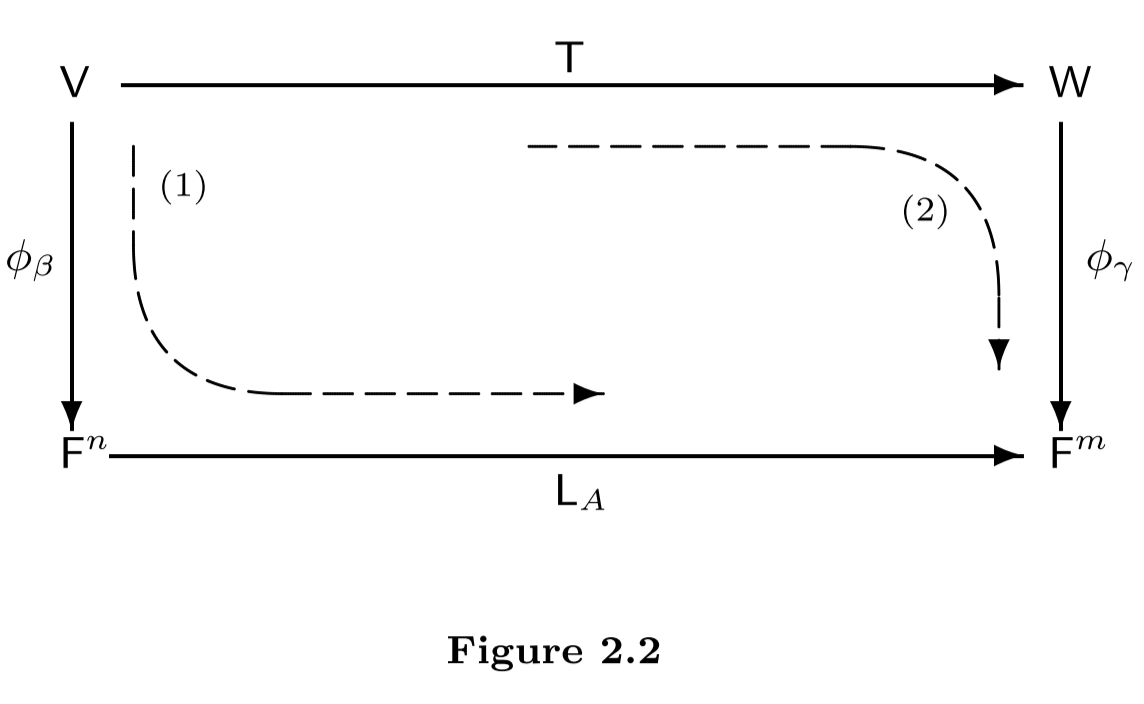
\includegraphics[width=16cm]{images/figure-2-2.png}

Let us first consider Figure 2.2.
Notice that there are two \emph{composites} of \LTRAN{}s that map \(\V\) into \(F^m\):
\begin{enumerate}
\item[1.] Map \(\V\) into \(F^n\) with \(\phi_{\beta}\) and follow this transformation with \(\LMTRAN_A\);
    this yields the composite \(\LMTRAN_A \phi_{\beta}\).
\item[2.] Map \(\V\) into \(\W\) with \(\T\) and follow it by \(\phi_{\gamma}\) to obtain the composite \(\phi_{\gamma} \T\).
\end{enumerate}

\begin{remark} \label{remark 2.4.6}
These two composites are depicted by the dashed arrows in the diagram.
By a simple reformulation of \THM{2.14}, we may conclude that for all \(v \in \V\),
\begin{align*}
    \LMTRAN_A \phi_{\beta}(v)
    & = \LMTRAN_A (\phi_{\beta}(v)) & \text{by def of composition} \\
    & = \LMTRAN_A([v]_{\beta}) & \text{by def of \(\phi_{\beta}\)} \\
    & = A [v]_{\beta} & \text{by def of \(\LMTRAN_A\)} \\
    & = [\T]_{\beta}^{\gamma} [v]_{\beta} & \text{since \(A = [\T]_{\beta}^{\gamma}\)} \\
    & = [\T(v)]_{\gamma} & \text{by \THM{2.14}} \\
    & = \phi_{\gamma}(\T(v)) & \text{by def of \(\phi_{\gamma}\)} \\
    & = \phi_{\gamma} \T (v), & \text{by def of composition}
\end{align*}

Hence \(\LMTRAN_A \phi_{\beta} = \phi_{\gamma} \T\);
that is. the diagram ``commutes.'' (It seems that the terminology is from abstract algebra.)

Heuristically, this relationship indicates that after \(\V\) and \(\W\) are \emph{identified} with \(F^n\) and \(F^m\) via if \(\phi_{\beta}\) and \(\phi_{\gamma}\), respectively,
we may ``identify'' \(\T\) with \(\LMTRAN_A\).
\textbf{This diagram allows us to transfer operations on abstract vector spaces to ones on \(F^n\) and \(F^m\)}.
\end{remark}

\begin{example} \label{example 2.4.7}
Recall the \LTRAN{} \(\T : \POLYRRR \to \POLYRR\) defined in \EXAMPLE{2.2.4} (\(\T(f(x)) = f'(x)\)).
Let \(\beta\) and \(\gamma\) be the standard ordered bases for \(\POLYRRR\) and \(\POLYRR\), respectively,
and let \(\phi_{\beta} : \POLYRRR \to \SET{R}^4\) and \(\phi_{\gamma} : \POLYRR \to \SET{R}^3\) be the corresponding standard representations of \(\POLYRRR\) and \(\POLYRR\).
If \(A = [\T]_{\beta}^{\gamma}\), then
\[
    A = \begin{pmatrix} 0 & 1 & 0 & 0 \\ 0 & 0 & 2 & 0 \\ 0 & 0 & 0 & 3 \end{pmatrix}
\]
Consider the polynomial \(p(x) = 2 + x - 3x^2 + 5x^3\).
We show that \(\LMTRAN_A \phi_{\beta} (p(x)) = \phi_{\gamma} \T (p(x))\).
Now
\[
    \LMTRAN_A \phi_{\beta} (p(x)) = [A]_{\beta}^{\gamma} [p(x)]_{\beta} 
    = \begin{pmatrix} 0 & 1 & 0 & 0 \\ 0 & 0 & 2 & 0 \\ 0 & 0 & 0 & 3 \end{pmatrix} \begin{pmatrix} 2 \\ 1 \\ -3 \\ 5 \end{pmatrix} = \begin{pmatrix} 1 \\ -6 \\ 15 \end{pmatrix}
\]
And since \(\T(p(x)) = p'(x) = 1 - 6x + 15x^2\), we have
\[
    \phi_{\gamma} \T (p(x)) = \phi_{\gamma} (1 - 6x + 15 x^2) = \begin{pmatrix} 1 \\ -6 \\ 15 \end{pmatrix}
\]
So \(\LMTRAN_A \phi_{\beta} (p(x)) = \phi_{\gamma} \T (p(x))\).
\end{example}

\exercisesection

\begin{exercise} \label{exercise 2.4.1}
Label the following statements as true or false.
In each part, \(V\) and \(W\) are vector spaces with ordered (finite) bases \(\alpha\) and \(\beta\), respectively, \(\T: V \to W\) is linear, and \(A\) and \(B\) are matrices.
\begin{enumerate}
\item \(([\T]_{\alpha}^{\beta})^{-1} = [\T^{-1}]_{\alpha}^{\beta}\).
\item \(\T\) is invertible if and only if \(\T\) is one-to-one and onto.
\item \(\T = \LMTRAN_A\), where \(A = [\T]_{\alpha}^{\beta}\).
\item \(M_{2 \X 3}(F)\) is isomorphic to \(F^5\).
\item \(\POLYNF\) is isomorphic to \(\mathcal{P}_m(F)\) if and only if \(n = m\).
\item \(AB = I\) implies that \(A\) and \(B\) are invertible.
\item If \(A\) is invertible, then \((A^{-1})^{-1} = A\).
\item \(A\) is invertible if and only if \(\LMTRAN_A\) is invertible.
\item \(A\) must be square in order to possess an inverse.
\end{enumerate}
\end{exercise}

\begin{proof} \ 

\begin{enumerate}
\item False.
    First, \(\T\) should be invertible to make \(\T^{-1}\) and \(([\T]_{\alpha}^{\beta})^{-1}\) well defined.
    Second, if \(\T\) is invertible, then by \THM{2.18}, \(([\T]_{\alpha}^{\beta})^{-1} = [\T^{-1}]_{\beta}^{\alpha}\).
\item True, this is just true for normal functions.
\item False. the domain and codomain of \(\T\) and \(\LMTRAN_A\) are not necessarily the same.
\item False, \(\dim(M_{2 \X 3}(F)) = 6 \ne 5 = \dim(F^5)\), so by \THM{2.19}, they are not isomorphic to each other.
\item True, \(\POLYNF\) is isomorphic to \(\mathcal{P}_m(F)\), if and only if (by \THM{2.19}) their dimension are equal, that is, if and only if \(n = m\).
\item False, by \DEF{2.13} we also need to check \(BA = I\); and \(A, B\) \emph{must be squares of the same size}.
    Counter example:
    \[
        \left(\begin{array}{lll}
            1 & 0 & 0 \\
            0 & 1 & 0
        \end{array}\right)
        \left(\begin{array}{ll}
            1 & 0 \\
            0 & 1 \\
            0 & 0
        \end{array}\right) = I_2
    \]
\item True.
    If \(A\) is invertible, then by \DEF{2.13}(3) we denote its inverse as \(A^{-1}\);
    in particular by \DEF{2.13}(1) we have \(A A^{-1} = A^{-1} A = I\).
    But this immediately implies \(A^{-1} A = A A^{-1} = I\), so by \DEF{2.13}(1) again, the (unique) inverse of \(A^{-1}\) is \(A\), that is, \((A^{-1})^{-1} = A\).
\item True by \CORO{2.18.2}.
\item True, by \DEF{2.13} (We only define ``invertible'' on square matrix'').
\end{enumerate}
\end{proof}

\begin{exercise} \label{exercise 2.4.2}
For each of the following linear transformations \(\T\), determine whether \(\T\) is invertible and justify your answer.
\begin{enumerate}
\item \(\T : \SET{R}^2 \to \SET{R}^3\) defined by \(\T(a_1, a_2) = (a_1 - 2a_2, a_2, 3a_1 + 4a_2)\).
\item \(\T : \SET{R}^2 \to \SET{R}^3\) defined by \(\T(a_1, a_2) = (3a_1 - a_2, a_2, 4a_1)\).
\item \(\T : \SET{R}^3 \to \SET{R}^3\) defined by \(\T(a_1, a_2, a_3) = (3a_1 - 2a_3, a_2, 3a_1 + 4a_2)\).
\item \(\T : \POLYRRR \to \POLYRR\) defined by \(\T(p(x)) = p'(x)\).
\item \(\T: M_{2 \X 2}(\SET{R}) \to \POLYRR\) defined by \(\T \begin{pmatrix} a & b \\ c & d \end{pmatrix} = a + 2bx + (c + d)x^2\).
\item \(\T : M_{2 \X 2}(\SET{R}) \to M_{2 \X 2}(\SET{R})\) defined by \(\T \begin{pmatrix} a & b \\ c & d \end{pmatrix} = \begin{pmatrix} a + b & a \\ c & c + d \end{pmatrix}\).
\end{enumerate}
\end{exercise}

\begin{proof} \ 

\begin{enumerate}
\item \(\T\) is not invertible since it cannot be an isomorphism by \THM{2.19}.
\item \(\T\) is not invertible since it cannot be an isomorphism by \THM{2.19}.
\item True.
    It's easy to check \(\NULLT = \{ (0, 0, 0) \}\), hence (by \THM{2.4}) \(\T\) is one-to-one (and by \THM{2.5}) is onto;
    and of course \(\T\) is linear, hence (by \RMK{2.4.1}) is invertible.
\item \(\T\) is not invertible since it cannot be an isomorphism by \THM{2.19}.
\item \(\T\) is not invertible since it cannot be an isomorphism by \THM{2.19}.
\item \(\T\) is invertible;
    It's easy to check \(\NULLT = \bigg\{ \begin{pmatrix} 0 & 0 \\ 0 & 0 \end{pmatrix} \bigg\}\), hence \(\T\) is one-to-one, and onto by \THM{2.5};
    and of course \(\T\) is linear.
\end{enumerate}
\end{proof}

\begin{exercise} \label{exercise 2.4.3}
Which of the following pairs of vector spaces are isomorphic?
Justify your answers.
\begin{enumerate}
\item \(F^3\) and \(\mathcal{P}_3(F)\).
\item \(F^4\) and \(\mathcal{P}_3(F)\).
\item \(M_{2 \X 2}(\SET{R})\) and \(\POLYRRR\).
\item \(V = \{ A \in M_{2 \X 2}(\SET{R}) : \TRACE(A) = 0 \}\) and \(\SET{R}^4\).
\end{enumerate}
\end{exercise}

\begin{proof} \ 
\begin{enumerate}
\item \(\dim(F^3) = 3\), \(\dim(\mathcal{P}_3(F)) = 4\), so \(F^3\) and \(\mathcal{P}_3(F)\) are not isomorphic by \THM{2.19}.
\item \(\dim(F^4) = 4\), \(\dim(\mathcal{P}_3(F)) = 4\), so \(F^4\) and \(\mathcal{P}_3(F)\) are isomorphic by \THM{2.19}.
\item \(\dim(M_{2 \X 2}(\SET{R})) = 4\), \(\dim(\mathcal{P}_3(F)) = 4\), so \(M_{2 \X 2}(\SET{R})\) and \(\mathcal{P}_3(F)\) are isomorphic by \THM{2.19}.
\item \(\dim(V) = 2^2 - 1 = 3\) by \ATHM{1.19}(1), \(\dim(\SET{R}^4) = 4\), so \(V\) and \(\SET{R}^4\) are not isomorphic by \THM{2.19}.
\end{enumerate}
\end{proof}

\begin{exercise} \label{exercise 2.4.4}
Let \(A\) and \(B\) be \(n \X n\) invertible matrices.
Prove that \(AB\) is invertible and \((AB)^{-1} = B^{-1}A^{-1}\).
\end{exercise}

\begin{proof}
We have
\begin{align*}
    (AB)(B^{-1}A^{-1}) & = ( A(B B^{-1}) )A^{-1} & \text{by \THM{2.16}, associative} \\
                       & = (A I_n) A^{-1} \\
                       & = A A^{-1} & \text{by \THM{2.12}(c)} \\
                       & = I_n,
\end{align*}
and
\begin{align*}
    (B^{-1}A^{-1})(AB) & = ( B(A A^{-1}) )B^{-1} & \text{by \THM{2.16}, associative} \\
                       & = (B I_n) B^{-1} \\
                       & = B B^{-1} & \text{by \THM{2.12}(c)} \\
                       & = I_n,
\end{align*}
so by \DEF{2.13}, \(AB\) is invertible, and (since the inverse is unique,) \((AB)^{-1} = B^{-1} A^{-1}\).
\end{proof}

\begin{exercise} \label{exercise 2.4.5}
Let \(A\) be invertible.
Prove that \(A^\top\) is invertible and \((A^\top)^{-1} = (A^{-1})^\top\).
\end{exercise}

\begin{note}
The inverse of the transpose of \(A\) is equal to the transpose of the inverse of \(A\), when \(A\) is invertible.
\end{note}

\begin{proof}
We have
\begin{align*}
    A^\top (A^{-1})^\top & = ( A^{-1} A )^\top & \text{by \ATHM{2.24}} \\
                       & = I_n^\top \\
                       & = I_n, & \text{of course}
\end{align*}
and
\begin{align*}
    (A^{-1})^\top A^\top  & = ( A A^{-1} )^\top & \text{by \ATHM{2.24}} \\
                       & = I_n^\top \\
                       & = I_n, & \text{of course}
\end{align*}
so by \DEF{2.13}, \(A^\top\) is invertible, and (since the inverse is unique,) \((A^\top)^{-1} = (A^{-1})^\top\).
\end{proof}

\begin{exercise} \label{exercise 2.4.6}
Prove that if \(A\) is \textbf{invertible} and \(AB = O\), then \(B = O\).
\end{exercise}

\begin{proof}
We have
\begin{align*}
             & AB = O \\
    \implies & A^{-1}(AB) = A^{-1} O = O \\
    \implies & (A^{-1} A)B = O & \text{by \THM{2.16}, associative} \\
    \implies & IB = O \\
    \implies & B = O. & \text{by \THM{2.12}(c)}
\end{align*}
\end{proof}

\begin{exercise} \label{exercise 2.4.7}
Let \(A\) be an \(n \X n\) matrix.
\begin{enumerate}
\item Suppose that \(A^2 = O_{n \X n}\).
    Prove that \(A\) is not invertible.
\item Suppose that \(AB = O_{n \X n}\) for some \textbf{nonzero} \(n \X n\) matrix \(B\).
    Could \(A\) be invertible? Explain.
\end{enumerate}
\end{exercise}

\begin{proof} \ 
\begin{enumerate}
\item For the sake of contradiction, suppose \(A\) is invertible (so we have \(A^{-1}\)).
Then
\begin{align*}
             & A^2 = O_{n \X n} \\
    \implies & A^{-1} (A^2) = A^{-1} O_{n \X n} = O_{n \X n} \\
    \implies & (A^{-1} A) A = O_{n \X n} & \text{by \THM{2.16}, associative} \\
    \implies & IA = O_{n \X n} \\
    \implies & A = O_{n \X n}, & \text{by \THM{2.13}(c)}
\end{align*}
which implies \(A\) is equal to a matrix that is not invertible, a contradiction.
Hence \(A\) is not invertible.

\item
If \(A\) is invertible, then
\begin{align*}
             & AB = O_{n \X n} \\
    \implies & A^{-1} (AB) = A O_{n \X n} = O_{n \X n} \\
    \implies & (A^{-1} A)B = O_{n \X n} & \text{by \THM{2.16}, associative} \\
    \implies & IB = O_{n \X n} \\
    \implies & B = O_{n \X n}, & \text{by \THM{2.13}(c)}
\end{align*}
which contradicts that \(B\) is nonzero.
Hence \(A\) is not invertible.
\end{enumerate}
\end{proof}

\begin{exercise} \label{exercise 2.4.8}
Prove \CORO{2.18.1} and \CORO{2.18.2}.
\end{exercise}

\begin{proof}
See \CORO{2.18.1} and \CORO{2.18.2}.
\end{proof}

\begin{exercise} \label{exercise 2.4.9}
Let \(A\) and \(B\) be \(n \X n\) matrices such that \(AB\) is invertible.
\begin{enumerate}
\item Prove that (\textbf{both}) \(A\) and \(B\) are invertible.
    Hint: See \ATHM{2.26}.
\item Give an example to show that a product of \emph{nonsquare} matrices can be invertible even though the factors, by definition, are not.
\end{enumerate}
\end{exercise}

\begin{note}
By part(b), the supposition that both \(A\) and \(B\) are \(n \X n\) matrix are essential to conclude that they are invertible.
\end{note}

\begin{proof}
Let \(\beta\) be the standard ordered basis for \(F^n\).
Then by \THM{2.15}(a), \([\LMTRAN_A]_{\beta} = A\), \([\LMTRAN_B]_{\beta} = B\), \([\LMTRAN_{AB}]_{\beta} = AB\),
and of course \(\LMTRAN_A, \LMTRAN_B, \LMTRAN_{AB}\) are linear.
\begin{enumerate}
\item Since \(AB\) is invertible, that is, \([\LMTRAN_{AB}]_{\beta}\) is invertible, by \THM{2.18}, \(\LMTRAN_{AB}\) is invertible, that is, by \THM{2.15}(e), \(\LMTRAN_A \LMTRAN_B\) is invertible.
By \ATHM{2.26}(1), \(\LMTRAN_B\) is one-to-one, and by \THM{2.5} (since domain/codomain have the same \(\dim\)), \(\LMTRAN_B\) is onto,
hence \(\LMTRAN_B\) is invertible, hence by \THM{2.18}, \([\LMTRAN_B]_{\beta}\) is invertible, that is, \(B\) is invertible.
Similarly, by \ATHM{2.26}(2), \(\LMTRAN_A\) is onto, and by \THM{2.5} (since domain/codomain have the same \(\dim\)), \(\LMTRAN_A\) is one-to-one,
hence \(\LMTRAN_A\) is invertible, hence by \THM{2.18}, \([\LMTRAN_A]_{\beta}\) is invertible, that is, \(A\) is invertible.

\item
We have
\begin{align*}
    \begin{pmatrix} 1 & 2 & 3 \end{pmatrix}
    \begin{pmatrix} 1 \\ 2 \\ 3 \end{pmatrix}
    = \begin{pmatrix} 10 \end{pmatrix},
\end{align*}
which is an \(1 \X 1\) matrix and has inverse \(( \frac{1}{10} )\).
\end{enumerate}
\end{proof}

\begin{exercise} \label{exercise 2.4.10}
Let \(A\) and \(B\) be \(n \X n\) matrices such that \(AB = I_n\).
\begin{enumerate}
\item Use \EXEC{2.4.9} to conclude that (\textbf{both}) \(A\) and \(B\) are invertible.
\item Prove \(A = B^{-1}\) (and hence \(B = A^{-1}\)).
    (We are, in effect, \textbf{saying that for square matrices, a "one-sided" inverse is a "two-sided" inverse.})
\item State and prove analogous results for linear transformations defined on finite-dimensional vector spaces.
\end{enumerate}
\end{exercise}

\begin{note}
Part(b) says, if \(A, B\) are squares and \(AB = I_n\), then we automatically have \(BA = I_n\), and \(A, B\) are inverse matrices of each other.
\end{note}

\begin{proof} \ 
\begin{enumerate}
\item If \(AB = I_n\), that simply means \(AB\) is invertible, since \(I_n\) is invertible.
So the conditions of \EXEC{2.4.9}(a) are satisfied, hence both \(A, B\) are invertible.

\item We have
\begin{align*}
             & AB = I_n \\
    \implies & A^{-1} (AB) = A^{-1} I_n = A^{-1} & \text{since \(A\) is invertible, and by \THM{2.12}(c)} \\
    \implies & (A^{-1}A)B = A^{-1} & \text{by \THM{2.16}, associative} \\
    \implies & I_n B = A^{-1} \\
    \implies & B = A^{-1}. & \text{by \THM{2.12}(c)}
\end{align*}
And by \DEF{2.13}, this implies \(AB = BA = I_n\).
In particular, we have \(BA = AB = I_n\), so by \DEF{2.13} again, \(B^{-1} = A\).

\item
Statement: Let \(\T : V \to W\) and \(\U : W \to V\) where \(V, W\) have same (finite) dimensions and \(\U\T = \ITRANV\).
Then both \(\U, \T\) are invertible. and we have \((\T)^{-1} = \U\) (hence \(\U^{-1} = \T\)).

First, similar to \EXEC{2.4.9}, by \ATHM{2.26}(1)(2), both \(\U, \T\) are invertible.
And (by general version of \THM{2.10},) we have
\begin{align*}
             & \U\T = \ITRANV \\
    \implies & \U^{-1} (\U\T) = \U^{-1} \ITRANV = \U^{-1} & \text{since \(\U\) is invertible, and by \THM{2.10}(c)} \\
    \implies & (\U^{-1}\U)\T = \U^{-1} & \text{by \THM{2.10}(b), associative} \\
    \implies & \ITRANW \T = \U^{-1} \\
    \implies & \T = \U^{-1}. & \text{by \THM{2.10}(c)}
\end{align*}
And by \DEF{2.12}, this implies \(\U\T = \ITRANV\) and \(\T\U = \ITRANW\).
In particular, we have \(\T\U = \ITRANW\) and \(\U\T = \ITRANV\) and, so by \DEF{2.12} again, \(\T^{-1} = \U\).
\end{enumerate}
\end{proof}

\begin{exercise} \label{exercise 2.4.11}
Verify that the transformation in \EXAMPLE{2.4.5} is one-to-one.
\end{exercise}

\begin{proof}
Suppose \(f \in \NULLT\), we have to show \(f\) is zero polynomial to show \(\T\) is one-to-one.
Then we have \(f(1) = f(2) = f(3) = f(4) = 0\).
But by \RMK{1.6.6} we know that \(f\) is the zero polynomial, as desired.
\end{proof}

\begin{exercise} \label{exercise 2.4.12}
Prove \THM{2.21}.
\end{exercise}

\begin{proof}
See \THM{2.21}.
\end{proof}

\begin{exercise} \label{exercise 2.4.13}
Let \(\sim\) mean ``is isomorphic to.'' (\DEF{2.14})
Prove that \(\sim\) is an equivalence relation on the class of vector spaces over \(F\).
\end{exercise}

\begin{proof}\ 

Reflexivity: \(V\) is isomorphic to \(V\) since \(\ITRANV\) is an isomorphism from \(V\) to \(V\) for any vector space \(V\).

Symmetry: Suppose \(V\) is isomorphic to \(W\), then there exists an isomorphism \(\T\) from \(V\) to \(W\).
In particular, by \DEF{2.14}, \(\T\) is invertible, so \(\T^{-1} : W \to V\) exists, and also invertible.
And by \THM{2.17}, \(\T^{-1}\) is linear.
Hence by \DEF{2.14} again, \(\T^{-1}\) is an isomorphism from \(W\) to \(V\).
Hence \(W\) is isomorphic to \(V\).

Transitivity: Suppose \(V\) is isomorphic to \(W\) and \(W\) is isomorphic to \(Z\), then there exists an isomorphism \(\T\) from \(V\) to \(W\) and \(\U\) from \(W\) to \(Z\).
Furthermore, by \ATHM{2.26}(c) \(\U\T\) is invertible, and by \THM{2.9}, since \(\U, \T\) are linear, \(\U\T\) is also linear, hence \(\U\T\) is an isomorphism by \DEF{2.14}.
Hence \(V\) is isomorphic to \(Z\).
\end{proof}

\begin{exercise} \label{exercise 2.4.14}
Let
\[
    V = \bigg\{ \begin{pmatrix} a & a + b \\ 0 & c \end{pmatrix} : a, b, c \in F \bigg\}.
\]
Construct an isomorphism from \(V\) to \(F^3\).
\end{exercise}

\begin{proof}
Clearly,
\[\beta = \bigg\{
    \begin{pmatrix} 1 & 0 \\ 0 & 0 \end{pmatrix},
    \begin{pmatrix} 0 & 1 \\ 0 & 0 \end{pmatrix},
    \begin{pmatrix} 0 & 0 \\ 0 & 1 \end{pmatrix}
\bigg\}\]
is a basis for \(V\).
Then by \THM{2.21}, \(\phi_{\beta}\) is an isomorphism from \(V\) to \(F^3\).
\end{proof}

\begin{exercise} \label{exercise 2.4.15}
Let \(V\) and \(W\) be \(n\)-dimensional vector spaces, and let \(\T : V \to W\) be a linear transformation.
Suppose that \(\beta\) is a basis for \(V\).
Prove that \(\T\) is an isomorphism \emph{if and only if} \(\T(\beta)\) is a basis for \(W\).
\end{exercise}

\begin{proof} \ 

\(\Longrightarrow\): Suppose \(\T\) is an isomorphism.
In particular, \(\T\) is one-to-one and onto.
Then by \ATHM{2.2}(2.c), \(\T(\beta)\) is a basis for \(W\).

\(\Longleftarrow\): Suppose \(\T(\beta)\) is a basis for \(W\).
In particular, \(\spann(\T(\beta)) = W\).
And by \THM{2.2}, \(\RANGET = \spann(\T(\beta)) = W\), hence \(\T\) is onto.
By \THM{2.5}, \(\T\) is one-to-one.
Hence \(\T\) is an isomorphism.
\end{proof}

\begin{exercise} \label{exercise 2.4.16}
Let \(B\) be an \(n \X n\) \emph{invertible} matrix.
Define \(\Phi : M_{n \X n}(F) \to M_{n \X n}(F)\) by \(\Phi(A) = B^{-1}AB\).
Prove that \(\Phi\) is an isomorphism.
\end{exercise}

\begin{note}
This is called ``matrix similarity''; we say that \(\Phi(A)\)(or \(B^{-1}AB\)) and \(A\) are similar.
This concept is introduced in the next section(\DEF{2.16}) and is used in \CH{5}.
\end{note}

\begin{proof}
First, it's trivial that \(\Phi\) is linear since it only involves matrix multiplication and you can use \THM{2.10} to check linearity.
Now to show that \(\Phi\) is invertible, since domain/codomain have the same dimensions, we only need to show \(\Phi\) is onto.
But given \(D \in M_{n \X n}(F)\), we have \(B D B^{-1} \in M_{n \X n}(F)\) such that
\begin{align*}
    \Phi(B D B^{-1}) & = B^{-1} (B D B^{-1}) B & \text{by def of \(\Phi\)} \\
                     & = (B^{-1}B) D (B^{-1} B) & \text{of course} \\
                     & = IDI & \text{of course} \\
                     & = D & \text{of course}
\end{align*}
So \(\Phi\) is onto, as desired.
\end{proof}

\begin{exercise} \label{exercise 2.4.17}
Let \(V\) and \(W\) be finite-dimensional vector spaces and \(\T : V \to W\) be an isomorphism.
Let \(V_0\) be a \emph{subspace} of \(V\).
\begin{enumerate}
\item Prove that \(\T(V_0)\) is a subspace of \(W\).
\item Prove that \(\dim(V_0) = \dim(\T(V_0))\).
\end{enumerate}
And from part(b), we say that an isomorphism is \emph{rank-preserving}, since in particular \(\dim(V) = \dim(\T(V))\).
\end{exercise}

\begin{proof} \ 

\begin{enumerate}
\item It is true by \ATHM{2.4}(1).
\item By \THM{2.19}, it suffices to show that \(V_0\) and \(\T(V_0)\) are isomorphic.
And we claim that \(\T' : V_0 \to \T(V_0)\) by \(\T'(v) = \T(v)\) for \(v \in V_0\) is an isomorphism from \(V_0\) to \(\T(V_0)\).

First, of course \(\T'\) is linear.
For one-to-one, given \(v_1, v_2 \in V_0\),
\begin{align*}
             & \T'(v_1) = \T'(v_2) \\
    \implies & \T(v_1) = \T(v_2) & \text{by def of \(\T'\)} \\
    \implies & v_1 = v_2. & \text{since in particular \(\T\) is one-to-one}
\end{align*}

For onto, given \(w \in \T(V_0)\), then by definition of \(\T(V_0)\) we of course can find \(v \in V_0\) such that \(\T(v) = W\).
But since \(v \in V_0\), \(\T'(v) = \T(v)\).
Hence we have found \(v \in V_0\) such that \(\T'(v) = w\), so \(\T'\) is onto.

So \(\T'\) is an isomorphism from \(V_0\) to \(\T(V_0)\), as desired.
\end{enumerate}

\end{proof}

\begin{exercise} \label{exercise 2.4.18}
Repeat \EXAMPLE{2.4.7} with the polynomial \(p(x) = 1 + x + 2x^2 + x^3\).
\end{exercise}

\begin{proof}
Let 
\[
    A = [\T]_{\beta}^{\gamma} = \begin{pmatrix} 0 & 1 & 0 & 0 \\ 0 & 0 & 2 & 0 \\ 0 & 0 & 0 & 3 \end{pmatrix}
\]
We show that \(\LMTRAN_A \phi_{\beta} (p(x)) = \phi_{\gamma} \T (p(x))\).
Now
\[
    \LMTRAN_A \phi_{\beta} (p(x)) = [A]_{\beta}^{\gamma} [p(x)]_{\beta} 
    = \begin{pmatrix} 0 & 1 & 0 & 0 \\ 0 & 0 & 2 & 0 \\ 0 & 0 & 0 & 3 \end{pmatrix} \begin{pmatrix} 1 \\ 1 \\ 2 \\ 1 \end{pmatrix} = \begin{pmatrix} 1 \\ 4 \\ 3 \end{pmatrix}
\]
But since \(\T(p(x)) = p'(x) = 1 + 4x + 3x^2\), we have
\[
    \phi_{\gamma} \T (p(x)) = \phi_{\gamma} (1 + 4x + 3x^2) = \begin{pmatrix} 1 \\ 4 \\ 3 \end{pmatrix}
\]
So \(\LMTRAN_A \phi_{\beta} (p(x)) = \phi_{\gamma} \T (p(x))\).
\end{proof}

\begin{exercise} \label{exercise 2.4.19}
In \EXAMPLE{2.1.5}, the mapping \(\T : M_{2 \X 2}(\SET{R}) \to M_{2 \X 2}(\SET{R})\) defined by \(\T(M) = M^\top\) for each \(M \in M_{2 \X 2}(\SET{R})\) is a linear transformation.
Let \(\beta = \{ E_{11}, E_{12}, E_{21}, E_{22} \}\), which is a basis for \(M_{2 \X 2}(\SET{R})\), as noted in \EXAMPLE{1.6.3}.
\begin{enumerate}
\item Compute \([\T]_{\beta}\).
\item Verify that \(\LMTRAN_A \phi_{\beta} (M) = \phi_{\beta} \T(M)\) for \(A = [\T]_{\beta}\) and \(M = \begin{pmatrix} 1 & 2 \\ 3 & 4 \end{pmatrix}\).
\end{enumerate}
\end{exercise}

\begin{proof} \ 

\begin{enumerate}
\item From \EXEC{2.2.5}(a),
\[
    [\T]_{\beta}
    = \begin{pmatrix}
        \MAROON{1} & \BLUE{0} & \RED{0} & \GREEN{0} \\
        \MAROON{0} & \BLUE{0} & \RED{1} & \GREEN{0} \\
        \MAROON{0} & \BLUE{1} & \RED{0} & \GREEN{0} \\
        \MAROON{0} & \BLUE{0} & \RED{0} & \GREEN{1}
    \end{pmatrix}
\]

\item
\[
    \LMTRAN_A \phi_{\beta}(M) = 
    = \begin{pmatrix}
        1 & 0 & 0 & 0 \\
        0 & 0 & 1 & 0 \\
        0 & 1 & 0 & 1 \\
        0 & 0 & 0 & 1
    \end{pmatrix}
    \begin{pmatrix} 1 \\ 2 \\ 3 \\4 \end{pmatrix}
    = \begin{pmatrix} 1 \\ 3 \\ 2 \\ 4 \end{pmatrix}
\]
and
\[
    \phi_{\beta}\T(M)
    = \phi_{\beta}\begin{pmatrix} 1 & 3 \\ 2 & 4 \end{pmatrix}
    = \begin{pmatrix} 1 \\ 3 \\ 2 \\ 4 \end{pmatrix}
\]
So \(\LMTRAN_A \phi_{\beta}(M) = \phi_{\beta}\T(M)\).
\end{enumerate}
\end{proof}

\begin{exercise} \label{exercise 2.4.20}
Let \(\T: V \to W\) be a \LTRAN{} from an \(n\)-dimensional vector space \(V\) to an \(m\)-dimensional vector space \(W\).
Let \(\beta\) and \(\gamma\) be ordered bases for \(V\) and \(W\), respectively.
Prove that \(\rankT = \rank(\LMTRAN_A)\) and that \(\nullityT = \nullity(\LMTRAN_A)\), where \(A = [\T]_{\beta}^{\gamma}\).
Hint: Apply \EXEC{2.4.17} to Figure 2.2.
\end{exercise}

\begin{proof} \ 

\(\rankT = \rank(\LMTRAN_A)\):
Since \(\LMTRAN_A \phi_{\beta} = \phi_{\gamma} \T \), in particular we have \(\LMTRAN_A \phi_{\beta}(V) = \phi_{\gamma} \T(V)\) \MAROON{(1)}.

Now, for the dimension of RHS of \MAROON{(1)},
\begin{align*}
    & \dim(\phi_{\gamma} \T(V)) \\
    & = \dim(\phi_{\gamma} (\T(V))) & \text{by def of composition} \\
    & = \dim(\T(V)) & \text{since \(\phi_{\gamma}\) is an isomorphism, and by \EXEC{2.4.17}(b)} \\
    & = \rankT, & \text{by definition}
\end{align*}
and for the dimension of LHS of \MAROON{(1)},
\begin{align*}
    & \dim(\LMTRAN_A \phi_{\beta}(V)) \\
    & = \dim(\LMTRAN_A (\phi_{\beta}(V))) & \text{by def of composition} \\
    & = \dim(\LMTRAN_A (F^n)) & \text{since (in particular) \(\phi_{\beta}\) is onto} \\
    & = \dim(\RANGE(\LMTRAN_A)) & \text{by definition} \\
    & = \rank(\LMTRAN_A), & \text{by definition}
\end{align*}
Hence we have \(\rankT = \rank(\LMTRAN_A)\), as desired.

\(\nullityT = \nullity(\LMTRAN_A)\):
We have
\begin{align*}
    \nullityT & = \dim(V) - \rankT & \text{by \THM{2.3}(dimension theorem)} \\
              & = \dim(F^n) - \rankT & \text{of course, since \(\dim(V) = n\)} \\
              & = \dim(F^n) - \rank(\LMTRAN_A) & \text{by what we have shown} \\
              & = \nullity(\LMTRAN_A). & \text{again by \THM{2.3}}
\end{align*}
\end{proof}

\begin{exercise} \label{exercise 2.4.21}
Let \(V\) and \(W\) be \emph{finite}-dimensional vector spaces with ordered bases \(\beta = \{ v_1, v_2, ..., v_n \}\) and \(\gamma = \{ w_1, w_2, ..., w_m \}\), respectively.
By \THM{2.6}, there exist unique linear transformations \(\T_{ij} : V \to W\) such that
\begin{equation*}
    \T_{ij}(v_k) = \begin{cases}
        w_i, \text{ if } k = j \\
        \OW, \text{ if } k \ne j
    \end{cases}
\end{equation*}
First prove that \(\alpha = \{ T_{ij} : 1 \le i \le m, 1 \le j \le n \}\) is a basis for \(\mathcal{L}(V, W)\).
Then let \(M^{ij}\) be the \(m \X n\) matrix with \(1\) in the \(i\)th row and \(j\)th column and \(0\) elsewhere, and prove that \([\T_{ij}]_{\beta}^{\gamma} = M^{ij}\).
Again by \THM{2.6}, there exists a unique linear transformation \(\Phi_{\beta}^{\gamma} : \mathcal{L}(V, W) \to M_{m \X n}(F)\) such that \(\Phi_{\beta}^{\gamma} (\T_{ij}) = M^{ij}\).
Prove that \(\Phi_{\beta}^{\gamma}\) is an isomorphism.
\end{exercise}

\begin{proof}
Since \(\#\alpha = \dim(\mathcal{L}(V, W)\) (where by \THM{2.20} we can conclude \(\dim(\mathcal{L}(V, W) = mn\)), (by \CORO{1.10.3}(b)) we only need to show \(\alpha\) is \LID{}.
BTW, we use the symbol \(\TZERO\) to represent the zero vector, i.e. the zero transformation, of \(\mathcal{L}(V, W)\).

So suppose \(\sum_{i = 1}^{m} \sum_{j = 1}^n a_{ij} \T_{ij} = \TZERO\) \MAROON{(1)}, we have to show \(a_{ij} = 0\) for all \(1 \le i \le m\), \(1 \le j \le n\).
But given arbitrary \(k\) such that \(1 \le k \le n\),
\begin{align*}
    \OW & = \TZERO(v_k) & \text{of course} \\
        & = \bigg( \sum_{i = 1}^{m} \sum_{j = 1}^n a_{ij} \T_{ij} \bigg) (v_k) & \text{by \MAROON{(1)}} \\
        & = \sum_{i = 1}^{m} \sum_{j = 1}^n a_{ij} \T_{ij} (v_k) & \text{by def of \(+\) and scalar \(\cdot\) of functions} \\
        & = \sum_{i = 1}^{m} \bigg( a_{i1} \T_{i1} (v_k) + a_{i2} \T_{i2} (v_k) + ... + a_{in} \T_{in} (v_k) \bigg) & \text{expanding summation} \\
        & = \sum_{i = 1}^{m} \bigg( a_{i1} \OV + ... + a_{ik} w_i + ... + a_{in} \OV \bigg) & \text{by definition of \(\T_{ij}\)} \\
        & = \sum_{i = 1}^m a_{ik} w_i,
\end{align*}
which implies \(a_{1k} = a_{2k} = ... = a_{mk} = 0\) since \(\gamma\) is a basis for \(W\).
Since \(k\) is arbitrary, we have \(a_{ik} = 1\) for all \(1 \le i \le m\), \(1 \le k \le n\), as desired.

Now given arbitrary \(j\) such that \(1 \le j \le n\), it trivial that the \(j\)th column of \(M^{ij}\) is \(e_i\) where \(e_i\) is the \(i\)th standard vector of \(F^m\).
And by definition, the \(j\)th column of \([\T_{ij}]_{\beta}^{\gamma}\) is \([\T_{ij}(v_j)]_{\gamma}\), but
\begin{align*}
    [\T_{ij}(v_j)]_{\gamma} & = [w_i]_{\gamma} & \text{by definition of \(T^{ij}\)} \\
                 & = e_i & \text{of course}
\end{align*}
Hence \(M^{ij} = [\T_{ij}]_{\gamma}\).

Finally, And since \(\alpha' = \{ M_{ij} : 1 \le i \le m, 1 \le j \le n \}\) is a basis for \(M_{m \X n}(F)\), and \(\Phi_{\beta}^{\gamma}(\alpha) = \alpha'\), by \EXEC{2.4.15}, \(\Phi_{\beta}^{\gamma}\) is an isomorphism.
\end{proof}

\begin{exercise} \label{exercise 2.4.22}
Let \(c_0, c_1, ..., c_n\) be \emph{distinct} scalars from an infinite field \(F\).
Define \(\T: \POLYNF \to F^{n + 1}\) by \(\T(f) = (f(c_0), f(c_1), ..., f(c_n))\).
Prove that \(\T\) is an isomorphism.
Hint: Use the Lagrange polynomials associated with \(c_0, c_1, ..., c_n\).
\end{exercise}

\begin{proof}
(This exercise is similar to \EXEC{2.4.11}.)
First it's of course that \(\T\) is linear.
And since \(\dim(\POLYNF) = \dim(F^{n + 1})\), we only have to show \(\T\) is one-to-one.
So suppose \(f \in \NULLT\), we have to show \(f\) is zero polynomial to show \(\T\) is one-to-one.
Then we have \(\T(f) = (f(c_0), f(c_1), ..., f(c_n)) = (0, 0, ..., 0)\).
But by \RMK{1.6.6}, we know that \(f\) is zero polynomial, as desired.
\end{proof}

\begin{exercise} \label{exercise 2.4.23}
Let \(W\) denote the vector space of all \emph{sequences} in \(F\) that \emph{have only a finite number of nonzero terms} (defined in \EXEC{1.6.18}),
and let \(Z = \POLYF\).
Define
\[
    \T : W \to Z \text{ by } \T(\sigma) = \sum_{i = 0}^n \sigma(i)x^i,
\]
where \(n\) is the \emph{largest integer} such that \(\sigma(n) \ne 0\). Prove that \(\T\) is an isomorphism.
\end{exercise}

\begin{proof}
Since the domain and codomain of \(\T\) are infinite-dimensional, we need to show that \(\T\) is linear, one-to-one, onto, respectively.

First, given \(\sigma_1, \sigma_2 \in W\) and scalar \(c \in F\), where \(n_1\), \(n_2\) are the largest nonzero integers such that \(\sigma_1(n_1) \ne 0\) and \(\sigma_2(n_2) \ne 0\), respectively.
Then
\begin{align*}
    & \T(\sigma_1 + c \sigma_2) \\
    & = \sum_{i = 0}^{\max(n_1, n_2)} (\sigma_1 + c \sigma_2)(i) x^i & \text{by def of \(\T\)} \\
    & = \sum_{i = 0}^{\max(n_1, n_2)} (\sigma_1(i) + c \sigma_2(i)) x^i & \text{by def of \(+\) and scalar \(\cdot\) of functions} \\
    & = \sum_{i = 0}^{\max(n_1, n_2)} \sigma_1(i) x^i + c \sigma_2(i) x^i & \text{of course} \\
    & = \sum_{i = 0}^{\max(n_1, n_2)} \sigma_1(i) x^i + c \sum_{i = 0}^{\max(n_1, n_2)} \sigma_2(i) x^i & \text{by splitting summation and move constant} \\
    & = \sum_{i = 0}^{n_1} \sigma_1(i) x^i + c \sum_{i = 0}^{n_2} \sigma_2(i) x^i & \text{of course} \\
    & = \T(\sigma_1) + c\T(\sigma_2), & \text{by def of \(\T\)}
\end{align*}
hence by \ATHM{2.1}(b), \(\T\) is linear.

Now, by the property of polynomial, it's really clear that \(\T\) is one-to-one (only zero sequence gives zero polynomial) and onto (every polynomial can be represented as a sequence of finite nonzero terms), hence \(\T\) is an isomorphism.
\end{proof}

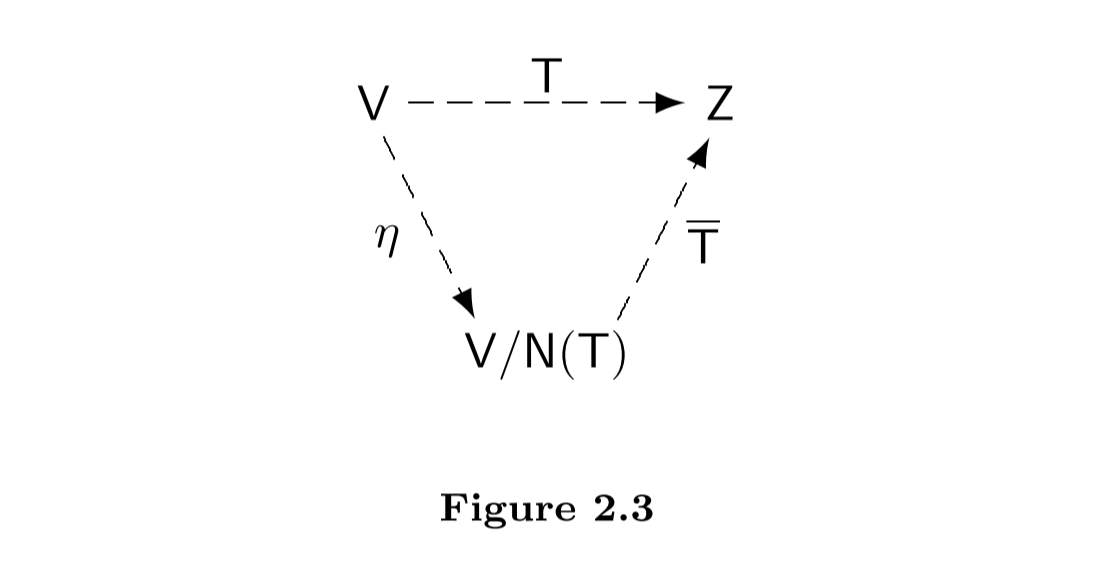
\includegraphics[width=16cm]{images/figure-2-3.png}

\begin{exercise} \label{exercise 2.4.24}
Let \(V\) and \(Z\) be vector spaces and \(\T : V \to Z\) be a linear transformation \emph{that is onto}.
Define the mapping
\[
    \overline{\T} : V / \NULLT \to Z \text{ by } \overline{\T}(v + \NULLT) = \T(v)
\]
for any coset \(v + \NULLT\) in \(V / \NULLT\).
\begin{enumerate}
\item Prove that \(\overline{\T}\) is \emph{well-defined};
    that is, prove that if \(v + \NULLT = v' + \NULLT\), then \(\T(v) = \T(v')\).
\item Prove that \(\overline{\T}\) is linear.
\item Prove that \(\overline{\T}\) is an isomorphism.
\item Prove that the diagram shown in Figure 2.3 \emph{commutes};
    that is, prove that \(\T = \overline{\T} \eta\). (\(\eta\) is defined in \EXEC{2.1.42}.)
\end{enumerate}

Note that we do not say \(V\) and \(Z\) are finite dimensional.
\end{exercise}

\begin{proof} \ 

\begin{enumerate}
\item Suppose \(v + \NULLT = v' + \NULLT\), then by \ATHM{1.10}(b), \(v - v' \in \NULLT\), which implies \(\T(v - v') = 0_{_Z}\), that is, \(\T(v) - \T(v') = 0_{_Z}\), that is, \(\T(v) = \T(v')\).

\item For any \(v_1 + \NULLT\) and \(v_2 + \NULLT\) in \(V/\NULLT\), and any scalar \(c\),
\begin{align*}
    & \overline{\T}\bigg( \big( v_1 + \NULLT \big) + c \big(v_2 + \NULLT \big)  \bigg) \\
    & = \overline{\T}\big( (v_1 + cv_2) + \NULLT) \big) & \text{by def of coset \(+\) and scalar \(\cdot\), see \EXEC{1.3.31}} \\
    & = \T(v_1 + cv_2) & \text{by def of \(\overline{\T}\)} \\
    & = \T(v_1) + c\T(v_2) & \text{since \(\T\) is linear} \\
    & = \overline{\T}(v_1 + \NULLT) + c\overline{\T}(v_2 + \NULLT), & \text{by def of \(\overline{\T}\)}
\end{align*}
hence by \ATHM{2.1}(b), \(\overline{\T}\) is linear.

\item Now we have to show \(\overline{\T}\) is one-to-one and onto.
For one-to-one, suppose \(v + \NULLT \in \NULL(\overline{\T})\), we have to show \(v + \NULLT = \OV + \NULLT\).
Then by definition of \(\overline{\T}\), \(\overline{\T}(v + \NULLT) = \T(v) = 0_{_Z}\), which implies \(v \in \NULLT\).
And of course \(v - \OV \in \NULLT\), so by \ATHM{1.10}(b), \(v + \NULLT = \OV + \NULLT\), as desired.

For onto, suppose arbitrary \(z \in Z\).
\emph{Then since \(\T\) is onto}, we can find \(v \in V\) such that \(\T(v) = z\), and for such \(v\) of course we can find \(v + \NULLT \in V/\NULLT\) such that \(\overline{\T}(v + \NULLT) = \T(v) = z\).
Hence \(\overline{\T}\) is onto.

Hence \(\overline{\T}\) is an isomorphism from \(V/\NULLT\) to \(Z\).

\item It's somewhat ambiguous that the exercise does not mention the corresponding \(W\) of the linear map \(\eta\).
Anyway, we assume \(\eta : V \to V/\NULLT\) by \(\eta(v) = v + \NULLT\).
Then for all \(v \in V\), we have
\begin{align*}
    \overline{\T}\eta(v) & = \overline{\T}(\eta(v)) & \text{by def of composition} \\
                         & = \overline{\T}(v + \NULLT) & \text{by def of \(\eta\)} \\
                         & = \T(v) & \text{by def of \(\overline{\T}\)}
\end{align*}
Hence \(\T = \overline{\T}\eta\).
\end{enumerate}
\end{proof}

\begin{exercise} \label{exercise 2.4.25}
\TODOREF{} \RED{Skip}, this need section 1.7.
\end{exercise}

\begin{proof}
\end{proof}

\begin{additional theorem} \label{athm 2.36}
This is the placeholder theorem for some matrix inversion equations:

\BLUE{(1)} \EXEC{2.4.4}: \((AB)^{-1} = B^{-1} A^{-1}\) when \(A, B\) are invertible (and compatible).

\BLUE{(2)} \EXEC{2.4.5}: \((A^\top)^{-1} = (A^{-1})^\top\) when \(A\) is invertible.
\end{additional theorem}

\begin{additional theorem} \label{athm 2.37}
This is the placeholder theorem for some judgement of zero matrix and invertibility:

\BLUE{(1)} \EXEC{2.4.6}: If \(A\) is invertible and \(AB = O\), then \(B = O\).

\EXEC{2.4.7}:

\BLUE{(2.1)}: If \(A^2 = O\) then \(A\) is not invertible.

\BLUE{(2.2)}: If \(AB = O\) for some \emph{nonzero} \(n \X n\) matrix \(B\), then \(A\) is not invertible.

\BLUE{(3)} \EXEC{2.4.9}: If \(A\) and \(B\) be \(n \X n\) matrices such that \(AB\) is invertible, then both \(A\) and \(B\) are invertible.
\end{additional theorem}

\begin{additional theorem} \label{athm 2.38}
This is the placeholder theorem for \EXEC{2.4.10}:

\BLUE{(1)}: If \(A, B\) are \(n \X n\) squares and \(AB = I_n\), then \(A, B\) are invertible, and \(A = B^{-1}\) and \(B = A^{-1}\).
In fact, we do not need to check \(BA = I_n\), hence a ``one-sided'' inverse is a ``two-sided'' inverse.

\BLUE{(2)}: Analogous result for \LTRAN{}:
Let \(\T : V \to W\) and \(\U : W \to V\) where \(V, W\) have same (finite) dimensions and \(\U\T = \ITRANV\).
Then both \(\U, \T\) are invertible. and we have \((\T)^{-1} = \U\) (hence \(\U^{-1} = \T\)).
\end{additional theorem}

\begin{additional theorem} \label{athm 2.39}
This is the placeholder theorem for \EXEC{2.4.15}:
If \(\T : V \to W\) is a \LTRAN{}, and \(\beta\) is a basis for \(V\), then \(\T\) is an isomorphism (from \(V\) to \(W\)) if and only if \(\T(\beta)\) is a basis for \(W\).
\end{additional theorem}

\begin{additional theorem} \label{athm 2.40}
This is the placeholder theorem for \EXEC{2.4.16}:
Given \(n \X n\) invertible matrix \(B\),
\(\Phi : M_{n \X n}(F) \to M_{n \X n}(F)\) by \(\Phi(A) = B^{-1}AB\) is an isomorphism.
\end{additional theorem}

\begin{additional theorem} \label{athm 2.41}
This is the placeholder theorem for \EXEC{2.4.17}:
Let \(V\) and \(W\) be finite-dimensional vector spaces and \(\T : V \to W\) be an isomorphism.
Let \(V_0\) be a \emph{subspace} of \(V\).
Then

\BLUE{(1)} \(\T(V_0)\) is a subspace of \(W\), and

\BLUE{(2)} \(\dim(V_0) = \dim(\T(V_0))\);
    we say that an isomorphism is \emph{rank-preserving}, since in particular \(\dim(V) = \dim(\T(V))\).
\end{additional theorem}

\begin{additional theorem} \label{athm 2.42}
This is the placeholder theorem for \EXEC{2.4.20}:
Let \(\T: V \to W\) be a linear transformation from an \(n\)-dimensional vector space \(V\) to an \(m\)-dimensional vector space \(W\).
Let \(\beta\) and \(\gamma\) be ordered bases for \(V\) and \(W\), respectively.
Then \(\rankT = \rank(\LMTRAN_A)\) and that \(\nullityT = \nullity(\LMTRAN_A)\), where \(A = [\T]_{\beta}^{\gamma}\).
\end{additional theorem}

\begin{additional theorem} \label{athm 2.43}
This is the placeholder theorem for \EXEC{2.4.21}, which gives an isomorphism \(\Phi_{\beta}^{\gamma} : \mathcal{L}(V, W) \to M_{m \X n}(F)\).
\end{additional theorem}

\begin{additional theorem} \label{athm 2.44}
This is the placeholder theorem for \EXEC{2.4.22}, which gives an isomorphism from \(\POLYNF\) to \(F^{n + 1}\);
And this isomorphism is related to Lagrange polynomials(or \RMK{1.6.6}).
\end{additional theorem}

\begin{additional theorem} \label{athm 2.45}
This is the placeholder theorem for \EXEC{2.4.24}, which gives some other facts about quotient space.
\end{additional theorem}
\section{The Change of Coordinate Matrix} \label{sec 2.5}

\begin{note}
Some of inverse matrices in the examples are (mysteriously) given, but in fact currently we do not know how to calculate the inverse of a invertible matrix.
This is introduced in \CH{3}.
\end{note}

In many areas of mathematics, a \emph{change of variable} is used to \emph{simplify the appearance} of an expression.
For example, in geometry the change of variable
\[
    \begin{array}{l}
        x=\frac{2}{\sqrt{5}} x^{\prime}-\frac{1}{\sqrt{5}} y^{\prime} \\
        y=\frac{1}{\sqrt{5}} x^{\prime}+\frac{2}{\sqrt{5}} y^{\prime}
\end{array}
\]
can be used to transform the equation \(2x^2 - 4xy + 5y^2 = 1\) into the simpler equation \((x')^2 + 6(y')^2 = 1\), a \emph{form} in which it is easily seen to be the equation of an ellipse. (See Figure 2.4.)

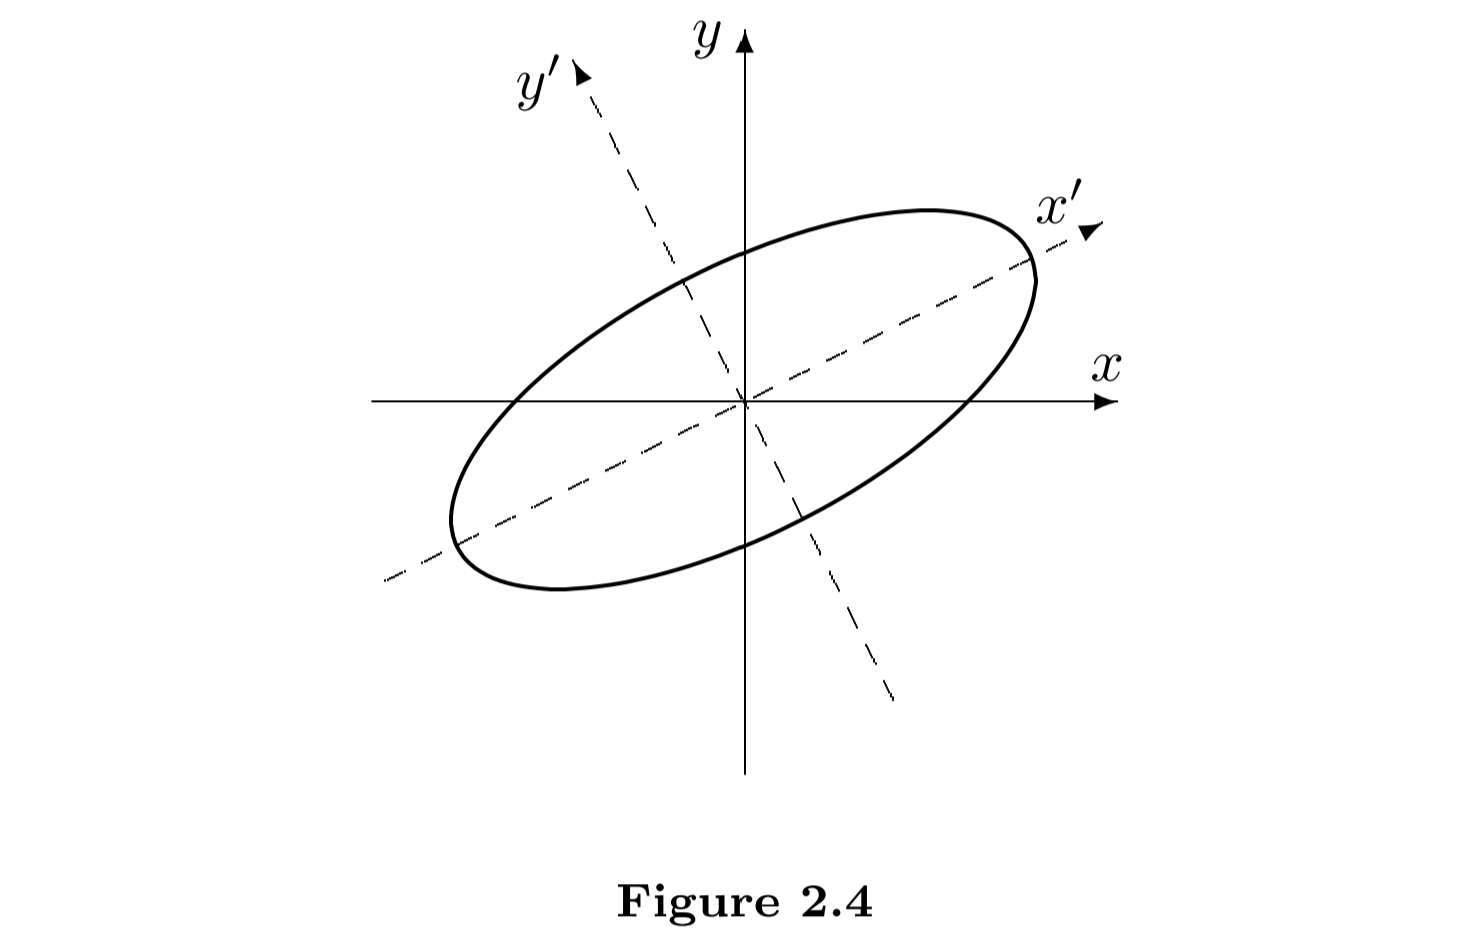
\includegraphics[width=10cm]{images/figure-2-4.png}

We will see how this change of variable is \emph{determined} in \SEC{6.5}.

(For figure 2.4,) Geometrically, the change of variable
\[
    P = \begin{pmatrix} x \\ y \end{pmatrix} \to \begin{pmatrix} x' \\ y' \end{pmatrix}
\]
is a \emph{change in the way} that the position of a point \(P\) in the plane is \emph{described}.
This is done by \emph{introducing a new frame of reference}, an \(x'y'\)-coordinate system with coordinate axes \emph{rotated} from the original \(xy\)-coordinate axes.
In this case, the new coordinate axes(\(x'\)-axis and \(y'\)-axis) are chosen to \emph{lie in the direction of the axes} of the ellipse.
The \textbf{unit vectors} along the \(x'\)-axis and the \(y'\)-axis form an \emph{ordered basis} for \(\SET{R}^2\):
\[
    \beta' = \bigg\{ \frac{1}{\sqrt{5}} \begin{pmatrix} 2 \\ 1 \end{pmatrix}, \frac{1}{\sqrt{5}} \begin{pmatrix} -1 \\ 2 \end{pmatrix} \bigg\}
\]
and the change of variable is actually a change from \([P]_{\beta} = \begin{pmatrix} x \\ y \end{pmatrix}\), the coordinate vector of \(P\) relative to the \emph{standard} ordered basis \(\beta = \{ e_1, e_2 \}\), to \([P]_{\beta'} = \begin{pmatrix} x' \\ y' \end{pmatrix}\), the coordinate vector of \(P\) relative to the new rotated basis \(\beta'\).

A natural question arises:
How can a coordinate vector relative to one basis be changed into a coordinate vector relative to the other?
Notice that the \emph{system of equations} relating the new and old coordinates can be represented by the matrix equation
\[
    \begin{pmatrix} x \\ y \end{pmatrix}
    = \frac{1}{\sqrt{5}} \begin{pmatrix}
        2 & -1 \\ 1 & 2
    \end{pmatrix} \begin{pmatrix} x' \\ y' \end{pmatrix}.
\]
Notice also that
\[
    Q = \frac{1}{\sqrt{5}} \begin{pmatrix}
        2 & -1 \\ 1 & 2
    \end{pmatrix}
\]
equals \([\mathrm{I}]_{\beta'}^{\beta}\), where \(\mathrm{I}\) denotes the \emph{identity transformation} on \(\SET{R}^2\).
Thus \([v]_{\beta} = Q[v]_{\beta'}\) for all \(v \in \SET{R}^2\).
(Also notice the \textbf{order} of the bases of the matrix representation;
the matrix representation is from the basis we want to change into the basis we originally have.)
A similar result is true in general.

\begin{theorem} \label{thm 2.22}
Let \(\beta\) and \(\beta'\) be two ordered bases for a finite-dimensional vector space \(V\), and let \(Q = [\ITRANV]_{\beta'}^{\beta}\).
Then
\begin{enumerate}
\item \(Q\) is invertible.
\item For any \(v \in V\), \([v]_{\beta} = Q[v]_{\beta'}\).
\end{enumerate}
\end{theorem}

\begin{proof} \ 

\begin{enumerate}
\item Since \(\ITRANV\) is invertible, \(Q\) is invertible by \THM{2.18}.

\item For any \(v \in V\),
\begin{align*}
    [v]_{\beta} & = [\ITRANV(v)]_{\beta} & \text{of course} \\
                & = [\ITRANV]_{\beta'}^{\beta} [v]_{\beta'} & \text{by \THM{2.14}} \\
                & = Q [v]_{\beta'}.
\end{align*}
\end{enumerate}
\end{proof}

\begin{remark} \label{remark 2.5.1}
The matrix \(Q = [\ITRANV]_{\beta'}^{\beta}\), defined in \THM{2.22}, is called \textbf{a change of coordinate matrix}.
Because of part (b) of the theorem, we say that \textbf{\(Q\) changes \(\beta'\)-coordinates into \(\beta\)-coordinates}.
Observe that if \(\beta = \{ x_1, x_2, ..., x_n \}\) and \(\beta' = \{ x'_1, x'_2, ..., x'_n \}\), then by definition of matrix representation, the \(j\)th column of \(Q = [\ITRANV]_{\beta'}^{\beta}\) is \([\ITRANV(x'_j)]_{\beta}\).
But since \([\ITRANV(x'_j)]_{\beta} = [x'_j]_{\beta}\), the \(j\)th column of \(Q\) is \([x'_j]_{\beta}\).
\end{remark}

\begin{note}
上面那段\ remark 是想表達,給定一個從原座標\ \(\beta'\) 轉換到目標座標\ \(\beta\) 的轉換矩陣,該矩陣的第\ \(j\) 行就是原座標\ \(\beta'\) 的第\ \(j\) 個\ vector,在用目標座標\ \(\beta\) 來表示時的座標向量。
\end{note}

Also notice that if \(Q\) changes \(\beta'\)-coordinates into \(\beta\)-coordinates, then \(Q^{-1}\) changes \(\beta\)-coordinates into \(\beta'\)-coordinates. (See \EXEC{2.5.11}.)

\begin{example} \label{example 2.5.1}
In \(\SET{R}^2\), let \(\beta = \{ (1, 1), (1, -1) \}\) and \(\beta' = \{ (2, 4), (3, 1) \}\).
Since
\[
    (2, 4) = 3(1, 1) - 1(1, - 1) \text{ and } (3, 1) = 2(1, 1) + 1(1, -1),
\]
The matrix that changes \(\beta\)'-coordinates into \(\beta\)-coordinates is
\[
    Q = \begin{pmatrix} 3 & 2 \\ -1 & 1 \end{pmatrix}.
\]
Thus, for instance, given a \emph{(normal) vector} \((2, 4) \in \SET{R}^2\),
\begin{align*}
    [(2, 4)]_{\beta} & = Q[(2, 4)]_{\beta'} & \text{by \THM{2.22}} \\
                     & = Q \begin{pmatrix} 1 \\ 0 \end{pmatrix} & \text{since \((2, 4)\) is the first vector of \(\beta'\)} \\
                     & = \begin{pmatrix} 3 \\ -1 \end{pmatrix} & \text{by calculation}
\end{align*}
\end{example}

\begin{note}
\((2, 4)\) in this example is \textbf{not} considered to be a coordinate vector; it simply is a ``normal'' vector of \(\SET{R}^2\).
However, \(\begin{pmatrix} 3 \\ -1 \end{pmatrix}\) is a coordinate vector;
if we consider a vector to be a coordinate vector, we write its components vertically, or horizontally but adding transpose to it.
\end{note}

For the remainder of this section, we consider only \LTRAN{}s that map a vector space \(V\) \emph{into itself}.
Such a \LTRAN{} is called a \textbf{linear operator} on \(V\).
(I have defined the term in \DEF{2.1}.)

Now suppose now that \(\T\) is a linear operator on a finite-dimensional vector space \(V\) and that \(\beta\) and \(\beta'\) are ordered bases for \(V\).
Then \(V\) can be represented by the matrices \([\T]_{\beta}\) and \([\T]_{\beta'}\).
What is the \emph{relationship} between these matrices?
The next theorem provides a simple answer using a
change of coordinate matrix.

\begin{theorem} \label{thm 2.23}
Let \(\T\) be a linear operator on a finite-dimensional vector space \(V\),
and let \(\beta\) and \(\beta'\) be ordered bases for \(V\).
Suppose that \(Q\) is the change of coordinate matrix that changes \(\beta'\)-coordinates into \(\beta\)-coordinates.
Then
\[
    [\T]_{\beta} = Q^{-1} [\T]_{\beta'} Q.
\]
\end{theorem}

\begin{note}
Related exercise: \EXEC{2.4.16}.
\end{note}

\begin{proof}
Let \(\ITRANV\) be the identity transformation on \(V\).
Then
\begin{align*}
    Q [\T]_{\beta'} & = [\ITRANV]_{\beta'}^{\beta} [\T]_{\beta'} & \text{by def of \(Q\)} \\
                    & = [\ITRANV \T]_{\beta'}^{\beta} & \text{by \THM{2.11}} \\
                    & = [\T \ITRANV]_{\beta'}^{\beta} & \text{by \THM{2.10}(c)} \\
                    & = [\T]_{\beta} [\ITRANV]_{\beta'}^{\beta} & \text{by \THM{2.11}} \\
                    & = [\T]_{\beta} Q & \text{by def of \(Q\)}
\end{align*}
which implies
\begin{align*}
             & Q [\T]_{\beta'} = [\T]_{\beta} Q \\
    \implies & Q^{-1} Q [\T]_{\beta'} = Q^{-1} [\T]_{\beta} Q & \text{by multiplying \(Q^{-1}\) on the left} \\
    \implies & [\T]_{\beta'} = Q^{-1} [\T]_{\beta} Q. & \text{of course}
\end{align*}
\end{proof}

\begin{example} \label{example 2.5.2}
Let \(\T\) be the linear operator on \(\SET{R}^2\) defined by
\[
    \T \begin{pmatrix} a \\ b \end{pmatrix} = \begin{pmatrix} 3a - b \\ a + 3b \end{pmatrix}
\]
let \(\beta = \{ (1, 1), (1, -1) \}\) and \(\beta' = \{ (2, 4), (3, 1) \}\).
The reader should verify that
\[
    [\T]_{\beta} = \begin{pmatrix} 3 & 1 \\ -1 & 3 \end{pmatrix}
\]
In \EXAMPLE{2.5.1}, we saw that the change of coordinate matrix that changes \(\beta'\)-coordinates into \(\beta\)-coordinates is
\[
    Q = \begin{pmatrix} 3 & 2 \\ -1 & 1 \end{pmatrix}.
\]
and it is easily verified that
\[
    Q^{-1} = \frac{1}{5} \begin{pmatrix} 1 & -2 \\ 1 & 3 \end{pmatrix}.
\]
Hence, by \THM{2.23},
\[
    [\T]_{\beta'} = Q^{-1} [\T]_{\beta} Q = \begin{pmatrix} 4 & 1 \\ -2 & -2 \end{pmatrix}.
\]
To show that this \([\T]_{\beta'}\) is really the correct matrix, we can verify that the image under \(\T\) of each vector of \(\beta'\) is the linear combination of the vectors of \(\beta'\) with the entries of the corresponding column as this \([\T]_{\beta'}\)'s coefficients.
For example, the image of the \emph{second} vector in \(\beta'\) is
\[
    \T \begin{pmatrix} 3 & 1 \end{pmatrix} = \begin{pmatrix} 8 & 6 \end{pmatrix} = \RED{1} \begin{pmatrix} 2 & 4 \end{pmatrix} + \RED{3} \begin{pmatrix} 3 & 1 \end{pmatrix}
\]
Notice that the coefficients of the linear combination are the entries of the \emph{second} column of this \([\T]_{\beta'}\).
\end{example}

\begin{note}
It is often useful to apply \THM{2.23} to compute \([\T]_{\beta}\), as the next example shows.
\end{note}

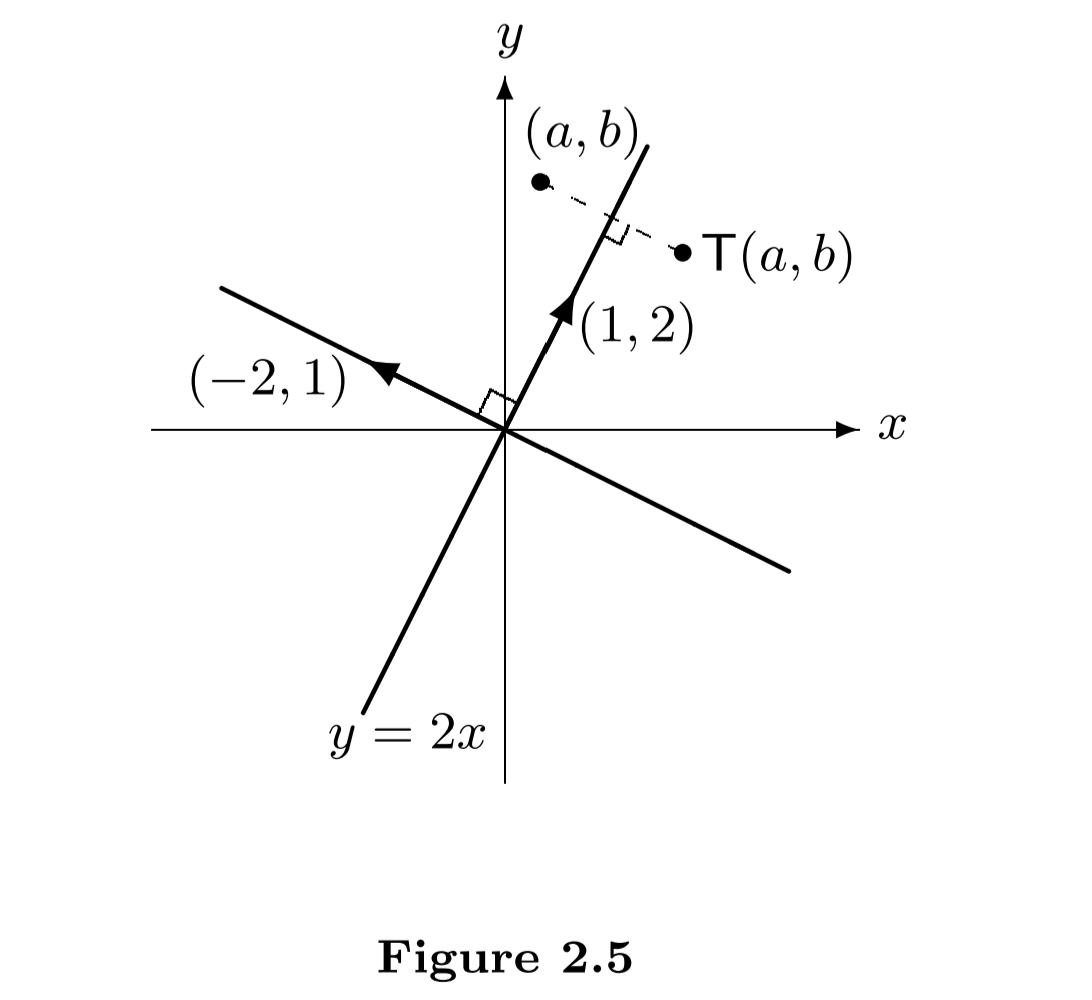
\includegraphics[width=8cm]{images/figure-2-5.png}

\begin{example} \label{example 2.5.3}
Recall the \emph{reflection} about the \(x\)-axis in \EXAMPLE{2.1.3}.
The rule \((x, y) \to (x, -y)\) is easy to obtain.
We now derive the less obvious rule for the \emph{reflection} \(\T\) \emph{about the line} \(y = 2x\). (See Figure 2.5.)

We wish to find \emph{an expression} for \(\T(a,b)\) for any \((a,b) \in \SET{R}^2\).
Since \(\T\) is linear, (by \THM{2.6}) it is completely
determined by its values on \emph{a basis} for \(\SET{R}^2\).
Clearly, from figure 2.5 we have \(\T(1, 2) = (1, 2) = 1 \cdot (1, 2) + 0 \cdot (-2, 1)\) and \(\T(-2, 1) = -(-2, 1) = 0 \cdot (1, 2) + (-1) \cdot (-2, 1)\), where \(\{ (1, 2), (-2, 1) \}\) is a basis for \(\SET{R}^2\).
Then we let \(\beta' = \{ (1, 2), (-2, 1) \}\), from these result (and \THM{2.6}),
\[
    [\T]_{\beta'} = \begin{pmatrix} 1 & 0 \\ 0 & -1 \end{pmatrix}.
\]

Now let \(\beta\) be the \emph{standard} ordered basis for \(\SET{R}^2\), and let \(Q\) be the matrix that changes \(\beta'\)-coordinates into \(\beta\)-coordinates.

Then (by calculation),
\[
    Q = \begin{pmatrix} 1 & -2 \\ 2 & 1 \end{pmatrix}
\]
And from \THM{2.23} and some calculation(see \EXEC{2.5.1}(c)) we have \([\T]_{\beta} = Q[\T]_{\beta'}Q^{-1}\).
Because (mysteriously)
\[
    Q^{-1} = \frac{1}{5} \begin{pmatrix} 1 & 2 \\ -2 & 1 \end{pmatrix}
\]
the reader can verify that
\[
    [\T]_{\beta} = \frac{1}{5} \begin{pmatrix} -3 & 4 \\ 4 & 3 \end{pmatrix}
\]
Since \(\beta\) is the standard ordered basis, it follows by \THM{2.15}(a) that \(\T\) is left-multiplication by \([\T]_{\beta}\).
Thus for any \((a, b) \in \SET{R}^2\), we have
\[
    \T \begin{pmatrix} a \\ b \end{pmatrix}
    = \frac{1}{5} \begin{pmatrix} -3 & 4 \\ 4 & 3 \end{pmatrix} \begin{pmatrix} a \\ b \end{pmatrix}
    = \frac{1}{5} \begin{pmatrix} -3a + 4b \\ 4a + 3b \end{pmatrix}.
\]
\end{example}

A useful special case of \THM{2.23} is contained in the next corollary.

\begin{corollary} \label{corollary 2.23.1}
Let \(A \in M_{n \X n}(F)\), and let \(\gamma\) be an ordered basis for \(F^n\).
Then \([\LMTRAN_A]_{\gamma} = Q^{-1} A Q\), where \(Q\) is the \(n \X n\) matrix whose \(j\)th column is the \(j\)th vector of \(\gamma\).
\end{corollary}

\begin{proof}
Let \(\beta\) be the \emph{standard} ordered basis for \(F^n\), then by \THM{2.15}(a), \([\LMTRAN_A]_{\beta} = A\).
Then by \THM{2.23}, \([\LMTRAN_A]_{\gamma} = Q^{-1} [\LMTRAN_A]_{\beta} Q\) where \(Q\) is the coordinate matrix that changes \(\gamma\)-coordinates into \(\beta\)-coordinates.
And from \RMK{2.5.1}, the \(j\)th column of \(Q\) is \([v_j]_{\beta}\) where \(v_j\) is the \(j\)th vector of \(\gamma\).
But since \(\beta\) is standard ordred basis, we have \([v_j]_{\beta} = v_j\), so the \(j\)th column of \(Q\) is \(v_j\), as desired.
\end{proof}

\begin{note}
這個\ corollary 是\ \RMK{2.5.1} 的「更加\ special case」:
當我們把某個基底座標\textbf{轉換成標準基底座標},則那個座標轉換矩陣的第\ \(j\) 行就直接等於那個基底座標的第\ \(j\) 個向量。
\end{note}

\begin{example} \label{example 2.5.4}
Let
\[
    A = \begin{pmatrix}
        2 & 1 & 0 \\ 1 & 1 & 3 \\ 0 & -1 & 0
    \end{pmatrix},
\]
and let
\[
    \gamma = \bigg\{
        \begin{pmatrix} -1 \\ 0 \\ 0 \end{pmatrix}, 
        \begin{pmatrix} 2 \\ 1 \\ 0 \end{pmatrix}, 
        \begin{pmatrix} 1 \\ 1 \\ 1 \end{pmatrix}
    \bigg\},
\]
which is an ordered basis for \(\SET{R}^3\).
Let \(Q\) be the \(3 \X 3\) matrix whose \(j\)th column is the \(j\)th vector of \(\gamma\). (this satisfies the condition of \CORO{2.23.1}.)
Then
\[
    Q = \begin{pmatrix} -1 & 2 & 1 \\ 0 & 1 & 1 \\ 0 & 0 & 1 \end{pmatrix}
    \text{ and (mysteriously) }
    Q^{-1} = \begin{pmatrix} -1 & 2 & -1 \\ 0 & 1 & -1 \\ 0 & 0 & 1 \end{pmatrix}.
\]
So by \CORO{2.23.1},
\[
    [\LMTRAN_A]_{\gamma} = Q^{-1} A Q = \begin{pmatrix} 0 & 2 & 8 \\ -1 & 4 & 6 \\ 0 & -1 & -1 \end{pmatrix}.
\]
\end{example}

\begin{remark} \label{remark 2.5.2}
The relationship, defined immediately, between the matrices \([\T]_{\beta'}\) and \([\T]_{\beta}\) in \THM{2.23} \textbf{will be the subject of further study in Chapters 5, 6, and 7}.
\end{remark}

\begin{definition} \label{def 2.16}
Let \(A\) and \(B\) be matrices in \(M_{n \X n}(F)\).
We say that \(B\) is \textbf{similar}\textbf{} to \(A\) if there exists an \textbf{invertible matrix} \(Q\) such that \(B = Q^{-1} A Q\).
\end{definition}

\begin{remark} \label{remark 2.5.3}
Observe that the relation of similarity is an \textbf{equivalence relation} (see \EXEC{2.5.9}).
So we need only say that \(A\) and \(B\) are similar.

Notice also that in this terminology \THM{2.23} can be stated as follows:
If \(\T\) is a linear operator on a finite-dimensional vector space \(V\), and if \(\beta\) and \(\beta'\) are any ordered bases for \(V\), then \([\T]_{\beta'}\) is similar to \([\T]_{\beta}\).
\end{remark}

\begin{remark} \label{remark 2.5.4}
\THM{2.23} can be \emph{generalized} to allow \(\T : V \to W\), where \(V\) is distinct from \(W\).
In this case, we can change bases in \(V\) as well as in \(W\) (see \EXEC{2.5.8}).
\end{remark}

\exercisesection

\begin{exercise} \label{exercise 2.5.1}
Label the following statements as true or false.
\begin{enumerate}
\item Suppose that \(\beta = \{ x_1, x_2, ..., x_n \}\) and \(\beta' = \{ x'_1, x'_2, ..., x'_n \}\) are ordered bases for a vector space
and \(Q\) is the change of coordinate matrix that changes \(\beta'\)-coordinates into \(\beta\)-coordinates.
Then the \(j\)th column of \(Q\) is \([x_j]_{\beta'}\).

\item Every change of coordinate matrix is invertible. 

\item Let \(\T\) be a linear operator on a finite-dimensional vector space \(V\), let \(\beta\) and \(\beta'\) be ordered bases for \(V\),
and let \(Q\) be the change of coordinate matrix that changes \(\beta'\)-coordinates into \(\beta\)-coordinates.
Then \([\T]_{\beta} = Q [\T]_{\beta'} Q^{-1}\).

\item The matrices \(A, B \in M_{n \X n}(F)\) are called similar if \(B = Q^\top A Q\) for some \(Q \in M_{n \X n}(F)\).

\item Let \(\T\) be a linear operator on a finite-dimensional vector space \(V\).
Then for any ordered bases \(\beta\) and \(\gamma\) for \(V\), \([\T]_{\beta}\) is similar to \([\T]_{\gamma}\).
\end{enumerate}
\end{exercise}

\begin{proof} \ 

\begin{enumerate}
\item False. By \RMK{2.5.1}, the \(j\)th column of \(Q\) is \([x'_j]_{\beta}\).
\item True by \THM{2.22}(a).
\item True.
    We have
    \begin{align*}
                 & [\T]_{\beta'} = Q^{-1}[\T]_{\beta}Q & \text{by \THM{2.23}} \\
        \implies & Q [\T]_{\beta'} Q^{-1} = Q (Q^{-1} [\T]_{\beta} Q) Q^{-1} & \text{by multiplying \(Q\) in the left and \(Q^{-1}\) in the right} \\
        \implies & Q [\T]_{\beta'} Q^{-1} = [\T]_{\beta},
    \end{align*}
    as desired.
\item False by \DEF{2.16}.
\item True by \RMK{2.5.3}.
\end{enumerate}
\end{proof}

\begin{exercise} \label{exercise 2.5.2}
For each of the following pairs of ordered bases \(\beta\) and \(\beta'\) for \(\SET{R}^2\), find the change of coordinate matrix that changes \(\beta'\)-coordinates into \(\beta\)-coordinates.
\begin{enumerate}
\item \(\beta = \{ e_1, e_2 \}\) and \(\beta' = \{ (a_1, a_2), (b_1, b_2) \}\).
\item \(\beta = \{ (-1, 3), (2, -1) \}\) and \(\beta' = \{ (0, 10), (5, 0) \}\).
\item \(\beta = \{ (2, 5), (-1, -3) \}\) and \(\beta' = \{ e_1, e_2 \}\).
\item \(\beta = \{ (-4, 3), (2, -1) \}\) and \(\beta' = \{ (2, 1), (-4, 1) \}\).
\end{enumerate}
\end{exercise}

\begin{proof} \ 

\begin{enumerate}
\item We have \((a_1, a_2) = a_1 \cdot e_1 + a_2 \cdot e_2\), \((b_1, b_2) = b_1 \cdot e_1 + b_2 \cdot e_2\), so
\[ Q = \begin{pmatrix} a_1 & b_1 \\ a_2 & b_2 \end{pmatrix}. \]

\item (By solving system of equations), \((0, 10) = 4 \cdot (-1, 3) + 2 \cdot (2, -1)\), \((5, 0) = 1 \cdot (-1, 3) + 3 \cdot (2, -1)\), so
\[ Q = \begin{pmatrix} 4 & 1 \\ 2 & 3 \end{pmatrix}. \]

\item (By solving system of equations), \(e_1 = 3 \cdot (2, 5) + 5 \cdot (-1, -3)\), \(e_2 = -1 \cdot (2, 5) + (-2) \cdot (-1, -3)\), so
\[ Q = \begin{pmatrix} 3 & -1 \\ 5 & -2 \end{pmatrix}. \]

\item (By solving system of equations), \((2, 1) = 2 \cdot (-4, 3) + 5 \cdot (2, -1)\), \((-4, 1) = -1 \cdot (-4, 3) + (-4) \cdot (2, -1)\), so
\[ Q = \begin{pmatrix} 2 & -1 \\ 5 & -4 \end{pmatrix}. \]
\end{enumerate}
\end{proof}

\begin{exercise} \label{exercise 2.5.3}
Skip, tedious.
\end{exercise}

\begin{exercise} \label{exercise 2.5.4}
Let \(\T\) be the linear operator on \(\SET{R}^2\) defined by
\[
    \T\begin{pmatrix} a \\ b \end{pmatrix}
    = \begin{pmatrix} 2a + b \\ a - 3b \end{pmatrix},
\]
let \(\beta\) be the standard ordered basis for \(\SET{R}^2\), and let
\[
    \beta' = \bigg\{ \begin{pmatrix} 1 \\ 1 \end{pmatrix},
    \begin{pmatrix} 1 \\ 2 \end{pmatrix} \bigg\}.
\]
Use \THM{2.23} and the (mysterious) fact that
\[
    \begin{pmatrix} 1 & 1 \\ 1 & 2 \end{pmatrix}^{-1} =
    \begin{pmatrix} 2 & -1 \\ -1 & 1 \end{pmatrix}
\]
to find \([\T]_{\beta'}\).
\end{exercise}

\begin{proof}
First \([\T]_{\beta} = \begin{pmatrix} 2 & 1 \\ 1 & -3 \end{pmatrix}\), since \(\T(e_1) = \begin{pmatrix} 2 \\ 1 \end{pmatrix}= 2 \cdot e_1 + 1 \cdot e_2\) and \(\T(e_2) = \begin{pmatrix} 1 \\ -3 \end{pmatrix} = 1 \cdot e_1 + (-3) \cdot e_2\).
And by solving equation we know \(Q = \begin{pmatrix} 1 & 1 \\ 1 & 2 \end{pmatrix}\).
Then by \THM{2.23} and the provided fact,
\[
    [\T]_{\beta'} = Q^{-1} [\T]_{\beta} Q =
    \begin{pmatrix} 2 & -1 \\ -1 & 1 \end{pmatrix}
    \begin{pmatrix} 2 & 1 \\ 1 & -3 \end{pmatrix}
    \begin{pmatrix} 1 & 1 \\ 1 & 2 \end{pmatrix}
    = \begin{pmatrix} 8 & 13 \\ -5 & -9 \end{pmatrix}
\]
\end{proof}

\begin{exercise} \label{exercise 2.5.5}
Let \(\T\) be the linear operator on \(\mathcal{P}_1(\SET{R})\) defined by \(\T(p(x)) = p'(x)\), the derivative of \(p(x)\).\
Let \(\beta = \{ 1, x \}\) and \(\beta' = \{ 1 + x, 1 - x \}\).
Use \THM{2.23} and the fact that
\[
    \begin{pmatrix} 1 & 1 \\ 1 & -1 \end{pmatrix}^{-1} =
    \begin{pmatrix} \frac1{2} & \frac1{2} \\ \frac1{2} & -\frac1{2} \end{pmatrix}
\]
to find \([\T]_{\beta'}\).
\end{exercise}

\begin{proof}

First \([\T]_{\beta} = \begin{pmatrix} 0 & 1 \\ 0 & 0 \end{pmatrix}\) since \(\T(1) = 0 = 0 \cdot 1 + 0 \cdot x\) and \(\T(x) = 1 = 1 \cdot 1 + 0 \cdot x\).
And by solving equation we know \(Q = \begin{pmatrix} 1 & 1 \\ 1 & -1 \end{pmatrix}\).
Then by \THM{2.23} and the provided fact,
\[
    [\T]_{\beta'} = Q^{-1} [\T]_{\beta} Q =
    \begin{pmatrix} \frac1{2} & \frac1{2} \\ \frac1{2} & -\frac1{2} \end{pmatrix}
    \begin{pmatrix} 0 & 1 \\ 0 & 0 \end{pmatrix}
    \begin{pmatrix} 1 & 1 \\ 1 & -1 \end{pmatrix}
    = \begin{pmatrix} \frac1{2} & -\frac1{2} \\ \frac1{2} & -\frac1{2} \end{pmatrix}
\]
\end{proof}

\begin{exercise} \label{exercise 2.5.6}
For each matrix \(A\) and ordered basis \(\beta\), find \([\LMTRAN_A]_{\beta}\).
Also, find an invertible matrix \(Q\) such that \([\LMTRAN_A]_{\beta} = Q^{-1} A Q\).

\begin{enumerate}
\item \(A = \begin{pmatrix} 1 & 3 \\ 1 & 1 \end{pmatrix}\) and \(\beta = \bigg\{
    \begin{pmatrix} 1 \\ 1 \end{pmatrix},
    \begin{pmatrix} 1 \\ 2 \end{pmatrix}
\bigg\}\)

\item \(A = \begin{pmatrix} 1 & 2 \\ 2 & 1 \end{pmatrix}\) and \(\beta = \bigg\{
    \begin{pmatrix} 1 \\ 1 \end{pmatrix},
    \begin{pmatrix} 1 \\ -1 \end{pmatrix}
\bigg\}\)

\item \(A = \begin{pmatrix} 1 & 1 & -1 \\ 2 & 0 & 1 \\ 1 & 1 & 0 \end{pmatrix}\) and \(\beta = \bigg\{
    \begin{pmatrix} 1 \\ 1 \\ 1 \end{pmatrix},
    \begin{pmatrix} 1 \\ 0 \\ 1 \end{pmatrix},
    \begin{pmatrix} 1 \\ 1 \\ 2 \end{pmatrix}
\bigg\}\)

\item \(A = \begin{pmatrix} 13 & 1 & 4 \\ 1 & 13 & 4 \\ 4 & 4 & 10 \end{pmatrix}\) and \(\beta = \bigg\{
    \begin{pmatrix} 1 \\ 1 \\ -2 \end{pmatrix},
    \begin{pmatrix} 1 \\ -1 \\ 0 \end{pmatrix},
    \begin{pmatrix} 1 \\ 1 \\ 1 \end{pmatrix}
\bigg\}\)
\end{enumerate}
\end{exercise}

\begin{proof}
From \CORO{2.23.1}, \([\LMTRAN_A]_{\beta} = Q^{-1} A Q\), where \(Q\) is the \(n \X n\) matrix whose \(j\)th column is the \(j\)th vector of \(\beta\).
Hence

\begin{enumerate}
\item \(Q = \begin{pmatrix} 1 & 1 \\ 1 & 2 \end{pmatrix}\).

\item \(Q = \begin{pmatrix} 1 & 1 \\ 1 & -1 \end{pmatrix}\).

\item \(Q = \begin{pmatrix} 1 & 1 & 1 \\ 1 & 0 & 1 \\ 1 & 1 & 2 \end{pmatrix}\).

\item \(Q = \begin{pmatrix} 1 & 1 & 1 \\ 1 & -1 & 1 \\ -2 & 0 & 1 \end{pmatrix}\).
\end{enumerate}

I skip computing \([\LMTRAN_A]_{\beta}\), since either computing it directly or using \CORO{2.23.1} but requiring \(Q^{-1}\) are tedious.
\end{proof}

\begin{exercise} \label{exercise 2.5.7}
In \(\SET{R}^2\), let \(L\) be the line \(y = mx\), where \(m \ne 0\).
Find an expression for \(\T(x, y)\), where
\begin{enumerate}
\item \(\T\) is the reflection of \(\SET{R}^2\) about \(L\).
\item \(\T\) is the projection(see \ADEF{2.2}) on \(L\) along the line \emph{perpendicular} to \(L\).
\end{enumerate}
\end{exercise}

\begin{proof}
We may let \(\beta\) be the standard ordered basis and \(\alpha = \{ (1, m), (-m, 1) \}\) be another basis for \(\SET{R}^2\).
\begin{enumerate}
\item We have that \([\T]_{\alpha} = \begin{pmatrix} 1 & 0 \\ 0 & -1 \end{pmatrix}\) and (by \EXEC{2.5.11}) \(Q^{-1} = [\mathrm{I}]_{\alpha}^{\beta} = \begin{pmatrix} 1 & m \\ -m & 1 \end{pmatrix}\).
We can also calculate that \(Q = [\mathrm{I}]_{\beta}^{\alpha} = \begin{pmatrix} \frac{1}{m^2 + 1} & \frac{m}{m^2 + 1} \\ -\frac{m}{m^2 + 1} & \frac{1}{m^2 + 1} \end{pmatrix}\).
So by \THM{2.23}, we have
\[
    [\T]_{\beta} = Q^{-1} [\T]_{\alpha} Q = \begin{pmatrix}
        \frac{1 - m^2}{m^2 + 1} & \frac{2m}{m^2 + 1} \\
        \frac{2m}{m^2 + 1} & \frac{m^2 - 1}{m^2 + 1}
    \end{pmatrix}.
\]
And we have
\begin{align*}
    & \T \begin{pmatrix} x \\ y \end{pmatrix} \\
    & = \left[ \T \begin{pmatrix} x \\ y \end{pmatrix} \right]_{\beta} & \text{since domain/codomain are actually \(\SET{R}^n\) and \(\beta\) is standard} \\
    & = [\T]_{\beta} \left[ \begin{pmatrix} x \\ y \end{pmatrix} \right]_{\beta} & \text{by \THM{2.14}} \\
    & = [\T]_{\beta} \begin{pmatrix} x \\ y \end{pmatrix} & \text{since domain/codomain are actually \(\SET{R}^n\) and \(\beta\) is standard} \\
    & = \begin{pmatrix}
            \frac{1 - m^2}{m^2 + 1} & \frac{2m}{m^2 + 1} \\
            \frac{2m}{m^2 + 1} & \frac{m^2 - 1}{m^2 + 1}
        \end{pmatrix}
        \begin{pmatrix} x \\ y \end{pmatrix} \\
    & = \begin{pmatrix}
            \frac{x-m^{2} x+2 m y}{1+m^{2}} \\
            \frac{2 m x+m^{2} y-y}{1+m^{2}}
        \end{pmatrix}
\end{align*}

\item Similarly we have that \([\T]_{\alpha} = \begin{pmatrix} 1 & 0 \\ 0 & 0 \end{pmatrix}\).
And with the same \(Q^{-1}\) and \(Q\) we have
\[
    [\T]_{\beta} = Q^{-1} [\T]_{\alpha} Q = \begin{pmatrix}
        \frac{1}{m^2 + 1} & \frac{m}{m^2 + 1} \\
        \frac{m}{m^2 + 1} & \frac{m^2}{m^2 + 1}
    \end{pmatrix}.
\]
So 
\begin{align*}
    & \T \begin{pmatrix} x \\ y \end{pmatrix} \\
    & = [\T]_{\beta} \begin{pmatrix} x \\ y \end{pmatrix} & \text{similar derivation from part(a)} \\
    & = \begin{pmatrix}
            \frac{1}{m^2 + 1} & \frac{m}{m^2 + 1} \\
            \frac{m}{m^2 + 1} & \frac{m^2}{m^2 + 1}
        \end{pmatrix}
        \begin{pmatrix} x \\ y \end{pmatrix} \\
    & = \begin{pmatrix}
            \frac{x + ym}{m^{2} + 1} \\
            \frac{xm + ym^2}{m^{2} + 1}
        \end{pmatrix}
\end{align*}

\end{enumerate}
\end{proof}

\begin{exercise} \label{exercise 2.5.8}
Prove the following \emph{generalization} of \THM{2.23}.
Let \(\T : V \to W\) be a \LTRAN{} from a finite-dimensional vector space \(V\) to a finite-dimensional vector space \(W\).
Let \(\beta\) and \(\beta'\) be ordered bases for \(V\), and let \(\gamma\) and \(\gamma'\) be ordered bases for \(W\).
Then \([\T]_{\beta'}^{\gamma'} = P^{-1} [\T]_{\beta}^{\gamma} Q\), where \(Q\) is the matrix that changes \(\beta'\)-coordinates into \(\beta\)-coordinates and \(P\) is the matrix that changes \(\gamma'\)-coordinates into \(\gamma\)-coordinates.
\end{exercise}

\begin{proof}
By (the generalization of) \THM{2.10}(c), we have \(\T = \ITRANW \T = \T \ITRANV\) \MAROON{(1)}.

Then we have
\begin{align*}
    P [\T]_{\beta'}^{\gamma'}
        & = [\ITRANW]_{\gamma'}^{\gamma} [\T]_{\beta'}^{\gamma'} & \text{by def of \(P\)} \\
        & = [\ITRANW\T]_{\beta'}^{\gamma} & \text{by \THM{2.11}} \\
        & = [\T\ITRANV]_{\beta'}^{\gamma} & \text{by \MAROON{(1)}} \\
        & = [\T]_{\beta}^{\gamma} [\ITRANV]_{\beta'}^{\beta} & \text{\THM{2.11}} \\
        & = [\T]_{\beta}^{\gamma} Q & \text{by def of \(Q\)}
\end{align*}
So we have \(P [\T]_{\beta'}^{\gamma'} = [\T]_{\beta}^{\gamma} Q\).
And
\begin{align*}
             & P [\T]_{\beta'}^{\gamma'} = [\T]_{\beta}^{\gamma} Q \\
    \implies & P^{-1} P [\T]_{\beta'}^{\gamma'} = P^{-1} [\T]_{\beta}^{\gamma} Q & \text{by multiplying \(P^{-1}\) in the left} \\
    \implies & [\T]_{\beta'}^{\gamma'} = P^{-1} [\T]_{\beta}^{\gamma} Q, & \text{of course}
\end{align*}
as desired.
\end{proof}

\begin{exercise} \label{exercise 2.5.9}
Prove that "is similar to" is an equivalence relation on \(M_{n \X n}(F)\).
\end{exercise}

\begin{proof}
For any \(n \X n\) matrix \(A\), it is similar to itself since \(A = IAI\).

Suppose \(A\) is similar to \(B\), then by \DEF{2.16} we have an invertible matrix \(Q\) s.t. \(A = Q^{-1}BQ\).
Then
\begin{align*}
             & A = Q^{-1}BQ \\
    \implies & Q A Q^{-1} = Q (Q^{-1} B Q) Q^{-1} \\
    \implies & Q A Q^{-1} = B \\
    \implies & (Q^{-1})^{-1} A Q^{-1} = B.
\end{align*}
So we have an invertible matrix \(Q^{-1}\) s.t. \(B = (Q^{-1})^{-1} A Q^{-1}\).
Then by \DEF{2.16}, \(B\) is similar to \(A\).

Suppose \(A\) is similar to \(B\), \(B\) is similar to \(C\).
Then by \DEF{2.16} we have an invertible matrix \(P\) s.t. \(A = P^{-1}BP\) and invertible matrix \(Q\) s.t. \(B = Q^{-1}CQ\)
Then by \ATHM{2.36}(2), \(QP\) is invertible and \((QP)^{-1} = P^{-1} Q^{-1}\) \MAROON{(1)}.
And
\begin{align*}
             & A = P^{-1}BP \\
    \implies & A = P^{-1} (Q^{-1} C Q) P \\
    \implies & A = (P^{-1} Q^{-1}) C (Q P) \\
    \implies & A = (Q P)^{-1} C (Q P) & \text{by \MAROON{(1)}}
\end{align*}
So we have an invertible matrix \(QP\) s.t. \(A = (QP)^{-1} C (QP)\).
So by \DEF{2.16}, \(A\) is similar to \(C\).
\end{proof}

\begin{exercise} \label{exercise 2.5.10} \ 

\begin{enumerate}
\item Prove that if \(A\) and \(B\) are similar \(n \X n\) matrices, then \(\TRACE(A) = \TRACE(B)\).
Hint: Use \ATHM{2.27}.
USEDINSEC5.2\#11.

\item How would you define the \emph{trace} of a linear operator on a finite-dimensional vector space?
Justify that your definition is well-defined.
\end{enumerate}
\end{exercise}

\begin{proof} \ 

\begin{enumerate}
\item
\begin{align*}
    \TRACE(A) & = \TRACE(\BLUE{Q^{-1}B}\RED{Q}) & \text{since \(A, B\) are similar} \\
              & = \TRACE(\RED{Q}\BLUE{Q^{-1}B}) & \text{by \ATHM{2.27}} \\
              & = \TRACE(B) & \text{of course}
\end{align*}

\item Given finite-dimensional vector space \(V\) and linear operator \(\T : V \to V\), we define \(\TRACE(\T) = \TRACE([\T]_{\beta})\) where \(\beta\) is a basis for \(V\).
The definition is well-defined because given arbitrary bases \(\beta, \beta'\) for \(V\), by \THM{2.23}, \([\T]_{\beta}\) and \([\T]_{\beta'}\) are similar, and by part(a), \(\TRACE([\T]_{\beta}) = \TRACE([\T]_{\beta'})\).
\end{enumerate}
\end{proof}

\begin{exercise} \label{exercise 2.5.11}
Let \(V\) be a finite-dimensional vector space with ordered bases \(\alpha, \beta\), and \(\gamma\).
\begin{enumerate}
\item Prove that if \(Q\) and \(R\) are the change of coordinate matrices that change \(\alpha\)-coordinates into \(\beta\)-coordinates and \(\beta\)-coordinates into \(\gamma\)-coordinates, respectively, then \(RQ\) is the change of coordinate matrix that changes \(\alpha\)-coordinates into \(\gamma\)-coordinates.

\item Prove that if \(Q\) changes \(\alpha\)-coordinates into \(\beta\)-coordinates, then \(Q^{-1}\) changes \(\beta\)-coordinates into \(\alpha\)-coordinates.
\end{enumerate}
\end{exercise}

\begin{proof} \ 
\begin{enumerate}
\item We have \(Q = [\mathrm{I}]_{\alpha}^{\beta}\) and \(R = [\mathrm{I}]_{\beta}^{\gamma}\).
So
\begin{align*}
    RQ = & [\mathrm{I}]_{\beta}^{\gamma} [\mathrm{I}]_{\alpha}^{\beta} \\
         & = [\mathrm{I}\mathrm{I}]_{\alpha}^{\gamma} & \text{by \THM{2.11}} \\
         & = [\mathrm{I}]_{\alpha}^{\gamma}, & \text{of course}
\end{align*}
which is the coordinate matrix that change \(\alpha\)-coordinates into \(\gamma\)-coordinates.

\item Again we have \(Q = [\mathrm{I}]_{\alpha}^{\beta}\).
Let \(I_n\) be \(n \X n\) identity matrix, then we have
\begin{align*}
    Q[\mathrm{I}]_{\beta}^{\alpha}
        & = [\mathrm{I}]_{\alpha}^{\beta}[\mathrm{I}]_{\beta}^{\alpha} \\
        & = [\mathrm{I}\mathrm{I}]_{\beta}^{\beta} & \text{by \THM{2.11}} \\
        & = [\mathrm{I}]_{\beta}^{\beta} & \text{of course} \\
        & = I_n, & \text{of course}
\end{align*}
and
\begin{align*}
    [\mathrm{I}]_{\beta}^{\alpha} Q
        & = [\mathrm{I}]_{\beta}^{\alpha} [\mathrm{I}]_{\alpha}^{\beta} \\
        & = [\mathrm{I}\mathrm{I}]_{\alpha}^{\alpha} & \text{by \THM{2.11}} \\
        & = [\mathrm{I}]_{\alpha}^{\alpha} & \text{of course} \\
        & = I_n, & \text{of course}
\end{align*}
hence by definition of \DEF{2.13}, \(Q^{-1}\) is \([\mathrm{I}]_{\beta}^{\alpha}\), that is, \(Q^{-1}\) is the coordinate matrix that changes \(\beta\)-coordinates into \(\alpha\)-coordinates.
\end{enumerate}
\end{proof}

\begin{exercise} \label{exercise 2.5.12}
Prove \CORO{2.23.1}.
\end{exercise}

\begin{proof}
See \CORO{2.23.1}.
\end{proof}

\begin{exercise} \label{exercise 2.5.13}
\sloppy Let \(V\) be a finite-dimensional vector space over a field \(F\), and let \(\beta = \{ x_1, x_2, ..., x_n \}\) be an ordered basis for \(V\).
Let \(Q\) be an \(n \X n\) \emph{invertible} matrix with entries from \(F\).
Define
\[
    x_j' = \sum_{i = 1}^n Q_{ij} x_i \text{ for } 1 \le j \le n,
\]
and set \(\beta' = \{ x_1', x_2', ..., x_n' \}\).
Prove that \(\beta'\) is a basis for \(V\) and hence that \(Q\) is the change of coordinate matrix that changes \(\beta'\)-coordinates into \(\beta\)-coordinates.
\end{exercise}

\begin{note}
The exercise with highly related concept: \EXEC{2.4.15}.
\end{note}

\begin{note}
這題背後的意義就是,若\ \(\beta\) 是\ basis,\(\T\) 是可逆變換(所以對應的矩陣也是可逆),則\ \(\T(\beta)\) 也是一個\ basis。
相關練習有\ \EXEC{2.4.15},不過這題是那個練習的\ special case,也就是\ codomain \(W = V\) 的情況。
\end{note}

\begin{proof}
First we show that \(\beta'\) is \LID{}.
So suppose \(a_1 x'_1 + a_2 x'_2 + ... + a_n x'_n = \OV\), we have to show \(a_1 = a_2 = ... = a_n = 0\).
Then
\begin{align*}
             & \sum_{j = 1}^n a_j x'_j = \OV \\
    \implies & \sum_{j = 1}^n a_j \bigg( \sum_{i = 1}^n Q_{ij} x_i \bigg) = \OV & \text{by def of \(x'_j\)} \\
    \implies & \sum_{j = 1}^n \bigg( \sum_{i = 1}^n Q_{ij} a_j x_i \bigg) = \OV & \text{move constant into summation} \\
    \implies & \sum_{i = 1}^n \bigg( \sum_{j = 1}^n Q_{ij} a_j x_i \bigg) = \OV, & \text{change the order of finite summation} \\
    \implies & \sum_{i = 1}^n \bigg( \sum_{j = 1}^n Q_{ij} a_j \bigg) x_i = \OV & \text{of course}
\end{align*}
which implies \(\sum_{j = 1}^n Q_{ij} a_j = 0\) for all \(1 \le i \le n\) since \(x_i\) are \LID{}.
But that implies
\begin{align*}
    \begin{pmatrix} 0 \\ 0 \\ \vdots \\ 0 \end{pmatrix}
    & = \begin{pmatrix}
        \sum_{j = 1}^n Q_{1j} a_j \\
        \sum_{j = 1}^n Q_{2j} a_j \\
        \vdots \\
        \sum_{j = 1}^n Q_{nj} a_j
    \end{pmatrix} \\
    & = Q \begin{pmatrix} a_1 \\ a_2 \\ \vdots \\ a_n \end{pmatrix} & \text{it's true but it's more intuitive from RHS to LHS}
\end{align*}
And since \(Q\) is invertible, we have
\begin{align*}
             & \begin{pmatrix} 0 \\ 0 \\ \vdots \\ 0 \end{pmatrix}
    = Q \begin{pmatrix} a_1 \\ a_2 \\ \vdots \\ a_n \end{pmatrix} \\
    \implies & \begin{pmatrix} 0 \\ 0 \\ \vdots \\ 0 \end{pmatrix} = Q^{-1} \begin{pmatrix} 0 \\ 0 \\ \vdots \\ 0 \end{pmatrix}
    = Q^{-1} Q \begin{pmatrix} a_1 \\ a_2 \\ \vdots \\ a_n \end{pmatrix} \\
    \implies & \begin{pmatrix} 0 \\ 0 \\ \vdots \\ 0 \end{pmatrix}
    = \begin{pmatrix} a_1 \\ a_2 \\ \vdots \\ a_n \end{pmatrix} \\
    \implies & a_1 = a_2 = ... = a_n = 0
\end{align*}
Hence \(\beta' = \{ x'_1, x'_2, ..., x'_n \}\) is \LID{}.
Since \(\beta'\) has \(n\) vectors, it is a basis for \(V\).

Now from the definition of \(x'_j\), we know \([x'_j]_{\beta}\) is equal to the \(j\)th column of \(Q\), but \([x'_j]_{\beta}\), which is equal to \([\mathrm{I}(x'_j)]_{\beta}\),
is (by definition of matrix representation) also equal to the \(j\)th column of \([\mathrm{I}]_{\beta'}^{\beta}\), hence \(Q = [\mathrm{I}]_{\beta'}^{\beta}\).
That is, \(Q\) is the coordinate matrix that changes \(\beta'\)-coordinates into \(\beta\)-coordinates.
\end{proof}

\begin{exercise} \label{exercise 2.5.14}
Prove the \emph{converse} of \EXEC{2.5.8}:
If \(A\) and \(B\) are each \(m \X n\) matrices with entries from a field \(F\), and if there exist \emph{invertible} \(m \X m\) and \(n \X n\) matrices \(P\) and \(Q\), respectively,
such that \(B = P^{-1} A Q\) \MAROON{(1)}, then there exist an \(n\)-dimensional vector space \(V\) and an \(m\)-dimensional vector space \(W\) (both over \(F\)), ordered bases \(\beta\) and \(\beta'\) for \(V\) and \(\gamma\) and \(\gamma'\) for \(W\),
and a \LTRAN{} \(\T : V \to W\) such that
\[
    A = [\T]_{\beta}^{\gamma} \text{ and } B = [\T]_{\beta'}^{\gamma'}.
\]
Hints: Let \(V = F^n\), \(W = F^m\), \(\T = \LMTRAN_A\), and \(\beta\) and \(\gamma\) be the \emph{standard} ordered bases for \(F^n\) and \(F^m\), respectively.
Now apply the results of \EXEC{2.5.13} to obtain ordered bases \(\beta'\) and \(\gamma'\) from \(\beta\) and \(\gamma\) via \(Q\) and \(P\), respectively.
\end{exercise}

\begin{proof}
Let \(V = F^n\), \(W = F^m\), \(\T = \LMTRAN_A\), \(\beta = \{ e_1, e_2, ..., e_n \}\) be the standard ordered basis for \(F^n\), \(\gamma = \{ f_1, f_2, ..., f_m \}\) be the standard ordered basis for \(F^m\).

Then let \(\beta' = \{ v_1, v_2, ..., v_n \}\), where \(v_j = \sum_{i = 1}^n Q_{ij} e_i\) and \(\gamma' = \{ w_1, w_2, ..., w_m \}\), where \(w_j = \sum_{i = 1}^m P_{ij} f_i\).
Then by \EXEC{2.5.13}, \(\beta', \gamma'\) are also bases for \(V\) and \(W\), respectively;
furthermore, \(Q\) is the coordinate matrix that changes \(\beta'\)-coordinates into \(\beta\) coordinates,
and \(P\) is the coordinate matrix that changes \(\gamma'\)-coordinates into \(\gamma\) coordinates.

Then since \(\beta, \gamma\) are standard bases, by \THM{2.15}(a) we have \([\T]_{\beta}^{\gamma} = [\LMTRAN_A]_{\beta}^{\gamma} = A\) \MAROON{(2)}.

And
\begin{align*}
    [\T]_{\beta'}^{\gamma'}
        & = [\LMTRAN_A]_{\beta'}^{\gamma'} \\
        & = P^{-1} [\LMTRAN_A]_{\beta}^{\gamma} Q & \text{by \EXEC{2.5.8}} \\
        & = P^{-1} A Q & \text{by \MAROON{(2)}} \\
        & = B & \text{by \MAROON{(1)}}
\end{align*}

So we have found \(V, W\), a \LTRAN{} \(\T : V \to W\), and bases \(\beta, \beta', \gamma, \gamma'\), s.t. \(A = [\T]_{\beta}^{\gamma} \text{ and } B = [\T]_{\beta'}^{\gamma'}\), as desired.
\end{proof}

\begin{additional theorem} \label{athm 2.46} \ 

\BLUE{(1)} This is the placeholder theorem for \EXEC{2.5.8}, the generalization of \THM{2.23}.

\BLUE{(2)} This is the placeholder theorem for \EXEC{2.5.14}, which is the \emph{converse} of \EXEC{2.5.8}.
\end{additional theorem}

\begin{additional theorem} \label{athm 2.47}
This is the placeholder theorem for \EXEC{2.5.9}: similarity is an equivalence relation.
\end{additional theorem}

\begin{additional theorem} \label{athm 2.48}
This is the placeholder theorem for \EXEC{2.5.10}:

\BLUE{(1)}: If \(A, B\) are similar \(n \X n\) matrices, then \(\TRACE(A) = \TRACE(B)\).

\BLUE{(2)}: Given finite-dimensional vector space \(V\) and linear operator \(\T : V \to V\), we can define \(\TRACE(\T) = \TRACE([\T]_{\beta})\) where \(\beta\) is a basis for \(V\), and the definition is well-defined.
\end{additional theorem}

\begin{additional theorem} \label{athm 2.49}
This is the placeholder theorem for \EXEC{2.5.11}:

\BLUE{(1)} If \(Q = [\mathrm{I}]_{\alpha}^{\beta}\) and \(R = [\mathrm{I}]_{\beta}^{\gamma}\), then \(RQ = [\mathrm{I}]_{\alpha}^{\gamma}\).

\BLUE{(2)} If \(Q = [\mathrm{I}]_{\alpha}^{\beta}\), then \(Q^{-1} = [\mathrm{I}]_{\beta}^{\alpha}\).
\end{additional theorem}

\begin{additional theorem} \label{athm 2.50}
This is the placeholder theorem for \EXEC{2.5.13}:

\sloppy Let \(V\) be a finite-dimensional vector space over a field \(F\), and let \(\beta = \{ x_1, x_2, ..., x_n \}\) be an ordered basis for \(V\).
Let \(Q\) be an \(n \X n\) \emph{invertible} matrix with entries from \(F\).
Define
\[
    x_j' = \sum_{i = 1}^n Q_{ij} x_i \text{ for } 1 \le j \le n,
\]
and set \(\beta' = \{ x_1', x_2', ..., x_n' \}\).
Then \(\beta'\) is a basis for \(V\) and hence that \(Q\) is the change of coordinate matrix that changes \(\beta'\)-coordinates into \(\beta\)-coordinates.
\end{additional theorem}
